%% Supplementary Material -- compiled separately from main.tex
%% Phase 8 (drafting order step 12): supplement S1..S9, written from the
%% frozen claim set (papers/governance/claims_evidence_matrix.csv), the Phase 7
%% caption registry (papers/build_prompt_phases/phase_07/captions_registry.md),
%% and papers/governance/artifact_binding.csv. Every empirical value traces to
%% evidence release rel-2026-07-20-67d9345f9 (supersedes rel-2026-07-16-78f075cb0).
\documentclass[algorithms,article,submit,moreauthors,pdftex]{Definitions/mdpi}

%=================================================================
\firstpage{1}
\makeatletter
\setcounter{page}{\@firstpage}
\makeatother
\pubvolume{xx}
\issuenum{1}
\articlenumber{5}
\pubyear{2026}
\copyrightyear{2026}
\history{Received: date; Accepted: date; Published: date}

%------------------------------------------------------------------
% Additional packages
%------------------------------------------------------------------
% Suppress MDPI class "submit" mode line numbers without having to
% switch to "accept" (which requires a journal-specific logo file we
% do not ship).  The class issues \linenumbers in submit mode; turning
% it into a no-op cleanly disables left-margin line numbering.
% SE-048: submit-mode line numbering RESTORED 2026-07-22 -- MDPI review
% copies carry left-margin line numbers so reviewers can anchor comments.
% Verified not to disturb validate_cross_format_parity (squash-containment).
% SE-048 REVERSED 2026-07-24 (author decision): line numbering DISABLED again.
% Re-enable by re-commenting the line below; parity is unaffected either way.
\let\linenumbers\relax
\usepackage{amssymb}
\usepackage[ruled,vlined,linesnumbered]{algorithm2e}
\SetAlgoSkip{smallskip}
\SetAlgoInsideSkip{smallskip}
\SetKwComment{tcp}{\textit{// }}{}
\SetKwComment{tcc}{\textit{/* }}{\textit{ */}}
\usepackage{bm}
\usepackage{longtable}
\usepackage{siunitx}
\usepackage{subcaption}
\usepackage{pgfplots}
\pgfplotsset{compat=1.18}
\usetikzlibrary{shapes.geometric, arrows.meta, positioning, calc}
\usepackage{rotating}
\usepackage{pdflscape} % CR-007: true landscape pages (sets /Rotate) for wide tables

%------------------------------------------------------------------
% Custom macros (identical to main.tex)
%------------------------------------------------------------------
\newcommand{\dtgsk}{DT-GSK}
\newcommand{\sgsm}{ISM}
\newcommand{\atmals}{ATMALS-GSK}
\newcommand{\agsk}{AGSK}
\newcommand{\apgsk}{APGSK}
\newcommand{\fdbagsk}{FDB-AGSK}
\newcommand{\egsk}{eGSK}
\newcommand{\bestval}[1]{\textbf{#1}}
\newcommand{\wmark}{\ensuremath{+}}
\newcommand{\lmark}{\ensuremath{-}}
\newcommand{\emark}{\ensuremath{\approx}}
\DeclareMathOperator*{\argmin}{arg\,min}
\DeclareMathOperator*{\argmax}{arg\,max}

% Zebra striping for data tables (matches main.tex; the generated table
% fragments begin with \zebra). xcolor[table] is provided by the MDPI class.
\definecolor{zebragray}{gray}{0.94}
\newcommand{\zebra}{\rowcolors{2}{zebragray}{white}}

% SI column type for tables
\sisetup{
  table-format=1.2e+2,
  round-mode=places,
  round-precision=2,
  scientific-notation=true,
  exponent-product=\times,
}

%=================================================================
% Title
% Gate 8 QA fix (2026-07-11): title aligned to the main document's frozen
% Phase-8 title (main.tex \Title) -- stale "Adaptive" removed.
\Title{Supplementary Material for: DT-GSK: Dimension-Tiered Adaptive Configuration Selection and Deterministic Refinement for Gaining-Sharing Knowledge Optimization}

% Author ORCID IDs. Kept in sync with main.tex:113-115; the iDs are written
% literally in the \address block below because pandoc does not expand custom
% macros (see main.tex for the same note). Placeholder zeros were replaced with
% the real iDs on 2026-08-01 (audit finding HYG-14); the macros remain unused,
% so the rendered output is unchanged.
\newcommand{\orcidauthorA}{0009-0003-8415-2158}
\newcommand{\orcidauthorB}{0000-0003-0387-5876}
\newcommand{\orcidauthorC}{0000-0002-5895-2632}

% Authors
\Author{Mostafa Elsayed Masoud $^{1,}$*, Heba Sayed Mohamed Roshdy $^{1}$ and Ali Wagdy Mohamed $^{1}$}

% Authors for PDF metadata
\AuthorNames{Mostafa Elsayed Masoud, Heba Sayed Mohamed Roshdy, Ali Wagdy Mohamed}

% Affiliations
% AG-0005 CLOSED 2026-07-25: H.S.M.R. e-mail supplied by the author. Her address
% was previously OMITTED here (the main paper carried a bracketed placeholder
% instead), so the two documents listed different contact sets -- now aligned.
% ORCID iD written literally, not via \orcidauthorB: pandoc does not expand custom
% macros, so the macro form would vanish from the DOCX (see main.tex).
\address{%
$^{1}$ \quad Operations Research Department, Faculty of Graduate Studies for
Statistical Research, Cairo University, Giza 12613, Egypt;
moustafa.masoud@gmail.com (M.E.M.\ ORCID 0009-0003-8415-2158); hmhmdss@yahoo.com (H.S.M.R.\ ORCID 0000-0003-0387-5876); aliwagdy@gmail.com (A.W.M.\ ORCID 0000-0002-5895-2632)}
% Affiliations 2 (Applied Science Private University, Amman) and 3 (Chitkara
% University, Rajpura) removed at the author's direction on 2026-07-29,
% matching main.tex; all three authors carry affiliation 1 only.

% Corresponding author
\corres{Correspondence: moustafa.masoud@gmail.com}

%=================================================================
% Abstract (supplement scope statement only; no result values)
\abstract{%
This Supplementary Material accompanies the main paper on
Dimension-Tiered Gaining-Sharing Knowledge (\dtgsk{})
optimization.  It contains the complete per-function CEC2017 panel
tables (Section~S1), the \dtgsk{}-versus-GSK head-to-head matrices and the
CEC2011 and CEC2013 detail tables (Section~S2), the convergence
figure sets for CEC2017, CEC2011 and CEC2013 (every scored function at the
prespecified dimensions, Section~S3), a population-reduction schedule
and diagnostic-availability note (Section~S4), a reproducibility appendix documenting
the seed schedule, the frozen configuration, the evidence release, and
the analysis pipeline (Section~S5), a supplement-only
component-contribution study (a scaffold remove-one ablation, a
direct interaction-structure-memory isolation, and a by-class conditional-benefit
breakdown, Section~S6), the complete CEC2013LSGO large-scale suite record
(protocol, evidential tiers, family statistics, effect sizes, and
per-function detail, Section~S7), and the pre-registered CEC2020
confirmatory suite record (Section~S8), and the mechanism-isolation and
sensitivity experiments (Section~S9).  Every empirical value in Sections~S1--S5 derives from the
promoted, read-only evidence release accompanying this article;
the Section~S6 scaffold and isolation results derive from a separate, immutable
ablation release; the Section~S7, Section~S8 and Section~S9 values derive from
further separate, non-superseding evidence releases named where they are used;
no primary result is
altered by any of it.  All comparative
wording is scoped to the seven-algorithm GSK-family panel.%
}

% Keywords
\keyword{%
metaheuristic optimization;
gaining-sharing knowledge;
dimension-tiered adaptive configuration selection;
deterministic final refinement;
adaptive operator selection;
population-size reduction;
CEC benchmark suites;
nonparametric statistical comparison;
reproducibility%
}

%%%%%%%%%%%%%%%%%%%%%%%%%%%%%%%%%%%%%%%%%%
\begin{document}

% Supplement numbering scheme (presentation register, Dimension 20):
% sections S1..S9; tables A.n; figures B.n; every exhibit cited by exact label.
\renewcommand{\thesection}{S\arabic{section}}
\renewcommand{\thesubsection}{S\arabic{section}.\arabic{subsection}}
\renewcommand{\thetable}{A\arabic{table}}
\renewcommand{\thefigure}{B\arabic{figure}}
\setcounter{section}{0}

%==================================================================
% Shared protocol facts (stated once; repeated inside captions so that
% every caption is self-contained, per the caption registry conventions).
%==================================================================
\noindent This Supplementary Material is organized so that the main paper
remains auditable without it: the headline comparative claims are supported
by main-text exhibits, and the material here provides the complete
per-function, per-problem, and per-checkpoint record behind those
exhibits.  Unless a caption states otherwise, the following frozen
protocol applies throughout.
CEC2017 is the primary suite with 29 scored functions (F1, F3--F30; F2 is
excluded per protocol), $D \in \{10, 30, 50, 100\}$, 51 runs per
(function, dimension) cell, and $\mathrm{MaxFES} = 10^{4} \cdot D$~\cite{awad2016problem}.
% BIND: PR-01; PR-04
CEC2011 comprises 22 real-world problems at their native dimensions with
25 runs per problem and $\mathrm{MaxFES} = 150{,}000$; on problems without
published optima the error column is undefined by design and the raw best
objective value is authoritative~\cite{das2011cec2011}.
% BIND: PR-02; PR-04
CEC2013 is the second comparison suite, reported for breadth of
comparison: 28 functions, $D \in \{10, 30, 50\}$, 51 runs per
cell, and $\mathrm{MaxFES} = 10^{4}\,D$~\cite{liang2013cec2013}.
% BIND: PR-03; AN-PW-2013-D10..D50 (n=28, 51 runs; seed_and_pairing_audit.md: 4,284 = 3 x 28 x 51 schedule rows)
CEC2020 is the pre-registered confirmatory suite: 10 functions at
$D \in \{5, 10, 15, 20\}$, with F6 and F7 undefined at $D = 5$ (38 scored
cells), 30 runs per cell, and a dimension-dependent budget of
$\mathrm{MaxFES} = 5 \times 10^{4}$, $10^{6}$, $3 \times 10^{6}$ and
$10^{7}$ at $D = 5, 10, 15, 20$ respectively~\cite{yue2020cec2020}.
% BIND: RS-12; addendum Section 2 (Section~S8)
CEC2013LSGO is the large-scale suite, family-internal by registered scope:
15 functions at native $D = 1000$ (F13/F14 at $D = 905$), 25 runs per
function, $\mathrm{MaxFES} = 3 \times 10^{6}$, reported on the raw
best-objective basis~\cite{li2013lsgo}.
% BIND: RS-13; addendum Section 2 (Section~S7)
CEC2017, CEC2013 and CEC2020 report the final error $f(x) - f(x^{*})$ with
the suite success floor (error values below $10^{-8}$ are treated as zero
per suite convention); CEC2011 and CEC2013LSGO are raw-objective suites.
% BIND: PR-05; addendum Section 2
The run counts (51/25/51/30/25 for CEC2017/CEC2011/CEC2013/CEC2020/%
CEC2013LSGO) and endpoint bases (error vs.\ raw objective) are
heterogeneous across suites by each suite's own convention, and no
statistic in this paper ever pools suites: there is no cross-suite
Friedman family, no pooled run set, no cross-suite rank averaging, and no
cross-suite multiplicity family; the only cross-suite statement made
anywhere is the count of independent per-suite descriptive standings.
% BIND: addendum Section 8 (absolute pooling prohibition)
Pairwise inference uses the two-sided Wilcoxon signed-rank
test~\cite{wilcoxon1945individual} with Holm's step-down
correction~\cite{holm1979simple} at family level and $\alpha = 0.05$;
win/tie/loss counts use the tie rule $|\Delta| < 10^{-8}$.
% BIND: AN-PW-2017-D10..D100 protocol constants (captions_registry.md conventions block)
Panel ranking uses the Friedman test~\cite{friedman1937use} with the
Iman--Davenport correction and Nemenyi post-hoc critical-difference (CD)
analysis~\cite{demsar2006statistical}.
% BIND: AN-OMNI-2017-D10..D100
The panel order everywhere is GSK, \agsk{}, \apgsk{}, \fdbagsk{},
\atmals{}, \egsk{}, \dtgsk{}, and all comparative wording is scoped
within the GSK-family panel, never field-wide.

%==================================================================
\section{Complete CEC2017 Per-Function Panel Tables}\label{sec:supp:cec2017-tables}
%==================================================================

Table~\ref{tab:cec2017-functions} lists the 29 scored CEC2017 functions with
their class in the suite taxonomy and their known optimal value, so the
function-class reading in Section~\ref{sec:supp:ablation:subset} can be checked
against a stated inventory rather than an implicit one.

\begin{table}[H]
\caption{CEC2017 scored-function inventory: class and known optimal value
$f^{*}$ for each of the 29 scored functions. The class boundaries and the
$f^{*}(F_{i}) = 100i$ rule are read from the benchmark suite definition
(benchmarks/cec\_suite\_python/cec2017/functions.py), not from a
secondary source. F2 is excluded under the adopted protocol because of
documented instability, uniformly in every panel cell, and so does not
appear.}\label{tab:cec2017-functions}
% BIND: generated by papers/scripts/generate_function_inventory.py from the
% suite definition -- read, never hand-transcribed
\centering
\tablesize{\footnotesize}
\zebra
\begin{tabular}{llr}
\toprule
\textbf{Function} & \textbf{Class} & \textbf{$f^{*}$} \\
\midrule
F1 & Unimodal & 100 \\
F3 & Unimodal & 300 \\
F4 & Simple multimodal & 400 \\
F5 & Simple multimodal & 500 \\
F6 & Simple multimodal & 600 \\
F7 & Simple multimodal & 700 \\
F8 & Simple multimodal & 800 \\
F9 & Simple multimodal & 900 \\
F10 & Simple multimodal & 1000 \\
F11 & Hybrid & 1100 \\
F12 & Hybrid & 1200 \\
F13 & Hybrid & 1300 \\
F14 & Hybrid & 1400 \\
F15 & Hybrid & 1500 \\
F16 & Hybrid & 1600 \\
F17 & Hybrid & 1700 \\
F18 & Hybrid & 1800 \\
F19 & Hybrid & 1900 \\
F20 & Hybrid & 2000 \\
F21 & Composition & 2100 \\
F22 & Composition & 2200 \\
F23 & Composition & 2300 \\
F24 & Composition & 2400 \\
F25 & Composition & 2500 \\
F26 & Composition & 2600 \\
F27 & Composition & 2700 \\
F28 & Composition & 2800 \\
F29 & Composition & 2900 \\
F30 & Composition & 3000 \\
\bottomrule
\end{tabular}

\end{table}

Tables~\ref{tab:cec2017-d10}--\ref{tab:cec2017-d100} give the complete
seven-algorithm per-function record on CEC2017: mean $\pm$ standard deviation
of the final error over 51 runs for each of the 29 functions at each
dimension, with the best mean per function in bold.
% BIND: TAB-T07; TAB-T08; TAB-T09; TAB-T10 (AN-DESC-2017-D10..D100)
These tables are the per-function basis behind the condensed panel
summaries and the statistical exhibits of the main paper (Section~4);
they carry no aggregation beyond the per-function statistics shown.

One disclosed evidence limitation applies to the \apgsk{} column at
$D = 10$, $30$, and $50$: at the analysis freeze the \apgsk{} CEC2017
per-run record was available at $D = 100$ only (a sidecar-overwrite
anomaly in the evidence tree), so the \apgsk{} cells at the three lower
dimensions were taken from the final-checkpoint columns of the
per-generation logs of the same runs (verified equivalent during the
evidence audit) and were never imputed. The missing per-run records
were subsequently recovered after the freeze --- deterministically,
from the seed-identical per-run logs --- in a documented post-freeze recovery;
the recovered records reproduce the tabulated values, which are
therefore unchanged.
% BIND: APGSK-GAP (captions_registry.md; seed_and_pairing_audit.md anomaly A1)

\begin{table}[p]
\caption{CEC2017 at $D = 10$: mean $\pm$ SD of the final error over 51
runs for all 7 GSK-family algorithms on each of the 29 functions (F1,
F3--F30; success floor $10^{-8}$); best mean per function in bold.
  \apgsk{} cells
derive from the final-checkpoint columns of the per-generation logs
(per-run file unavailable at this dimension at the analysis freeze;
recovered post-freeze, values unchanged; never
imputed).}\label{tab:cec2017-d10}
% BIND: TAB-T07 (AN-DESC-2017-D10); APGSK-GAP
\centering
\tablesize{\footnotesize}
\resizebox{\textwidth}{!}{\zebra
\begin{tabular}{lrrrrrrr}
\toprule
\textbf{Func.} & \textbf{GSK} & \textbf{AGSK} & \textbf{APGSK} & \textbf{FDB-AGSK} & \textbf{ATMALS-GSK} & \textbf{eGSK} & \textbf{DT-GSK} \\
\midrule
F1 & \bestval{0.00E+00$\pm$0.00E+00} & 0.00E+00$\pm$0.00E+00 & 0.00E+00$\pm$0.00E+00 & 0.00E+00$\pm$0.00E+00 & 0.00E+00$\pm$0.00E+00 & 0.00E+00$\pm$0.00E+00 & 0.00E+00$\pm$0.00E+00 \\
F3 & \bestval{0.00E+00$\pm$0.00E+00} & 0.00E+00$\pm$0.00E+00 & 0.00E+00$\pm$0.00E+00 & 0.00E+00$\pm$0.00E+00 & 0.00E+00$\pm$0.00E+00 & 0.00E+00$\pm$0.00E+00 & 0.00E+00$\pm$0.00E+00 \\
F4 & \bestval{0.00E+00$\pm$0.00E+00} & 0.00E+00$\pm$0.00E+00 & 0.00E+00$\pm$0.00E+00 & 1.20E-06$\pm$7.02E-06 & 0.00E+00$\pm$0.00E+00 & 0.00E+00$\pm$0.00E+00 & 0.00E+00$\pm$0.00E+00 \\
F5 & 2.04E+01$\pm$3.19E+00 & 6.37E+00$\pm$2.01E+00 & 8.36E+00$\pm$2.83E+00 & 6.00E+00$\pm$1.96E+00 & 1.21E+01$\pm$5.11E+00 & 4.82E+00$\pm$2.33E+00 & \bestval{2.83E+00$\pm$1.04E+00} \\
F6 & \bestval{0.00E+00$\pm$0.00E+00} & 7.35E-06$\pm$2.04E-05 & 1.78E-05$\pm$5.70E-05 & 2.14E-05$\pm$8.50E-05 & 0.00E+00$\pm$0.00E+00 & 0.00E+00$\pm$0.00E+00 & 1.60E-07$\pm$4.28E-07 \\
F7 & 2.96E+01$\pm$3.43E+00 & 1.89E+01$\pm$2.63E+00 & 2.02E+01$\pm$3.70E+00 & 1.83E+01$\pm$2.78E+00 & 2.03E+01$\pm$3.99E+00 & 1.42E+01$\pm$1.58E+00 & \bestval{1.18E+01$\pm$7.64E-01} \\
F8 & 2.12E+01$\pm$3.50E+00 & 7.87E+00$\pm$2.12E+00 & 8.92E+00$\pm$3.10E+00 & 7.31E+00$\pm$2.50E+00 & 1.29E+01$\pm$5.06E+00 & 4.33E+00$\pm$1.95E+00 & \bestval{2.40E+00$\pm$1.15E+00} \\
F9 & \bestval{0.00E+00$\pm$0.00E+00} & 1.76E-03$\pm$1.25E-02 & 0.00E+00$\pm$0.00E+00 & 1.76E-03$\pm$1.25E-02 & 0.00E+00$\pm$0.00E+00 & 0.00E+00$\pm$0.00E+00 & 0.00E+00$\pm$0.00E+00 \\
F10 & 1.03E+03$\pm$1.26E+02 & 3.24E+02$\pm$7.50E+01 & 3.44E+02$\pm$9.56E+01 & 3.06E+02$\pm$1.00E+02 & 5.12E+02$\pm$2.67E+02 & 6.22E+02$\pm$2.01E+02 & \bestval{1.30E+02$\pm$1.02E+02} \\
F11 & 6.09E-09$\pm$2.52E-08 & 1.84E-01$\pm$3.80E-01 & 1.33E+00$\pm$1.28E+00 & 8.58E-01$\pm$1.25E+00 & 2.49E+00$\pm$8.08E-01 & \bestval{0.00E+00$\pm$0.00E+00} & 3.90E-02$\pm$1.95E-01 \\
F12 & 9.61E+01$\pm$7.90E+01 & \bestval{3.59E+01$\pm$5.47E+01} & 8.47E+01$\pm$8.07E+01 & 6.35E+01$\pm$5.01E+01 & 1.31E+02$\pm$9.62E+01 & 7.36E+01$\pm$8.02E+01 & 1.12E+02$\pm$9.95E+01 \\
F13 & 6.61E+00$\pm$1.27E+00 & 2.97E+00$\pm$2.21E+00 & 3.67E+00$\pm$2.58E+00 & 3.96E+00$\pm$2.53E+00 & 5.26E+00$\pm$2.29E+00 & 4.86E+00$\pm$5.79E-01 & \bestval{2.72E+00$\pm$2.65E+00} \\
F14 & 5.28E+00$\pm$3.26E+00 & 6.56E-02$\pm$2.37E-01 & 6.33E-01$\pm$6.71E-01 & 8.79E-02$\pm$2.56E-01 & 6.17E+00$\pm$5.07E+00 & 1.85E-01$\pm$4.06E-01 & \bestval{3.90E-02$\pm$1.95E-01} \\
F15 & 2.25E-01$\pm$2.17E-01 & \bestval{2.52E-02$\pm$2.73E-02} & 1.40E-01$\pm$2.04E-01 & 4.87E-02$\pm$5.50E-02 & 4.67E-01$\pm$3.05E-01 & 2.67E-01$\pm$2.17E-01 & 1.10E-01$\pm$2.32E-01 \\
F16 & 3.66E+00$\pm$4.75E+00 & 7.51E-01$\pm$6.40E-01 & 6.87E-01$\pm$3.97E-01 & 1.31E+00$\pm$8.53E-01 & 3.54E+00$\pm$4.38E+00 & 4.94E+00$\pm$5.42E+00 & \bestval{4.05E-01$\pm$2.36E-01} \\
F17 & 9.87E+00$\pm$6.68E+00 & 1.05E+00$\pm$7.22E-01 & 1.42E+00$\pm$8.40E-01 & 1.28E+00$\pm$6.15E-01 & 2.08E+01$\pm$1.06E+01 & 7.62E+00$\pm$7.34E+00 & \bestval{3.25E-01$\pm$2.90E-01} \\
F18 & 6.79E-01$\pm$2.65E+00 & 1.00E-01$\pm$1.44E-01 & 5.28E-01$\pm$5.88E-01 & \bestval{7.07E-02$\pm$7.46E-02} & 3.42E+00$\pm$6.42E+00 & 7.17E-01$\pm$2.80E+00 & 4.03E-01$\pm$6.35E-01 \\
F19 & 8.80E-02$\pm$8.64E-02 & 6.57E-02$\pm$5.34E-02 & 8.15E-02$\pm$6.37E-02 & 9.16E-02$\pm$4.84E-02 & 4.60E-01$\pm$3.92E-01 & 4.72E-02$\pm$5.03E-02 & \bestval{1.73E-02$\pm$1.64E-02} \\
F20 & 8.46E-01$\pm$2.83E+00 & \bestval{4.90E-02$\pm$1.31E-01} & 4.90E-02$\pm$1.31E-01 & 9.79E-02$\pm$1.59E-01 & 1.41E+01$\pm$9.82E+00 & 1.62E+00$\pm$4.50E+00 & 1.84E-01$\pm$1.79E-01 \\
F21 & 1.95E+02$\pm$4.76E+01 & 1.00E+02$\pm$2.14E+01 & \bestval{9.61E+01$\pm$1.96E+01} & 9.80E+01$\pm$1.40E+01 & 1.44E+02$\pm$5.92E+01 & 1.73E+02$\pm$4.95E+01 & 1.59E+02$\pm$5.17E+01 \\
F22 & 1.00E+02$\pm$7.26E-01 & 8.36E+01$\pm$3.28E+01 & 4.89E+01$\pm$4.36E+01 & \bestval{4.25E+01$\pm$4.27E+01} & 7.88E+01$\pm$4.02E+01 & 1.00E+02$\pm$1.56E-01 & 9.51E+01$\pm$2.01E+01 \\
F23 & 3.18E+02$\pm$3.39E+00 & \bestval{2.91E+02$\pm$7.36E+01} & 2.94E+02$\pm$7.11E+01 & 3.01E+02$\pm$3.62E+01 & 3.11E+02$\pm$5.05E+00 & 3.04E+02$\pm$2.42E+00 & 3.03E+02$\pm$1.84E+00 \\
F24 & 3.40E+02$\pm$3.95E+01 & 1.01E+02$\pm$3.93E+01 & \bestval{9.53E+01$\pm$1.78E+01} & 1.03E+02$\pm$2.41E+01 & 2.75E+02$\pm$1.09E+02 & 3.08E+02$\pm$6.95E+01 & 2.96E+02$\pm$7.93E+01 \\
F25 & 4.18E+02$\pm$2.14E+01 & 3.39E+02$\pm$1.19E+02 & \bestval{3.34E+02$\pm$1.24E+02} & 3.80E+02$\pm$7.08E+01 & 4.14E+02$\pm$2.24E+01 & 4.10E+02$\pm$1.99E+01 & 4.04E+02$\pm$1.47E+01 \\
F26 & 3.00E+02$\pm$2.29E-13 & 2.59E+02$\pm$1.04E+02 & \bestval{1.21E+02$\pm$1.01E+02} & 1.98E+02$\pm$1.38E+02 & 3.00E+02$\pm$2.48E-13 & 3.00E+02$\pm$1.75E-13 & 2.98E+02$\pm$1.40E+01 \\
F27 & 3.89E+02$\pm$2.06E-01 & 3.89E+02$\pm$6.56E-01 & 3.89E+02$\pm$1.07E+00 & \bestval{3.89E+02$\pm$8.41E-01} & 3.89E+02$\pm$2.50E-01 & 3.89E+02$\pm$2.06E-01 & 3.89E+02$\pm$7.24E-01 \\
F28 & 3.00E+02$\pm$1.40E-13 & 2.24E+02$\pm$1.32E+02 & \bestval{2.12E+02$\pm$1.38E+02} & 2.12E+02$\pm$1.38E+02 & 3.10E+02$\pm$4.71E+01 & 3.06E+02$\pm$3.97E+01 & 2.94E+02$\pm$4.20E+01 \\
F29 & 2.48E+02$\pm$4.37E+00 & 2.43E+02$\pm$6.25E+00 & 2.45E+02$\pm$1.24E+01 & 2.45E+02$\pm$1.26E+01 & 2.42E+02$\pm$5.35E+00 & \bestval{2.32E+02$\pm$2.71E+00} & 2.33E+02$\pm$3.26E+00 \\
F30 & 4.45E+02$\pm$3.44E+01 & 4.73E+02$\pm$8.23E+01 & 5.09E+02$\pm$1.02E+02 & 4.92E+02$\pm$6.70E+01 & 4.44E+02$\pm$3.52E+01 & 4.41E+02$\pm$2.78E+01 & \bestval{4.39E+02$\pm$5.86E+01} \\
\bottomrule
\end{tabular}
}
\end{table}

\begin{table}[p]
\caption{CEC2017 at $D = 30$: mean $\pm$ SD of the final error over 51
runs for all 7 GSK-family algorithms on each of the 29 functions (F1,
F3--F30; success floor $10^{-8}$); best mean per function in bold.
  \apgsk{} cells
derive from the final-checkpoint columns of the per-generation logs
(per-run file unavailable at this dimension at the analysis freeze;
recovered post-freeze, values unchanged; never
imputed).}\label{tab:cec2017-d30}
% BIND: TAB-T08 (AN-DESC-2017-D30); APGSK-GAP
\centering
\tablesize{\footnotesize}
\resizebox{\textwidth}{!}{\zebra
\begin{tabular}{lrrrrrrr}
\toprule
\textbf{Func.} & \textbf{GSK} & \textbf{AGSK} & \textbf{APGSK} & \textbf{FDB-AGSK} & \textbf{ATMALS-GSK} & \textbf{eGSK} & \textbf{DT-GSK} \\
\midrule
F1 & \bestval{0.00E+00$\pm$0.00E+00} & 0.00E+00$\pm$0.00E+00 & 5.45E-06$\pm$1.83E-05 & 0.00E+00$\pm$0.00E+00 & 0.00E+00$\pm$0.00E+00 & 1.41E-01$\pm$1.01E+00 & 0.00E+00$\pm$0.00E+00 \\
F3 & 3.36E-08$\pm$6.22E-08 & 1.24E-02$\pm$4.62E-02 & 6.84E-01$\pm$1.18E+00 & 7.82E-02$\pm$3.16E-01 & \bestval{0.00E+00$\pm$0.00E+00} & 0.00E+00$\pm$0.00E+00 & 0.00E+00$\pm$0.00E+00 \\
F4 & 5.03E+00$\pm$1.39E+01 & 7.94E+00$\pm$1.63E+01 & \bestval{4.61E+00$\pm$1.34E+01} & 3.62E+01$\pm$3.32E+01 & 5.93E+00$\pm$1.44E+01 & 6.50E+00$\pm$1.60E+01 & 1.51E+01$\pm$2.56E+01 \\
F5 & 1.59E+02$\pm$1.23E+01 & 9.22E+01$\pm$1.08E+01 & 1.13E+02$\pm$1.58E+01 & 7.16E+01$\pm$8.18E+00 & 8.00E+01$\pm$2.04E+01 & \bestval{2.04E+01$\pm$6.92E+00} & 3.14E+01$\pm$9.22E+00 \\
F6 & \bestval{8.16E-07$\pm$1.25E-06} & 2.56E-05$\pm$3.76E-05 & 4.66E-05$\pm$9.46E-05 & 1.02E-05$\pm$2.46E-05 & 8.85E-05$\pm$1.10E-04 & 4.77E-06$\pm$9.14E-06 & 4.90E-06$\pm$6.47E-06 \\
F7 & 1.87E+02$\pm$1.13E+01 & 1.24E+02$\pm$8.84E+00 & 1.48E+02$\pm$2.27E+01 & 1.04E+02$\pm$1.20E+01 & 8.66E+01$\pm$1.51E+01 & \bestval{5.18E+01$\pm$6.65E+00} & 6.94E+01$\pm$1.92E+01 \\
F8 & 1.59E+02$\pm$1.08E+01 & 9.66E+01$\pm$1.19E+01 & 1.11E+02$\pm$1.44E+01 & 7.79E+01$\pm$1.14E+01 & 8.32E+01$\pm$2.01E+01 & \bestval{2.39E+01$\pm$7.83E+00} & 3.21E+01$\pm$6.35E+00 \\
F9 & \bestval{0.00E+00$\pm$0.00E+00} & 5.80E+00$\pm$5.77E+00 & 3.55E+01$\pm$7.21E+01 & 2.93E+00$\pm$3.55E+00 & 1.31E-01$\pm$2.38E-01 & 1.76E-03$\pm$1.25E-02 & 3.51E-03$\pm$1.76E-02 \\
F10 & 6.72E+03$\pm$3.00E+02 & 3.26E+03$\pm$2.41E+02 & \bestval{2.85E+03$\pm$1.90E+02} & 3.21E+03$\pm$3.07E+02 & 3.23E+03$\pm$6.25E+02 & 5.16E+03$\pm$7.88E+02 & 3.93E+03$\pm$7.71E+02 \\
F11 & 3.25E+01$\pm$3.84E+01 & 2.08E+01$\pm$6.97E+00 & 3.14E+01$\pm$1.11E+01 & 2.44E+01$\pm$1.88E+01 & 2.62E+01$\pm$2.31E+01 & \bestval{1.22E+01$\pm$1.90E+01} & 1.66E+01$\pm$1.68E+01 \\
F12 & 6.26E+03$\pm$4.51E+03 & 8.02E+03$\pm$5.02E+03 & 1.34E+04$\pm$9.35E+03 & 1.01E+04$\pm$7.11E+03 & 6.27E+03$\pm$4.97E+03 & \bestval{3.71E+03$\pm$3.24E+03} & 6.68E+03$\pm$4.17E+03 \\
F13 & 9.61E+01$\pm$3.72E+01 & 5.20E+01$\pm$1.99E+01 & 4.79E+01$\pm$1.58E+01 & 5.99E+01$\pm$2.99E+01 & 6.83E+01$\pm$6.15E+01 & 2.36E+01$\pm$1.10E+01 & \bestval{2.20E+01$\pm$9.95E+00} \\
F14 & 5.59E+01$\pm$5.16E+00 & 3.83E+01$\pm$3.41E+00 & 4.45E+01$\pm$1.06E+01 & 3.69E+01$\pm$4.03E+00 & 3.94E+01$\pm$7.49E+00 & \bestval{2.38E+01$\pm$3.35E+00} & 3.14E+01$\pm$1.00E+01 \\
F15 & 1.41E+01$\pm$1.14E+01 & 1.55E+01$\pm$4.53E+00 & 2.30E+01$\pm$2.03E+01 & 1.50E+01$\pm$4.26E+00 & 1.72E+01$\pm$1.20E+01 & \bestval{5.49E+00$\pm$3.21E+00} & 5.64E+00$\pm$4.60E+00 \\
F16 & 7.85E+02$\pm$1.95E+02 & 6.82E+02$\pm$8.85E+01 & 5.32E+02$\pm$1.37E+02 & 6.13E+02$\pm$1.29E+02 & 5.80E+02$\pm$2.83E+02 & 4.01E+02$\pm$2.48E+02 & \bestval{3.51E+02$\pm$1.97E+02} \\
F17 & 1.76E+02$\pm$8.39E+01 & 1.72E+02$\pm$7.95E+01 & 1.80E+02$\pm$7.31E+01 & 1.64E+02$\pm$6.47E+01 & 1.25E+02$\pm$5.89E+01 & 5.86E+01$\pm$4.43E+01 & \bestval{4.93E+01$\pm$2.91E+01} \\
F18 & 3.63E+01$\pm$8.22E+00 & 1.32E+02$\pm$1.08E+02 & 1.42E+03$\pm$1.47E+03 & 3.06E+02$\pm$2.90E+02 & 3.59E+01$\pm$1.31E+01 & 2.71E+01$\pm$1.19E+01 & \bestval{2.59E+01$\pm$6.12E+00} \\
F19 & 1.34E+01$\pm$5.49E+00 & 1.41E+01$\pm$1.78E+00 & 1.48E+01$\pm$4.38E+00 & 1.42E+01$\pm$1.80E+00 & 1.28E+01$\pm$3.74E+00 & 6.68E+00$\pm$1.87E+00 & \bestval{5.32E+00$\pm$1.50E+00} \\
F20 & 1.18E+02$\pm$1.21E+02 & 2.50E+02$\pm$7.07E+01 & 2.76E+02$\pm$8.96E+01 & 2.11E+02$\pm$8.20E+01 & 1.58E+02$\pm$9.32E+01 & 7.81E+01$\pm$8.34E+01 & \bestval{5.95E+01$\pm$6.49E+01} \\
F21 & 3.51E+02$\pm$1.03E+01 & 2.76E+02$\pm$4.17E+01 & 2.66E+02$\pm$7.86E+01 & 2.62E+02$\pm$3.39E+01 & 2.84E+02$\pm$2.54E+01 & \bestval{2.19E+02$\pm$5.43E+00} & 2.29E+02$\pm$9.56E+00 \\
F22 & \bestval{1.00E+02$\pm$2.54E-13} & 1.00E+02$\pm$4.72E-01 & 1.70E+02$\pm$4.70E+02 & 1.01E+02$\pm$1.39E+00 & 1.00E+02$\pm$4.92E-13 & 1.00E+02$\pm$6.09E-13 & 1.00E+02$\pm$6.43E-13 \\
F23 & 4.77E+02$\pm$5.28E+01 & 4.36E+02$\pm$1.24E+01 & 4.59E+02$\pm$3.35E+01 & 4.19E+02$\pm$1.14E+01 & 4.25E+02$\pm$2.24E+01 & \bestval{3.61E+02$\pm$8.25E+00} & 3.75E+02$\pm$9.49E+00 \\
F24 & 5.60E+02$\pm$3.19E+01 & 5.06E+02$\pm$1.53E+01 & 5.62E+02$\pm$2.83E+01 & 4.93E+02$\pm$1.44E+01 & 4.85E+02$\pm$2.08E+01 & \bestval{4.33E+02$\pm$6.94E+00} & 4.41E+02$\pm$8.10E+00 \\
F25 & 3.87E+02$\pm$1.95E-01 & 3.87E+02$\pm$6.87E-01 & \bestval{3.86E+02$\pm$1.55E+00} & 3.87E+02$\pm$8.11E-01 & 3.87E+02$\pm$1.74E+00 & 3.88E+02$\pm$2.87E+00 & 3.87E+02$\pm$8.11E-01 \\
F26 & 9.95E+02$\pm$2.69E+02 & 4.43E+02$\pm$5.13E+02 & \bestval{3.01E+02$\pm$2.74E+02} & 7.48E+02$\pm$6.40E+02 & 1.32E+03$\pm$6.97E+02 & 7.70E+02$\pm$3.30E+02 & 1.16E+03$\pm$7.53E+01 \\
F27 & \bestval{4.94E+02$\pm$7.40E+00} & 4.96E+02$\pm$1.23E+01 & 5.13E+02$\pm$9.44E+00 & 5.03E+02$\pm$9.05E+00 & 5.01E+02$\pm$1.08E+01 & 4.96E+02$\pm$7.19E+00 & 4.95E+02$\pm$7.04E+00 \\
F28 & 3.13E+02$\pm$3.78E+01 & 3.14E+02$\pm$3.65E+01 & 3.15E+02$\pm$3.38E+01 & 3.26E+02$\pm$4.54E+01 & 3.27E+02$\pm$4.58E+01 & \bestval{3.07E+02$\pm$2.97E+01} & 3.20E+02$\pm$4.38E+01 \\
F29 & 5.62E+02$\pm$1.25E+02 & 6.18E+02$\pm$5.04E+01 & 6.23E+02$\pm$7.28E+01 & 5.91E+02$\pm$6.27E+01 & 5.46E+02$\pm$1.07E+02 & \bestval{4.38E+02$\pm$4.00E+01} & 5.44E+02$\pm$8.14E+01 \\
F30 & \bestval{2.07E+03$\pm$8.15E+01} & 2.14E+03$\pm$1.35E+02 & 2.25E+03$\pm$1.87E+02 & 2.14E+03$\pm$1.07E+02 & 2.10E+03$\pm$1.27E+02 & 2.09E+03$\pm$1.17E+02 & 2.09E+03$\pm$1.03E+02 \\
\bottomrule
\end{tabular}
}
\end{table}

\begin{table}[p]
\caption{CEC2017 at $D = 50$: mean $\pm$ SD of the final error over 51
runs for all 7 GSK-family algorithms on each of the 29 functions (F1,
F3--F30; success floor $10^{-8}$); best mean per function in bold.
  \apgsk{} cells
derive from the final-checkpoint columns of the per-generation logs
(per-run file unavailable at this dimension at the analysis freeze;
recovered post-freeze, values unchanged; never
imputed).}\label{tab:cec2017-d50}
% BIND: TAB-T09 (AN-DESC-2017-D50); APGSK-GAP
\centering
\tablesize{\footnotesize}
\resizebox{\textwidth}{!}{\zebra
\begin{tabular}{lrrrrrrr}
\toprule
\textbf{Func.} & \textbf{GSK} & \textbf{AGSK} & \textbf{APGSK} & \textbf{FDB-AGSK} & \textbf{ATMALS-GSK} & \textbf{eGSK} & \textbf{DT-GSK} \\
\midrule
F1 & 1.70E+03$\pm$1.77E+03 & 1.93E+00$\pm$3.66E+00 & 1.12E+03$\pm$1.49E+03 & 9.39E-02$\pm$2.02E-01 & \bestval{0.00E+00$\pm$0.00E+00} & 8.47E+01$\pm$2.50E+02 & 1.76E-01$\pm$4.41E-01 \\
F3 & 4.02E+03$\pm$1.75E+03 & 4.52E+03$\pm$2.64E+03 & 3.84E+03$\pm$1.81E+03 & 5.01E+02$\pm$4.11E+02 & 4.87E-07$\pm$1.77E-06 & \bestval{0.00E+00$\pm$0.00E+00} & 3.45E-08$\pm$1.90E-07 \\
F4 & 7.58E+01$\pm$4.43E+01 & 3.18E+01$\pm$3.76E+01 & 6.33E+01$\pm$4.36E+01 & 7.04E+01$\pm$4.74E+01 & 3.43E+01$\pm$4.04E+01 & \bestval{1.33E+01$\pm$3.17E+01} & 6.85E+01$\pm$4.57E+01 \\
F5 & 3.18E+02$\pm$1.59E+01 & 2.39E+02$\pm$2.05E+01 & 2.78E+02$\pm$2.25E+01 & 1.94E+02$\pm$2.24E+01 & 1.90E+02$\pm$4.12E+01 & \bestval{3.91E+01$\pm$1.00E+01} & 3.98E+01$\pm$7.11E+00 \\
F6 & \bestval{3.65E-06$\pm$3.61E-06} & 5.18E-04$\pm$4.24E-04 & 7.96E-04$\pm$8.37E-04 & 2.04E-04$\pm$2.54E-04 & 7.75E-04$\pm$7.13E-04 & 5.76E-04$\pm$4.04E-03 & 8.35E-05$\pm$3.45E-05 \\
F7 & 3.72E+02$\pm$1.21E+01 & 2.94E+02$\pm$2.17E+01 & 3.49E+02$\pm$3.66E+01 & 2.57E+02$\pm$2.19E+01 & 1.75E+02$\pm$2.52E+01 & \bestval{8.90E+01$\pm$9.43E+00} & 9.19E+01$\pm$3.11E+01 \\
F8 & 3.23E+02$\pm$1.26E+01 & 2.46E+02$\pm$2.31E+01 & 2.80E+02$\pm$2.16E+01 & 2.03E+02$\pm$2.11E+01 & 1.88E+02$\pm$4.32E+01 & \bestval{4.14E+01$\pm$1.08E+01} & 4.37E+01$\pm$2.28E+01 \\
F9 & \bestval{1.59E-02$\pm$6.72E-02} & 3.37E+01$\pm$2.62E+01 & 1.50E+03$\pm$2.53E+03 & 3.16E+01$\pm$2.21E+01 & 2.58E+00$\pm$2.25E+00 & 2.29E-01$\pm$2.94E-01 & 9.71E-02$\pm$1.47E-01 \\
F10 & 1.29E+04$\pm$3.91E+02 & 7.75E+03$\pm$3.50E+02 & 6.11E+03$\pm$3.59E+02 & 7.55E+03$\pm$4.45E+02 & 5.92E+03$\pm$7.27E+02 & 1.07E+04$\pm$1.22E+03 & \bestval{5.21E+03$\pm$6.59E+02} \\
F11 & 3.43E+01$\pm$2.67E+01 & 8.79E+01$\pm$1.60E+01 & 9.56E+01$\pm$1.99E+01 & 7.67E+01$\pm$1.82E+01 & 8.44E+01$\pm$2.25E+01 & \bestval{2.99E+01$\pm$6.00E+00} & 3.49E+01$\pm$4.71E+00 \\
F12 & 9.61E+03$\pm$7.48E+03 & 6.96E+04$\pm$4.63E+04 & 1.13E+05$\pm$7.47E+04 & 1.15E+05$\pm$8.90E+04 & \bestval{9.44E+03$\pm$7.97E+03} & 3.80E+04$\pm$2.25E+04 & 1.17E+04$\pm$7.25E+03 \\
F13 & 2.75E+03$\pm$3.13E+03 & 3.40E+02$\pm$1.88E+02 & 3.21E+02$\pm$1.63E+02 & 2.74E+02$\pm$8.69E+01 & 1.77E+03$\pm$3.29E+03 & \bestval{8.97E+01$\pm$6.21E+01} & 1.68E+02$\pm$9.84E+01 \\
F14 & 1.23E+02$\pm$1.44E+01 & 8.35E+01$\pm$1.20E+01 & 1.27E+02$\pm$5.88E+01 & 8.08E+01$\pm$1.10E+01 & 1.14E+02$\pm$4.57E+01 & \bestval{3.86E+01$\pm$7.16E+00} & 4.11E+01$\pm$2.48E+01 \\
F15 & 4.03E+01$\pm$1.28E+01 & 6.63E+01$\pm$1.42E+01 & 9.89E+01$\pm$3.50E+01 & 6.31E+01$\pm$1.52E+01 & 1.00E+02$\pm$6.28E+01 & 4.39E+01$\pm$1.72E+01 & \bestval{3.89E+01$\pm$1.24E+01} \\
F16 & 1.99E+03$\pm$5.12E+02 & 1.36E+03$\pm$1.44E+02 & 1.01E+03$\pm$1.56E+02 & 1.23E+03$\pm$1.46E+02 & 1.27E+03$\pm$5.16E+02 & \bestval{4.41E+02$\pm$4.12E+02} & 6.90E+02$\pm$2.25E+02 \\
F17 & 1.36E+03$\pm$1.81E+02 & 9.98E+02$\pm$1.15E+02 & 9.03E+02$\pm$1.27E+02 & 8.57E+02$\pm$1.28E+02 & 9.53E+02$\pm$3.19E+02 & 7.53E+02$\pm$3.02E+02 & \bestval{4.68E+02$\pm$2.31E+02} \\
F18 & 7.17E+02$\pm$6.32E+02 & 4.60E+03$\pm$3.43E+03 & 9.56E+03$\pm$5.44E+03 & 3.80E+03$\pm$2.43E+03 & 7.41E+02$\pm$7.87E+02 & \bestval{8.01E+01$\pm$5.76E+01} & 8.51E+01$\pm$5.51E+01 \\
F19 & 3.44E+01$\pm$1.29E+01 & 4.00E+01$\pm$6.06E+00 & 3.80E+01$\pm$7.41E+00 & 3.87E+01$\pm$6.52E+00 & 5.96E+01$\pm$2.46E+01 & 3.11E+01$\pm$1.23E+01 & \bestval{1.98E+01$\pm$3.49E+00} \\
F20 & 1.35E+03$\pm$1.91E+02 & 7.80E+02$\pm$1.04E+02 & 7.41E+02$\pm$1.09E+02 & 6.50E+02$\pm$1.44E+02 & 8.47E+02$\pm$2.42E+02 & 7.16E+02$\pm$2.45E+02 & \bestval{3.62E+02$\pm$1.74E+02} \\
F21 & 5.19E+02$\pm$1.26E+01 & 4.41E+02$\pm$1.94E+01 & 4.61E+02$\pm$2.47E+01 & 3.92E+02$\pm$2.02E+01 & 3.66E+02$\pm$3.49E+01 & \bestval{2.37E+02$\pm$9.52E+00} & 2.40E+02$\pm$8.17E+00 \\
F22 & 1.15E+04$\pm$4.23E+03 & 6.37E+03$\pm$3.53E+03 & 6.21E+03$\pm$1.77E+03 & 7.60E+03$\pm$1.99E+03 & 5.05E+03$\pm$3.03E+03 & 9.53E+03$\pm$3.63E+03 & \bestval{2.85E+03$\pm$2.76E+03} \\
F23 & 5.61E+02$\pm$1.38E+02 & 6.57E+02$\pm$1.99E+01 & 7.69E+02$\pm$3.63E+01 & 6.18E+02$\pm$2.11E+01 & 5.74E+02$\pm$5.08E+01 & \bestval{4.53E+02$\pm$1.15E+01} & 4.65E+02$\pm$2.80E+01 \\
F24 & 6.10E+02$\pm$1.32E+02 & 7.21E+02$\pm$2.85E+01 & 8.33E+02$\pm$3.78E+01 & 6.90E+02$\pm$2.66E+01 & 6.43E+02$\pm$3.66E+01 & \bestval{5.23E+02$\pm$7.50E+00} & 5.30E+02$\pm$8.46E+00 \\
F25 & 5.59E+02$\pm$2.94E+01 & 5.37E+02$\pm$3.76E+01 & 5.66E+02$\pm$4.06E+01 & \bestval{5.32E+02$\pm$3.99E+01} & 5.65E+02$\pm$3.22E+01 & 5.68E+02$\pm$3.23E+01 & 5.34E+02$\pm$3.21E+01 \\
F26 & 1.35E+03$\pm$5.02E+02 & 3.22E+03$\pm$1.24E+03 & 2.64E+03$\pm$1.75E+03 & 3.03E+03$\pm$5.28E+02 & 2.27E+03$\pm$7.97E+02 & \bestval{1.15E+03$\pm$4.91E+02} & 1.42E+03$\pm$1.10E+02 \\
F27 & 5.94E+02$\pm$8.71E+01 & \bestval{5.26E+02$\pm$2.04E+01} & 5.79E+02$\pm$4.95E+01 & 5.30E+02$\pm$2.14E+01 & 5.98E+02$\pm$7.24E+01 & 6.15E+02$\pm$1.30E+02 & 5.60E+02$\pm$5.18E+01 \\
F28 & 4.95E+02$\pm$2.15E+01 & 4.86E+02$\pm$1.94E+01 & 4.88E+02$\pm$2.25E+01 & 4.87E+02$\pm$2.81E+01 & 4.97E+02$\pm$2.97E+01 & 4.84E+02$\pm$2.83E+01 & \bestval{4.83E+02$\pm$2.34E+01} \\
F29 & \bestval{3.70E+02$\pm$9.39E+01} & 9.75E+02$\pm$8.20E+01 & 1.03E+03$\pm$1.22E+02 & 8.56E+02$\pm$1.12E+02 & 6.65E+02$\pm$2.71E+02 & 4.47E+02$\pm$7.04E+01 & 6.08E+02$\pm$1.15E+02 \\
F30 & 5.97E+05$\pm$2.56E+04 & \bestval{5.82E+05$\pm$4.12E+03} & 5.88E+05$\pm$6.95E+03 & 5.83E+05$\pm$4.65E+03 & 6.21E+05$\pm$4.77E+04 & 6.01E+05$\pm$3.10E+04 & 6.20E+05$\pm$4.38E+04 \\
\bottomrule
\end{tabular}
}
\end{table}

\begin{table}[p]
\caption{CEC2017 at $D = 100$: mean $\pm$ SD of the final error over 51
runs for all 7 GSK-family algorithms on each of the 29 functions (F1,
F3--F30; success floor $10^{-8}$); best mean per function in bold.
}\label{tab:cec2017-d100}
% BIND: TAB-T10 (AN-DESC-2017-D100)
\centering
\tablesize{\footnotesize}
\resizebox{\textwidth}{!}{\zebra
\begin{tabular}{lrrrrrrr}
\toprule
\textbf{Func.} & \textbf{GSK} & \textbf{AGSK} & \textbf{APGSK} & \textbf{FDB-AGSK} & \textbf{ATMALS-GSK} & \textbf{eGSK} & \textbf{DT-GSK} \\
\midrule
F1 & 3.99E+03$\pm$2.87E+03 & 4.69E+01$\pm$7.95E+01 & 3.96E+03$\pm$2.52E+03 & \bestval{6.01E+00$\pm$1.21E+01} & 4.60E+02$\pm$1.26E+03 & 1.08E+04$\pm$5.26E+04 & 1.09E+01$\pm$1.65E+01 \\
F3 & 1.12E+05$\pm$1.67E+04 & 1.09E+05$\pm$2.08E+04 & 8.15E+04$\pm$1.28E+04 & 5.47E+04$\pm$1.22E+04 & 4.07E+01$\pm$9.59E+01 & \bestval{2.91E-08$\pm$1.84E-08} & 2.30E+01$\pm$3.60E+01 \\
F4 & 2.07E+02$\pm$4.81E+01 & 1.63E+02$\pm$4.18E+01 & 2.04E+02$\pm$5.07E+01 & 1.93E+02$\pm$4.56E+01 & 1.79E+02$\pm$4.85E+01 & \bestval{2.27E+00$\pm$1.99E+00} & 1.86E+02$\pm$4.88E+01 \\
F5 & 5.02E+02$\pm$3.39E+02 & 7.24E+02$\pm$4.71E+01 & 7.73E+02$\pm$3.83E+01 & 6.84E+02$\pm$4.64E+01 & 4.15E+02$\pm$1.45E+02 & \bestval{1.12E+02$\pm$1.82E+01} & 1.12E+02$\pm$1.83E+01 \\
F6 & 2.79E-03$\pm$6.20E-03 & 2.23E-02$\pm$1.51E-02 & 4.02E-01$\pm$5.35E-01 & 1.62E-02$\pm$1.14E-02 & 7.79E-03$\pm$3.45E-03 & 3.23E-02$\pm$5.01E-02 & \bestval{1.62E-04$\pm$6.12E-05} \\
F7 & 8.78E+02$\pm$2.31E+01 & 8.69E+02$\pm$4.35E+01 & 1.15E+03$\pm$6.79E+01 & 7.81E+02$\pm$5.34E+01 & 4.71E+02$\pm$7.28E+01 & 2.18E+02$\pm$2.08E+01 & \bestval{2.02E+02$\pm$3.05E+01} \\
F8 & 5.37E+02$\pm$3.18E+02 & 7.22E+02$\pm$4.22E+01 & 7.78E+02$\pm$3.85E+01 & 6.72E+02$\pm$5.06E+01 & 4.09E+02$\pm$1.77E+02 & \bestval{1.08E+02$\pm$2.08E+01} & 1.13E+02$\pm$1.63E+01 \\
F9 & 9.88E+00$\pm$1.01E+01 & 4.96E+02$\pm$2.19E+02 & 1.41E+04$\pm$4.15E+03 & 6.78E+02$\pm$2.49E+02 & 1.15E+02$\pm$1.40E+02 & 2.18E+01$\pm$1.87E+01 & \bestval{3.11E-01$\pm$2.86E-01} \\
F10 & 2.94E+04$\pm$4.97E+02 & 2.32E+04$\pm$7.71E+02 & 1.81E+04$\pm$3.03E+02 & 2.33E+04$\pm$7.12E+02 & 1.34E+04$\pm$1.22E+03 & 2.44E+04$\pm$4.55E+03 & \bestval{1.23E+04$\pm$9.65E+02} \\
F11 & 2.82E+02$\pm$8.87E+01 & 8.81E+02$\pm$1.56E+02 & 9.28E+02$\pm$1.52E+02 & 9.39E+02$\pm$1.33E+02 & 5.25E+02$\pm$1.39E+02 & \bestval{1.76E+02$\pm$6.58E+01} & 2.35E+02$\pm$6.04E+01 \\
F12 & \bestval{5.53E+04$\pm$3.75E+04} & 2.20E+05$\pm$9.04E+04 & 3.77E+05$\pm$1.19E+05 & 4.33E+05$\pm$2.64E+05 & 9.15E+04$\pm$4.26E+04 & 5.56E+05$\pm$2.08E+05 & 9.40E+04$\pm$3.80E+04 \\
F13 & 2.60E+03$\pm$2.05E+03 & 3.43E+03$\pm$2.15E+03 & 3.92E+03$\pm$1.71E+03 & 3.56E+03$\pm$2.63E+03 & 3.25E+03$\pm$3.19E+03 & \bestval{7.61E+01$\pm$4.16E+01} & 2.78E+03$\pm$1.28E+03 \\
F14 & 4.30E+03$\pm$4.16E+03 & 1.35E+04$\pm$8.67E+03 & 2.66E+04$\pm$1.86E+04 & 2.13E+04$\pm$1.45E+04 & 1.43E+03$\pm$1.72E+03 & 3.21E+02$\pm$2.37E+02 & \bestval{2.70E+02$\pm$7.58E+01} \\
F15 & 8.09E+02$\pm$1.26E+03 & 4.00E+02$\pm$1.25E+02 & 6.99E+02$\pm$5.58E+02 & 4.77E+02$\pm$1.57E+02 & 1.64E+03$\pm$1.85E+03 & \bestval{8.20E+01$\pm$4.41E+01} & 2.87E+02$\pm$1.29E+02 \\
F16 & 2.20E+03$\pm$2.46E+03 & 4.11E+03$\pm$1.53E+02 & 2.94E+03$\pm$2.94E+02 & 3.75E+03$\pm$2.83E+02 & 2.96E+03$\pm$1.28E+03 & \bestval{1.09E+03$\pm$4.66E+02} & 2.35E+03$\pm$4.29E+02 \\
F17 & 4.09E+03$\pm$3.39E+02 & 2.88E+03$\pm$1.52E+02 & 2.26E+03$\pm$2.13E+02 & 2.54E+03$\pm$2.76E+02 & 2.75E+03$\pm$6.33E+02 & 1.79E+03$\pm$9.00E+02 & \bestval{1.70E+03$\pm$4.27E+02} \\
F18 & 4.98E+04$\pm$2.48E+04 & 6.61E+04$\pm$2.76E+04 & 1.16E+05$\pm$4.07E+04 & 7.81E+04$\pm$4.68E+04 & 5.90E+03$\pm$3.41E+03 & \bestval{4.73E+02$\pm$4.73E+02} & 1.13E+03$\pm$6.65E+02 \\
F19 & 1.50E+03$\pm$1.91E+03 & 1.83E+02$\pm$5.90E+01 & 2.30E+02$\pm$8.54E+01 & 2.02E+02$\pm$6.82E+01 & 1.78E+03$\pm$2.22E+03 & \bestval{1.35E+02$\pm$9.42E+01} & 2.48E+02$\pm$2.03E+02 \\
F20 & 4.38E+03$\pm$2.76E+02 & 2.78E+03$\pm$1.39E+02 & 2.43E+03$\pm$1.65E+02 & 2.37E+03$\pm$3.37E+02 & 2.97E+03$\pm$5.38E+02 & 3.05E+03$\pm$7.37E+02 & \bestval{1.99E+03$\pm$3.25E+02} \\
F21 & 5.69E+02$\pm$3.32E+02 & 9.43E+02$\pm$4.24E+01 & 9.79E+02$\pm$4.28E+01 & 8.83E+02$\pm$5.14E+01 & 5.77E+02$\pm$1.45E+02 & \bestval{3.29E+02$\pm$1.55E+01} & 3.38E+02$\pm$1.76E+01 \\
F22 & 3.02E+04$\pm$5.68E+02 & 2.40E+04$\pm$9.49E+02 & 1.99E+04$\pm$3.24E+02 & 2.43E+04$\pm$7.46E+02 & 1.50E+04$\pm$1.32E+03 & 2.56E+04$\pm$3.93E+03 & \bestval{1.33E+04$\pm$1.14E+03} \\
F23 & \bestval{6.12E+02$\pm$1.67E+01} & 1.19E+03$\pm$2.71E+01 & 1.37E+03$\pm$4.39E+01 & 1.04E+03$\pm$5.23E+01 & 7.33E+02$\pm$6.95E+01 & 6.21E+02$\pm$1.77E+01 & 6.73E+02$\pm$2.33E+01 \\
F24 & \bestval{9.31E+02$\pm$1.46E+01} & 1.62E+03$\pm$5.36E+01 & 1.66E+03$\pm$5.42E+01 & 1.53E+03$\pm$7.51E+01 & 1.09E+03$\pm$7.64E+01 & 9.57E+02$\pm$2.04E+01 & 9.95E+02$\pm$2.00E+01 \\
F25 & 8.18E+02$\pm$4.08E+01 & 8.10E+02$\pm$4.74E+01 & 8.24E+02$\pm$4.76E+01 & \bestval{7.85E+02$\pm$6.19E+01} & 8.00E+02$\pm$6.77E+01 & 8.05E+02$\pm$4.00E+01 & 8.08E+02$\pm$4.41E+01 \\
F26 & 3.69E+03$\pm$5.24E+02 & 1.10E+04$\pm$1.01E+03 & 1.22E+04$\pm$7.44E+02 & 1.03E+04$\pm$5.83E+02 & 5.55E+03$\pm$9.23E+02 & \bestval{3.05E+03$\pm$2.33E+03} & 4.09E+03$\pm$2.17E+02 \\
F27 & 6.66E+02$\pm$3.11E+01 & 6.38E+02$\pm$4.16E+01 & 9.79E+02$\pm$6.62E+01 & 6.32E+02$\pm$3.43E+01 & 7.70E+02$\pm$5.50E+01 & 7.13E+02$\pm$5.64E+01 & \bestval{6.29E+02$\pm$2.16E+01} \\
F28 & 5.58E+02$\pm$3.58E+01 & 5.68E+02$\pm$3.29E+01 & 5.78E+02$\pm$2.74E+01 & 5.69E+02$\pm$2.93E+01 & 5.55E+02$\pm$2.81E+01 & \bestval{3.83E+02$\pm$1.15E+02} & 5.76E+02$\pm$2.62E+01 \\
F29 & \bestval{1.24E+03$\pm$2.16E+02} & 3.64E+03$\pm$1.48E+02 & 3.68E+03$\pm$2.37E+02 & 3.16E+03$\pm$2.78E+02 & 2.43E+03$\pm$6.48E+02 & 1.62E+03$\pm$3.10E+02 & 1.97E+03$\pm$3.02E+02 \\
F30 & 2.94E+03$\pm$2.31E+02 & 5.57E+03$\pm$3.01E+03 & 7.19E+03$\pm$2.60E+03 & 5.40E+03$\pm$3.23E+03 & \bestval{2.69E+03$\pm$1.99E+02} & 4.17E+03$\pm$1.35E+03 & 3.46E+03$\pm$9.95E+02 \\
\bottomrule
\end{tabular}
}
\end{table}

%==================================================================
\section{Pairwise Matrices and Additional-Suite Detail}\label{sec:supp:pairwise}
%==================================================================

\subsection{CEC2017 Head-to-Head Detail: \dtgsk{} vs.\ GSK}\label{sec:supp:h2h}

Tables~\ref{tab:h2h_d10}--\ref{tab:h2h_d100} report the five-statistic
head-to-head detail between \dtgsk{} and the original GSK on CEC2017
(best / median / worst / mean / SD of the final error over 51 runs per
function), one table per dimension.
% BIND: TAB-T02; TAB-T03; TAB-T04; TAB-T05 (AN-DESC-2017-D10..D100)
These are two-algorithm detail tables behind the family-panel exhibits
of the main paper; they support no panel-wide claim.  The corresponding
panel-wide Wilcoxon + Holm inference against \emph{all six} comparators
--- including the cells that are unfavorable to \dtgsk{} --- is in the
main paper (the CEC2017 across-function Wilcoxon--Holm summary table) and is not restated here.

\begin{table}[p]
\caption{CEC2017 at $D = 10$ (29 functions, 51 runs): best / median /
worst / mean / SD of the final error (success floor $10^{-8}$) for GSK
vs.\ \dtgsk{}; best mean per function in bold.  Two-algorithm detail
behind the family-panel exhibits --- no panel-wide claim.}\label{tab:h2h_d10}
% BIND: TAB-T02 (AN-DESC-2017-D10)
\centering
\tablesize{\footnotesize}
\resizebox{\textwidth}{!}{\zebra
\begin{tabular}{lrrrrrrrrrr}
\toprule
\textbf{Function} & \multicolumn{5}{c}{\textbf{GSK}} & \multicolumn{5}{c}{\textbf{DT-GSK (Proposed)}} \\
\cmidrule(lr){2-6} \cmidrule(lr){7-11}
 & \textbf{Best} & \textbf{Median} & \textbf{Worst} & \textbf{Mean} & \textbf{SD} & \textbf{Best} & \textbf{Median} & \textbf{Worst} & \textbf{Mean} & \textbf{SD} \\
\midrule
F1 & 0.00E+00 & 0.00E+00 & 0.00E+00 & \textbf{0.00E+00} & 0.00E+00 & 0.00E+00 & 0.00E+00 & 0.00E+00 & 0.00E+00 & 0.00E+00 \\
F3 & 0.00E+00 & 0.00E+00 & 0.00E+00 & \textbf{0.00E+00} & 0.00E+00 & 0.00E+00 & 0.00E+00 & 0.00E+00 & 0.00E+00 & 0.00E+00 \\
F4 & 0.00E+00 & 0.00E+00 & 0.00E+00 & \textbf{0.00E+00} & 0.00E+00 & 0.00E+00 & 0.00E+00 & 0.00E+00 & 0.00E+00 & 0.00E+00 \\
F5 & 1.43E+01 & 2.01E+01 & 2.86E+01 & 2.04E+01 & 3.19E+00 & 0.00E+00 & 2.98E+00 & 4.97E+00 & \textbf{2.83E+00} & 1.04E+00 \\
F6 & 0.00E+00 & 0.00E+00 & 0.00E+00 & \textbf{0.00E+00} & 0.00E+00 & 0.00E+00 & 0.00E+00 & 1.42E-06 & 1.60E-07 & 4.28E-07 \\
F7 & 2.17E+01 & 3.02E+01 & 3.66E+01 & 2.96E+01 & 3.43E+00 & 1.07E+01 & 1.17E+01 & 1.36E+01 & \textbf{1.18E+01} & 7.64E-01 \\
F8 & 1.17E+01 & 2.07E+01 & 2.99E+01 & 2.12E+01 & 3.50E+00 & 0.00E+00 & 1.99E+00 & 5.97E+00 & \textbf{2.40E+00} & 1.15E+00 \\
F9 & 0.00E+00 & 0.00E+00 & 0.00E+00 & \textbf{0.00E+00} & 0.00E+00 & 0.00E+00 & 0.00E+00 & 0.00E+00 & 0.00E+00 & 0.00E+00 \\
F10 & 7.13E+02 & 1.04E+03 & 1.30E+03 & 1.03E+03 & 1.26E+02 & 3.73E+00 & 1.30E+02 & 3.93E+02 & \textbf{1.30E+02} & 1.02E+02 \\
F11 & 0.00E+00 & 0.00E+00 & 1.67E-07 & \textbf{6.09E-09} & 2.52E-08 & 0.00E+00 & 0.00E+00 & 9.95E-01 & 3.90E-02 & 1.95E-01 \\
F12 & 9.13E-01 & 5.83E+01 & 2.50E+02 & \textbf{9.61E+01} & 7.90E+01 & 2.40E-03 & 1.30E+02 & 3.97E+02 & 1.12E+02 & 9.95E+01 \\
F13 & 1.33E+00 & 6.77E+00 & 9.20E+00 & 6.61E+00 & 1.27E+00 & 0.00E+00 & 3.11E+00 & 8.14E+00 & \textbf{2.72E+00} & 2.65E+00 \\
F14 & 2.10E-04 & 5.75E+00 & 1.23E+01 & 5.28E+00 & 3.26E+00 & 0.00E+00 & 0.00E+00 & 9.95E-01 & \textbf{3.90E-02} & 1.95E-01 \\
F15 & 2.57E-03 & 1.17E-01 & 5.00E-01 & 2.25E-01 & 2.17E-01 & 1.41E-05 & 1.21E-02 & 1.06E+00 & \textbf{1.10E-01} & 2.32E-01 \\
F16 & 1.20E-01 & 9.57E-01 & 1.17E+01 & 3.66E+00 & 4.75E+00 & 2.42E-02 & 4.18E-01 & 1.46E+00 & \textbf{4.05E-01} & 2.36E-01 \\
F17 & 6.15E-01 & 9.76E+00 & 2.55E+01 & 9.87E+00 & 6.68E+00 & 0.00E+00 & 3.32E-01 & 1.31E+00 & \textbf{3.25E-01} & 2.90E-01 \\
F18 & 9.06E-03 & 3.74E-01 & 1.92E+01 & 6.79E-01 & 2.65E+00 & 2.44E-05 & 3.22E-01 & 4.00E+00 & \textbf{4.03E-01} & 6.35E-01 \\
F19 & 4.84E-03 & 5.49E-02 & 3.88E-01 & 8.80E-02 & 8.64E-02 & 0.00E+00 & 1.94E-02 & 7.44E-02 & \textbf{1.73E-02} & 1.64E-02 \\
F20 & 3.12E-01 & 3.12E-01 & 2.06E+01 & 8.46E-01 & 2.83E+00 & 0.00E+00 & 3.12E-01 & 6.24E-01 & \textbf{1.84E-01} & 1.79E-01 \\
F21 & 1.00E+02 & 2.20E+02 & 2.28E+02 & 1.95E+02 & 4.76E+01 & 1.00E+02 & 2.02E+02 & 2.06E+02 & \textbf{1.59E+02} & 5.17E+01 \\
F22 & 1.00E+02 & 1.00E+02 & 1.03E+02 & 1.00E+02 & 7.26E-01 & 0.00E+00 & 1.00E+02 & 1.00E+02 & \textbf{9.51E+01} & 2.01E+01 \\
F23 & 3.08E+02 & 3.18E+02 & 3.23E+02 & 3.18E+02 & 3.39E+00 & 3.00E+02 & 3.03E+02 & 3.07E+02 & \textbf{3.03E+02} & 1.84E+00 \\
F24 & 1.00E+02 & 3.50E+02 & 3.58E+02 & 3.40E+02 & 3.95E+01 & 1.00E+02 & 3.28E+02 & 3.33E+02 & \textbf{2.96E+02} & 7.93E+01 \\
F25 & 3.98E+02 & 3.98E+02 & 4.46E+02 & 4.18E+02 & 2.14E+01 & 3.98E+02 & 3.98E+02 & 4.43E+02 & \textbf{4.04E+02} & 1.47E+01 \\
F26 & 3.00E+02 & 3.00E+02 & 3.00E+02 & 3.00E+02 & 2.29E-13 & 2.00E+02 & 3.00E+02 & 3.00E+02 & \textbf{2.98E+02} & 1.40E+01 \\
F27 & 3.89E+02 & 3.90E+02 & 3.90E+02 & 3.89E+02 & 2.06E-01 & 3.87E+02 & 3.89E+02 & 3.90E+02 & \textbf{3.89E+02} & 7.24E-01 \\
F28 & 3.00E+02 & 3.00E+02 & 3.00E+02 & 3.00E+02 & 1.40E-13 & 0.00E+00 & 3.00E+02 & 3.00E+02 & \textbf{2.94E+02} & 4.20E+01 \\
F29 & 2.37E+02 & 2.48E+02 & 2.58E+02 & 2.48E+02 & 4.37E+00 & 2.27E+02 & 2.33E+02 & 2.44E+02 & \textbf{2.33E+02} & 3.26E+00 \\
F30 & 3.95E+02 & 4.44E+02 & 5.02E+02 & 4.45E+02 & 3.44E+01 & 3.95E+02 & 4.12E+02 & 6.02E+02 & \textbf{4.39E+02} & 5.86E+01 \\
\bottomrule
\end{tabular}
}
\end{table}

\begin{table}[p]
\caption{CEC2017 at $D = 30$ (29 functions, 51 runs): best / median /
worst / mean / SD of the final error (success floor $10^{-8}$) for GSK
vs.\ \dtgsk{}; best mean per function in bold.  Two-algorithm detail
behind the family-panel exhibits --- no panel-wide claim.}\label{tab:h2h_d30}
% BIND: TAB-T03 (AN-DESC-2017-D30)
\centering
\tablesize{\footnotesize}
\resizebox{\textwidth}{!}{\zebra
\begin{tabular}{lrrrrrrrrrr}
\toprule
\textbf{Function} & \multicolumn{5}{c}{\textbf{GSK}} & \multicolumn{5}{c}{\textbf{DT-GSK (Proposed)}} \\
\cmidrule(lr){2-6} \cmidrule(lr){7-11}
 & \textbf{Best} & \textbf{Median} & \textbf{Worst} & \textbf{Mean} & \textbf{SD} & \textbf{Best} & \textbf{Median} & \textbf{Worst} & \textbf{Mean} & \textbf{SD} \\
\midrule
F1 & 0.00E+00 & 0.00E+00 & 0.00E+00 & \textbf{0.00E+00} & 0.00E+00 & 0.00E+00 & 0.00E+00 & 0.00E+00 & 0.00E+00 & 0.00E+00 \\
F3 & 0.00E+00 & 1.30E-08 & 3.38E-07 & 3.36E-08 & 6.22E-08 & 0.00E+00 & 0.00E+00 & 0.00E+00 & \textbf{0.00E+00} & 0.00E+00 \\
F4 & 3.69E-06 & 3.99E+00 & 7.24E+01 & \textbf{5.03E+00} & 1.39E+01 & 1.16E-03 & 4.01E+00 & 7.36E+01 & 1.51E+01 & 2.56E+01 \\
F5 & 1.16E+02 & 1.62E+02 & 1.75E+02 & 1.59E+02 & 1.23E+01 & 2.14E+01 & 2.97E+01 & 8.66E+01 & \textbf{3.14E+01} & 9.22E+00 \\
F6 & 0.00E+00 & 1.37E-07 & 4.67E-06 & \textbf{8.16E-07} & 1.25E-06 & 0.00E+00 & 3.30E-06 & 4.00E-05 & 4.90E-06 & 6.47E-06 \\
F7 & 1.48E+02 & 1.89E+02 & 2.04E+02 & 1.87E+02 & 1.13E+01 & 5.37E+01 & 6.39E+01 & 1.44E+02 & \textbf{6.94E+01} & 1.92E+01 \\
F8 & 1.22E+02 & 1.63E+02 & 1.72E+02 & 1.59E+02 & 1.08E+01 & 2.28E+01 & 3.16E+01 & 5.97E+01 & \textbf{3.21E+01} & 6.35E+00 \\
F9 & 0.00E+00 & 0.00E+00 & 0.00E+00 & \textbf{0.00E+00} & 0.00E+00 & 0.00E+00 & 0.00E+00 & 8.95E-02 & 3.51E-03 & 1.76E-02 \\
F10 & 5.95E+03 & 6.76E+03 & 7.16E+03 & 6.72E+03 & 3.00E+02 & 1.54E+03 & 4.03E+03 & 5.31E+03 & \textbf{3.93E+03} & 7.71E+02 \\
F11 & 9.95E-01 & 7.10E+00 & 1.03E+02 & 3.25E+01 & 3.84E+01 & 3.44E+00 & 1.14E+01 & 7.24E+01 & \textbf{1.66E+01} & 1.68E+01 \\
F12 & 7.85E+02 & 4.63E+03 & 2.20E+04 & \textbf{6.26E+03} & 4.51E+03 & 2.77E+02 & 6.02E+03 & 1.79E+04 & 6.68E+03 & 4.17E+03 \\
F13 & 5.19E+01 & 7.92E+01 & 1.87E+02 & 9.61E+01 & 3.72E+01 & 6.92E+00 & 2.19E+01 & 6.78E+01 & \textbf{2.20E+01} & 9.95E+00 \\
F14 & 4.06E+01 & 5.59E+01 & 6.63E+01 & 5.59E+01 & 5.16E+00 & 5.82E+00 & 2.84E+01 & 6.79E+01 & \textbf{3.14E+01} & 1.00E+01 \\
F15 & 9.30E-01 & 1.00E+01 & 6.19E+01 & 1.41E+01 & 1.14E+01 & 9.73E-01 & 4.52E+00 & 3.29E+01 & \textbf{5.64E+00} & 4.60E+00 \\
F16 & 3.34E+02 & 8.04E+02 & 1.21E+03 & 7.85E+02 & 1.95E+02 & 6.80E+00 & 3.41E+02 & 7.70E+02 & \textbf{3.51E+02} & 1.97E+02 \\
F17 & 5.37E+01 & 2.01E+02 & 3.15E+02 & 1.76E+02 & 8.39E+01 & 2.34E+01 & 3.96E+01 & 1.64E+02 & \textbf{4.93E+01} & 2.91E+01 \\
F18 & 2.40E+01 & 3.50E+01 & 6.24E+01 & 3.63E+01 & 8.22E+00 & 2.88E+00 & 2.57E+01 & 3.85E+01 & \textbf{2.59E+01} & 6.12E+00 \\
F19 & 5.51E+00 & 1.33E+01 & 2.27E+01 & 1.34E+01 & 5.49E+00 & 2.14E+00 & 5.30E+00 & 8.44E+00 & \textbf{5.32E+00} & 1.50E+00 \\
F20 & 2.08E+01 & 5.97E+01 & 5.60E+02 & 1.18E+02 & 1.21E+02 & 2.13E+01 & 2.99E+01 & 2.34E+02 & \textbf{5.95E+01} & 6.49E+01 \\
F21 & 3.24E+02 & 3.51E+02 & 3.74E+02 & 3.51E+02 & 1.03E+01 & 2.18E+02 & 2.27E+02 & 2.71E+02 & \textbf{2.29E+02} & 9.56E+00 \\
F22 & 1.00E+02 & 1.00E+02 & 1.00E+02 & \textbf{1.00E+02} & 2.54E-13 & 1.00E+02 & 1.00E+02 & 1.00E+02 & 1.00E+02 & 6.43E-13 \\
F23 & 3.39E+02 & 4.97E+02 & 5.14E+02 & 4.77E+02 & 5.28E+01 & 3.60E+02 & 3.74E+02 & 4.18E+02 & \textbf{3.75E+02} & 9.49E+00 \\
F24 & 4.24E+02 & 5.67E+02 & 5.87E+02 & 5.60E+02 & 3.19E+01 & 4.24E+02 & 4.42E+02 & 4.79E+02 & \textbf{4.41E+02} & 8.10E+00 \\
F25 & 3.87E+02 & 3.87E+02 & 3.87E+02 & 3.87E+02 & 1.95E-01 & 3.84E+02 & 3.87E+02 & 3.87E+02 & \textbf{3.87E+02} & 8.11E-01 \\
F26 & 3.00E+02 & 9.37E+02 & 2.02E+03 & \textbf{9.95E+02} & 2.69E+02 & 9.85E+02 & 1.16E+03 & 1.31E+03 & 1.16E+03 & 7.53E+01 \\
F27 & 4.78E+02 & 4.93E+02 & 5.14E+02 & \textbf{4.94E+02} & 7.40E+00 & 4.79E+02 & 4.95E+02 & 5.12E+02 & 4.95E+02 & 7.04E+00 \\
F28 & 3.00E+02 & 3.00E+02 & 4.62E+02 & \textbf{3.13E+02} & 3.78E+01 & 3.00E+02 & 3.00E+02 & 4.48E+02 & 3.20E+02 & 4.38E+01 \\
F29 & 3.95E+02 & 5.17E+02 & 8.53E+02 & 5.62E+02 & 1.25E+02 & 3.77E+02 & 5.26E+02 & 7.54E+02 & \textbf{5.44E+02} & 8.14E+01 \\
F30 & 1.95E+03 & 2.06E+03 & 2.36E+03 & \textbf{2.07E+03} & 8.15E+01 & 1.95E+03 & 2.07E+03 & 2.45E+03 & 2.09E+03 & 1.03E+02 \\
\bottomrule
\end{tabular}
}
\end{table}

\begin{table}[p]
\caption{CEC2017 at $D = 50$ (29 functions, 51 runs): best / median /
worst / mean / SD of the final error (success floor $10^{-8}$) for GSK
vs.\ \dtgsk{}; best mean per function in bold.  Two-algorithm detail
behind the family-panel exhibits --- no panel-wide claim.}\label{tab:h2h_d50}
% BIND: TAB-T04 (AN-DESC-2017-D50)
\centering
\tablesize{\footnotesize}
\resizebox{\textwidth}{!}{\zebra
\begin{tabular}{lrrrrrrrrrr}
\toprule
\textbf{Function} & \multicolumn{5}{c}{\textbf{GSK}} & \multicolumn{5}{c}{\textbf{DT-GSK (Proposed)}} \\
\cmidrule(lr){2-6} \cmidrule(lr){7-11}
 & \textbf{Best} & \textbf{Median} & \textbf{Worst} & \textbf{Mean} & \textbf{SD} & \textbf{Best} & \textbf{Median} & \textbf{Worst} & \textbf{Mean} & \textbf{SD} \\
\midrule
F1 & 5.03E+00 & 1.08E+03 & 6.98E+03 & 1.70E+03 & 1.77E+03 & 4.74E-06 & 1.53E-02 & 2.73E+00 & \textbf{1.76E-01} & 4.41E-01 \\
F3 & 1.45E+03 & 4.13E+03 & 1.05E+04 & 4.02E+03 & 1.75E+03 & 0.00E+00 & 0.00E+00 & 1.36E-06 & \textbf{3.45E-08} & 1.90E-07 \\
F4 & 1.27E-02 & 7.11E+01 & 1.53E+02 & 7.58E+01 & 4.43E+01 & 3.90E-06 & 6.92E+01 & 1.46E+02 & \textbf{6.85E+01} & 4.57E+01 \\
F5 & 2.71E+02 & 3.21E+02 & 3.40E+02 & 3.18E+02 & 1.59E+01 & 2.49E+01 & 4.08E+01 & 5.58E+01 & \textbf{3.98E+01} & 7.11E+00 \\
F6 & 4.79E-08 & 2.38E-06 & 1.72E-05 & \textbf{3.65E-06} & 3.61E-06 & 2.74E-05 & 8.74E-05 & 1.56E-04 & 8.35E-05 & 3.45E-05 \\
F7 & 3.45E+02 & 3.73E+02 & 3.94E+02 & 3.72E+02 & 1.21E+01 & 6.94E+01 & 8.26E+01 & 2.20E+02 & \textbf{9.19E+01} & 3.11E+01 \\
F8 & 2.96E+02 & 3.26E+02 & 3.50E+02 & 3.23E+02 & 1.26E+01 & 2.49E+01 & 3.88E+01 & 1.44E+02 & \textbf{4.37E+01} & 2.28E+01 \\
F9 & 0.00E+00 & 0.00E+00 & 4.54E-01 & \textbf{1.59E-02} & 6.72E-02 & 0.00E+00 & 0.00E+00 & 5.44E-01 & 9.71E-02 & 1.47E-01 \\
F10 & 1.18E+04 & 1.30E+04 & 1.38E+04 & 1.29E+04 & 3.91E+02 & 3.65E+03 & 5.20E+03 & 6.35E+03 & \textbf{5.21E+03} & 6.59E+02 \\
F11 & 2.22E+01 & 2.82E+01 & 1.75E+02 & \textbf{3.43E+01} & 2.67E+01 & 2.67E+01 & 3.43E+01 & 4.81E+01 & 3.49E+01 & 4.71E+00 \\
F12 & 2.50E+03 & 7.46E+03 & 4.00E+04 & \textbf{9.61E+03} & 7.48E+03 & 1.96E+03 & 8.93E+03 & 3.48E+04 & 1.17E+04 & 7.25E+03 \\
F13 & 6.61E+01 & 1.27E+03 & 1.39E+04 & 2.75E+03 & 3.13E+03 & 6.24E+01 & 1.50E+02 & 5.60E+02 & \textbf{1.68E+02} & 9.84E+01 \\
F14 & 9.46E+01 & 1.19E+02 & 1.69E+02 & 1.23E+02 & 1.44E+01 & 2.72E+01 & 3.33E+01 & 1.23E+02 & \textbf{4.11E+01} & 2.48E+01 \\
F15 & 2.41E+01 & 3.84E+01 & 9.45E+01 & 4.03E+01 & 1.28E+01 & 2.42E+01 & 3.68E+01 & 9.05E+01 & \textbf{3.89E+01} & 1.24E+01 \\
F16 & 1.25E+02 & 2.09E+03 & 2.88E+03 & 1.99E+03 & 5.12E+02 & 2.60E+02 & 6.73E+02 & 1.30E+03 & \textbf{6.90E+02} & 2.25E+02 \\
F17 & 5.22E+02 & 1.37E+03 & 1.59E+03 & 1.36E+03 & 1.81E+02 & 5.56E+01 & 4.31E+02 & 1.10E+03 & \textbf{4.68E+02} & 2.31E+02 \\
F18 & 1.14E+02 & 5.51E+02 & 3.57E+03 & 7.17E+02 & 6.32E+02 & 2.94E+01 & 6.80E+01 & 3.32E+02 & \textbf{8.51E+01} & 5.51E+01 \\
F19 & 1.34E+01 & 3.02E+01 & 6.18E+01 & 3.44E+01 & 1.29E+01 & 1.23E+01 & 2.03E+01 & 2.71E+01 & \textbf{1.98E+01} & 3.49E+00 \\
F20 & 8.52E+02 & 1.38E+03 & 1.76E+03 & 1.35E+03 & 1.91E+02 & 5.63E+01 & 3.67E+02 & 9.12E+02 & \textbf{3.62E+02} & 1.74E+02 \\
F21 & 4.91E+02 & 5.18E+02 & 5.44E+02 & 5.19E+02 & 1.26E+01 & 2.26E+02 & 2.39E+02 & 2.65E+02 & \textbf{2.40E+02} & 8.17E+00 \\
F22 & 1.00E+02 & 1.30E+04 & 1.36E+04 & 1.15E+04 & 4.23E+03 & 1.00E+02 & 4.50E+03 & 6.48E+03 & \textbf{2.85E+03} & 2.76E+03 \\
F23 & 4.22E+02 & 4.52E+02 & 7.59E+02 & 5.61E+02 & 1.38E+02 & 4.34E+02 & 4.61E+02 & 6.36E+02 & \textbf{4.65E+02} & 2.80E+01 \\
F24 & 4.99E+02 & 5.18E+02 & 8.25E+02 & 6.10E+02 & 1.32E+02 & 5.13E+02 & 5.29E+02 & 5.55E+02 & \textbf{5.30E+02} & 8.46E+00 \\
F25 & 4.61E+02 & 5.64E+02 & 6.08E+02 & 5.59E+02 & 2.94E+01 & 4.61E+02 & 5.30E+02 & 5.82E+02 & \textbf{5.34E+02} & 3.21E+01 \\
F26 & 3.00E+02 & 1.27E+03 & 3.78E+03 & \textbf{1.35E+03} & 5.02E+02 & 1.13E+03 & 1.43E+03 & 1.64E+03 & 1.42E+03 & 1.10E+02 \\
F27 & 5.02E+02 & 5.72E+02 & 8.87E+02 & 5.94E+02 & 8.71E+01 & 4.97E+02 & 5.47E+02 & 7.58E+02 & \textbf{5.60E+02} & 5.18E+01 \\
F28 & 4.59E+02 & 4.97E+02 & 5.89E+02 & 4.95E+02 & 2.15E+01 & 4.59E+02 & 4.86E+02 & 5.14E+02 & \textbf{4.83E+02} & 2.34E+01 \\
F29 & 3.24E+02 & 3.55E+02 & 1.01E+03 & \textbf{3.70E+02} & 9.39E+01 & 4.01E+02 & 5.94E+02 & 1.01E+03 & 6.08E+02 & 1.15E+02 \\
F30 & 5.79E+05 & 5.81E+05 & 6.79E+05 & \textbf{5.97E+05} & 2.56E+04 & 5.79E+05 & 6.14E+05 & 7.98E+05 & 6.20E+05 & 4.38E+04 \\
\bottomrule
\end{tabular}
}
\end{table}

\begin{table}[p]
\caption{CEC2017 at $D = 100$ (29 functions, 51 runs): best / median /
worst / mean / SD of the final error (success floor $10^{-8}$) for GSK
vs.\ \dtgsk{}; best mean per function in bold.  Two-algorithm detail
behind the family-panel exhibits --- no panel-wide claim.}\label{tab:h2h_d100}
% BIND: TAB-T05 (AN-DESC-2017-D100)
\centering
\tablesize{\footnotesize}
\resizebox{\textwidth}{!}{\zebra
\begin{tabular}{lrrrrrrrrrr}
\toprule
\textbf{Function} & \multicolumn{5}{c}{\textbf{GSK}} & \multicolumn{5}{c}{\textbf{DT-GSK (Proposed)}} \\
\cmidrule(lr){2-6} \cmidrule(lr){7-11}
 & \textbf{Best} & \textbf{Median} & \textbf{Worst} & \textbf{Mean} & \textbf{SD} & \textbf{Best} & \textbf{Median} & \textbf{Worst} & \textbf{Mean} & \textbf{SD} \\
\midrule
F1 & 9.16E+01 & 3.65E+03 & 1.42E+04 & 3.99E+03 & 2.87E+03 & 4.21E-04 & 5.05E+00 & 6.63E+01 & \textbf{1.09E+01} & 1.65E+01 \\
F3 & 6.53E+04 & 1.12E+05 & 1.49E+05 & 1.12E+05 & 1.67E+04 & 1.34E+00 & 9.45E+00 & 2.22E+02 & \textbf{2.30E+01} & 3.60E+01 \\
F4 & 7.71E+01 & 2.16E+02 & 2.96E+02 & 2.07E+02 & 4.81E+01 & 8.47E+01 & 2.12E+02 & 2.92E+02 & \textbf{1.86E+02} & 4.88E+01 \\
F5 & 6.47E+01 & 7.61E+02 & 8.12E+02 & 5.02E+02 & 3.39E+02 & 7.68E+01 & 1.14E+02 & 1.63E+02 & \textbf{1.12E+02} & 1.83E+01 \\
F6 & 1.27E-05 & 8.46E-05 & 3.03E-02 & 2.79E-03 & 6.20E-03 & 7.32E-05 & 1.55E-04 & 3.71E-04 & \textbf{1.62E-04} & 6.12E-05 \\
F7 & 8.13E+02 & 8.77E+02 & 9.27E+02 & 8.78E+02 & 2.31E+01 & 1.63E+02 & 1.97E+02 & 3.74E+02 & \textbf{2.02E+02} & 3.05E+01 \\
F8 & 6.27E+01 & 7.48E+02 & 8.08E+02 & 5.37E+02 & 3.18E+02 & 7.58E+01 & 1.17E+02 & 1.44E+02 & \textbf{1.13E+02} & 1.63E+01 \\
F9 & 9.02E-01 & 8.51E+00 & 6.38E+01 & 9.88E+00 & 1.01E+01 & 0.00E+00 & 1.79E-01 & 1.06E+00 & \textbf{3.11E-01} & 2.86E-01 \\
F10 & 2.79E+04 & 2.95E+04 & 3.04E+04 & 2.94E+04 & 4.97E+02 & 1.02E+04 & 1.24E+04 & 1.53E+04 & \textbf{1.23E+04} & 9.65E+02 \\
F11 & 1.03E+02 & 2.70E+02 & 4.27E+02 & 2.82E+02 & 8.87E+01 & 9.80E+01 & 2.36E+02 & 3.94E+02 & \textbf{2.35E+02} & 6.04E+01 \\
F12 & 9.58E+03 & 4.54E+04 & 2.33E+05 & \textbf{5.53E+04} & 3.75E+04 & 4.01E+04 & 8.79E+04 & 1.93E+05 & 9.40E+04 & 3.80E+04 \\
F13 & 6.18E+01 & 2.07E+03 & 8.35E+03 & \textbf{2.60E+03} & 2.05E+03 & 3.67E+02 & 2.91E+03 & 6.01E+03 & 2.78E+03 & 1.28E+03 \\
F14 & 3.63E+02 & 2.95E+03 & 2.08E+04 & 4.30E+03 & 4.16E+03 & 1.01E+02 & 2.59E+02 & 4.48E+02 & \textbf{2.70E+02} & 7.58E+01 \\
F15 & 2.66E+01 & 4.44E+02 & 8.32E+03 & 8.09E+02 & 1.26E+03 & 1.50E+02 & 2.56E+02 & 7.72E+02 & \textbf{2.87E+02} & 1.29E+02 \\
F16 & 1.49E+02 & 8.08E+02 & 7.01E+03 & \textbf{2.20E+03} & 2.46E+03 & 1.67E+03 & 2.27E+03 & 3.64E+03 & 2.35E+03 & 4.29E+02 \\
F17 & 3.31E+03 & 4.14E+03 & 4.67E+03 & 4.09E+03 & 3.39E+02 & 9.86E+02 & 1.63E+03 & 2.87E+03 & \textbf{1.70E+03} & 4.27E+02 \\
F18 & 1.44E+04 & 4.68E+04 & 1.02E+05 & 4.98E+04 & 2.48E+04 & 4.60E+02 & 9.42E+02 & 3.45E+03 & \textbf{1.13E+03} & 6.65E+02 \\
F19 & 5.00E+01 & 7.27E+02 & 8.42E+03 & 1.50E+03 & 1.91E+03 & 1.25E+02 & 1.89E+02 & 1.33E+03 & \textbf{2.48E+02} & 2.03E+02 \\
F20 & 3.48E+03 & 4.40E+03 & 4.80E+03 & 4.38E+03 & 2.76E+02 & 9.52E+02 & 2.00E+03 & 2.86E+03 & \textbf{1.99E+03} & 3.25E+02 \\
F21 & 2.82E+02 & 3.19E+02 & 1.02E+03 & 5.69E+02 & 3.32E+02 & 3.02E+02 & 3.38E+02 & 3.73E+02 & \textbf{3.38E+02} & 1.76E+01 \\
F22 & 2.85E+04 & 3.03E+04 & 3.10E+04 & 3.02E+04 & 5.68E+02 & 1.13E+04 & 1.33E+04 & 1.58E+04 & \textbf{1.33E+04} & 1.14E+03 \\
F23 & 5.71E+02 & 6.10E+02 & 6.42E+02 & \textbf{6.12E+02} & 1.67E+01 & 6.27E+02 & 6.71E+02 & 7.16E+02 & 6.73E+02 & 2.33E+01 \\
F24 & 9.01E+02 & 9.32E+02 & 9.63E+02 & \textbf{9.31E+02} & 1.46E+01 & 9.58E+02 & 9.97E+02 & 1.04E+03 & 9.95E+02 & 2.00E+01 \\
F25 & 7.42E+02 & 8.22E+02 & 9.03E+02 & 8.18E+02 & 4.08E+01 & 6.99E+02 & 8.22E+02 & 8.61E+02 & \textbf{8.08E+02} & 4.41E+01 \\
F26 & 3.00E+02 & 3.73E+03 & 4.18E+03 & \textbf{3.69E+03} & 5.24E+02 & 3.72E+03 & 4.11E+03 & 4.57E+03 & 4.09E+03 & 2.17E+02 \\
F27 & 6.15E+02 & 6.62E+02 & 7.83E+02 & 6.66E+02 & 3.11E+01 & 5.84E+02 & 6.30E+02 & 6.81E+02 & \textbf{6.29E+02} & 2.16E+01 \\
F28 & 4.97E+02 & 5.51E+02 & 6.83E+02 & \textbf{5.58E+02} & 3.58E+01 & 5.24E+02 & 5.74E+02 & 6.35E+02 & 5.76E+02 & 2.62E+01 \\
F29 & 9.31E+02 & 1.18E+03 & 1.95E+03 & \textbf{1.24E+03} & 2.16E+02 & 1.19E+03 & 1.97E+03 & 2.67E+03 & 1.97E+03 & 3.02E+02 \\
F30 & 2.31E+03 & 2.96E+03 & 3.40E+03 & \textbf{2.94E+03} & 2.31E+02 & 2.37E+03 & 3.09E+03 & 5.94E+03 & 3.46E+03 & 9.95E+02 \\
\bottomrule
\end{tabular}
}
\end{table}

\subsection{CEC2011 Detail}\label{sec:supp:cec2011}

Table~\ref{tab:cec2011-stats} summarizes the across-problem Wilcoxon
signed-rank comparison between \dtgsk{} and GSK on the 22 CEC2011
real-world problems (25 runs each, per-problem mean of the raw best
objective value).
% BIND: TAB-T06 (AN-PW-2011-NATIVE)
After Holm correction at the six-comparator family level the
\dtgsk{}-vs.-GSK comparison on this suite is \emph{not} significant at
$\alpha = 0.05$ (decision ``$\approx$'' in the table), and no claim of
superiority over GSK on CEC2011 is made.
% BIND: TAB-T06 (AN-PW-2011-NATIVE; p_holm row)
For panel-level context, the corresponding panel-wide tests on this
suite include a statistically significant \emph{loss} for \dtgsk{}
against \egsk{} across problems (Wilcoxon, $n = 22$, Holm-corrected
$p = 4.2 \times 10^{-2}$); this deficit accompanies every CEC2011
outcome statement in the main paper and is restated here so that this
section cannot be read as a panel-wide best claim.
% BIND: CEC2011-EGSK-LOSS (AN-PW-2011-NATIVE, egsk row p_holm=4.244817e-02); RS-10

\begin{table}[H]
\caption{Across-problem Wilcoxon signed-rank summary, \dtgsk{} vs.\ GSK
on CEC2011 ($n = 22$ problems, 25 runs each, per-problem mean of the raw
best objective): $R^{+}$, $R^{-}$, raw and Holm-corrected $p$, and
win/tie/loss counts (tie $|\Delta| < 10^{-8}$); $\alpha = 0.05$.  The
Holm-corrected decision is no significant difference.  Panel-level context: the
corresponding panel-wide tests include a significant loss to \egsk{}
(Holm-corrected $p = 4.2 \times 10^{-2}$).  }\label{tab:cec2011-stats}
% BIND: TAB-T06 (AN-PW-2011-NATIVE); CEC2011-EGSK-LOSS
\centering
\tablesize{\footnotesize}
\zebra
\begin{tabular}{lr}
\toprule
\textbf{Metric} & \textbf{Value} \\
\midrule
R+ & 159 \\
R- & 51 \\
p value & 0.0458 \\
p holm & 0.1374 \\
Wins$+$ & 13 \\
Ties$=$ & 2 \\
Losses$-$ & 7 \\
Decision & = \\
\bottomrule
\end{tabular}

\end{table}

The per-problem five-statistic detail behind that summary --- relocated here
from the main text so the main paper carries only the corroborative ranking
and significance --- is given in Table~\ref{tab:cec2011-perproblem}.

\begin{table}[p]
\caption{CEC2011 real-world suite (22 problems, native dimensions, 25 runs,
$\mathrm{MaxFES} = 150{,}000$): best / median / worst / mean / SD of the final
raw objective value for GSK vs.\ \dtgsk{}; best mean per problem in bold (raw
best-fitness basis; negative optima occur on some problems). Within the
seven-algorithm family panel on this suite, \dtgsk{} significantly loses to
\egsk{} across problems (Wilcoxon, $n = 22$, Holm $p = 4.2 \times 10^{-2}$);
these head-to-head columns show GSK vs.\ \dtgsk{} only and must not be read as
a panel-wide best claim.}\label{tab:cec2011-perproblem}
\centering
\tablesize{\footnotesize}
\resizebox{\textwidth}{!}{\zebra
\begin{tabular}{lrrrrrrrrrr}
\toprule
\textbf{Function} & \multicolumn{5}{c}{\textbf{GSK}} & \multicolumn{5}{c}{\textbf{DT-GSK (Proposed)}} \\
\cmidrule(lr){2-6} \cmidrule(lr){7-11}
 & \textbf{Best} & \textbf{Median} & \textbf{Worst} & \textbf{Mean} & \textbf{SD} & \textbf{Best} & \textbf{Median} & \textbf{Worst} & \textbf{Mean} & \textbf{SD} \\
\midrule
F1 & 0.00E+00 & 1.56E-19 & 1.29E+01 & 3.30E+00 & 4.99E+00 & 0.00E+00 & 0.00E+00 & 1.15E+01 & \textbf{1.36E+00} & 3.64E+00 \\
F2 & -1.33E+01 & -1.12E+01 & -9.50E+00 & -1.12E+01 & 8.72E-01 & -2.45E+01 & -1.97E+01 & -1.53E+01 & \textbf{-2.01E+01} & 2.28E+00 \\
F3 & 1.15E-05 & 1.15E-05 & 1.15E-05 & \textbf{1.15E-05} & 1.40E-19 & 1.15E-05 & 1.15E-05 & 1.15E-05 & 1.15E-05 & 1.02E-18 \\
F4 & 0.00E+00 & 0.00E+00 & 0.00E+00 & \textbf{0.00E+00} & 0.00E+00 & 0.00E+00 & 0.00E+00 & 2.10E+01 & 1.42E+00 & 5.00E+00 \\
F5 & -2.30E+01 & -2.04E+01 & -1.84E+01 & -2.03E+01 & 1.05E+00 & -3.41E+01 & -3.36E+01 & -3.12E+01 & \textbf{-3.28E+01} & 1.20E+00 \\
F6 & -1.35E+01 & -6.25E+00 & -1.55E+00 & -6.80E+00 & 2.45E+00 & -2.73E+01 & -2.29E+01 & 0.00E+00 & \textbf{-2.19E+01} & 5.13E+00 \\
F7 & 1.53E+00 & 1.81E+00 & 1.97E+00 & 1.80E+00 & 1.10E-01 & 6.48E-01 & 1.03E+00 & 1.48E+00 & \textbf{1.05E+00} & 2.12E-01 \\
F8 & 2.20E+02 & 2.20E+02 & 2.20E+02 & \textbf{2.20E+02} & 0.00E+00 & 2.20E+02 & 2.20E+02 & 2.20E+02 & 2.20E+02 & 0.00E+00 \\
F9 & 1.59E+03 & 2.16E+03 & 3.34E+03 & \textbf{2.24E+03} & 4.44E+02 & 1.65E+03 & 2.32E+03 & 3.89E+03 & 2.40E+03 & 4.73E+02 \\
F10 & -2.18E+01 & -2.16E+01 & -2.14E+01 & \textbf{-2.16E+01} & 1.22E-01 & -2.18E+01 & -2.16E+01 & -2.14E+01 & -2.16E+01 & 1.53E-01 \\
F11 & 5.14E+04 & 5.22E+04 & 5.32E+04 & \textbf{5.23E+04} & 5.25E+02 & 5.13E+04 & 5.24E+04 & 5.32E+04 & 5.23E+04 & 5.82E+02 \\
F12 & 1.07E+06 & 1.07E+06 & 1.08E+06 & \textbf{1.07E+06} & 1.53E+03 & 1.07E+06 & 1.07E+06 & 1.08E+06 & 1.07E+06 & 2.23E+03 \\
F13 & 1.54E+04 & 1.54E+04 & 1.55E+04 & 1.54E+04 & 8.63E+00 & 1.54E+04 & 1.54E+04 & 1.55E+04 & \textbf{1.54E+04} & 2.00E+00 \\
F14 & 1.82E+04 & 1.85E+04 & 1.87E+04 & 1.85E+04 & 1.22E+02 & 1.81E+04 & 1.82E+04 & 1.83E+04 & \textbf{1.82E+04} & 7.07E+01 \\
F15 & 3.28E+04 & 3.28E+04 & 3.29E+04 & 3.28E+04 & 2.79E+01 & 3.27E+04 & 3.28E+04 & 3.28E+04 & \textbf{3.28E+04} & 2.27E+01 \\
F16 & 1.32E+05 & 1.35E+05 & 1.38E+05 & 1.35E+05 & 1.87E+03 & 1.29E+05 & 1.31E+05 & 1.34E+05 & \textbf{1.31E+05} & 1.39E+03 \\
F17 & 1.96E+06 & 2.07E+06 & 2.32E+06 & 2.09E+06 & 9.46E+04 & 1.87E+06 & 1.89E+06 & 1.93E+06 & \textbf{1.89E+06} & 1.55E+04 \\
F18 & 1.03E+06 & 1.24E+06 & 1.43E+06 & 1.26E+06 & 8.77E+04 & 9.37E+05 & 9.40E+05 & 9.46E+05 & \textbf{9.41E+05} & 2.09E+03 \\
F19 & 1.71E+06 & 1.95E+06 & 2.21E+06 & 1.95E+06 & 1.32E+05 & 9.41E+05 & 9.96E+05 & 1.12E+06 & \textbf{1.00E+06} & 4.64E+04 \\
F20 & 1.12E+06 & 1.27E+06 & 1.54E+06 & 1.28E+06 & 8.72E+04 & 9.36E+05 & 9.40E+05 & 9.44E+05 & \textbf{9.41E+05} & 2.13E+03 \\
F21 & 1.34E+01 & 1.56E+01 & 2.30E+01 & \textbf{1.57E+01} & 1.74E+00 & 1.35E+01 & 1.60E+01 & 1.84E+01 & 1.60E+01 & 1.26E+00 \\
F22 & 8.62E+00 & 1.43E+01 & 1.96E+01 & \textbf{1.42E+01} & 3.24E+00 & 8.65E+00 & 1.34E+01 & 2.20E+01 & 1.42E+01 & 3.91E+00 \\
\bottomrule
\end{tabular}
}
% BIND: TAB-T01 (validated; relocated from main text, M028 density); captions_registry TAB-T01 [CEC2011-EGSK-LOSS]
\end{table}

\subsection{CEC2013 Second Comparison Suite Detail}\label{sec:supp:cec2013}

Tables~\ref{tab:cec2013-d10}--\ref{tab:cec2013-d50} report the
five-statistic head-to-head detail between \dtgsk{} and GSK on the
CEC2013 second comparison suite (28 functions, 51 runs) at $D = 10$,
$30$, and $50$; Table~\ref{tab:cec2013_wilcoxon} gives the
across-function Wilcoxon signed-rank summary per dimension.
% BIND: TAB-T11; TAB-T12; TAB-T13; TAB-T14 (AN-PW-2013-D10..D50)
CEC2013 is a second comparison suite reported for breadth within the
same frozen protocol; it is not an independence argument of any kind.
% BIND: PR-03
The panel-level disclosure at $D = 30$ is stated up front, alongside
--- not after --- the head-to-head detail: on CEC2013 at $D = 30$,
\dtgsk{} places \emph{third} by Friedman mean rank ($3.38$) behind
\egsk{} ($3.07$) and \atmals{} ($3.34$).
% BIND: CEC2013-D30-THIRD (AN-OMNI-2013-D30; friedman_ranks_cec2013_D30.csv: dt-gsk 3.375000, egsk 3.071429, atmals-gsk 3.339286)

\begin{table}[p]
\caption{CEC2013 second comparison suite at $D = 10$ (28 functions,
51 runs): best / median / worst / mean / SD of the final error for GSK
vs.\ \dtgsk{}; best mean per function in bold.  CEC2013 is a second
comparison suite reported for breadth of comparison.  }\label{tab:cec2013-d10}
% BIND: TAB-T11 (descriptive-export cec2013 D10)
\centering
\tablesize{\footnotesize}
\resizebox{\textwidth}{!}{\zebra
\begin{tabular}{lrrrrrrrrrr}
\toprule
\textbf{Function} & \multicolumn{5}{c}{\textbf{GSK}} & \multicolumn{5}{c}{\textbf{DT-GSK (Proposed)}} \\
\cmidrule(lr){2-6} \cmidrule(lr){7-11}
 & \textbf{Best} & \textbf{Median} & \textbf{Worst} & \textbf{Mean} & \textbf{SD} & \textbf{Best} & \textbf{Median} & \textbf{Worst} & \textbf{Mean} & \textbf{SD} \\
\midrule
F1 & 0.00E+00 & 0.00E+00 & 0.00E+00 & \textbf{0.00E+00} & 0.00E+00 & 0.00E+00 & 0.00E+00 & 0.00E+00 & 0.00E+00 & 0.00E+00 \\
F2 & 6.76E-03 & 2.27E-02 & 9.38E-02 & 2.76E-02 & 1.64E-02 & 0.00E+00 & 1.37E-07 & 4.66E-02 & \textbf{1.39E-03} & 6.66E-03 \\
F3 & 4.73E-05 & 3.38E-03 & 3.09E-01 & \textbf{3.43E-02} & 5.57E-02 & 0.00E+00 & 1.42E-01 & 6.32E+00 & 6.67E-01 & 1.53E+00 \\
F4 & 2.04E-04 & 6.54E-04 & 2.81E-03 & 7.33E-04 & 4.48E-04 & 0.00E+00 & 0.00E+00 & 6.21E-08 & \textbf{1.79E-09} & 9.11E-09 \\
F5 & 0.00E+00 & 0.00E+00 & 0.00E+00 & \textbf{0.00E+00} & 0.00E+00 & 0.00E+00 & 0.00E+00 & 0.00E+00 & 0.00E+00 & 0.00E+00 \\
F6 & 0.00E+00 & 9.81E+00 & 9.81E+00 & 7.70E+00 & 4.08E+00 & 0.00E+00 & 0.00E+00 & 9.81E+00 & \textbf{1.83E+00} & 3.65E+00 \\
F7 & 4.11E-06 & 3.31E-05 & 2.35E-04 & \textbf{4.53E-05} & 3.92E-05 & 9.33E-04 & 6.55E-02 & 1.08E+00 & 1.22E-01 & 1.78E-01 \\
F8 & 2.02E+01 & 2.04E+01 & 2.05E+01 & 2.04E+01 & 7.53E-02 & 2.02E+01 & 2.04E+01 & 2.05E+01 & \textbf{2.03E+01} & 7.75E-02 \\
F9 & 1.05E-02 & 6.30E+00 & 8.36E+00 & 5.37E+00 & 2.54E+00 & 9.09E-02 & 3.05E+00 & 5.26E+00 & \textbf{2.83E+00} & 1.39E+00 \\
F10 & 2.10E-01 & 4.75E-01 & 6.16E-01 & 4.64E-01 & 7.90E-02 & 0.00E+00 & 7.40E-03 & 2.71E-02 & \textbf{8.76E-03} & 8.94E-03 \\
F11 & 7.23E+00 & 1.31E+01 & 2.06E+01 & 1.35E+01 & 2.93E+00 & 0.00E+00 & 0.00E+00 & 0.00E+00 & \textbf{0.00E+00} & 0.00E+00 \\
F12 & 1.03E+01 & 2.34E+01 & 3.34E+01 & 2.30E+01 & 4.55E+00 & 0.00E+00 & 2.04E+00 & 6.12E+00 & \textbf{2.30E+00} & 1.29E+00 \\
F13 & 1.13E+01 & 2.30E+01 & 2.99E+01 & 2.26E+01 & 4.77E+00 & 9.95E-01 & 3.46E+00 & 1.14E+01 & \textbf{3.95E+00} & 2.23E+00 \\
F14 & 5.34E+02 & 1.16E+03 & 1.39E+03 & 1.14E+03 & 1.70E+02 & 0.00E+00 & 0.00E+00 & 1.87E-01 & \textbf{3.55E-02} & 4.88E-02 \\
F15 & 9.94E+02 & 1.35E+03 & 1.64E+03 & 1.35E+03 & 1.31E+02 & 1.11E+02 & 4.06E+02 & 6.42E+02 & \textbf{4.03E+02} & 1.29E+02 \\
F16 & 6.34E-01 & 1.12E+00 & 1.58E+00 & 1.12E+00 & 2.13E-01 & 5.24E-02 & 3.43E-01 & 1.17E+00 & \textbf{3.86E-01} & 2.20E-01 \\
F17 & 1.80E+01 & 2.47E+01 & 2.87E+01 & 2.44E+01 & 2.55E+00 & 0.00E+00 & 1.01E+01 & 1.01E+01 & \textbf{9.53E+00} & 2.41E+00 \\
F18 & 2.38E+01 & 3.31E+01 & 3.94E+01 & 3.26E+01 & 3.40E+00 & 1.12E+01 & 1.41E+01 & 2.02E+01 & \textbf{1.43E+01} & 2.01E+00 \\
F19 & 1.19E+00 & 1.95E+00 & 2.55E+00 & 1.92E+00 & 2.87E-01 & 6.61E-02 & 3.23E-01 & 4.16E-01 & \textbf{3.11E-01} & 6.57E-02 \\
F20 & 2.09E+00 & 2.80E+00 & 3.33E+00 & 2.73E+00 & 3.05E-01 & 1.09E+00 & 2.19E+00 & 3.40E+00 & \textbf{2.24E+00} & 4.22E-01 \\
F21 & 4.00E+02 & 4.00E+02 & 4.00E+02 & 4.00E+02 & 5.74E-14 & 2.00E+02 & 4.00E+02 & 4.00E+02 & \textbf{3.55E+02} & 8.09E+01 \\
F22 & 6.81E+02 & 1.30E+03 & 1.63E+03 & 1.25E+03 & 1.89E+02 & 0.00E+00 & 1.10E+01 & 1.02E+02 & \textbf{1.59E+01} & 1.69E+01 \\
F23 & 8.31E+02 & 1.39E+03 & 1.63E+03 & 1.38E+03 & 1.45E+02 & 1.21E+02 & 4.61E+02 & 8.67E+02 & \textbf{4.68E+02} & 1.75E+02 \\
F24 & 2.00E+02 & 2.07E+02 & 2.12E+02 & 2.05E+02 & 3.85E+00 & 1.06E+02 & 2.01E+02 & 2.12E+02 & \textbf{1.98E+02} & 2.19E+01 \\
F25 & 1.87E+02 & 2.05E+02 & 2.17E+02 & 2.04E+02 & 3.60E+00 & 2.00E+02 & 2.01E+02 & 2.12E+02 & \textbf{2.03E+02} & 3.01E+00 \\
F26 & 1.16E+02 & 1.68E+02 & 2.00E+02 & 1.62E+02 & 3.45E+01 & 1.00E+02 & 1.03E+02 & 2.00E+02 & \textbf{1.21E+02} & 3.72E+01 \\
F27 & 3.00E+02 & 3.00E+02 & 5.12E+02 & 3.51E+02 & 8.46E+01 & 3.00E+02 & 3.00E+02 & 5.08E+02 & \textbf{3.11E+02} & 4.10E+01 \\
F28 & 3.00E+02 & 3.00E+02 & 3.00E+02 & 3.00E+02 & 1.19E-13 & 1.00E+02 & 3.00E+02 & 3.00E+02 & \textbf{2.88E+02} & 4.75E+01 \\
\bottomrule
\end{tabular}
}
\end{table}

\begin{table}[p]
\caption{CEC2013 second comparison suite at $D = 30$ (28 functions,
51 runs): best / median / worst / mean / SD of the final error for GSK
vs.\ \dtgsk{}; best mean per function in bold.  Panel-level context at
this dimension: \dtgsk{} places third by Friedman mean rank ($3.38$)
behind \egsk{} ($3.07$) and \atmals{} ($3.34$).  }\label{tab:cec2013-d30}
% BIND: TAB-T12 (descriptive-export cec2013 D30); CEC2013-D30-THIRD (AN-OMNI-2013-D30)
\centering
\tablesize{\footnotesize}
\resizebox{\textwidth}{!}{\zebra
\begin{tabular}{lrrrrrrrrrr}
\toprule
\textbf{Function} & \multicolumn{5}{c}{\textbf{GSK}} & \multicolumn{5}{c}{\textbf{DT-GSK (Proposed)}} \\
\cmidrule(lr){2-6} \cmidrule(lr){7-11}
 & \textbf{Best} & \textbf{Median} & \textbf{Worst} & \textbf{Mean} & \textbf{SD} & \textbf{Best} & \textbf{Median} & \textbf{Worst} & \textbf{Mean} & \textbf{SD} \\
\midrule
F1 & 0.00E+00 & 0.00E+00 & 0.00E+00 & \textbf{0.00E+00} & 0.00E+00 & 0.00E+00 & 0.00E+00 & 0.00E+00 & 0.00E+00 & 0.00E+00 \\
F2 & 2.51E+04 & 9.01E+04 & 2.57E+05 & 1.06E+05 & 5.61E+04 & 1.10E+04 & 3.88E+04 & 1.12E+05 & \textbf{4.15E+04} & 2.02E+04 \\
F3 & 0.00E+00 & 4.44E-07 & 2.66E+02 & \textbf{6.94E+00} & 3.78E+01 & 5.10E-01 & 1.47E+03 & 3.16E+06 & 3.38E+05 & 7.71E+05 \\
F4 & 8.86E+01 & 2.05E+02 & 7.69E+02 & 2.42E+02 & 1.31E+02 & 1.49E-03 & 2.14E-02 & 3.88E-01 & \textbf{4.39E-02} & 6.27E-02 \\
F5 & 0.00E+00 & 0.00E+00 & 0.00E+00 & \textbf{0.00E+00} & 0.00E+00 & 0.00E+00 & 0.00E+00 & 0.00E+00 & 0.00E+00 & 0.00E+00 \\
F6 & 2.88E-01 & 1.37E+01 & 7.40E+01 & 2.22E+01 & 2.23E+01 & 7.45E-01 & 1.37E+01 & 6.99E+01 & \textbf{1.78E+01} & 1.54E+01 \\
F7 & 1.76E-04 & 4.96E-02 & 7.27E-01 & \textbf{1.32E-01} & 1.86E-01 & 9.38E-03 & 3.23E-01 & 3.37E+00 & 4.98E-01 & 5.85E-01 \\
F8 & 2.09E+01 & 2.10E+01 & 2.10E+01 & 2.10E+01 & 3.55E-02 & 2.08E+01 & 2.10E+01 & 2.10E+01 & \textbf{2.10E+01} & 4.79E-02 \\
F9 & 3.19E+01 & 3.73E+01 & 3.91E+01 & 3.67E+01 & 1.61E+00 & 1.90E+01 & 2.58E+01 & 3.05E+01 & \textbf{2.57E+01} & 2.48E+00 \\
F10 & 9.86E-03 & 8.13E-02 & 2.00E-01 & 9.38E-02 & 4.87E-02 & 2.96E-02 & 8.61E-02 & 1.97E-01 & \textbf{8.84E-02} & 3.66E-02 \\
F11 & 1.01E+02 & 1.45E+02 & 1.54E+02 & 1.42E+02 & 1.01E+01 & 1.38E+01 & 2.83E+01 & 9.87E+01 & \textbf{3.09E+01} & 1.63E+01 \\
F12 & 1.46E+02 & 1.62E+02 & 1.78E+02 & 1.62E+02 & 8.04E+00 & 1.59E+01 & 3.28E+01 & 1.00E+02 & \textbf{3.49E+01} & 1.56E+01 \\
F13 & 1.02E+02 & 1.63E+02 & 1.78E+02 & 1.62E+02 & 1.16E+01 & 2.32E+01 & 6.17E+01 & 1.36E+02 & \textbf{6.08E+01} & 1.98E+01 \\
F14 & 5.71E+03 & 6.80E+03 & 7.32E+03 & 6.76E+03 & 2.66E+02 & 9.90E+02 & 2.94E+03 & 3.85E+03 & \textbf{2.85E+03} & 4.55E+02 \\
F15 & 6.31E+03 & 7.10E+03 & 7.59E+03 & 7.06E+03 & 2.87E+02 & 2.74E+03 & 4.82E+03 & 6.52E+03 & \textbf{4.80E+03} & 7.21E+02 \\
F16 & 1.85E+00 & 2.48E+00 & 2.98E+00 & 2.49E+00 & 2.19E-01 & 3.81E-01 & 2.24E+00 & 2.98E+00 & \textbf{2.15E+00} & 5.80E-01 \\
F17 & 1.44E+02 & 1.76E+02 & 1.90E+02 & 1.74E+02 & 9.52E+00 & 4.11E+01 & 7.29E+01 & 1.63E+02 & \textbf{8.13E+01} & 2.84E+01 \\
F18 & 1.76E+02 & 1.94E+02 & 2.09E+02 & 1.93E+02 & 7.89E+00 & 4.57E+01 & 1.27E+02 & 2.15E+02 & \textbf{1.25E+02} & 4.00E+01 \\
F19 & 4.96E+00 & 1.19E+01 & 1.53E+01 & 1.13E+01 & 2.35E+00 & 3.04E+00 & 5.11E+00 & 1.17E+01 & \textbf{5.98E+00} & 2.23E+00 \\
F20 & 1.08E+01 & 1.18E+01 & 1.25E+01 & 1.18E+01 & 3.57E-01 & 1.01E+01 & 1.13E+01 & 1.23E+01 & \textbf{1.14E+01} & 5.42E-01 \\
F21 & 2.00E+02 & 3.00E+02 & 4.44E+02 & 3.31E+02 & 8.36E+01 & 1.00E+02 & 3.00E+02 & 4.44E+02 & \textbf{2.85E+02} & 7.50E+01 \\
F22 & 5.49E+03 & 6.70E+03 & 7.18E+03 & 6.64E+03 & 3.39E+02 & 6.13E+02 & 3.04E+03 & 4.78E+03 & \textbf{2.94E+03} & 6.57E+02 \\
F23 & 6.24E+03 & 7.06E+03 & 7.54E+03 & 7.03E+03 & 3.01E+02 & 2.42E+03 & 4.63E+03 & 5.91E+03 & \textbf{4.58E+03} & 7.33E+02 \\
F24 & 2.00E+02 & 2.00E+02 & 2.00E+02 & \textbf{2.00E+02} & 8.98E-02 & 2.00E+02 & 2.00E+02 & 2.06E+02 & 2.01E+02 & 1.31E+00 \\
F25 & 2.37E+02 & 2.55E+02 & 3.10E+02 & \textbf{2.63E+02} & 2.19E+01 & 2.61E+02 & 2.84E+02 & 3.01E+02 & 2.83E+02 & 8.26E+00 \\
F26 & 2.00E+02 & 2.00E+02 & 2.00E+02 & 2.00E+02 & 7.44E-03 & 2.00E+02 & 2.00E+02 & 2.00E+02 & \textbf{2.00E+02} & 1.54E-03 \\
F27 & 3.00E+02 & 3.07E+02 & 5.19E+02 & \textbf{3.19E+02} & 4.10E+01 & 3.34E+02 & 3.83E+02 & 4.88E+02 & 3.88E+02 & 3.74E+01 \\
F28 & 3.00E+02 & 3.00E+02 & 3.00E+02 & 3.00E+02 & 2.28E-13 & 1.00E+02 & 3.00E+02 & 3.00E+02 & \textbf{2.88E+02} & 4.75E+01 \\
\bottomrule
\end{tabular}
}
\end{table}

\begin{table}[p]
\caption{CEC2013 second comparison suite at $D = 50$ (28 functions,
51 runs): best / median / worst / mean / SD of the final error for GSK
vs.\ \dtgsk{}; best mean per function in bold.  }\label{tab:cec2013-d50}
% BIND: TAB-T13 (descriptive-export cec2013 D50)
\centering
\tablesize{\footnotesize}
\resizebox{\textwidth}{!}{\zebra
\begin{tabular}{lrrrrrrrrrr}
\toprule
\textbf{Function} & \multicolumn{5}{c}{\textbf{GSK}} & \multicolumn{5}{c}{\textbf{DT-GSK (Proposed)}} \\
\cmidrule(lr){2-6} \cmidrule(lr){7-11}
 & \textbf{Best} & \textbf{Median} & \textbf{Worst} & \textbf{Mean} & \textbf{SD} & \textbf{Best} & \textbf{Median} & \textbf{Worst} & \textbf{Mean} & \textbf{SD} \\
\midrule
F1 & 0.00E+00 & 0.00E+00 & 0.00E+00 & \textbf{0.00E+00} & 0.00E+00 & 0.00E+00 & 0.00E+00 & 0.00E+00 & 0.00E+00 & 0.00E+00 \\
F2 & 9.40E+04 & 2.24E+05 & 5.80E+05 & 2.36E+05 & 9.18E+04 & 4.50E+04 & 1.06E+05 & 2.89E+05 & \textbf{1.19E+05} & 5.64E+04 \\
F3 & 1.77E-02 & 8.12E+02 & 1.58E+06 & \textbf{5.45E+04} & 2.28E+05 & 3.13E+03 & 1.08E+05 & 3.95E+06 & 4.15E+05 & 7.59E+05 \\
F4 & 5.26E+02 & 9.97E+02 & 2.08E+03 & 1.09E+03 & 3.37E+02 & 9.99E-03 & 7.04E-02 & 3.87E-01 & \textbf{8.86E-02} & 7.65E-02 \\
F5 & 0.00E+00 & 0.00E+00 & 0.00E+00 & \textbf{0.00E+00} & 0.00E+00 & 0.00E+00 & 0.00E+00 & 0.00E+00 & 0.00E+00 & 0.00E+00 \\
F6 & 4.34E+01 & 4.35E+01 & 9.68E+01 & 5.04E+01 & 1.67E+01 & 4.34E+01 & 4.34E+01 & 4.35E+01 & \textbf{4.34E+01} & 7.64E-03 \\
F7 & 3.26E-01 & 1.83E+00 & 6.05E+00 & 2.12E+00 & 1.52E+00 & 2.28E-02 & 5.56E-01 & 5.99E+00 & \textbf{8.94E-01} & 9.81E-01 \\
F8 & 2.10E+01 & 2.11E+01 & 2.12E+01 & 2.11E+01 & 4.11E-02 & 2.09E+01 & 2.11E+01 & 2.12E+01 & \textbf{2.11E+01} & 4.52E-02 \\
F9 & 6.52E+01 & 6.99E+01 & 7.32E+01 & 7.02E+01 & 1.67E+00 & 3.68E+01 & 5.13E+01 & 5.79E+01 & \textbf{5.12E+01} & 4.04E+00 \\
F10 & 6.40E-02 & 2.14E-01 & 6.13E-01 & 2.37E-01 & 1.10E-01 & 0.00E+00 & 3.69E-02 & 1.40E-01 & \textbf{4.08E-02} & 2.71E-02 \\
F11 & 1.59E+01 & 3.98E+01 & 3.21E+02 & 1.47E+02 & 1.34E+02 & 1.79E+01 & 3.49E+01 & 9.55E+01 & \textbf{3.62E+01} & 1.35E+01 \\
F12 & 2.87E+02 & 3.24E+02 & 3.54E+02 & 3.25E+02 & 1.43E+01 & 3.09E+01 & 4.38E+01 & 2.17E+02 & \textbf{4.81E+01} & 2.52E+01 \\
F13 & 2.88E+02 & 3.32E+02 & 3.66E+02 & 3.30E+02 & 1.56E+01 & 5.91E+01 & 1.19E+02 & 2.70E+02 & \textbf{1.21E+02} & 3.81E+01 \\
F14 & 1.16E+04 & 1.31E+04 & 1.36E+04 & 1.30E+04 & 3.60E+02 & 1.29E+03 & 3.85E+03 & 5.22E+03 & \textbf{3.85E+03} & 8.45E+02 \\
F15 & 1.27E+04 & 1.38E+04 & 1.47E+04 & 1.38E+04 & 3.82E+02 & 4.73E+03 & 6.48E+03 & 7.85E+03 & \textbf{6.54E+03} & 7.14E+02 \\
F16 & 2.32E+00 & 3.35E+00 & 4.00E+00 & 3.32E+00 & 2.98E-01 & 3.12E-01 & 9.06E-01 & 2.00E+00 & \textbf{9.86E-01} & 4.07E-01 \\
F17 & 3.08E+02 & 3.55E+02 & 3.75E+02 & 3.54E+02 & 1.37E+01 & 6.72E+01 & 8.40E+01 & 2.41E+02 & \textbf{1.05E+02} & 4.20E+01 \\
F18 & 3.38E+02 & 3.73E+02 & 3.96E+02 & 3.72E+02 & 1.29E+01 & 6.79E+01 & 1.02E+02 & 3.02E+02 & \textbf{1.25E+02} & 5.11E+01 \\
F19 & 1.62E+00 & 1.45E+01 & 2.67E+01 & 1.33E+01 & 7.38E+00 & 4.20E+00 & 5.97E+00 & 2.58E+01 & \textbf{8.04E+00} & 4.96E+00 \\
F20 & 2.00E+01 & 2.14E+01 & 2.19E+01 & 2.13E+01 & 3.67E-01 & 1.77E+01 & 1.94E+01 & 2.20E+01 & \textbf{1.96E+01} & 8.06E-01 \\
F21 & 2.00E+02 & 8.36E+02 & 1.12E+03 & 8.53E+02 & 3.32E+02 & 2.00E+02 & 8.36E+02 & 1.12E+03 & \textbf{6.09E+02} & 4.17E+02 \\
F22 & 1.20E+04 & 1.27E+04 & 1.34E+04 & 1.26E+04 & 3.58E+02 & 1.63E+03 & 3.95E+03 & 5.37E+03 & \textbf{3.90E+03} & 9.60E+02 \\
F23 & 1.22E+04 & 1.36E+04 & 1.42E+04 & 1.35E+04 & 3.77E+02 & 5.23E+03 & 6.42E+03 & 9.33E+03 & \textbf{6.53E+03} & 8.33E+02 \\
F24 & 2.00E+02 & 2.04E+02 & 2.50E+02 & 2.09E+02 & 1.12E+01 & 2.01E+02 & 2.03E+02 & 2.18E+02 & \textbf{2.04E+02} & 3.58E+00 \\
F25 & 2.97E+02 & 3.94E+02 & 4.11E+02 & 3.72E+02 & 3.76E+01 & 3.30E+02 & 3.67E+02 & 3.84E+02 & \textbf{3.66E+02} & 1.21E+01 \\
F26 & 2.00E+02 & 3.01E+02 & 4.80E+02 & 2.69E+02 & 6.95E+01 & 2.00E+02 & 2.00E+02 & 4.17E+02 & \textbf{2.34E+02} & 7.05E+01 \\
F27 & 3.47E+02 & 5.34E+02 & 9.11E+02 & \textbf{5.64E+02} & 1.37E+02 & 3.48E+02 & 5.79E+02 & 1.05E+03 & 5.91E+02 & 1.58E+02 \\
F28 & 4.00E+02 & 4.00E+02 & 3.34E+03 & 5.15E+02 & 5.75E+02 & 4.00E+02 & 4.00E+02 & 4.00E+02 & \textbf{4.00E+02} & 0.00E+00 \\
\bottomrule
\end{tabular}
}
\end{table}

\begin{table}[H]
\caption{Across-function Wilcoxon signed-rank summary, \dtgsk{} vs.\ GSK
on the CEC2013 second comparison suite per dimension ($n = 28$ functions,
51 runs, per-function mean error): $R^{+}$, $R^{-}$, raw and
Holm-corrected $p$, win/tie/loss (tie $|\Delta| < 10^{-8}$), and the
decision at $\alpha = 0.05$.  Panel-level context at $D = 30$:
\dtgsk{} places third by Friedman mean rank behind \egsk{} and
\atmals{}.  }\label{tab:cec2013_wilcoxon}
% BIND: TAB-T14 (AN-PW-2013-D10;AN-PW-2013-D30;AN-PW-2013-D50); CEC2013-D30-THIRD
\centering
\tablesize{\footnotesize}
\zebra
\begin{tabular}{lrrr}
\toprule
\textbf{Metric} & \textbf{D10} & \textbf{D30} & \textbf{D50} \\
\midrule
$R^+$ & 340 & 286 & 314 \\
$R^-$ & 11 & 65 & 37 \\
$p$-value & $<10^{-4}$ & 0.0052 & 4.57E-04 \\
$p_{\mathrm{Holm}}$ & 1.87E-04 & 0.0313 & 0.0027 \\
Wins (+) & 24 & 21 & 24 \\
Ties ($\approx$) & 2 & 2 & 2 \\
Losses ($-$) & 2 & 5 & 2 \\
Decision & + & + & + \\
\bottomrule
\end{tabular}

\end{table}

\begin{table}[H]
\caption{Complete across-function Wilcoxon--Holm matrix on the CEC2013 second
comparison suite: \dtgsk{} against each of the six comparators at
$D \in \{10, 30, 50\}$ ($n = 28$ paired per-function mean errors; zero differences
under the $|\Delta| < 10^{-8}$ tie rule are discarded before ranking, and the
per-cell effective $n$ is recorded in the released workbooks).  Columns are the raw $p$, the $p$ adjusted by
Holm step-down within that dimension's six-comparison family, the matched-pairs
rank-biserial correlation $r$ ($r > 0$ favors \dtgsk{}), and the decision at
$\alpha = 0.05$.  This is the matrix underlying the CEC2013 standing reported in
the main text, which prints only the \dtgsk{}-versus-GSK column
(Table~\ref{tab:cec2013_wilcoxon}).  Of the eighteen contrasts, five are
Holm-significant and all five favor \dtgsk{}: GSK at all three dimensions,
and \atmals{} and \egsk{} at $D = 10$.  The remaining thirteen are not
separated, including every contrast at $D = 30$ except GSK.
Win/tie/loss counts are not tabulated because no released CEC2013 artifact
records them.}\label{tab:cec2013-pairwise}
% BIND: AN-PW-2013-D10;AN-PW-2013-D30;AN-PW-2013-D50 (wilcoxon_holm_cec2013_D{10,30,50}.csv,
% test_level=across_functions_funclevel); generated by papers/scripts/generate_cec2013_pairwise.py
% from the promoted release -- read, never recomputed (SE-046)
\centering
\tablesize{\footnotesize}
% 13-column pairwise matrix: at natural footnotesize width it ran 15 pt past the
% portrait text block (panel review, 2026-07-23). resizebox to \textwidth keeps
% it inside the block; the ~3% shrink is imperceptible at this table size.
\resizebox{\textwidth}{!}{\zebra
\begin{tabular}{lrrrcrrrcrrrc}
\toprule
\textbf{Algorithm} & \multicolumn{4}{c}{\textbf{D10}} & \multicolumn{4}{c}{\textbf{D30}} & \multicolumn{4}{c}{\textbf{D50}} \\
 & $p$ & $p_{\mathrm{Holm}}$ & $r$ & Dec. & $p$ & $p_{\mathrm{Holm}}$ & $r$ & Dec. & $p$ & $p_{\mathrm{Holm}}$ & $r$ & Dec. \\
\midrule
GSK & $<10^{-4}$ & 0.0002 & +0.937 & $+$ & 0.0052 & 0.0313 & +0.630 & $+$ & 0.0005 & 0.0027 & +0.789 & $+$ \\
AGSK & 0.1462 & 0.2409 & +0.335 & $=$ & 0.0422 & 0.2108 & +0.459 & $=$ & 0.0133 & 0.0617 & +0.569 & $=$ \\
APGSK & 0.0900 & 0.2409 & +0.391 & $=$ & 0.1041 & 0.3122 & +0.368 & $=$ & 0.0123 & 0.0617 & +0.575 & $=$ \\
FDB-AGSK & 0.0803 & 0.2409 & +0.403 & $=$ & 0.0422 & 0.2108 & +0.459 & $=$ & 0.0166 & 0.0617 & +0.551 & $=$ \\
ATMALS-GSK & 0.0004 & 0.0017 & +0.795 & $+$ & 0.3740 & 0.7481 & -0.202 & $=$ & 0.1340 & 0.2680 & +0.339 & $=$ \\
\egsk{} & 0.0003 & 0.0017 & +0.822 & $+$ & 0.4209 & 0.7481 & -0.180 & $=$ & 0.4349 & 0.4349 & +0.175 & $=$ \\
\bottomrule
\end{tabular}
}
\end{table}

\subsection{Descriptive Bootstrap Rank-Stability Intervals on the CEC2017 Friedman Mean Ranks}\label{sec:supp:bca}

Table~\ref{tab:bca-ci} attaches $95\%$ bias-corrected and accelerated
(BCa) bootstrap descriptive rank-stability intervals~\cite{efron1993introduction} to the
CEC2017 Friedman mean ranks of the main paper: per dimension, the 29
function-level midranks are resampled with $n_{\text{boot}} = 10{,}000$
seeded replicates (base seed $20{,}260{,}422$), and the point
estimates reproduce the main-text rank table exactly at two-decimal
display.
Because these intervals resample each algorithm's \emph{fixed} per-function
midranks rather than re-ranking the algorithms within every bootstrap
sample, they are \emph{descriptive} rank-stability intervals --- summarizing
how stable each mean rank is under function resampling --- and not
inferential rank-uncertainty (confidence) intervals; no ordering probability
is read from them.
% BIND: TAB-T16-BCA (rank-CI companion; n_boot=10000, BASE_SEED=20260422); M020 descriptive relabel
Two qualifications accompany this table wherever its ranks are used.
First, rank-ordering statements are qualified by the prespecified
robustness battery: median-based re-ranking (variant r01) changes
adjacent ordinal positions at $D = 10$ (\apgsk{}/\egsk{} swap) and at
$D = 50$ (\fdbagsk{}/\atmals{} swap) and shifts win/tie/loss counts,
and disputed-cell exclusion (variant r04, \apgsk{} removed at
$D = 10$--$50$) changes the $D = 30$ ordering (GSK and \fdbagsk{} swap
ordinal positions 4/5); mean-based ranks are the prespecified
primary, \dtgsk{}'s own ordinal position is identical under both of these
robustness variants, but panel orderings between comparators are not fully robust.
Under the median endpoint \dtgsk{}'s $D = 100$ first place becomes an
exact tie with \egsk{} (both 2.59).
% BIND: RANK-ROBUSTNESS (robustness_summary_cec2017.md; robustness_cec2017_r01/r04*.csv)
Second, \dtgsk{} and \egsk{} are never separated by the Nemenyi
critical difference at any dimension ($k = 7$, $N = 29$,
$\alpha = 0.05$, $\mathrm{CD} = 1.673$): differences inside a common CD
band are reported as not statistically
separable~\cite{demsar2006statistical}.
% BIND: AN-OMNI-2017-D10..D100 (nemenyi_cd_cec2017_*.csv: critical_difference=1.672993); RS-06
The \apgsk{} evidence limitation of Section~\ref{sec:supp:cec2017-tables}
applies to the $D = 10$--$50$ columns here as well.
% BIND: APGSK-GAP

\begin{table}[H]
\caption{$95\%$ bootstrap BCa descriptive rank-stability intervals on the CEC2017
Friedman mean ranks of the seven-algorithm GSK-family panel (per dimension;
29 function-level midranks resampled, $n_{\text{boot}} = 10{,}000$,
seeded with base seed $20{,}260{,}422$); point estimates reproduce the
main-text Friedman rank table exactly at 2-decimal display.  Lower is
better.  Rank orderings between comparators are not fully robust under
the prespecified r01/r04 robustness variants, and \dtgsk{} and
\egsk{} are never Nemenyi-separable ($\mathrm{CD} = 1.673$).  \apgsk{}
columns at $D = 10$--$50$ rest on the disclosed per-generation-log
evidence basis.  }\label{tab:bca-ci}
% BIND: TAB-T16-BCA; RANK-ROBUSTNESS; APGSK-GAP; AN-OMNI-2017-D10..D100 (CD=1.672993)
\centering
\tablesize{\footnotesize}
\begin{tabular}{lcccc}
\toprule
\textbf{Algorithm} & \textbf{D10} & \textbf{D30} & \textbf{D50} & \textbf{D100} \\
            & Mean [95\% BCa CI] & Mean [95\% BCa CI] & Mean [95\% BCa CI] & Mean [95\% BCa CI] \\
\midrule
GSK & 5.52 [4.88, 6.02] & 4.50 [3.64, 5.28] & 4.76 [3.86, 5.52] & 4.03 [3.21, 4.79] \\
AGSK & 3.05 [2.59, 3.55] & 4.69 [4.24, 4.97] & 4.79 [4.10, 5.24] & 4.83 [4.28, 5.24] \\
APGSK & 3.57 [2.95, 4.16] & 5.41 [4.45, 6.03] & 5.34 [4.76, 5.79] & 5.90 [5.21, 6.34] \\
\fdbagsk{} & 3.45 [2.83, 4.10] & 4.41 [3.90, 4.90] & 3.97 [3.45, 4.41] & 4.55 [3.86, 5.00] \\
ATMALS-GSK & 5.29 [4.67, 5.83] & 4.19 [3.71, 4.72] & 4.31 [3.66, 4.90] & 3.66 [3.14, 4.17] \\
\egsk{} & 4.24 [3.53, 4.86] & 2.29 [1.78, 3.09] & 2.62 [1.93, 3.41] & 2.69 [2.00, 3.55] \\
DT-GSK & 2.88 [2.29, 3.43] & 2.50 [2.07, 3.10] & 2.21 [1.86, 2.69] & 2.34 [1.90, 2.83] \\
\bottomrule
\end{tabular}

\end{table}

\subsection{Post-hoc Robustness: Endpoint Choice and Randomization Inference}\label{sec:supp:posthoc}

This subsection reports two \emph{post-hoc} sensitivity checks --- not part of
the prespecified analysis plan, which fixes the raw-error endpoint and the
normal-approximation Wilcoxon signed-rank test.  Both are computed from the
frozen per-run and descriptive-statistics artifacts of the evidence release (no
new runs) and confirm that the primary CEC2017 conclusions are not artifacts of
those two prespecified choices.
% BIND: post-hoc sensitivity; papers/scripts/posthoc_robustness_cec2017.py

\paragraph{Endpoint invariance.}
Re-deriving the Friedman mean ranks under a median endpoint and a
scale-invariant $\log_{10}$-error endpoint (floored at $10^{-8}$) leaves
\dtgsk{}'s rank position unchanged at every dimension, matching the
prespecified raw-error ranking:
\begin{center}
\small
\begin{tabular}{ccccc}
\toprule
$D$ & raw error & median error & $\log_{10}$ error & \dtgsk{} place\\
\midrule
10  & 2.88 & 2.69 & 2.78 & first\\
30  & 2.50 & 2.72 & 2.60 & second\\
50  & 2.21 & 2.28 & 2.14 & first\\
100 & 2.34 & 2.59 & 2.45 & first\\
\bottomrule
\end{tabular}
\end{center}
% BIND: papers/analysis/posthoc_robustness/posthoc_endpoint_ranks_cec2017.csv
Values are the \dtgsk{} Friedman mean rank (lower is better; seven-algorithm
panel).  The raw-error column reproduces the frozen main-text Friedman ranks;
the median and $\log_{10}$ columns rank \dtgsk{} first at $D=10/50/100$ and
second at $D=30$ (behind \egsk{}, as in the main text) under every endpoint;
at $D=100$ that median-endpoint first place is shared with \egsk{} (both 2.59).

\paragraph{Monte Carlo sign-flip inference.}
Replacing the normal-approximation $p$-value of the headline pairwise Wilcoxon
signed-rank comparison (\dtgsk{} versus each of the six comparators, paired
across the 29 scored functions) with a Monte Carlo sign-flip randomization of the
signed-rank statistic ($2\times10^{5}$ random sign assignments, base seed $20{,}240{,}620$)
preserves every Holm-adjusted $\alpha=0.05$ decision: across the four dimensions
and six comparators, $0$ of $24$ decisions change.  The prespecified normal
approximation is therefore not the source of any reported significance.
% BIND: papers/analysis/posthoc_robustness/posthoc_inference_cec2017.csv (0/24 Holm-decision changes)

%==================================================================
\subsection{Additional CEC2017 Rank Views: Overall Bars and Dimension Trend}\label{sec:supp:rankviews}
%==================================================================

For completeness, Figures~\ref{fig:supp-overall-ranks} and~\ref{fig:supp-rank-trend}
render the same seven-algorithm CEC2017 Friedman mean ranks reported by the main
paper's family-panel rank table (the authoritative numbers) and its per-dimension
bar chart --- here as the overall aggregate ranking and as a rank-versus-dimension
trend. They are relocated from the main text to reduce redundancy among the rank
exhibits: all such renderings derive from a single analysis output (the per-dimension
Friedman-rank CSVs), so they add no data and support no claim beyond the main-paper
table.

\begin{figure}[htbp]
\centering
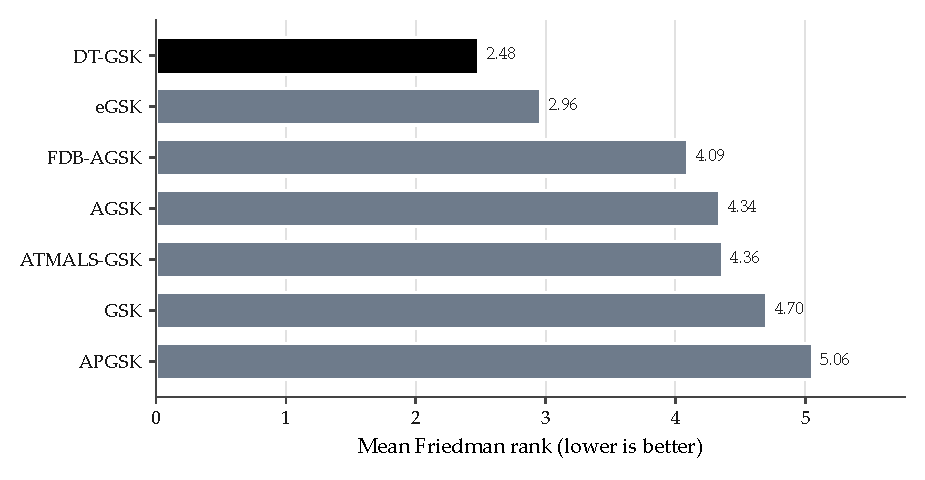
\includegraphics[width=0.72\textwidth]{figures/ranks/friedman_gsk_family}
\caption{Overall (dimension-aggregated) Friedman mean rank of the seven GSK-family
algorithms on CEC2017; lower is better. Same ranks, qualifications, and provenance as
the main paper's family-panel rank table.}\label{fig:supp-overall-ranks}
% BIND: fig friedman_gsk_family.pdf (generate_rank_charts.py; friedman_ranks source)
\end{figure}

\begin{figure}[htbp]
\centering
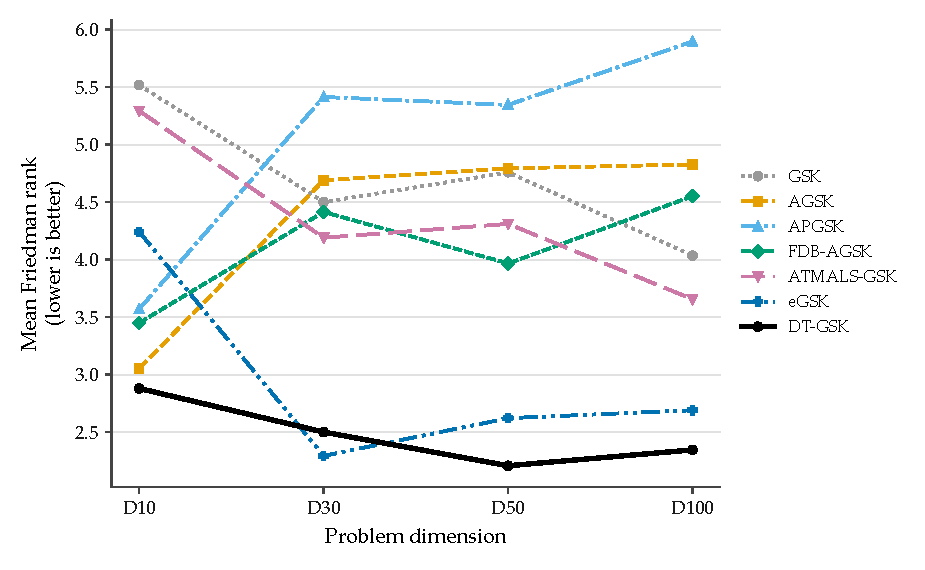
\includegraphics[width=0.82\textwidth]{figures/ranks/rank_vs_dim_cec2017}
\caption{CEC2017 Friedman mean rank against problem dimension
($D\in\{10,30,50,100\}$) for the seven GSK-family algorithms (\dtgsk{} solid
black); the plotted per-dimension values are exactly those of the
main paper's family-panel rank table.}\label{fig:supp-rank-trend}
% BIND: fig rank_vs_dim_cec2017.pdf (generate_rank_charts.py; rank_trend source)
\end{figure}

%==================================================================
\section{Convergence Figure Sets}\label{sec:supp:convergence}
%==================================================================

This section provides the complete convergence record behind the
main-text convergence subset: every scored function of the three suites
whose convergence record this section carries --- CEC2017 at all four
dimensions, CEC2011 at native dimensions, and CEC2013 (bound-constrained)
at the prespecified $D=30$ --- one panel per function, with all 7 panel
algorithms overlaid in every panel.  The CEC2020 and CEC2013LSGO suites
(Sections~S8 and S7) carry no convergence figure set: their releases
promote no curve files, an exclusion recorded in their manifests.
The aggregation basis is identical for all curves in this section: each
curve is the per-checkpoint \emph{mean} across all runs for that
algorithm (51 runs for CEC2017/CEC2013, 25 for CEC2011), with no
smoothing and no interpolation.
% BIND: AN-CONV-2017-D10..D100; AN-CONV-2011-NATIVE; AN-CONV-2013-D30 (P2 aggregation rule)
Axes are log-error with a display-only floor of $10^{-14}$ for exact
zeros; the floor never enters any reported statistic.
% BIND: convergence disclosure logs (cec2017/cec2011/cec2013_missing.log)
Line styles follow a fixed color/linestyle map (Okabe--Ito palette,
\dtgsk{} solid black) with one shared legend per grid, and every panel
carries the full 7/7 series (companion disclosure logs
cec2017\_missing.log, cec2011\_missing.log,
cec2013\_missing.log record zero absences).
% BIND: FIG-CONV-SUP-* validation status (series-count-verified 7/7)

\subsection{CEC2017: All 29 Functions at Each Dimension}\label{sec:supp:conv2017}

Figures~\ref{fig:sconv-cec2017-d10-a}--\ref{fig:sconv-cec2017-d100-d}
cover all 29 CEC2017 functions at each of the four dimensions, split
into four sub-grids per dimension (F1, F3--F9 / F10--F17 / F18--F25 / F26--F30).
For $D = 10$, $30$, and $50$ the \apgsk{} checkpoint evidence derives
from per-generation logs whose producing environment is unrecorded (the
disclosed \apgsk{} evidence limitation); the curves are shown with that
qualification.
% BIND: APGSK-GAP

\begin{figure}[H]
\centering
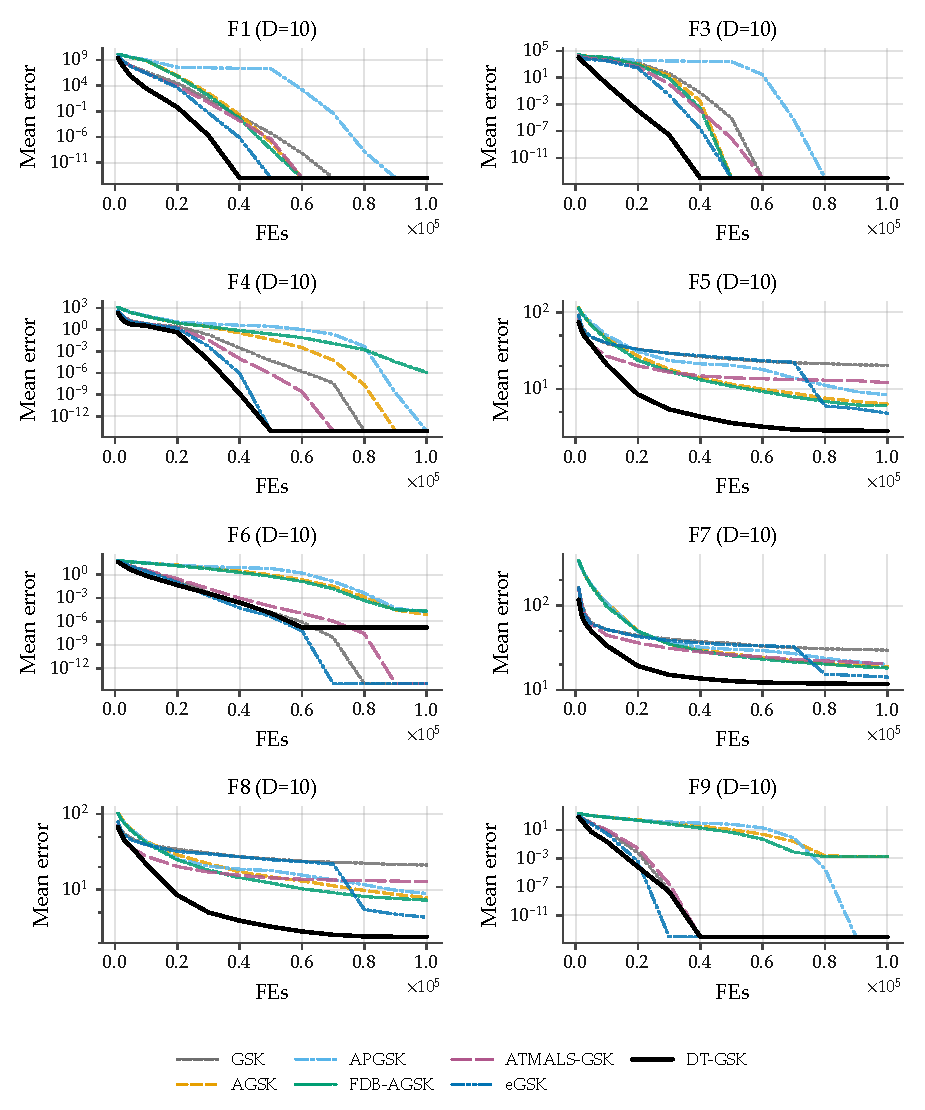
\includegraphics[width=\textwidth,height=0.87\textheight,keepaspectratio]{figures/convergence/all_funcs_D10_a}
\caption{Family-overlay convergence on CEC2017 at $D = 10$, functions
F1, F3--F9 (sub-grid a of 4): per-checkpoint mean error across 51 runs
per algorithm (identical basis for all 7 curves; no smoothing), fixed
Okabe--Ito style map, \dtgsk{} solid black, one shared legend,
log-error $y$-axis with display-only floor $10^{-14}$ for exact zeros.
All panels carry the full 7/7 series.  \apgsk{} checkpoint evidence at this
dimension derives from per-generation logs (disclosed limitation).
}\label{fig:sconv-cec2017-d10-a}
% BIND: FIG-CONV-SUP-2017-D10-A (AN-CONV-2017-D10); APGSK-GAP
\end{figure}

\begin{figure}[H]
\centering
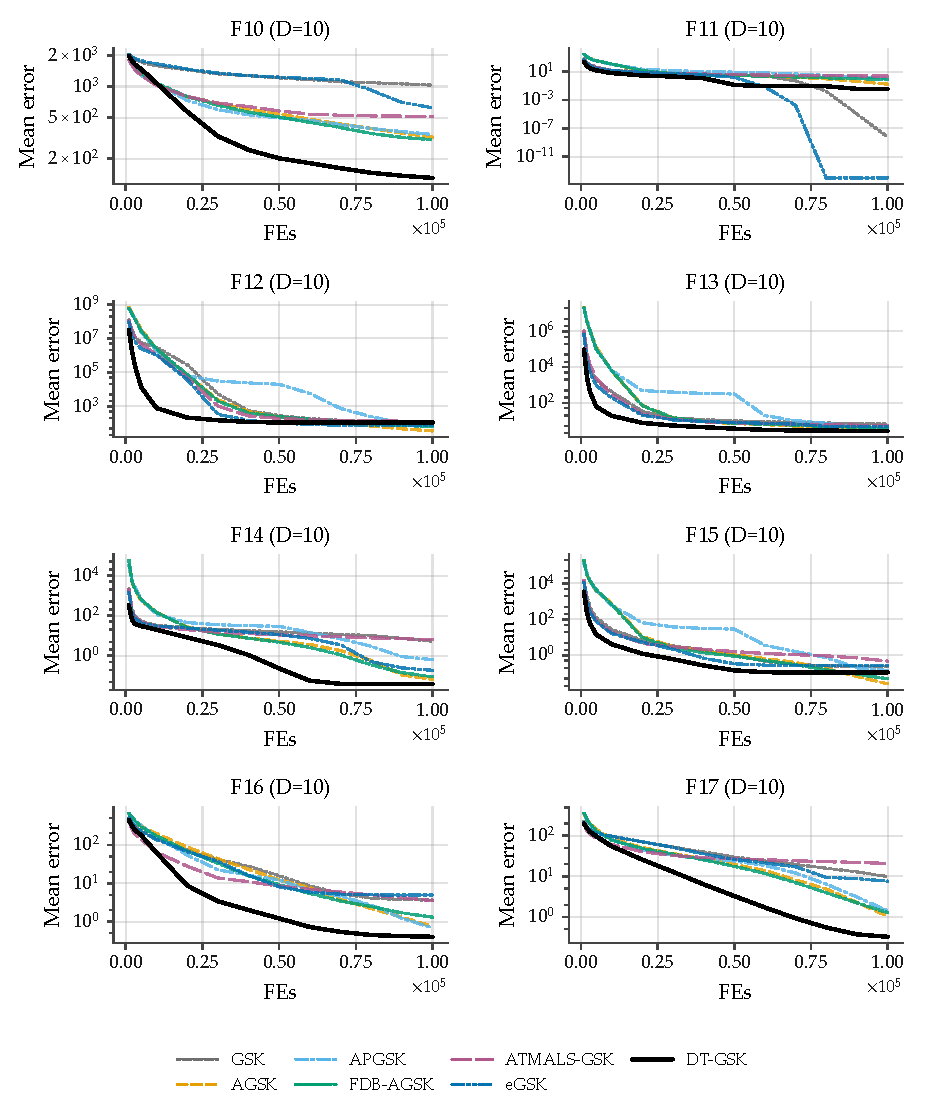
\includegraphics[width=\textwidth,height=0.87\textheight,keepaspectratio]{figures/convergence/all_funcs_D10_b}
\caption{Family-overlay convergence on CEC2017 at $D = 10$, functions
F10--F17 (sub-grid b of 4): per-checkpoint mean error across 51 runs per
algorithm, 7-curve overlay, log-error $y$-axis (display floor
$10^{-14}$), one shared legend.  \apgsk{} checkpoint evidence at this
dimension derives from per-generation logs (disclosed limitation).
}\label{fig:sconv-cec2017-d10-b}
% BIND: FIG-CONV-SUP-2017-D10-B (AN-CONV-2017-D10); APGSK-GAP
\end{figure}

\begin{figure}[H]
\centering
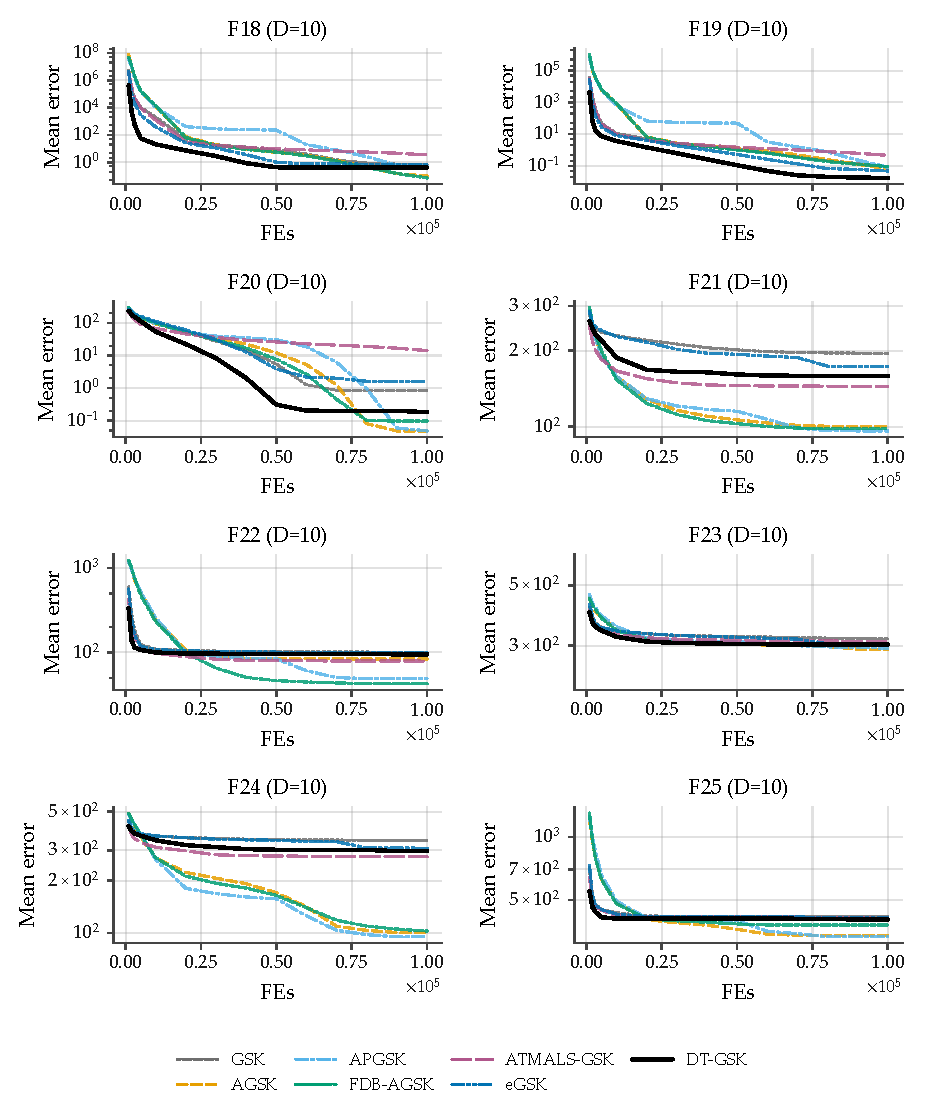
\includegraphics[width=\textwidth,height=0.87\textheight,keepaspectratio]{figures/convergence/all_funcs_D10_c}
\caption{Family-overlay convergence on CEC2017 at $D = 10$, functions
F18--F25 (sub-grid c of 4): per-checkpoint mean error across 51 runs per
algorithm, 7-curve overlay, log-error $y$-axis (display floor
$10^{-14}$), one shared legend.  \apgsk{} checkpoint evidence at this
dimension derives from per-generation logs (disclosed limitation).
}\label{fig:sconv-cec2017-d10-c}
% BIND: FIG-CONV-SUP-2017-D10-C (AN-CONV-2017-D10); APGSK-GAP
\end{figure}

\begin{figure}[H]
\centering
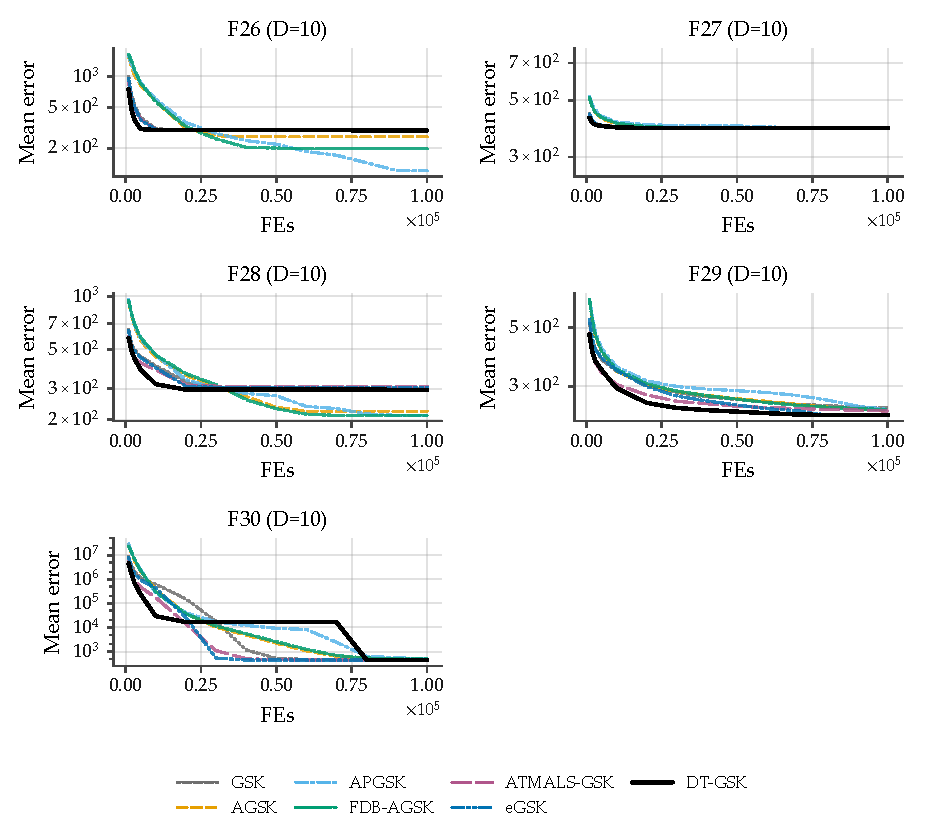
\includegraphics[width=\textwidth,height=0.87\textheight,keepaspectratio]{figures/convergence/all_funcs_D10_d}
\caption{Family-overlay convergence on CEC2017 at $D = 10$, functions
F26--F30 (sub-grid d of 4): per-checkpoint mean error across 51 runs per
algorithm, 7-curve overlay, log-error $y$-axis (display floor
$10^{-14}$), one shared legend.  \apgsk{} checkpoint evidence at this
dimension derives from per-generation logs (disclosed limitation).
}\label{fig:sconv-cec2017-d10-d}
% BIND: FIG-CONV-SUP-2017-D10-D (AN-CONV-2017-D10); APGSK-GAP
\end{figure}

\begin{figure}[H]
\centering
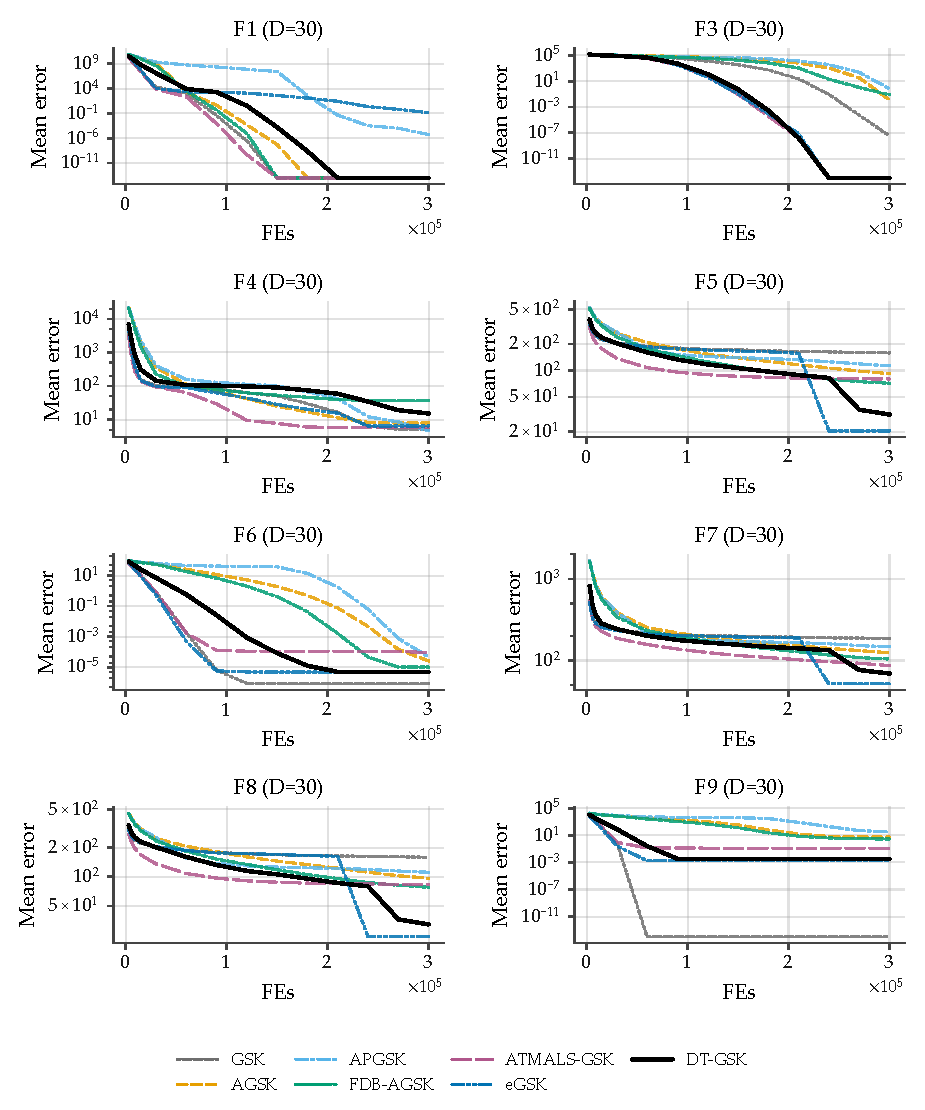
\includegraphics[width=\textwidth,height=0.87\textheight,keepaspectratio]{figures/convergence/all_funcs_D30_a}
\caption{Family-overlay convergence on CEC2017 at $D = 30$, functions
F1, F3--F9 (sub-grid a of 4): per-checkpoint mean error across 51 runs
per algorithm (identical basis for all 7 curves; no smoothing), fixed
Okabe--Ito style map, \dtgsk{} solid black, one shared legend,
log-error $y$-axis with display-only floor $10^{-14}$ for exact zeros.
All panels carry the full 7/7 series.  \apgsk{} checkpoint evidence at this
dimension derives from per-generation logs (disclosed limitation).
}\label{fig:sconv-cec2017-d30-a}
% BIND: FIG-CONV-SUP-2017-D30-A (AN-CONV-2017-D30); APGSK-GAP
\end{figure}

\begin{figure}[H]
\centering
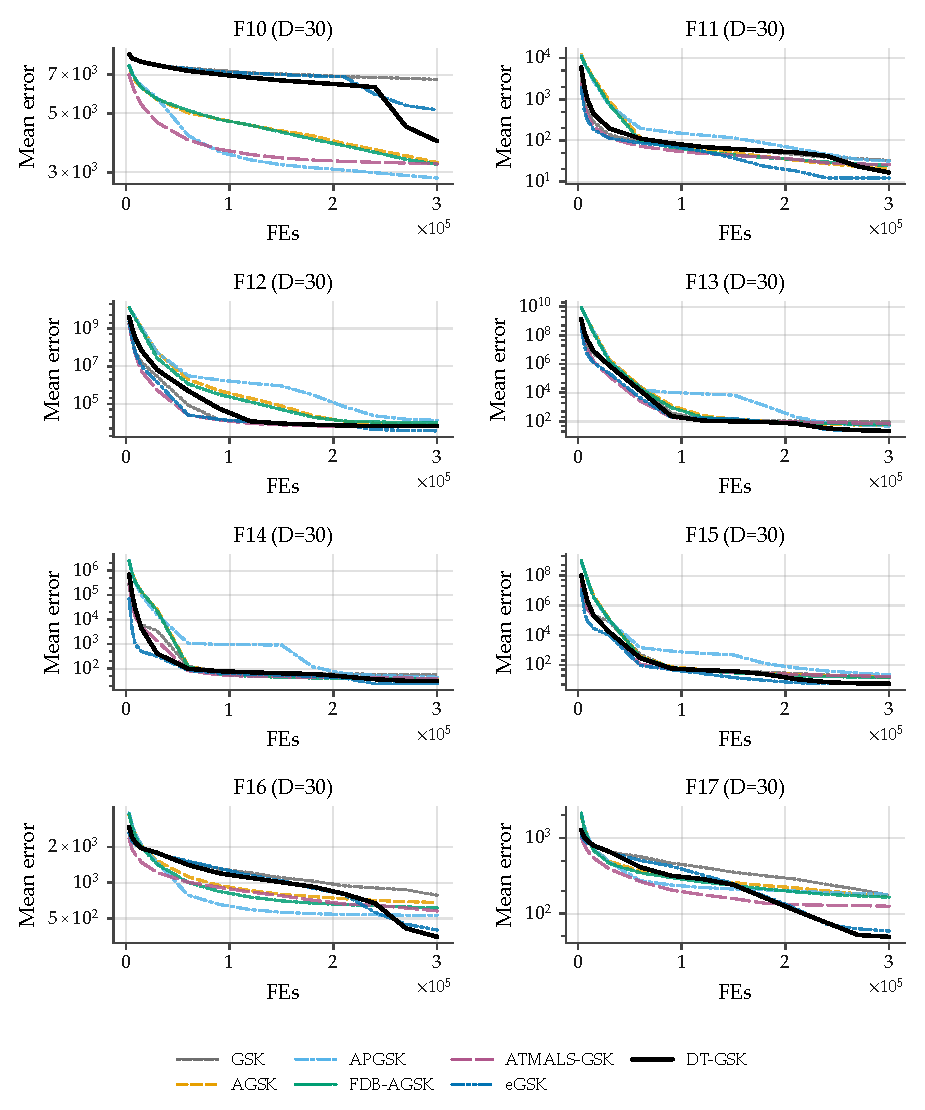
\includegraphics[width=\textwidth,height=0.87\textheight,keepaspectratio]{figures/convergence/all_funcs_D30_b}
\caption{Family-overlay convergence on CEC2017 at $D = 30$, functions
F10--F17 (sub-grid b of 4): per-checkpoint mean error across 51 runs per
algorithm, 7-curve overlay, log-error $y$-axis (display floor
$10^{-14}$), one shared legend.  \apgsk{} checkpoint evidence at this
dimension derives from per-generation logs (disclosed limitation).
}\label{fig:sconv-cec2017-d30-b}
% BIND: FIG-CONV-SUP-2017-D30-B (AN-CONV-2017-D30); APGSK-GAP
\end{figure}

\begin{figure}[H]
\centering
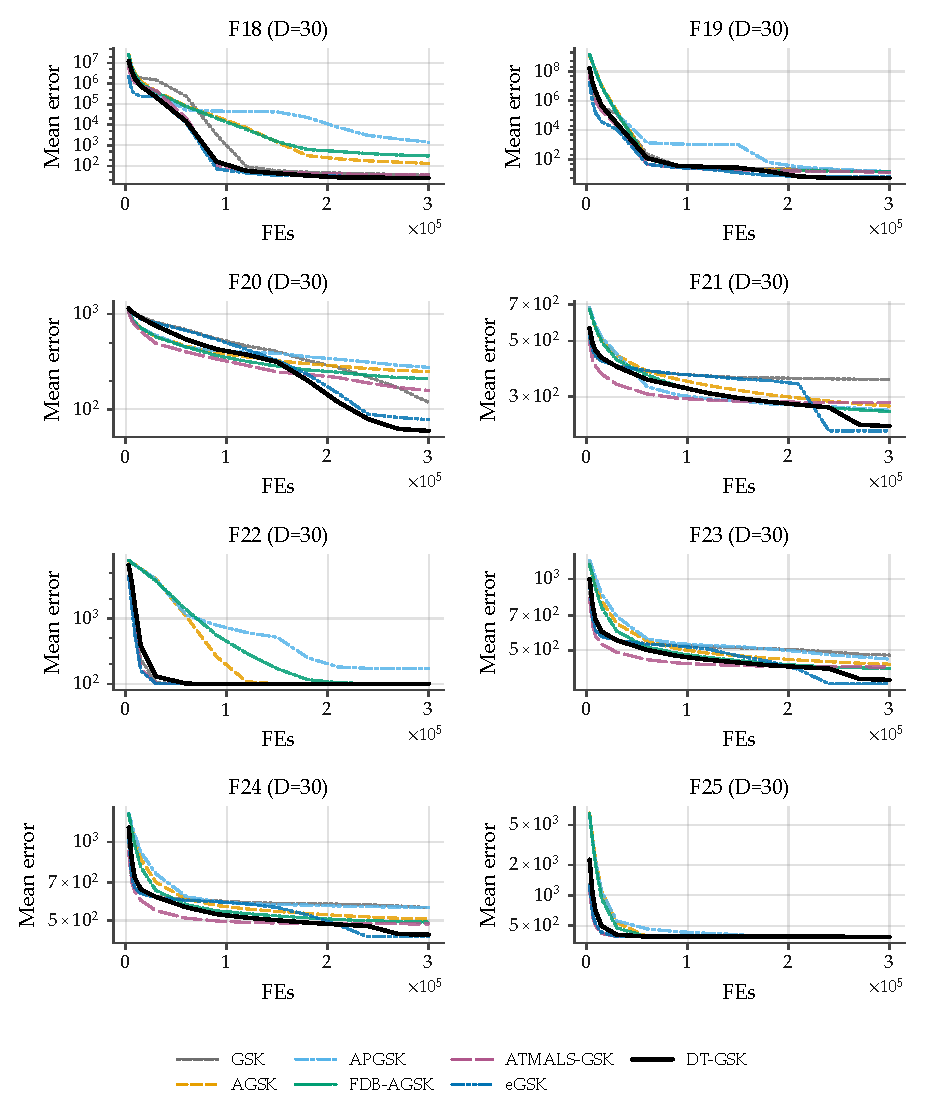
\includegraphics[width=\textwidth,height=0.87\textheight,keepaspectratio]{figures/convergence/all_funcs_D30_c}
\caption{Family-overlay convergence on CEC2017 at $D = 30$, functions
F18--F25 (sub-grid c of 4): per-checkpoint mean error across 51 runs per
algorithm, 7-curve overlay, log-error $y$-axis (display floor
$10^{-14}$), one shared legend.  \apgsk{} checkpoint evidence at this
dimension derives from per-generation logs (disclosed limitation).
}\label{fig:sconv-cec2017-d30-c}
% BIND: FIG-CONV-SUP-2017-D30-C (AN-CONV-2017-D30); APGSK-GAP
\end{figure}

\begin{figure}[H]
\centering
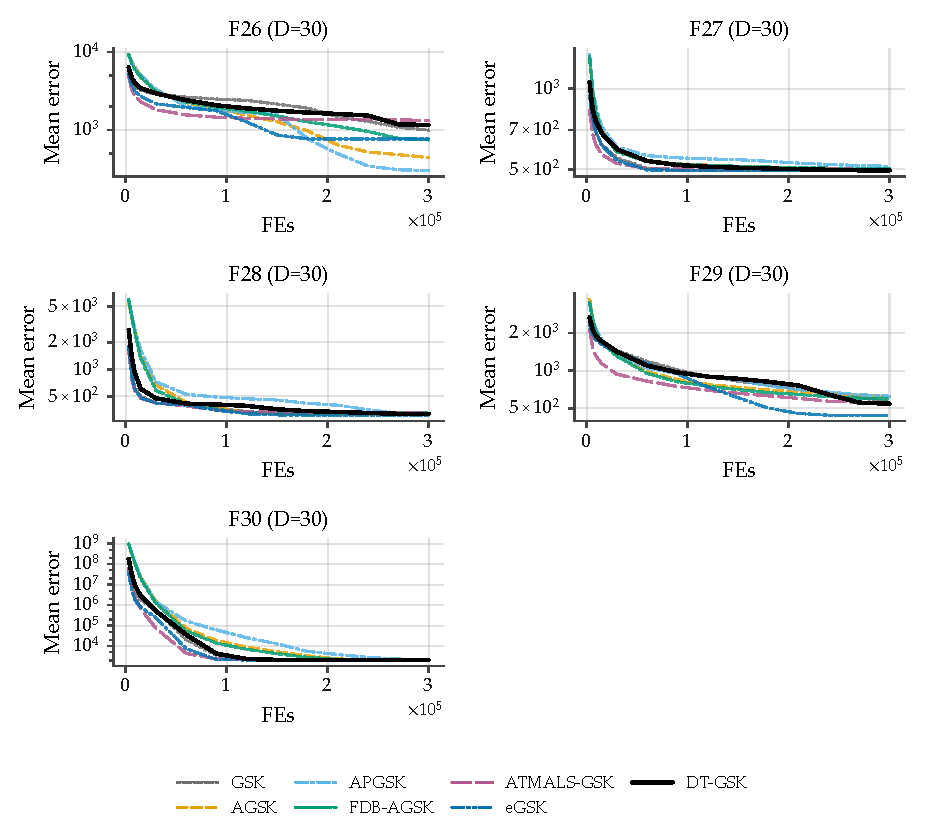
\includegraphics[width=\textwidth,height=0.87\textheight,keepaspectratio]{figures/convergence/all_funcs_D30_d}
\caption{Family-overlay convergence on CEC2017 at $D = 30$, functions
F26--F30 (sub-grid d of 4): per-checkpoint mean error across 51 runs per
algorithm, 7-curve overlay, log-error $y$-axis (display floor
$10^{-14}$), one shared legend.  \apgsk{} checkpoint evidence at this
dimension derives from per-generation logs (disclosed limitation).
}\label{fig:sconv-cec2017-d30-d}
% BIND: FIG-CONV-SUP-2017-D30-D (AN-CONV-2017-D30); APGSK-GAP
\end{figure}

\begin{figure}[H]
\centering
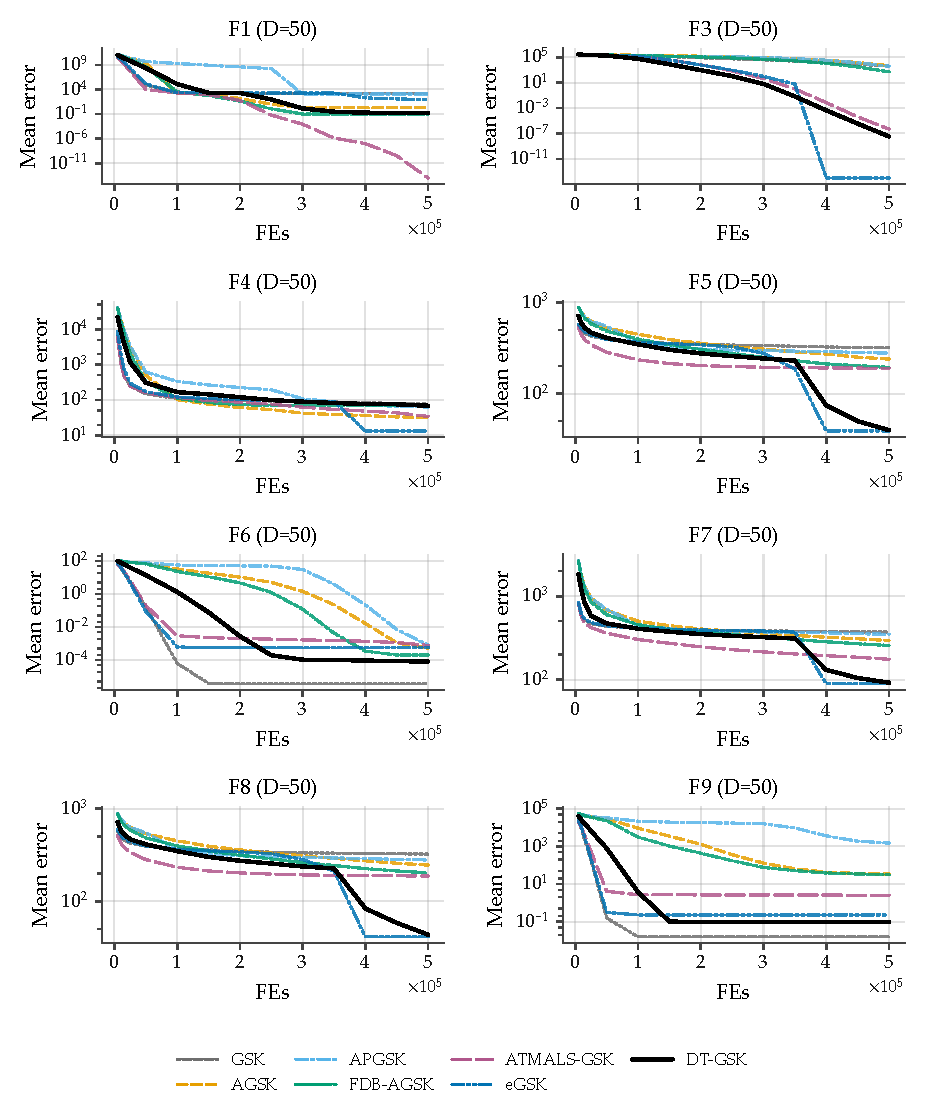
\includegraphics[width=\textwidth,height=0.87\textheight,keepaspectratio]{figures/convergence/all_funcs_D50_a}
\caption{Family-overlay convergence on CEC2017 at $D = 50$, functions
F1, F3--F9 (sub-grid a of 4): per-checkpoint mean error across 51 runs
per algorithm (identical basis for all 7 curves; no smoothing), fixed
Okabe--Ito style map, \dtgsk{} solid black, one shared legend,
log-error $y$-axis with display-only floor $10^{-14}$ for exact zeros.
All panels carry the full 7/7 series.  \apgsk{} checkpoint evidence at this
dimension derives from per-generation logs (disclosed limitation).
}\label{fig:sconv-cec2017-d50-a}
% BIND: FIG-CONV-SUP-2017-D50-A (AN-CONV-2017-D50); APGSK-GAP
\end{figure}

\begin{figure}[H]
\centering
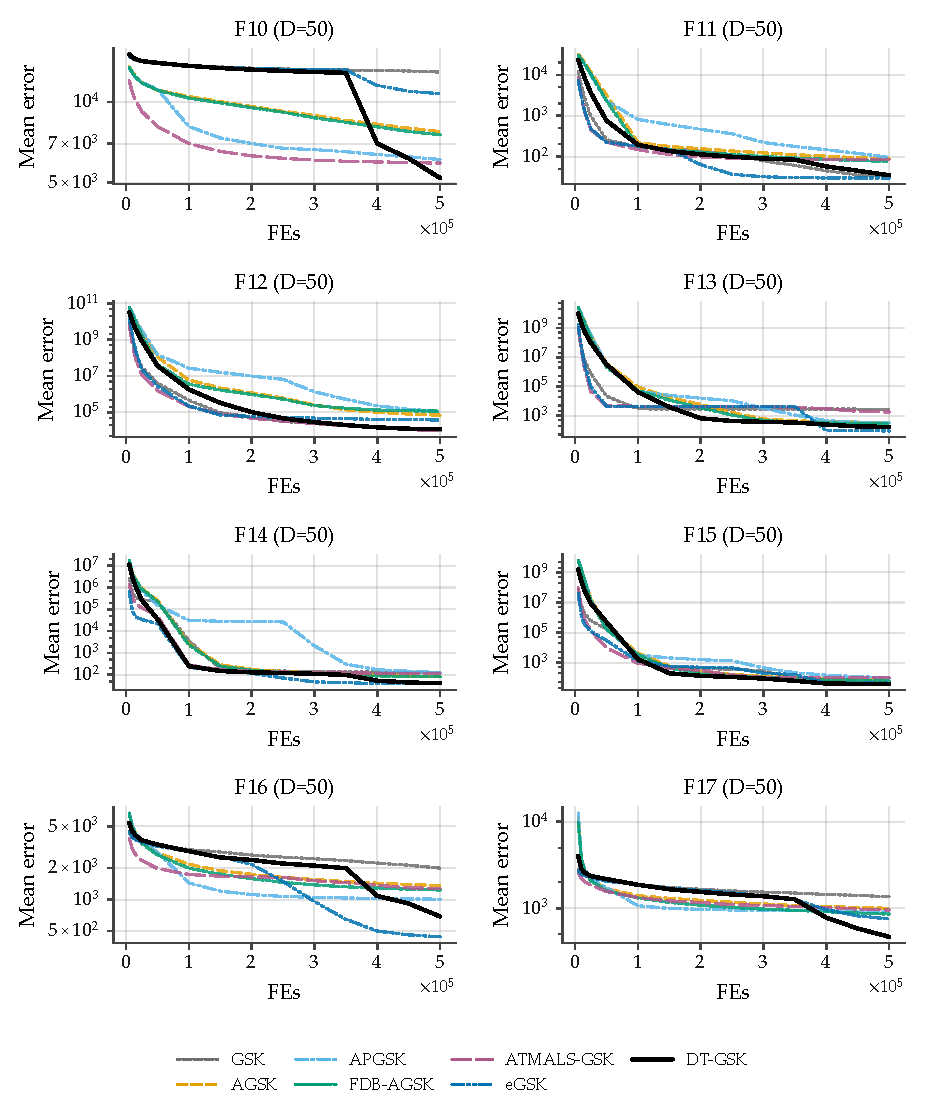
\includegraphics[width=\textwidth,height=0.87\textheight,keepaspectratio]{figures/convergence/all_funcs_D50_b}
\caption{Family-overlay convergence on CEC2017 at $D = 50$, functions
F10--F17 (sub-grid b of 4): per-checkpoint mean error across 51 runs per
algorithm, 7-curve overlay, log-error $y$-axis (display floor
$10^{-14}$), one shared legend.  \apgsk{} checkpoint evidence at this
dimension derives from per-generation logs (disclosed limitation).
}\label{fig:sconv-cec2017-d50-b}
% BIND: FIG-CONV-SUP-2017-D50-B (AN-CONV-2017-D50); APGSK-GAP
\end{figure}

\begin{figure}[H]
\centering
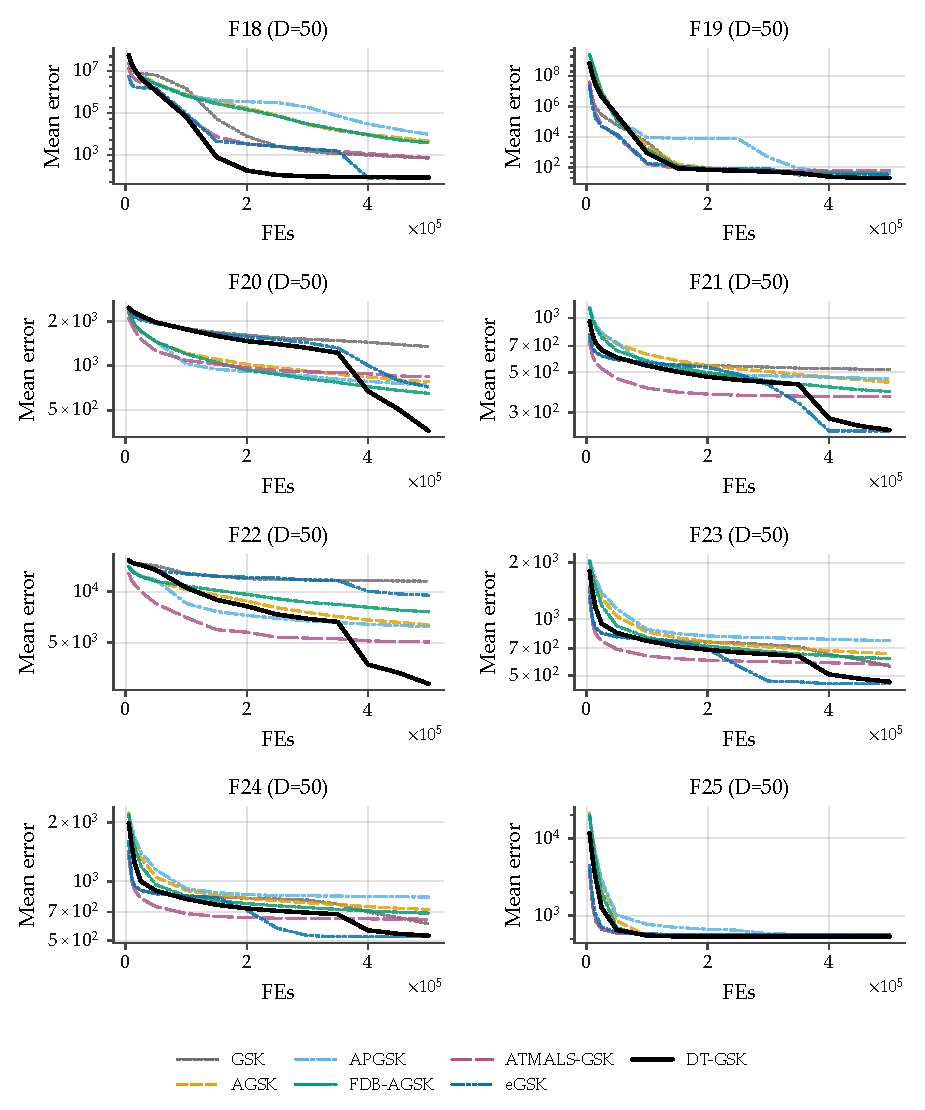
\includegraphics[width=\textwidth,height=0.87\textheight,keepaspectratio]{figures/convergence/all_funcs_D50_c}
\caption{Family-overlay convergence on CEC2017 at $D = 50$, functions
F18--F25 (sub-grid c of 4): per-checkpoint mean error across 51 runs per
algorithm, 7-curve overlay, log-error $y$-axis (display floor
$10^{-14}$), one shared legend.  \apgsk{} checkpoint evidence at this
dimension derives from per-generation logs (disclosed limitation).
}\label{fig:sconv-cec2017-d50-c}
% BIND: FIG-CONV-SUP-2017-D50-C (AN-CONV-2017-D50); APGSK-GAP
\end{figure}

\begin{figure}[H]
\centering
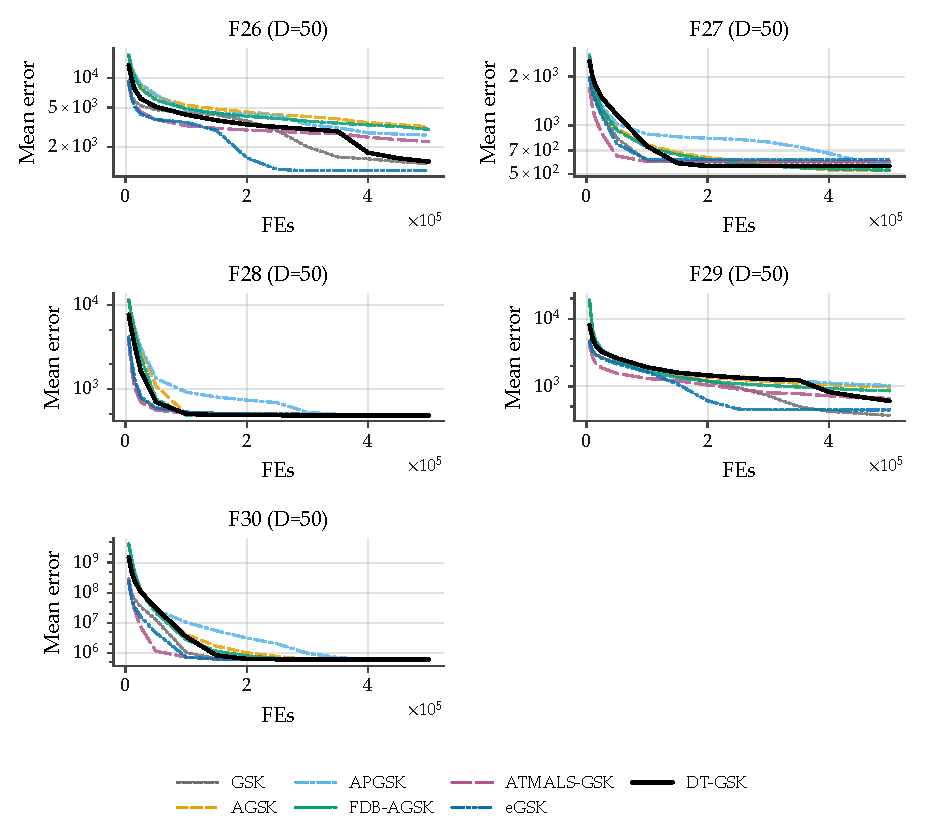
\includegraphics[width=\textwidth,height=0.87\textheight,keepaspectratio]{figures/convergence/all_funcs_D50_d}
\caption{Family-overlay convergence on CEC2017 at $D = 50$, functions
F26--F30 (sub-grid d of 4): per-checkpoint mean error across 51 runs per
algorithm, 7-curve overlay, log-error $y$-axis (display floor
$10^{-14}$), one shared legend.  \apgsk{} checkpoint evidence at this
dimension derives from per-generation logs (disclosed limitation).
}\label{fig:sconv-cec2017-d50-d}
% BIND: FIG-CONV-SUP-2017-D50-D (AN-CONV-2017-D50); APGSK-GAP
\end{figure}

\begin{figure}[H]
\centering
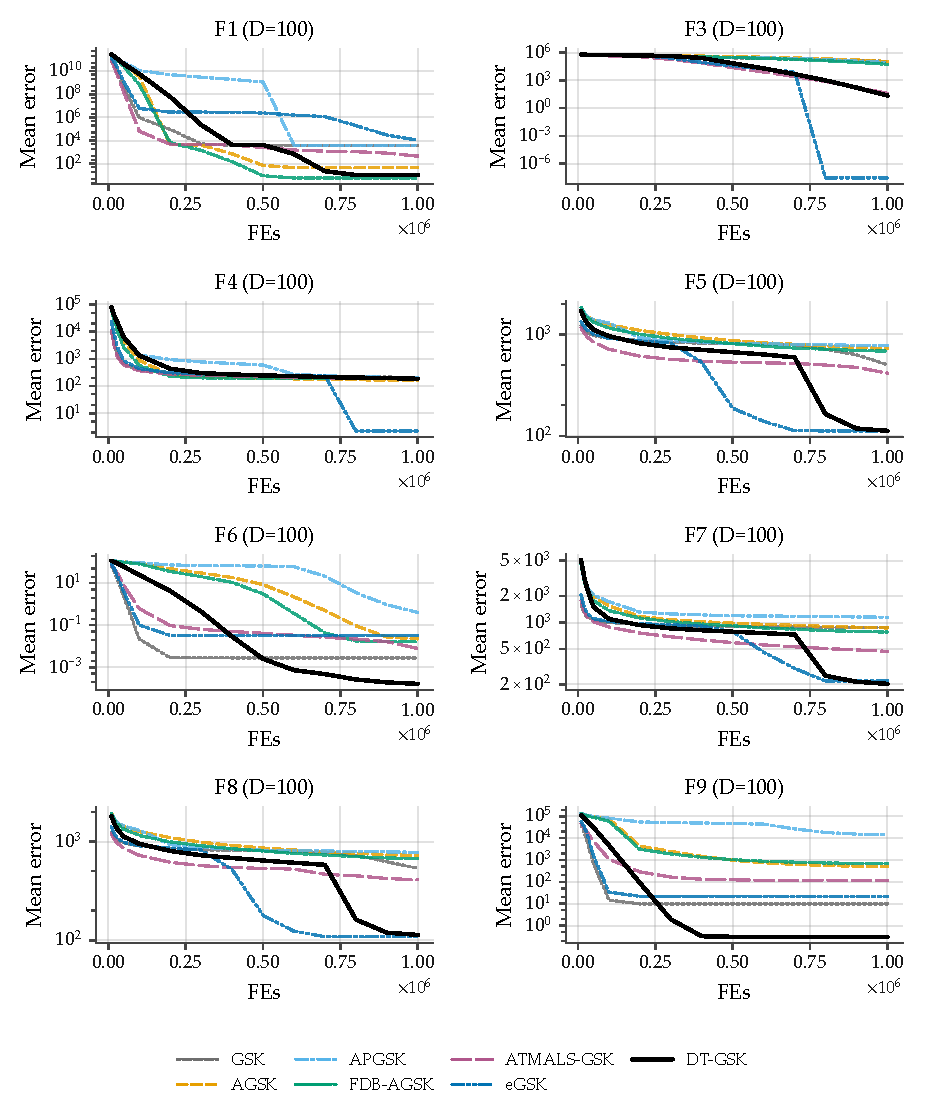
\includegraphics[width=\textwidth,height=0.87\textheight,keepaspectratio]{figures/convergence/all_funcs_D100_a}
\caption{Family-overlay convergence on CEC2017 at $D = 100$, functions
F1, F3--F9 (sub-grid a of 4): per-checkpoint mean error across 51 runs
per algorithm (identical basis for all 7 curves; no smoothing), fixed
Okabe--Ito style map, \dtgsk{} solid black, one shared legend,
log-error $y$-axis with display-only floor $10^{-14}$ for exact zeros.
All panels carry the full 7/7 series.  \apgsk{} checkpoint evidence at this
dimension derives from per-generation logs (disclosed limitation).
}\label{fig:sconv-cec2017-d100-a}
% BIND: FIG-CONV-SUP-2017-D100-A (AN-CONV-2017-D100); APGSK-GAP
\end{figure}

\begin{figure}[H]
\centering
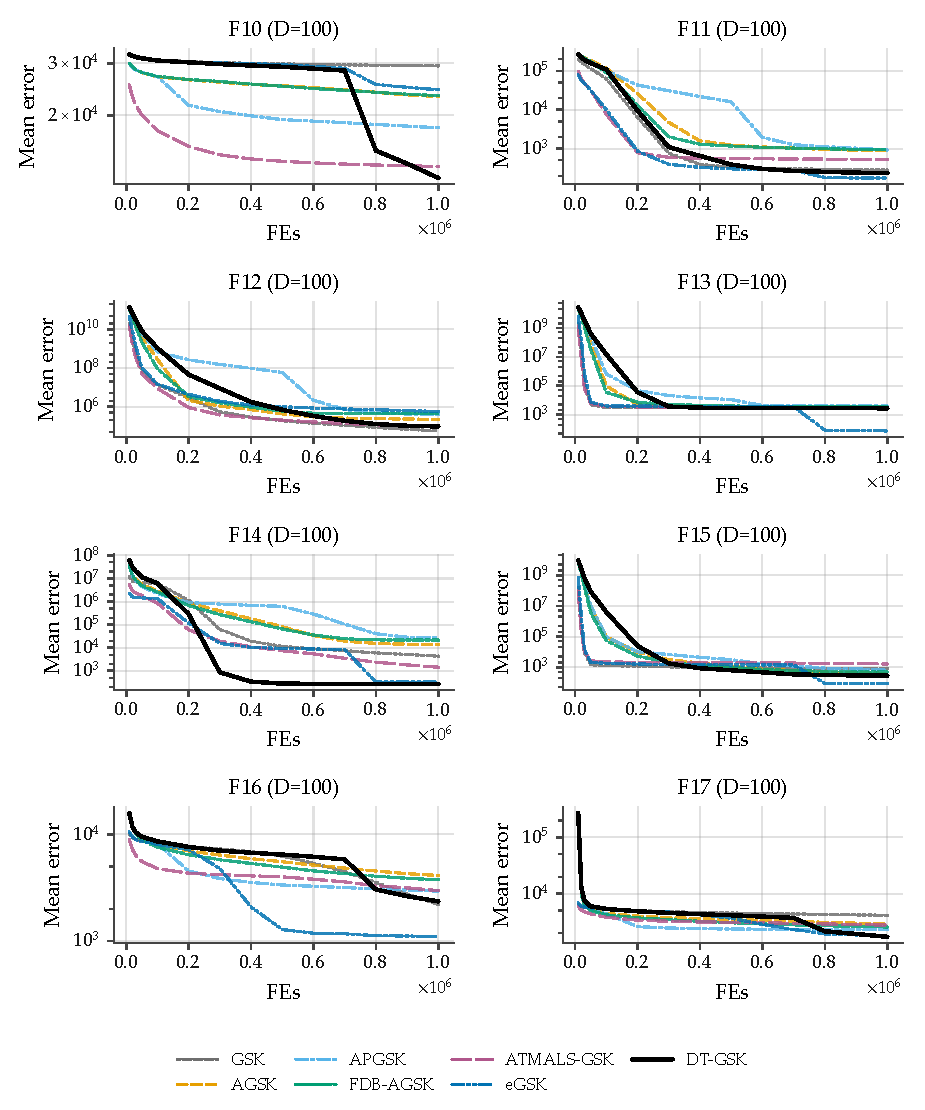
\includegraphics[width=\textwidth,height=0.87\textheight,keepaspectratio]{figures/convergence/all_funcs_D100_b}
\caption{Family-overlay convergence on CEC2017 at $D = 100$, functions
F10--F17 (sub-grid b of 4): per-checkpoint mean error across 51 runs per
algorithm, 7-curve overlay, log-error $y$-axis (display floor
$10^{-14}$), one shared legend.  \apgsk{} checkpoint evidence at this
dimension derives from per-generation logs (disclosed limitation).
}\label{fig:sconv-cec2017-d100-b}
% BIND: FIG-CONV-SUP-2017-D100-B (AN-CONV-2017-D100); APGSK-GAP
\end{figure}

\begin{figure}[H]
\centering
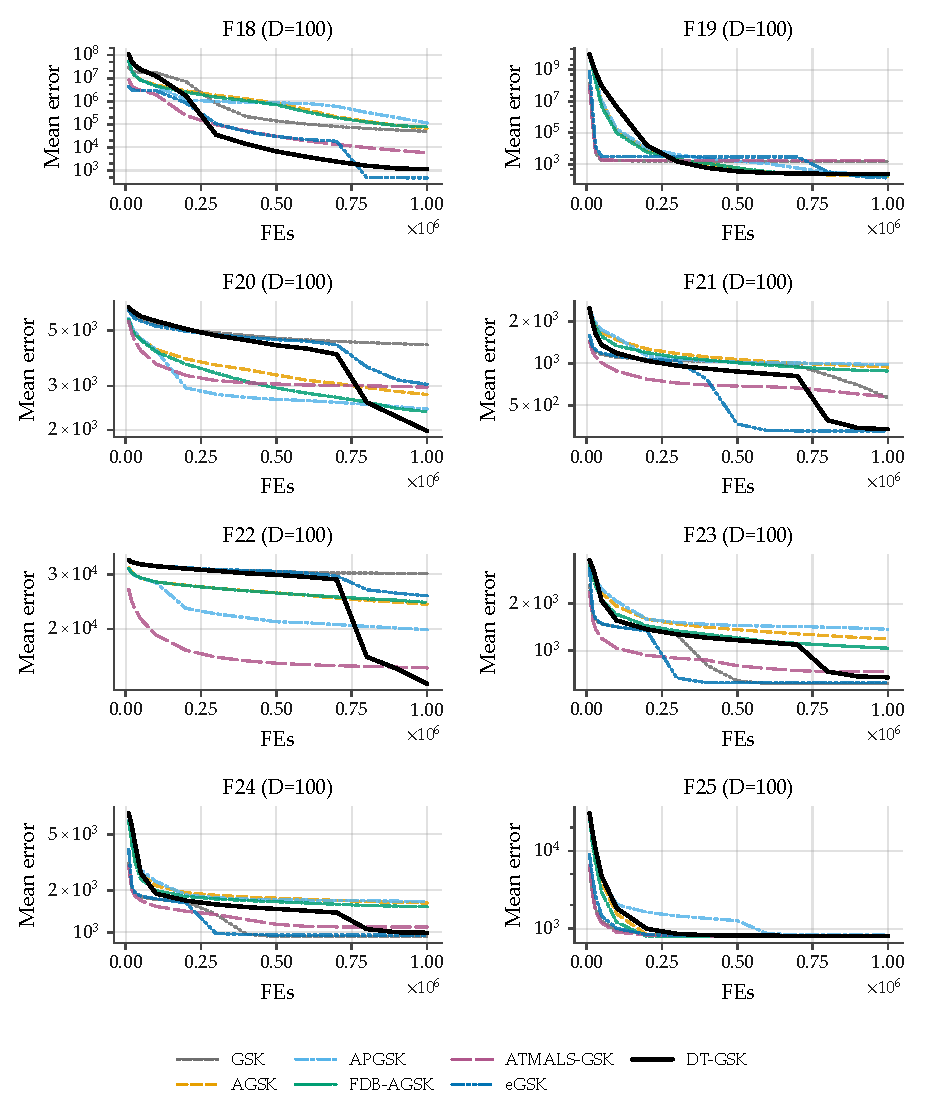
\includegraphics[width=\textwidth,height=0.87\textheight,keepaspectratio]{figures/convergence/all_funcs_D100_c}
\caption{Family-overlay convergence on CEC2017 at $D = 100$, functions
F18--F25 (sub-grid c of 4): per-checkpoint mean error across 51 runs per
algorithm, 7-curve overlay, log-error $y$-axis (display floor
$10^{-14}$), one shared legend.  \apgsk{} checkpoint evidence at this
dimension derives from per-generation logs (disclosed limitation).
}\label{fig:sconv-cec2017-d100-c}
% BIND: FIG-CONV-SUP-2017-D100-C (AN-CONV-2017-D100); APGSK-GAP
\end{figure}

\begin{figure}[H]
\centering
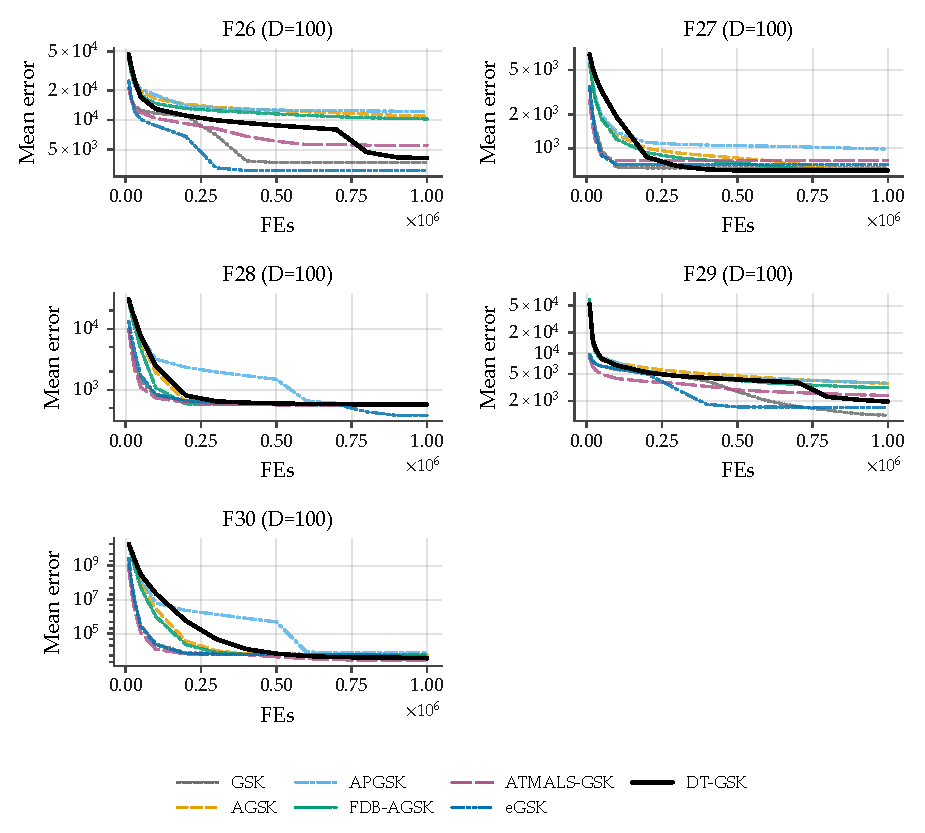
\includegraphics[width=\textwidth,height=0.87\textheight,keepaspectratio]{figures/convergence/all_funcs_D100_d}
\caption{Family-overlay convergence on CEC2017 at $D = 100$, functions
F26--F30 (sub-grid d of 4): per-checkpoint mean error across 51 runs per
algorithm, 7-curve overlay, log $y$-axis (display floor
$10^{-14}$), one shared legend.  \apgsk{} checkpoint evidence at this
dimension derives from per-generation logs (disclosed limitation).
}\label{fig:sconv-cec2017-d100-d}
% BIND: FIG-CONV-SUP-2017-D100-D (AN-CONV-2017-D100); APGSK-GAP
\end{figure}

\subsection{CEC2011: All 22 Real-World Problems}\label{sec:supp:conv2011}

Figures~\ref{fig:sconv-cec2011-a}--\ref{fig:sconv-cec2011-c} cover all
22 CEC2011 real-world problems at their native dimensions, split into
three sub-grids (problems P1--P8 / P9--P16 / P17--P22; each panel is
titled by the suite's function identifier and native dimension).
Because several CEC2011 problems have negative optima, the plotted
quantity is the per-checkpoint mean of the \emph{raw best objective}
across 25 runs, and four panels whose means are negative fall back from
the log axis to a linear $y$-axis with an in-panel disclosure: P2, P5,
and P6 in sub-grid a, and P10 in sub-grid b; all other panels use the
log axis with display floor $10^{-14}$.
% BIND: FIG-CONV-CEC2011-A/B/C (AN-CONV-2011-NATIVE); linear-fallback count per figure_qa (a=3 [F2,F5,F6], b=1 [F10], c=0)
Outcome context for this suite (disclosed alongside the figures, not
after them): within the family panel, \dtgsk{}'s across-problem
Wilcoxon versus \egsk{} on CEC2011 is a statistically significant loss
($n = 22$, Holm-corrected $p = 4.2 \times 10^{-2}$).
% BIND: CEC2011-EGSK-LOSS (AN-PW-2011-NATIVE)

\begin{figure}[H]
\centering
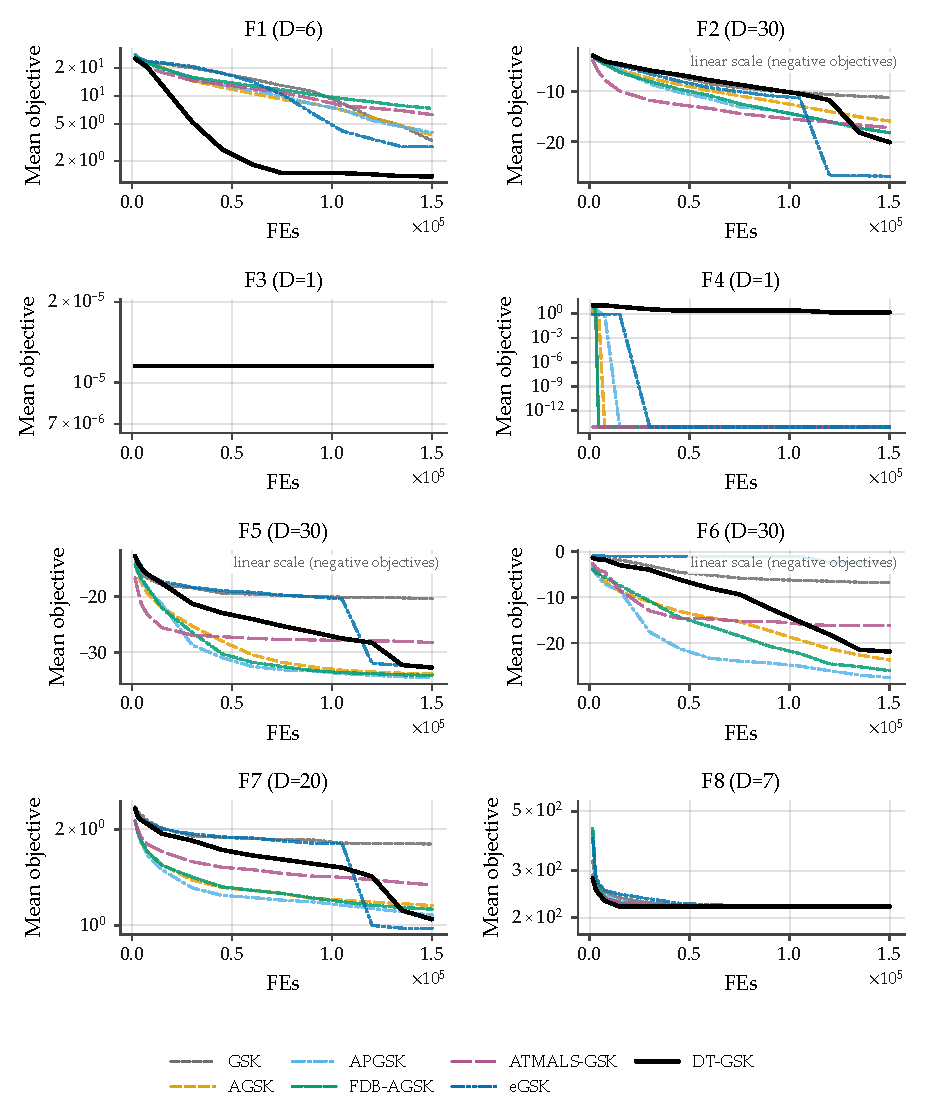
\includegraphics[width=\textwidth,height=0.87\textheight,keepaspectratio]{figures/convergence/cec2011_a}
\caption{Family-overlay convergence on the CEC2011 real-world optimization benchmark suite,
problems P1--P8 at native dimensions (sub-grid a of 3): per-checkpoint
mean of the raw best objective across 25 runs per algorithm, 7-curve
overlay, one shared legend.  The three panels with negative means (P2,
P5, P6) fall back to a linear $y$-axis with an in-panel disclosure; all
other panels use the log axis with display floor $10^{-14}$.  All
panels carry 7/7 series.  Suite-level outcome context: \dtgsk{}
significantly loses to \egsk{} across problems on this suite
(Holm-corrected $p = 4.2 \times 10^{-2}$).  }\label{fig:sconv-cec2011-a}
% BIND: FIG-CONV-CEC2011-A (AN-CONV-2011-NATIVE); CEC2011-EGSK-LOSS
\end{figure}

\begin{figure}[H]
\centering
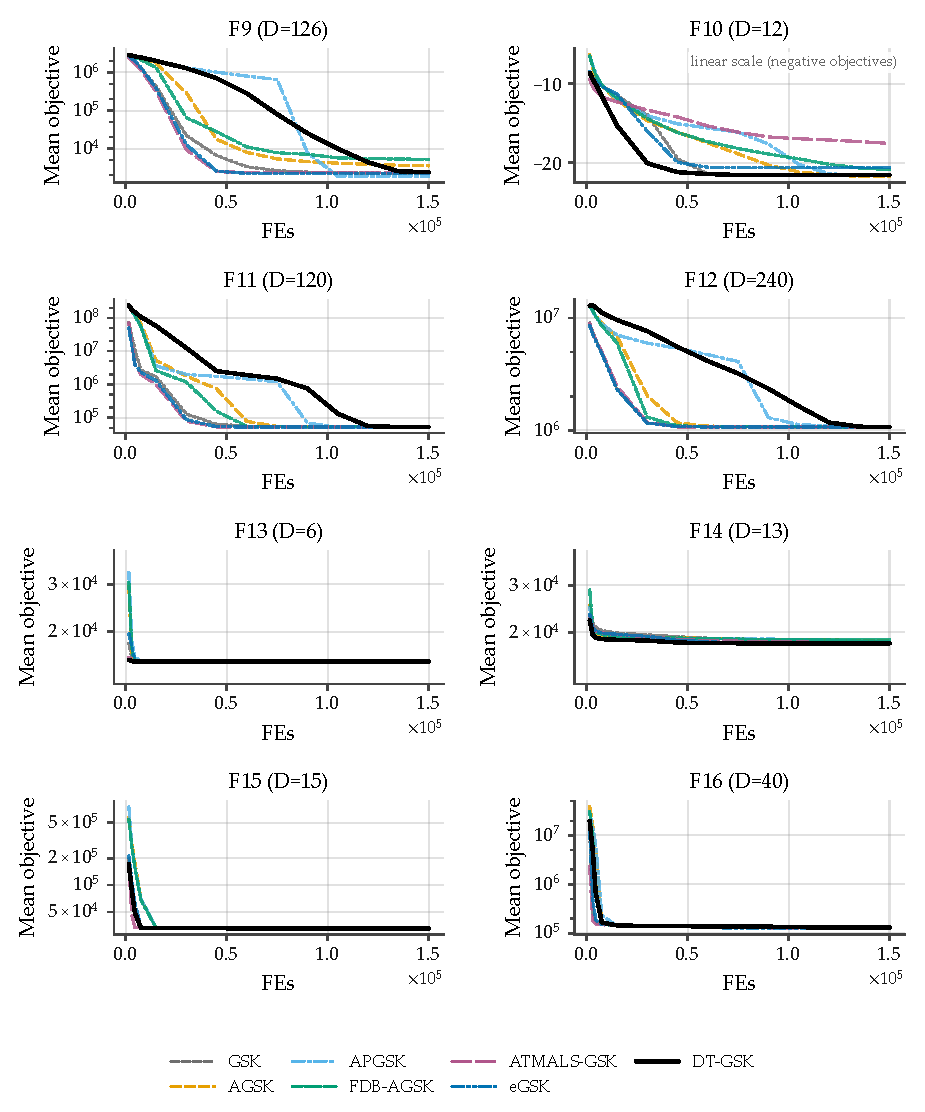
\includegraphics[width=\textwidth,height=0.87\textheight,keepaspectratio]{figures/convergence/cec2011_b}
\caption{Family-overlay convergence on the CEC2011 real-world optimization benchmark suite,
problems P9--P16 at native dimensions (sub-grid b of 3): per-checkpoint
mean of the raw best objective across 25 runs per algorithm, 7-curve
overlay, one shared legend.  The panel with negative means (P10) falls
back to a linear $y$-axis with an in-panel disclosure; all other panels
use the log axis with display floor $10^{-14}$.  All panels carry 7/7
series.  Suite-level outcome context: \dtgsk{} significantly loses to
\egsk{} across problems on this suite (Holm-corrected
$p = 4.2 \times 10^{-2}$).  }\label{fig:sconv-cec2011-b}
% BIND: FIG-CONV-CEC2011-B (AN-CONV-2011-NATIVE); CEC2011-EGSK-LOSS
\end{figure}

\begin{figure}[H]
\centering
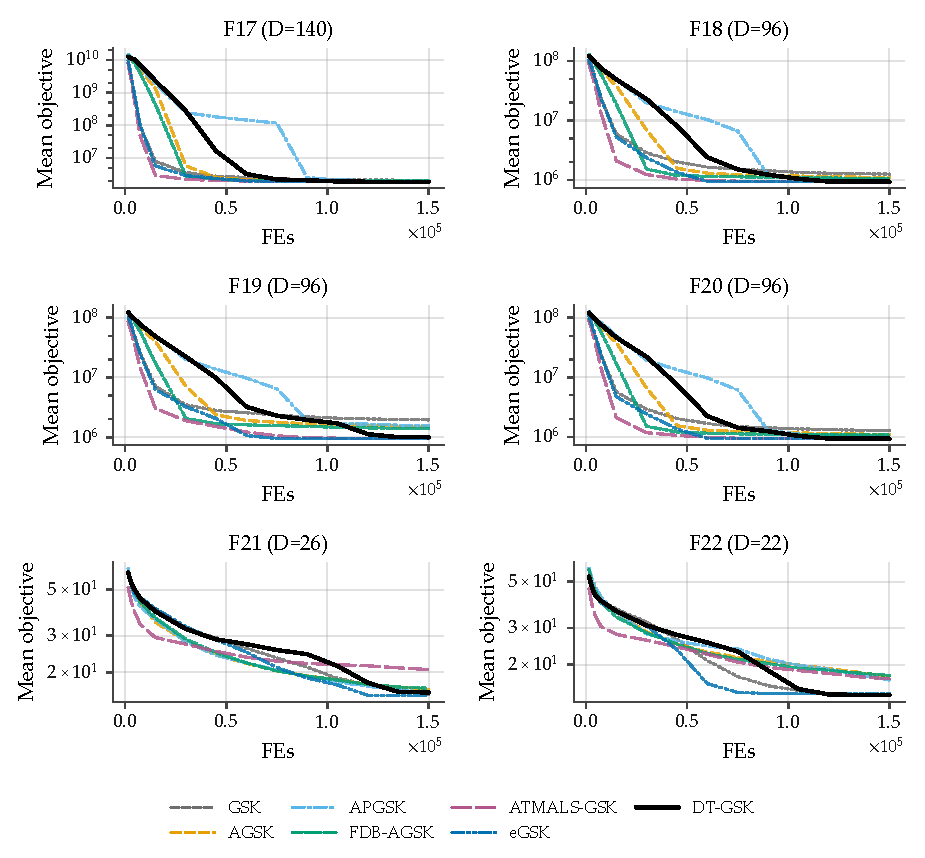
\includegraphics[width=\textwidth,height=0.87\textheight,keepaspectratio]{figures/convergence/cec2011_c}
\caption{Family-overlay convergence on the CEC2011 real-world optimization benchmark suite,
problems P17--P22 at native dimensions (sub-grid c of 3): per-checkpoint
mean of the raw best objective across 25 runs per algorithm, 7-curve
overlay, log-error $y$-axis with display floor $10^{-14}$, one shared
legend.  All panels carry 7/7 series.  Suite-level outcome context:
\dtgsk{} significantly loses to \egsk{} across problems on this suite
(Holm-corrected $p = 4.2 \times 10^{-2}$).  }\label{fig:sconv-cec2011-c}
% BIND: FIG-CONV-CEC2011-C (AN-CONV-2011-NATIVE); CEC2011-EGSK-LOSS
\end{figure}

\subsection{CEC2013 Second Comparison Suite: All 28 Functions at $D = 30$}\label{sec:supp:conv2013}

Figures~\ref{fig:sconv-cec2013-d30-a}--\ref{fig:sconv-cec2013-d30-d}
cover all 28 functions of the CEC2013 second comparison suite at
$D = 30$ --- the only prespecified CEC2013 convergence dimension ---
split into four sub-grids (F1--F8 / F9--F16 / F17--F24 / F25--F28).
% BIND: FIG-CONV-CEC2013-D30-A..D (AN-CONV-2013-D30; prespecification P4)
The panel-level outcome disclosure for this suite and dimension applies
here as in Section~\ref{sec:supp:cec2013}: \dtgsk{} places third by
Friedman mean rank at $D = 30$, behind \egsk{} and \atmals{}.
% BIND: CEC2013-D30-THIRD (AN-OMNI-2013-D30)

\begin{figure}[H]
\centering
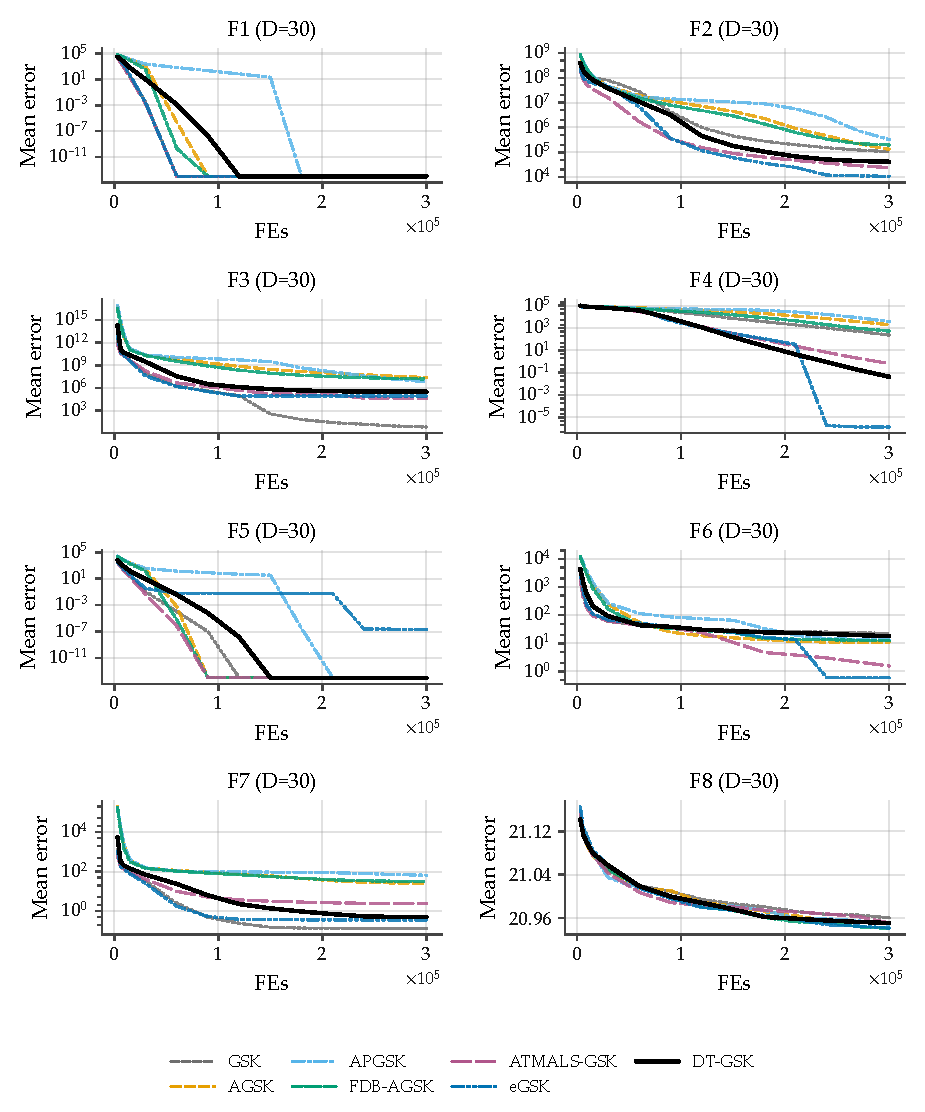
\includegraphics[width=\textwidth,height=0.87\textheight,keepaspectratio]{figures/convergence/cec2013_a}
\caption{Family-overlay convergence on the CEC2013 second comparison
suite at $D = 30$, functions F1--F8 (sub-grid a of 4): per-checkpoint
mean error across 51 runs per algorithm, 7-curve overlay, log-error
$y$-axis (display floor $10^{-14}$), one shared legend.  All panels
carry 7/7 series.  Panel-level context at this dimension: \dtgsk{}
places third by Friedman mean rank behind \egsk{} and \atmals{}.
}\label{fig:sconv-cec2013-d30-a}
% BIND: FIG-CONV-CEC2013-D30-A (AN-CONV-2013-D30); CEC2013-D30-THIRD
\end{figure}

\begin{figure}[H]
\centering
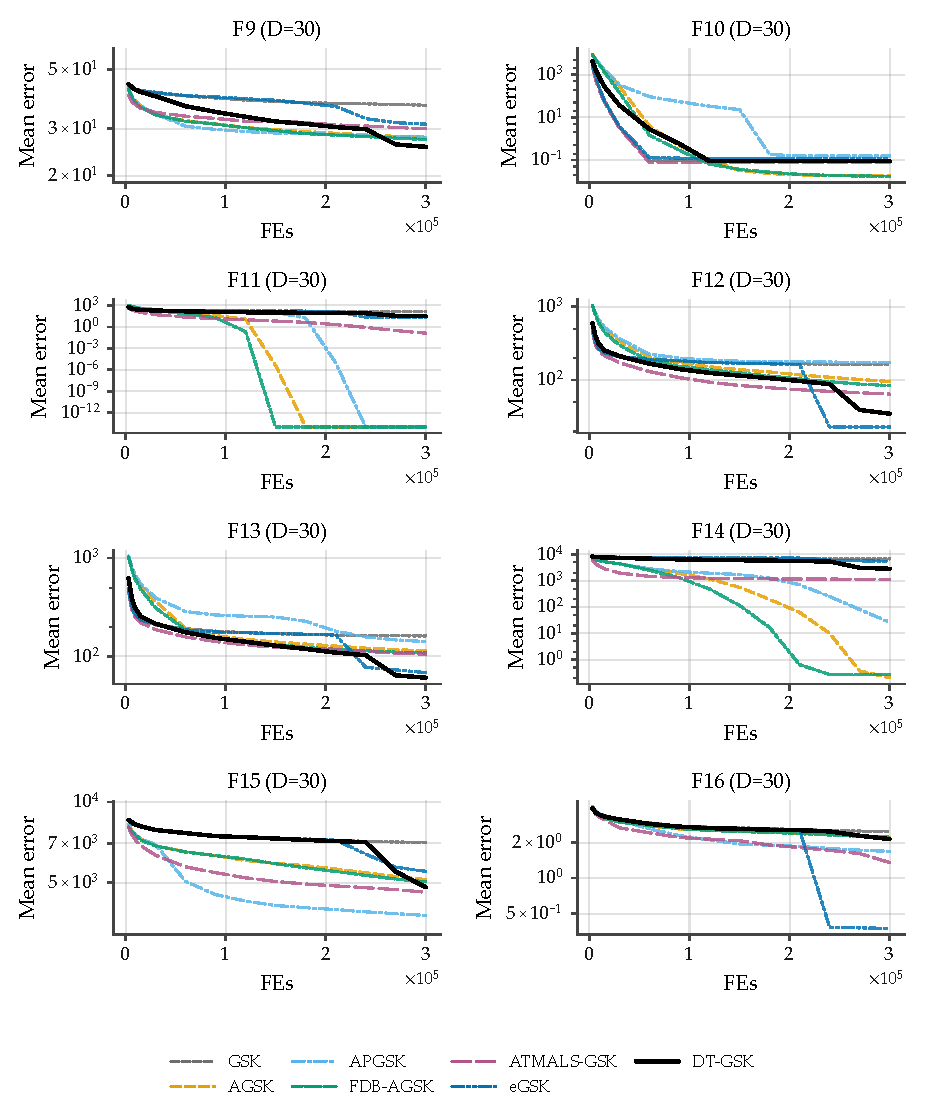
\includegraphics[width=\textwidth,height=0.87\textheight,keepaspectratio]{figures/convergence/cec2013_b}
\caption{Family-overlay convergence on the CEC2013 second comparison
suite at $D = 30$, functions F9--F16 (sub-grid b of 4): per-checkpoint
mean error across 51 runs per algorithm, 7-curve overlay, log-error
$y$-axis (display floor $10^{-14}$), one shared legend.  All panels
carry 7/7 series.  }\label{fig:sconv-cec2013-d30-b}
% BIND: FIG-CONV-CEC2013-D30-B (AN-CONV-2013-D30)
\end{figure}

\begin{figure}[H]
\centering
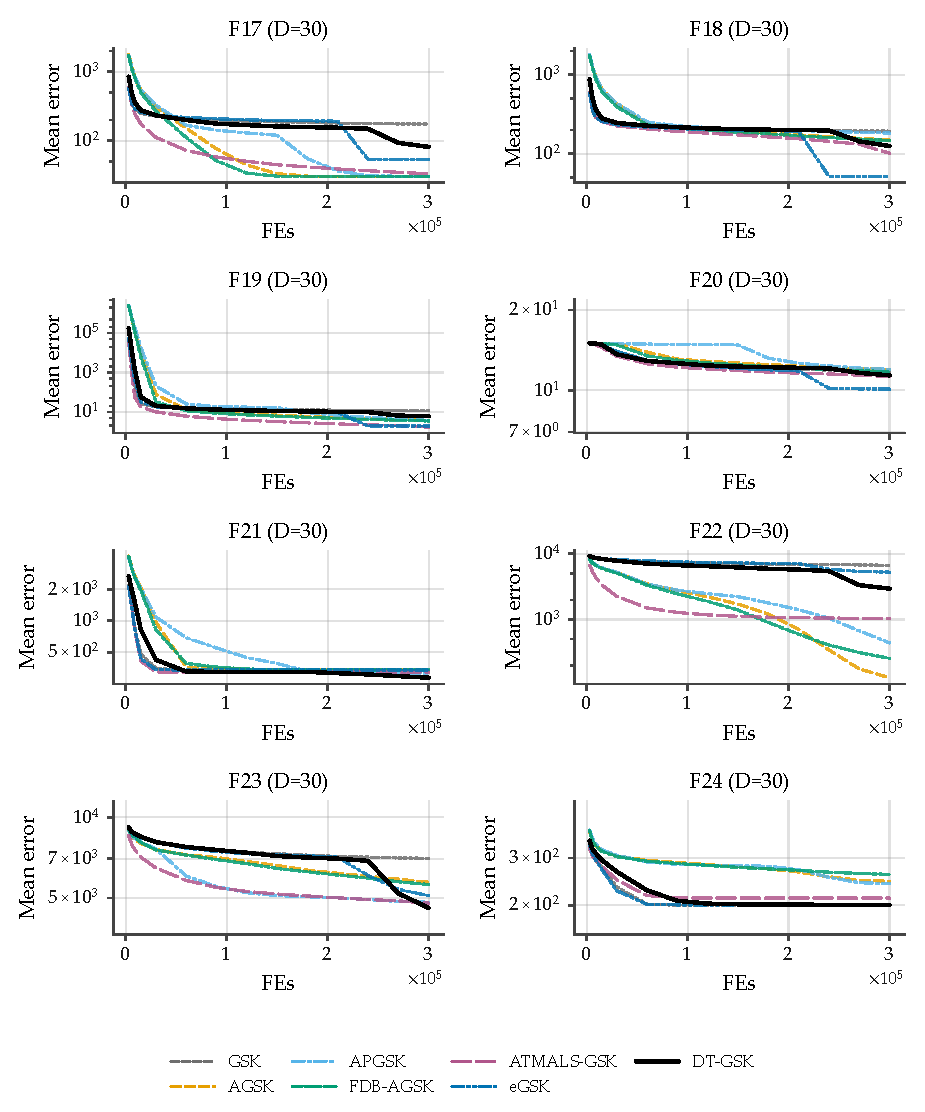
\includegraphics[width=\textwidth,height=0.87\textheight,keepaspectratio]{figures/convergence/cec2013_c}
\caption{Family-overlay convergence on the CEC2013 second comparison
suite at $D = 30$, functions F17--F24 (sub-grid c of 4): per-checkpoint
mean error across 51 runs per algorithm, 7-curve overlay, log-error
$y$-axis (display floor $10^{-14}$), one shared legend.  All panels
carry 7/7 series.  }\label{fig:sconv-cec2013-d30-c}
% BIND: FIG-CONV-CEC2013-D30-C (AN-CONV-2013-D30)
\end{figure}

\begin{figure}[H]
\centering
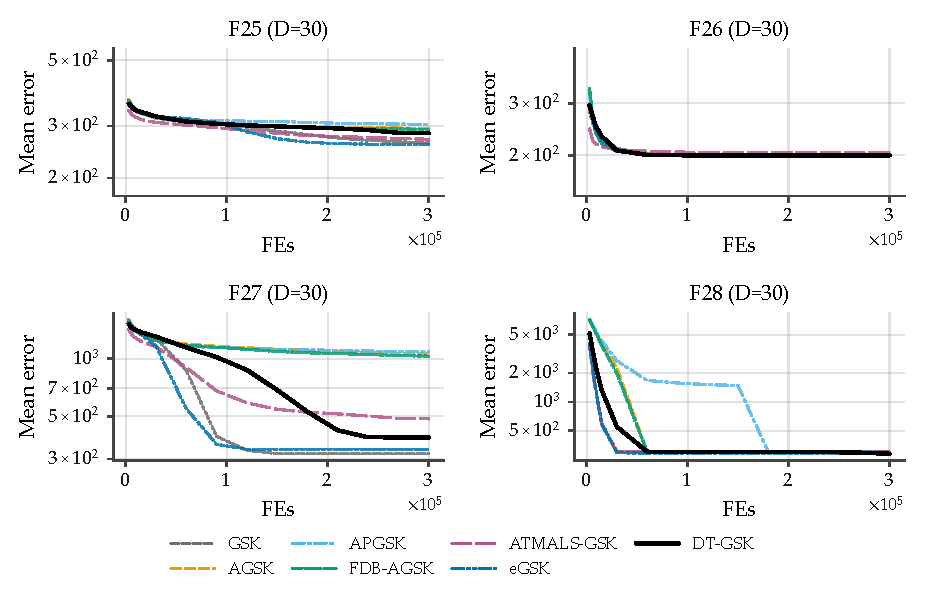
\includegraphics[width=\textwidth,height=0.87\textheight,keepaspectratio]{figures/convergence/cec2013_d}
\caption{Family-overlay convergence on the CEC2013 second comparison
suite at $D = 30$, functions F25--F28 (sub-grid d of 4): per-checkpoint
mean error across 51 runs per algorithm, 7-curve overlay, log-error
$y$-axis (display floor $10^{-14}$), one shared legend.  All panels
carry 7/7 series.  }\label{fig:sconv-cec2013-d30-d}
% BIND: FIG-CONV-CEC2013-D30-D (AN-CONV-2013-D30)
\end{figure}

%==================================================================
\section{Population-Schedule Visualization and Diagnostic Availability}\label{sec:supp:diagnostics}
%==================================================================

Figure~\ref{fig:nlpsr-schedule} plots the analytic trajectory of the
tier-floored Nonlinear Population-Size Reduction (NLPSR) schedule under
the frozen configuration for all four dimension tiers
($NP_{\text{init}} = 5D$; $N_{\min} = 12/12/25/25$ for
$D = 10/30/50/100$): population size versus consumed budget fraction.
% BIND: FIG-NLPSR (phase_03/equation_registry.csv E5; phase_03/parameter_table.md)
This is an analytic evaluation of the frozen schedule formula and
contains no empirical result values; it is included so that the
population-size trajectory quoted in the main paper can be inspected
without re-deriving the schedule.

\begin{figure}[H]
\centering
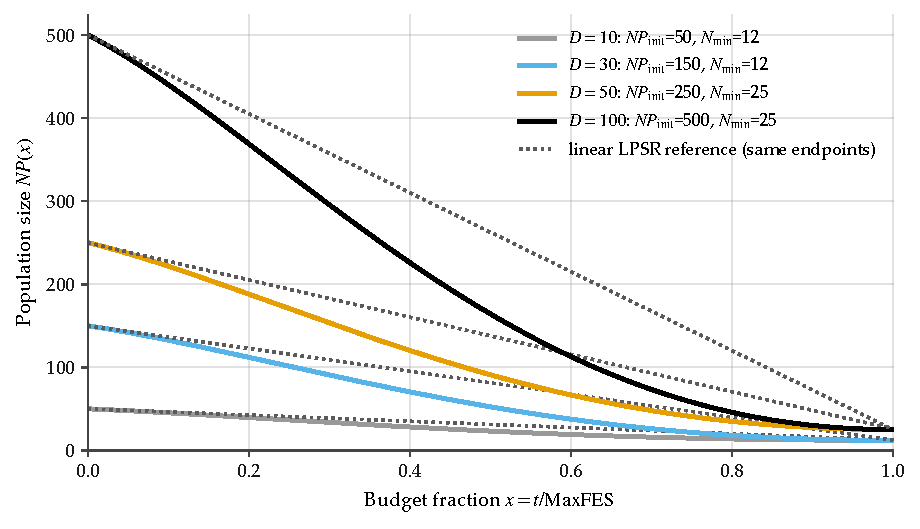
\includegraphics[width=0.85\textwidth]{figures/concept/fig_nlpsr_schedule}
\caption{Analytic trajectory of the tier-floored nonlinear population
size reduction schedule under the frozen configuration for all
four dimension tiers ($NP_{\text{init}} = 5D$;
$N_{\min} = 12/12/25/25$): population size vs.\ consumed budget
fraction.  Analytic evaluation of the frozen formula --- no empirical
result values.}\label{fig:nlpsr-schedule}
% BIND: FIG-NLPSR (phase_03/equation_registry.csv E5; phase_03/parameter_table.md)
\end{figure}

Per-generation mechanism-trace figures (interaction-structure-memory
traces and the adaptive-parameter panel) are not included in this
Supplementary Material: no promoted per-generation diagnostic release
exists in the accompanying evidence release, so these
exhibits cannot be produced under the strict-source rule of
Section~\ref{sec:repro} and are disclosed as unavailable rather than
substituted or fabricated.
% BIND: EG-005 (papers/governance/evidence_gap_register.md)

%==================================================================
\section{Reproducibility Appendix}\label{sec:repro}
%==================================================================

This appendix documents the mechanisms that make every reported number
re-derivable from the released artifacts: the paired
optimizer-independent seed schedule, the hash-frozen configuration, the
promoted read-only evidence release, and the deterministic RNG layer.
% BIND: CN-02
No byte-stability guarantee is extended to comparator
reimplementations; the guarantees below are properties of the \dtgsk{}
implementation and of the evidence pipeline.
% BIND: CN-02 (blocked-wording guard); MT-10

\subsection{Seed Schedule and Pairing}\label{sec:repro:seeds}

Every run in the evidence release is seeded by one deterministic,
optimizer-independent formula keyed on the (dimension, function, run)
triple, with base seed $20240620$:
% BIND: seed_and_pairing_audit.md Section 1 (src/gsk_family/runners/seed_policy.py get_cec_seed)
\begin{equation}\label{eq:supp-seed}
\mathrm{seed}(D, f, r) \;=\;
\bigl(20240620 + 1000003\,D + 1000033\,f + 1000037\,r\bigr)
\bmod 2147483646 \;+\; 1 .
\end{equation}
% BIND: seed_and_pairing_audit.md Section 1 (base seed 20240620; strides 1000003/1000033/1000037; modulus 2147483646)
The generator is the counter-based threefry generator in every
panel cell.
% BIND: seed_and_pairing_audit.md Section 1 (rand_generator = threefry)
Because the formula contains no optimizer term, run $r$ of any two panel
algorithms on the same (suite, function, dimension) cell consumes the
same seed and starts from the same runner-generated shared initial
population $X_{0}$; the single documented exception is \dtgsk{}
self-initialization, which draws its own $5D$-point initial population
from the same seed-paired stream.
% BIND: PR-06; seed_and_pairing_audit.md Section 4
The evidence audit recomputed every row of every stored seed
schedule against Equation~(\ref{eq:supp-seed}) --- 70{,}813 stored schedule rows
across the 21 (suite, optimizer) cells, plus the APGSK CEC2017
low-dimension seeds recovered and verified from the surviving generation
logs after their single-file sidecars were overwritten by a later run --- with zero mismatches, zero
duplicate keys and, within each schedule, zero duplicate seed values (the
schedule is intentionally optimizer-independent, so the same key maps to
the same seed across all seven algorithms --- the basis of the paired
comparison), and verified pairing validity for every comparator pair on
the primary release's three suites.
% BIND: seed_and_pairing_audit.md Sections 2 and 4 (70,813 rows; 0 mismatches; 21 cells)

Within a run, a 13-substream append-only, prefix-locked counter-based
RNG layer child-seeds all subsystems from the one run seed
($\mathrm{stream}_{k}$ for $k \in \{0, \dots, 12\}$, with stream~0 the
run seed verbatim), so toggling any subsystem cannot disturb any other
subsystem's draw order --- the property that makes exact reproduction
byte-stable and test-enforced. Table~\ref{tab:notation-rng} gives the
substream key referenced by the main-text core notation table.
% BIND: MT-10; phase_03/equation_registry.csv E12 (_dt_rng.py)

% RNG substream key (ART-NOTATION; label tab:notation-rng). N-015 relocated
% this rarely-referenced key out of the main-text notation table to the
% reproducibility section, where the substreams are specified.
\begin{table}[H]
\caption{RNG substream key. The 13 append-only, prefix-locked substreams of
the counter-based (threefry) layer, child-seeded from the single run
seed; stream~0 is the run seed verbatim (self-init).}
\label{tab:notation-rng}
\centering
\footnotesize
\begin{tabular}{@{}l@{\hspace{1.2em}}p{0.66\textwidth}@{}}
\toprule
\textbf{Symbol} & \textbf{Meaning}\\
\midrule
13 substreams & init, core, ace, kexp, div, bse, arch, link, de, control, flow, basin, trust (append-only, prefix-locked)\\
$\text{init}=\operatorname{threefry}(\text{seed})$ & stream 0 = run seed verbatim (self-init)\\
$M_{\mathrm{seed}}$ & maximum safe seed (child-seed modulus)\\
\bottomrule
\end{tabular}
\end{table}
All objective evaluations, including polish and escape evaluations, are
charged through a single strict budget-accounting path, so runs are
budget-exact, monotone, and repeat-identical per the frozen
deterministic trace.
% BIND: MT-11; algorithm_freeze_manifest.json evaluation_accounting

\subsection{Frozen Configuration and Freeze Manifest}\label{sec:repro:freeze}

Table~\ref{tab:comparator-params} lists the parameter settings of the six
comparators --- GSK~\cite{mohamed2020gaining}, \agsk{}~\cite{mohamed2020agsk},
\apgsk{}~\cite{apgsk2021}, \fdbagsk{}~\cite{fdbagsk2023},
\atmals{}~\cite{alfadli2025atmals} and \egsk{}~\cite{jawad2024egsk} --- exactly
as run here, so comparator fairness can be checked against stated values rather
than inferred from six source publications. Every entry is read programmatically
from the shipped optimizer modules; the frozen run\_config.json records
an empty optimizer\_options for each comparator, so those module
defaults are the settings of record.

\begin{table}[H]
\caption{GSK-family comparator parameter settings as run in this study. Values
are read from src/gsk\_family/optimizers/ (module constants imported;
\_option\_value and np.arange defaults extracted from source),
never hand-transcribed. Pools are written first:step:last. \dtgsk{} is
omitted here: its frozen tier-resolved configuration is given in full in the
main-text parameter table.}\label{tab:comparator-params}
% BIND: generated by papers/scripts/generate_comparator_params.py from the
% shipped optimizer modules -- read, never hand-transcribed
\centering
\tablesize{\footnotesize}
\resizebox{\textwidth}{!}{\begin{tabular}{@{}l p{11.4cm}@{}}
\toprule
\textbf{Algorithm} & \textbf{Parameter settings as run} \\
\midrule
GSK & NP = 100; Kf = 0.5; Kr = 0.9; K = 10.0; p = 0.1 \\
AGSK & NPinit = 100; NPmin = 12; Kf pool = [0.1, 1, 0.5, 1]; Kr pool = [0.2, 0.1, 0.9, 0.9]; Kw init = [0.85, 0.05, 0.05, 0.05]; p = 0.05 \\
APGSK & NPinit = 100; NPmin = 12; Kf pool = [0.1, 1, 0.5, 1]; Kf pool (neg.) = [-0.15, -0.05, -0.05, -0.15]; Kr pool = [0.2, 0.1, 0.9, 0.9]; Kw init = [0.85, 0.05, 0.05, 0.05]; p = 0.05 \\
FDB-AGSK & NPinit = 100; NPmin = 12; FDB case = 1; Kf pool = [0.1, 1, 0.5, 1]; Kr pool = [0.2, 0.1, 0.9, 0.9]; p = 0.05 \\
ATMALS-GSK & NP = 100; Kf pool = 0.2:0.1:0.8 (7 values); Kr pool = 0.85:0.01:1 (16 values); K pool = 8:1:30 (23 values); p pool = 0.05:0.01:0.15 (11 values); PLS pool = 1:0.1:2 (11 values) \\
eGSK & NP = 100; Kf1, Kf2 = 0.5; Kr = 1; K = 10; p = 0.1; late-stage frac. = 0.75; IP budget frac. = 0.002 \\
\bottomrule
\end{tabular}
}
\end{table}

The complete shipped configuration of \dtgsk{} is the single
dimension-aware configuration, tier-resolved over
$D \in \{10, 30, 50, 100\}$ and identical across the four
bound-constrained suites (no per-suite tuning), with the single
disclosed CEC2013LSGO linkage-block exception (Section~S7).
% BIND: ART-PARAMS (phase_03/parameter_table.md; algorithm_freeze_manifest.json)
The configuration and the implementing sources are hash-frozen in the
committed algorithm freeze manifest
(algorithm\_freeze\_manifest.json).  Because the method was frozen
\emph{before} a post-freeze code audit found two implementation defects, the
provenance of the shipped code is a short chain rather than a single freeze, and
we record it in full.

% BIND: M-031 provenance chronology; algorithm_freeze_manifest.json (per-file SHA-256,
%   subsystem Merkle digest) + main_manuscript_freeze_manifest.json; every printed hash,
%   anchor and date is checked against those manifests by validate_provenance_claims.py
\begin{enumerate}\itemsep2pt
\item \textbf{Original freeze (2026-07-10, anchor 708a927bf).}  The
  manifest pinned the core sources under their production filenames ---
  ism\_gsk.py a274e0f83b4efd3c,
  \_ism\_core.py 1ef815cee5d4c9c3,
  \_ism\_profiles.py c3dcdce3a3477dca,
  \_ism\_rng.py db1cc028b3ebc145 --- with a Merkle digest over
  the subsystem sources (e532fc4435fd407cf585c5ee57ba3de8).  The evidence
  produced under this freeze was release rel-2026-07-10-262fc16c9.
\item \textbf{Post-freeze audit.}  Two defects were found in the frozen core: a
  final-polish stale-incumbent fault (C006), which changes trajectories wherever
  the polish fires, and a wrong module path in the interaction graph's guarded
  numba import (M038), which silently selected the \textsc{NumPy}
  fallback and affected wall-clock only.  Both are described with their measured
  consequences in Section~\ref{sec:supp:ablation:caveats}.
\item \textbf{Source fixes and locks.}  Both defects were fixed in the source and
  each is pinned by a regression test that \emph{fails on the pre-fix code}
  (test\_dt\_polish\_incumbent\_consistent.py for C006;
  test\_dt\_graph\_backend\_parity.py for M038, which additionally
  asserts that the compiled and \textsc{NumPy} backends are bit-identical).
\item \textbf{Module rename.}  The shipped modules were renamed to
  dt\_gsk.py, \_dt\_core.py, \_dt\_profiles.py and
  \_dt\_rng.py when the method was renamed to \dtgsk{}.
\item \textbf{Full regeneration.}  The primary-panel, scaffold and overlay
  evidence was regenerated end to end with the corrected binary at 51 runs per
  cell.  Comparator cells were verified byte-identical to the prior release
  during minting, so the regeneration is scoped to \dtgsk{}.
\item \textbf{Intermediate release (anchor 78f075cb0).}  The regenerated
  evidence was first promoted as release rel-2026-07-16-78f075cb0
  (3{,}403 files), superseding rel-2026-07-10-262fc16c9.  It has since
  been superseded in turn (next item) and is retained here only as a link in the
  provenance chain.
\item \textbf{Current release (anchor 67d9345f9).}  The evidence
  accompanying this article is release rel-2026-07-20-67d9345f9 (anchor
  commit 67d9345f9502a9a584e645fa8948f60a61d70e29; 3{,}403 files), which
  supersedes rel-2026-07-16-78f075cb0.  The remint re-timed \dtgsk{} with
  the compiled interaction-graph kernels active after the M038 fix: the scientific
  columns (error, best\_fitness, seed, nfes,
  termination) are byte-identical to the prior release and only
  runtime\_seconds changed.  It also carries the regenerated
  tie-corrected Friedman statistics (M-026) and the paired rank-biserial effect
  sizes (M-027).  Every number reported in this paper and in this Supplementary
  Material is drawn from rel-2026-07-20-67d9345f9.
\end{enumerate}

\noindent The four SHA-256 prefixes recorded in the original freeze manifest are
therefore \textbf{historical}: they pin the pre-fix sources under their pre-rename
filenames and do \emph{not} match the shipped modules. A current manifest,
algorithm\_freeze\_manifest\_2026-07-19.json, was minted from the
post-fix source and records the full SHA-256 of each shipped module together
with a Merkle digest over the subsystem sources; the original is retained,
marked superseded, as the record of the 2026-07-10 freeze. The shipped modules'
current prefixes are
dt\_gsk.py 51b12194a3962a20,
\_dt\_core.py 3ce5db5291dcda4d,
\_dt\_profiles.py 7baadf228d356394 and
\_dt\_rng.py 8a0fc27d7531b847.
What the manifest continues to guarantee is that the shipped configuration is
immutable and machine-checked: the repository's configuration-lock validator and
the byte-stability regression test enforce byte-identity of the \emph{current}
sources on every run, so the code that produced the current release cannot drift
without failing the gate.


\noindent One source file has changed since the evidence release was promoted.
\_dt\_core.py was modified after \mbox{rel-2026-07-20-67d9345f9} by a
performance campaign (change requests CR-0013 to CR-0018) that removed redundant
memory traffic, dead computation and dead code from the per-generation loop; its
prefix above is the post-campaign value, and the release was produced by
dc2d59db91a288ee. Every one of those edits was certified
\emph{bit-identical}: the campaign introduced a pinned end-to-end regression
matrix (seven optimizers across six benchmark suites, exact hexadecimal
\mbox{best-fitness} values) and re-verified all eighty-four cells of a
cross-suite measurement ledger against their pre-campaign values, with zero
divergence, alongside the generator known-answer tests and the byte-stability
pins. One exception is recorded rather than left to be found. The internal
control of Table~\ref{tab:rev-e3} re-executes, under the current revision,
runs archived under the earlier one; it does not reproduce them exactly, and
its win/tie/loss count carries that residual. The residual's origin has since
been demonstrated by a promoted re-execution (release g1-rel-2026-08-28-65b3d39e6):
re-running the five carrier functions at $D = 100$ under the current build,
with the numeric stack pinned to one thread, reproduces the transplant arm on
all 26 divergent cells and the archived values on none, while reproducing
both on all 229 agreeing cells, with zero seed mismatches --- a difference
between builds, not a within-build instability, and that table's caption now
reports it as such. No other reported number, rank, $p$-value or decision
in this paper or this Supplementary Material depends on which of the two
revisions is used, and the archived release from which every reported number
is derived is itself unchanged.
% BIND: algorithm_freeze_manifest.json frozen_core_sources (historical); shipped-module hashes at the current anchor
Any post-freeze change to the frozen sources, the configuration, or the
mechanism inventory requires a recorded change request; the two corrections
above are registered as CR-0007 in
papers/governance/change\_request\_register.csv, together with the
regeneration scope they forced.
% BIND: algorithm_freeze_manifest.json change_control; change_request_register.csv CR-0007; M-031

\subsection{Configuration Selection and Development Protocol}\label{sec:repro:tuning}

The single dimension-aware configuration is fixed once and reused across
all five suites, with the single disclosed CEC2013LSGO linkage-block
exception (Section~S7); this subsection discloses \emph{how} it was selected, so the
primary-suite comparison can be read with its selection exposure in view.
% BIND: R6-T03 (development-suite / selection-exposure disclosure)
CEC2017 was the \emph{development suite}: the tier-resolved parameter values
were set against CEC2017 at the reported budget and run count ($n=51$), and no
CEC2011 or CEC2013 result was consulted during configuration selection --- those
two suites are held out with respect to the tuning choices. No CEC2020 or
CEC2013LSGO result existed when the configuration was frozen; the sole
later configuration change --- the two CEC2013LSGO linkage-block-size
entries --- is disclosed with its timing in Section~S7. Before the final
configuration was promoted, \textbf{six} full-panel candidate configurations ---
including the one ultimately selected --- were
compared against the complete seven-algorithm family panel on CEC2017. ``Full
panel'' is the criterion that defines this count: each candidate was run against
all seven algorithms on the full function set, not through a smoke test, a
function or dimension subset, or an isolated component experiment. The count
therefore \emph{excludes} preliminary debugging and smoke runs,
partial-function or partial-dimension pilots, single-component ablations and
sensitivity checks, failed or incomplete configurations, and all post-selection
validation, correction, and evidence-regeneration runs. This selection exposure
is disclosed as an author-attested development-history note: the
intermediate candidates predate the immutable evidence release and are not part
of it, so the figure rests on the authors' record rather than on a released
artifact, and it is stated rather than absorbed silently. Consequently the CEC2017 headline (best overall Friedman mean rank)
is a result \emph{on the development suite} and should be read as such: the
suites that did not inform selection place \dtgsk{} second on CEC2011 (a
Holm-significant loss to \egsk{}), third on CEC2013 at $D = 30$ but first
overall (2.80), fourth on the pre-registered CEC2020, and tied-first
descriptive on CEC2013LSGO; the non-development evidence is therefore
mixed --- strongest where the tiered subsystems are active and weakest
where they are structurally off --- rather than uniformly favorable or
unfavorable. This tempers ---
without eliminating --- the optimistic-selection concern and bounds how far the
primary-suite standing should be generalized.

\subsection{Limitations in Full}\label{sec:repro:limitations}

The conclusions summarize the limitations that bound this study; they are
stated here in full, with the numeric evidence for each. The wording
follows the conclusions of the submitted manuscript, so that nothing is
softened in transit.
% BIND: N-020 (limitations carried from the conclusions; synchronized with the CR-0019 revisions)

\paragraph{Limitations.}
Several limitations bound these findings. First, the mid-dimension tier
favors \egsk{}. At CEC2017 $D = 30$, \dtgsk{} is second (2.50
vs.\ 2.29) with an 11--2--16 head-to-head record; on CEC2013 at
$D = 30$ it is third, and \egsk{} also leads CEC2011. The rank deficit
is real. It is not statistically separable at this dimension
($p_{\mathrm{Holm}} = 0.199$), which bounds how strongly either standing
should be read, in both directions. % BIND: LM-01 (AN-OMNI-2017-D30; AN-PW-2017-D30; AN-OMNI-2013-D30; AN-OMNI-2011-NATIVE)
Second, the structure memory and the polish are gated to $D \geq 50$
under the frozen configuration, so at $D \leq 30$ \dtgsk{} runs essentially
the adaptive scaffold: low-dimension behavior reflects this structural
gating rather than the tier-gated mechanisms, the memory itself depends
on accepted moves --- a stalled run feeds it no signal --- and the
polish fires at most once, with whatever basis has been
learned. % BIND: LM-02 (gating as design fact; mechanism failure modes)
Third, every comparative finding is panel-relative by design: the study
establishes standings within the seven-algorithm GSK family on the five
suites at the stated budgets. The cost is external calibration --- no
claim is made relative to other metaheuristic families or to CEC
competition winners, and none can be read from these results. What the
scope does buy is attribution: one code base, one protocol and one
harness, so within-panel deltas reflect algorithmic differences up to the
port and initialization asymmetries disclosed below. % BIND: LM-03
Fourth, the \egsk{} panel cells derive from a port whose SLSQP polish
substitutes the reference implementation's fmincon-based solver. Cross-implementation
runtime and environment comparability is therefore limited, and no
runtime-superiority claim is made anywhere in this paper. The main-text runtime table reports
\dtgsk{}'s own per-run cost only --- comparator timings came from a separate
measurement session, so no cross-algorithm runtime comparison is drawn. These costs were
measured with the interaction graph's compiled kernels active: an
earlier release had silently executed the bit-for-bit-equivalent
\textsc{NumPy} reference path, inflating wall-clock only, and the
affected timings were re-measured in the 51-run regeneration
(Supplementary Material, Section~S6.7). % BIND: LM-04 (comparability_audit.md; AN-COST-2017); backend fixed + re-measured in the 2026-07-16 campaign
Fifth, each suite's evidence stops at its own tested dimensions:
$D \le 100$ on CEC2017, $D \le 50$ on CEC2013, native dimensions on CEC2011,
$D \le 20$ on CEC2020, and $D = 1000$ (family-internal, post-hoc, 25 runs
per cell) on CEC2013LSGO. The component-isolation evidence stops at
$D \le 100$: no component contrast was run at the CEC2013LSGO scale, so
the large-scale standing attributes nothing to the memory or the polish
in either direction. At $D = 1000$ no member of the family, \dtgsk{}
included, approaches the performance that dedicated large-scale
specialists report in the literature; the family's evidence of
competitiveness therefore ends at the dimensionalities of the
bound-constrained suites. % BIND: LM-05 (revised, CR-0019: per-suite ceilings; component-isolation ceiling D<=100; no component attribution at D=1000); LM-06
Sixth, the study runs on a single host and environment: no
independently verified second-environment cell exists, the run-time
NumPy/SciPy versions behind \egsk{}'s SciPy-SLSQP polish are not
captured in the evidence release (only the analysis bundle's own
environment is), and byte-identical reproduction at $D \geq 50$ requires
single-threaded numerical kernels, which caps parallel speed-up at the
high-$D$ tiers where \dtgsk{}'s per-run cost is largest.
% BIND: comparability_audit.md (single-host row: no second-environment cell); fp_environment_audit.md E2 (run-time numpy/scipy uncaptured); implementation_correspondence.md note 2 (single-thread precondition)
Seventh, the comparison is entirely within the GSK family. As
disclosed in the Conflicts of Interest, five of its six comparators were
authored or co-authored by two of the present authors. No external, non-GSK
baseline --- an L-SHADE-class or CMA-ES method, or a structure-learning
method such as differential grouping --- is evaluated to calibrate the
family against the broader state of the art, so the standings are
interpretable only within this panel and not as a placement in the
wider field. Relatedly, \dtgsk{}'s self-initialization (the documented
shared-$X_{0}$ exception) means that no \dtgsk{} cell begins from the
shared initial population --- the self-init applies at every dimension
--- a disclosed fairness asymmetry that is not separately bounded and is
most consequential at low dimension, where \dtgsk{} runs essentially the
scaffold.
% BIND: LM-03 (within-family panel scope); comparability_audit.md; main.tex conflictsofinterest; PR-06 (self-init exception)
Eighth, three attribution gaps bound what the component evidence can say.
The corroborative weight rests on the two suites held out from
configuration selection, CEC2011 and CEC2013: CEC2017 is
\emph{development-exposed} --- it
informed the frozen configuration and is also the source of the headline
rank --- so its standing is a performance estimate on a tuned-against
suite rather than an untouched confirmatory one. The
final-polish isolation removes the \emph{entire} deterministic compass
endgame, so any effect it measures attaches to that phase as a whole, not to the
\emph{learned} eigenbasis it consumes.  That question is now answered for the
coordinate comparison: Section~\ref{sec:supp:rev:basis} isolates the three arms
directly and finds the plain coordinate axes \emph{outperform} the learned
eigenframe at $D = 50$.  A matched random orthonormal basis was not tested and
remains open. And the evidence-bearing runs carry no
component-level evaluation ledger or memory-activation trace, so we cannot
report how many evaluations each modifier consumed, nor how often the
learned structure was actually exposed to its consumers; the standalone
null is therefore ``no detectable benefit under this design'' and not a
demonstration that the memory was active and neutral.
% BIND: development-exposure disclosure; basis-isolation gap (M036); component-FES/activation ledger absent (M031, M052)
Ninth, the parameter-sensitivity evidence is exploratory and narrow.  The
sweep of Section~\ref{sec:supp:rev:sensitivity} covers seven constants at two
levels, at $D = 30$ and $D = 100$ only, with 15 repetitions per cell against the
frozen panel's 51, and it leaves the dimension-tier boundaries
themselves unvaried, so their sensitivity is untested.  Neither ARGP nor the deep-stall
restart is isolated by the remove-one study, which excludes both by
pre-specification (Section~S6.2).

Beyond these, the statistical scope is itself bounded: inference rests
on 29-function and 22-problem blocks under rank-based tests; run-level
records against \apgsk{} on CEC2017 at $D \leq 50$ were unavailable at
analysis freeze (recovered post-freeze), leaving
function-level tests as the frozen basis there; and the single frozen
configuration was applied with no
per-suite tuning, whose protocol disclosure is in the Supplementary
Materials. % BIND: negative_findings.md item 8 (APGSK gap); ART-PARAMS

\subsection{Sensitivity of the Win/Tie/Loss Tally to the Tie Band}\label{sec:repro:tieband}

The reported win/tie/loss counts use a fixed absolute tie band,
$|\Delta| < 10^{-8}$, applied uniformly to every function. That band is
deliberately conservative, but it is not scale-free: on functions whose error
scale is of order $10^{3}$ it admits no ties at all, while on functions solved to
the reporting floor it absorbs every difference. It is therefore worth asking
whether the tally is an artifact of that choice.

Recomputing the CEC2017 counts from the same frozen per-function means under a
\emph{relative} band --- a tie when
$|a-b| \le \rho \max(|a|,|b|)$, retaining the $10^{-8}$ floor --- leaves the
direction of every panel cell unchanged at $\rho = 1\%$ except one, and changes
two cells at $\rho = 5\%$. Both are \egsk{} cells at the upper tiers: at
$D = 50$ the 13--0--16 record becomes 12--7--10, and at $D = 100$ the 12--0--17
record becomes 12--5--12. No other comparator changes direction at either
threshold.

This is consistent with, rather than contrary to, the result reported in the main
text. Those are precisely the two cells whose Holm-corrected tests are \emph{not}
significant ($p_{\mathrm{Holm}} = 1.0$ and $0.795$), and where the paper already
states that \dtgsk{} and \egsk{} are not separable. The sensitivity shows that
the apparent margin in those cells depends on how a tie is defined, which is an
argument for reading them as ties in both directions --- not as evidence for
\dtgsk{}. Every Holm decision, every Friedman rank, and every reported
significance is computed from the tests themselves and is unaffected by the tie
band, which enters only the descriptive counts.
% BIND: N-005 (recomputed from descriptive_stats_cec2017_D*.csv; no optimizer runs)

\subsection{Legacy Identifiers}\label{sec:repro:aliases}

The method and its structure-memory subsystem were renamed during development,
and the released artifacts retain the earlier identifiers wherever a hash or a
directory name would otherwise change. Table~\ref{tab:aliases} maps each current
name to the legacy one, so a reader working directly with the evidence release
can resolve a name that no longer appears in this paper. Only the identifiers
changed; no algorithm, configuration value, or result is affected.
% BIND: N-008 (alias map for legacy identifiers)

\begin{table}[H]
\caption{Current names and the legacy identifiers retained in released
artifacts.}
\label{tab:aliases}
\centering
\small
\begin{tabular}{lllp{4.4cm}}
\toprule
\textbf{Current} & \textbf{Legacy} & \textbf{Scope} & \textbf{Where the legacy form persists}\\
\midrule
ISM & SGSM & subsystem name & overlay-study cell IDs; some analysis column names\\
no\_sgsm & --- & ablation cell ID & the ISM-off cell in the overlay
study; its ID embeds the legacy sgsm subsystem name, so it has no
separate legacy form\\
\_dt\_core.py & \_ism\_core.py & source file & hashes recorded in the
algorithm freeze manifest\\
\bottomrule
\end{tabular}
\end{table}

\subsection{Acronyms}\label{sec:repro:acronyms}

The main-text notation table defines every mathematical symbol. This list covers
the acronyms that appear in prose but carry no symbol, so a reader meeting one
out of order does not have to search for its first use.
% BIND: E-005 (acronyms absent from the main-text notation table)

\begin{table}[H]
\caption{Acronyms used in the text that are not mathematical symbols.}
\label{tab:acronyms}
\centering
\small
\begin{tabular}{ll}
\toprule
\textbf{Acronym} & \textbf{Expansion}\\
\midrule
ACE & Adaptive Configuration Engine (operator-configuration selector)\\
ARGP & Acceptance-Rate Gated Pruning\\
BSE & Budget-Safe Escape\\
CD & Critical Difference (Nemenyi post-hoc)\\
CMA-ES & Covariance Matrix Adaptation Evolution Strategy\\
DE & Differential Evolution\\
EWMA & Exponentially Weighted Moving Average\\
GSK & Gaining--Sharing Knowledge (the base algorithm)\\
ISM & Interaction-Structure Memory\\
JADE & Adaptive DE with optional external archive\\
MaxFES & Maximum number of function evaluations (the budget)\\
NLPSR & Nonlinear Population-Size Reduction\\
SHADE & Success-History based Adaptive DE\\
SLSQP & Sequential Least-Squares Programming (SciPy routine)\\
W/T/L & Win/Tie/Loss (tie: $|\Delta| < 10^{-8}$)\\
\bottomrule
\end{tabular}
\end{table}

\subsection{Frozen Parameters: Per-Subsystem Detail}\label{sec:repro:params-detail}

Table~\ref{tab:parameters-detail} completes the main-text
frozen-parameter table. The main text carries the run-level settings, the
core GSK operator and the population schedule; the per-subsystem constants are
collected here, where they can be set at full size rather than compressed to fit
a text block. Both halves derive from the same hash-frozen configuration and no
value is omitted.
% BIND: phase_03/parameter_table.md (canonical source); algorithm_freeze_manifest.json; N-013
% ============================================================================
% DT-GSK frozen parameter table -- PER-SUBSYSTEM DETAIL (supplement).
% Split out of parameter_table.tex under ticket N-013: the combined 48-row
% table had to be scaled to 5.3 pt to fit the main-text block, below the
% journal's 8 pt table guidance. Canonical source is unchanged:
% papers/build_prompt_phases/phase_03/parameter_table.md
% Label: tab:parameters-detail.
% ============================================================================
\begin{table}[H]
\caption{Frozen run parameters of the shipped configuration (per-subsystem
detail). Companion to the main-text frozen-parameter table, which carries the
run-level and core-operator settings. Where a value varies by dimension tier the
four tiers $D{<}20$ / $20$--$49$ / $50$--$99$ / ${\ge}100$ are shown. No tuning
is required or permitted at run time; hash-frozen in
algorithm\_freeze\_manifest.json.}
\label{tab:parameters-detail}
\centering
\small
% All three columns are wrapping p{} columns. As bare `l' columns the longest
% Value/Parameter/Notes rows ran up to 219 pt past the portrait text block and
% clipped at the page edge (panel review, 2026-07-23); a first pass wrapped only
% Notes and still left a 147 pt overrun from the wide Parameter/Value rows
% (e.g. the D>=100 controller list). Fixed widths (3.0+5.4+4.8 cm plus column
% separation) keep every row inside the ~15.7 cm portrait text block.
\begin{tabular}{p{2.9cm} p{5.8cm} p{4.8cm}}
\toprule
\textbf{Parameter} & \textbf{Value} & \textbf{Notes}\\
\midrule
\multicolumn{3}{l}{\emph{ACE / ARGP}}\\
\midrule
arm pool & 5 arms $(KF,KR,K_{\exp})$; arm 3 = GSK-pure $(0.5,0.9,10)$; at $20{\le}D{<}100$ a virtual sixth DE/rand/1 arm is appended, so the pool holds 5 / 6 / 6 / 5 arms across the four tiers & the sixth arm is added at run time (see the DE-arm row)\\
init probs $\pi_0$ & $(0.05,0.05,0.45,0.05,0.40)$ at $D{<}20$ and $D{\ge}100$; with the DE arm ($20{\le}D{<}100$) the five are rescaled by $1-\pi_{\mathrm{DE}}$ and a sixth appended, giving $(0.05,0.05,0.40,0.05,0.355,0.095)$ at $20$--$49$ and $(0.05,0.05,0.35,0.05,0.31,0.19)$ at $50$--$99$ & shown after the $\pi_{\min}$ simplex projection\\
learning rate $c$ & 0.10 & \\
probability floor $\pi_{\min}$ & 0.05 & \\
memory mode & single ($D{<}20$) $\to$ top\_bottom ($D\ge20$) & \\
DE arm & off ($D{<}20$, $D\ge100$) / on ($20{\le}D{<}100$) & \\
ARGP window / threshold & 30 / 0.02 (0.010 at $D\ge50$), warmup 0.15 & \\
\midrule
\multicolumn{3}{l}{\emph{Linkage crossover}}\\
\midrule
minimum dimension & 10 ($D{<}50$) / 30 ($D\ge50$) & the blockwise mask is off entirely below it\\
block size & 5 ($D{<}50$) / 10 ($D\ge50$) & \\
mix probability & 0.70 ($D{<}20$) / 0.40 (mid) / 0.70 ($D\ge50$) & \\
refresh period & 20 gen.\ ($D{<}50$) / 10 ($D\ge50$) & \\
\midrule
\multicolumn{3}{l}{\emph{BSE / archive / deep-stall}}\\
\midrule
trigger mode & stagnation ($D{<}20$) / triple ($D\ge20$) & \\
window $W$ & 50; signal window 10 & \\
$\epsilon$ & $10^{-8}$ & \\
restart fraction $r_{\text{rst}}$ & $0.30$ ($D{<}50$) / $0.10$ ($D\ge50$) & \\
max restarts $R_{\max}$ & 4 ($D{<}20$, $50{\le}D{<}100$) / 2 (otherwise) & \\
acceptance / diversity floor & 0.10 / 0.35 & \\
archive size / distance & fixed cap 200 (all $D$), L2 0.05 & $1.5\,NP_{\text{init}}$ fallback inert (cap set)\\
deep-stall & on; frac 0.25; min-budget 20\,000; & cooldown 0.15; stop 0.9\\
\midrule
\multicolumn{3}{l}{\emph{ISM / eigenframe polish ($D\ge50$)}}\\
\midrule
enabled & $D\ge50$ & interaction\_graph\_min\_dim=50\\
decay $\lambda$ & 0.95 & interaction\_graph\_decay\\
learning rate $\eta$ & 1.0 & interaction\_graph\_lr\\
refresh period / warmup & 5 gen.\ ($D{<}100$) / 20 ($D\ge100$); warmup 0.10 & \\
confidence gate $\kappa_{\min}$ & 0.35 (linkage 0.35, LS 0.45) & adaptive at $D\ge50$: window 30, percentile 0.50, floor 0.12\\
block size range & 2--10 & \\
final polish start & $0.96$ & final\_polish\_start\_frac\\
restart response & matrix decay 0.50 (interaction\_restart\_decay); post-escape cooldown 5 gen.\ & applied on each BSE escape event (not on the deep-stall restart)\\
\midrule
\multicolumn{3}{l}{\emph{$D\ge100$ controllers}}\\
\midrule
A1 late-accept clip & $\tau$-floor 0.85; high-acc 0.30; log-drop $\epsilon$ $-2.0$; streak $k{=}5$; strict $\epsilon$ $10^{-3}$; log-drop EMA $\alpha$ 0.30 & tightens elitist acceptance late in budget\\
A2 frozen-streak broaden & acc-floor 0.05; log-drop $\epsilon$ $-3.0$; streak $k{=}10$; window/cooldown 20/10 gen.; $KR$ factor 1.5 & broadens $KR$ during frozen streaks\\
FC4 late linkage random-mix & $\tau$-floor 0.50; negative-lift $-0.05$; severe-lift $-0.20$; strength 0.5; lift-EMA $\alpha$ 0.20 & reverts to random linkage when learned-block lift turns negative\\
basin memory / subspace-sampling floor & enabled & \\
budget/ROI gate & admits the coordinate local search only from consumed budget fraction $0.70$ & duplicates this tier's local-search start fraction, but is read before the escape rather than after it; the trust-region displacement governor it descends from was removed from the code at the paper freeze\\
\bottomrule
\end{tabular}
\end{table}


\subsection{Complete Operator Specification}\label{sec:repro:opspec}

This subsection records the operator-level constants and update rules that the
main-text equation registry (Equations~(7), (10), (11), (12), and~(13)) summarizes, so
that \dtgsk{} is reproducible from the text.  Every value is transcribed from
the hash-frozen sources of Section~\ref{sec:repro:freeze} and is stated per
dimension tier wherever the single dimension-aware configuration resolves it
differently; the tier boundaries are $D<20$, $20\le D<50$ and $D\ge 50$ (with a
further $D\ge 100$ extension), as in the main-text dimension-gating figure.
% BIND: ART-PARAMS (_dt_core.py / _dt_profiles.py / interaction_graph.py / _dt_rng.py, hash-frozen)

\paragraph{Knowledge-construction arms of ACE (main-text Equation~(7)).}
The adaptive credit-based selector samples one of five fixed arms, each a triple
$(K_F, K_R, K_{\exp})$ of the gaining--sharing rate, crossover rate and
junior-dimension exponent, with the initial selection probabilities $\pi_0$:
\begin{center}
\small
\begin{tabular}{cccccc}
\toprule
arm & $K_F$ & $K_R$ & $K_{\exp}$ & configuration & $\pi_0$\\
\midrule
1 & 0.1 & 0.2 & 2.0  & cautious explorer            & 0.05\\
2 & 1.0 & 0.1 & 15.0 & dimension-selective bold     & 0.05\\
3 & 0.5 & 0.9 & 10.0 & GSK-canonical (baseline)     & 0.45\\
4 & 1.0 & 0.9 & 5.0  & aggressive wide              & 0.05\\
5 & 0.5 & 0.9 & 3.0  & extended-exploration GSK     & 0.40\\
\bottomrule
\end{tabular}
\end{center}
% BIND: _dt_core.py:202-209 (ace_pool arms; ace_init_probs)
The credit is an exponential moving average at learning rate $c=0.10$, the
probabilities are projected onto the simplex under the floor $\pi_{\min}=0.05$,
and updating begins once the consumed-budget fraction reaches $0.05$; the arm
memory is a single pool for $D<20$ and a top/bottom split for $D\ge 20$.  For
$20\le D<100$ an optional sixth differential-evolution arm ($F=0.5$, $CR=0.9$)
is configured at $0.10$ ($20$--$49$) or $0.20$ ($50$--$99$).  The five arm
probabilities tabulated above are the DE-off vector: when the sixth arm enters,
the five are rescaled by $1-\pi_{\mathrm{DE}}$ and the six are re-projected onto
the simplex under $\pi_{\min}$, giving $(0.05,0.05,0.40,0.05,0.355,0.095)$ at
$20$--$49$ and $(0.05,0.05,0.35,0.05,0.31,0.19)$ at $50$--$99$.  When a generation yields no net
improvement (its summed $f_{\mathrm{old}}-f_{\mathrm{new}}$ is strictly negative) the
credit target is restricted to the improving arms, as in main-text
Equation~(7); when the generation is net-improving the full-pool target is
used with worsened arms floored at $\pi_{\min}$.  The restricted branch
stabilizes learning on hard functions.
% BIND: _ace_update_probs _dt_core.py:1193-1258; ace_learning_rate/ace_start_frac/ace_min_prob _dt_core.py:210-212

\paragraph{ACE/ARGP operating cycle (per generation).}
The following states the order of operations, the timing conditions, and the
edge cases of the selector and its pruning gate. Each step names the frozen
source that implements it, so the specification can be checked line by line.

% BIND: ART-PARAMS; _ace_update_probs _dt_core.py:1193-1258;
%   ace_learning_rate / ace_start_frac / ace_min_prob _dt_core.py:210-212 (hash-frozen)
\begin{enumerate}\itemsep2pt
\item \textbf{Eligibility to update.} No credit update is applied until the
  consumed-budget fraction reaches $0.05$; before that the probabilities remain
  at $\pi_0$. \hfill ace\_start\_frac, \_dt\_core.py
\item \textbf{Arm assignment.} Each individual independently draws one arm from
  the current probability vector $\pi$ on the ACE substream; at $D\ge 20$ the
  draw uses the top/bottom memory that the individual's fitness rank selects,
  and a single shared memory below that.
  \hfill\_dt\_core.py (ACE sampling), \_dt\_rng.py
\item \textbf{Optional differential-evolution arm.} For $20\le D<100$ a sixth
  arm ($F=0.5$, $CR=0.9$) joins the pool with tier-dependent initial
  probability; it is excluded at $D<20$ and $D\ge 100$.
  \hfill ace\_de\_entry, \_dt\_profiles.py
\item \textbf{Credit accumulation.} Every individual contributes its signed
  fitness delta to the arm that drew it, giving the per-arm aggregate $d_m$ of
  main-text Equation~(7). Credit is an improvement magnitude, not an acceptance
  count. \hfill\_ace\_update\_probs, \_dt\_core.py
\item \textbf{Target selection (two branches).} With $S=\sum_m d_m$: if $S>0$
  the target is the full-pool share $d/S$; if $S<0$ and at least one arm
  improved, the target is restricted to the improving arms. If $S=0$, if $S$ is
  non-finite, or if no arm improved, no target is formed and $\pi$ is carried
  forward unchanged apart from its projection.
  \hfill\_ace\_update\_probs, \_dt\_core.py
\item \textbf{Mixing and projection.} The target is projected, mixed into $\pi$
  by an exponential moving average at rate $c=0.10$, and the result projected
  again. The projection is the Euclidean projection onto
  $\{\pi_m\ge\pi_{\min}=0.05,\ \sum_m \pi_m = 1\}$ --- not a floor followed by
  renormalization. \hfill\_ace\_project\_probs, \_dt\_core.py
\item \textbf{ARGP freeze.} After a warm-up fraction of the budget, an unfrozen
  arm whose rolling acceptance over the trailing window falls below the tier
  threshold is frozen and its mass redistributed. Freezing stops while only
  min\_active arms remain unfrozen, so the pool can never collapse to a
  single arm. In the frozen configuration the freeze test, the recovery test
  and the mass redistribution act on the pooled acceptance record and the
  mixed probability vector, and the redistributed vector is written back over
  both halves of the top/bottom memory, so that memory is reset whenever any
  arm is frozen; a per-half scope is implemented but not enabled.
  \hfill ARGP retirement branch, \_dt\_core.py
\item \textbf{ARGP unfreeze (recoverable).} A frozen arm that is sampled again
  and whose rolling acceptance recovers to the threshold is unfrozen. Pruning is
  therefore soft and reversible; no arm is permanently removed.
  \hfill ARGP retirement branch, \_dt\_core.py
\end{enumerate}

\noindent The selector consumes no objective evaluations of its own: credit is
read from evaluations the generation has already spent.
% BIND: M-008 (ACE/ARGP operating cycle); _ace_update_probs _dt_core.py:1203;
% _ace_project_probs :694; _argp_update_memory_probs :1271; _dt_profiles.py (tier constants)

\paragraph{Interaction-graph update (refinement of main-text Equation~(11)).}
The interaction-structure memory maintains an unsigned magnitude graph
$G_{\mathrm{abs}}$ and a signed graph $G_{\mathrm{signed}}$ (with an auxiliary
per-dimension self-weight and co-occurrence support used only for the confidence
of Equation~\eqref{eq:opspec-conf}).  For each accepted move $i$ with strictly
positive improvement $\delta_i$, its displacement $\Delta x_i$ (restricted to
its non-zero support) is $\ell_1$-normalized,
\begin{equation}
v^{\mathrm{abs}}_i = \frac{\lvert \Delta x_i\rvert}{\lVert \Delta x_i\rVert_1},
\qquad
v^{\mathrm{sig}}_i = \frac{\Delta x_i}{\lVert \Delta x_i\rVert_1},
\end{equation}
and the accumulators receive an improvement-weighted rank-one scatter of weight
$w_i=\delta_i\,\varsigma_i$,
\begin{equation}
G_{\mathrm{abs}} \leftarrow \lambda\,G_{\mathrm{abs}}
 + \eta\sum_i w_i\, v^{\mathrm{abs}}_i {v^{\mathrm{abs}}_i}^{\!\top},
\qquad
G_{\mathrm{signed}} \leftarrow \lambda\,G_{\mathrm{signed}}
 + \eta\sum_i w_i\, v^{\mathrm{sig}}_i {v^{\mathrm{sig}}_i}^{\!\top},
\end{equation}
after which each graph is symmetrized and its diagonal zeroed (the self-weight
is tracked separately).  The per-source weight $\varsigma_i$ is $0$ for
differential-evolution-arm moves, $0.25$ for local-search moves and $1$
otherwise; the decay is $\lambda=0.95$ and the commit rate is $\eta=1.0$ (the
$\lambda,\eta$ of main-text Equation~(11)).  Updates begin after budget fraction $0.10$
and, at $D\ge 100$, are thinned to every tenth generation and capped at the $24$
largest-improvement samples.  Because the multiplicative decay $\lambda$ is applied
every generation while evidence is injected only every tenth at this tier, the
effective decay between injections is $\lambda^{10}\approx 0.60$ rather than $0.95$;
correspondingly the per-update cost of $O(24\,D^2)$ is incurred once per ten
generations, i.e.\ an amortized $\approx O(2.4\,D^2)$ per generation, against the
$O(NP\,D^2)$ per-\emph{update} worst case at $D=50$--$99$, where every accepted move
contributes an uncapped rank-one scatter each generation.
\emph{Event-driven updates.} Two graph updates fall outside this steady cadence. First, whenever the charged coordinate local search improves at least one individual, that generation's accepted local-search displacements are injected a second time --- at the local-search source weight $0.25$ but \emph{without} the usual $\lambda=0.95$ fade (an injection at decay $1$) --- and the linkage blocks are re-extracted immediately rather than waiting for the next five-generation refresh. Second, after a budget-safe-escape event --- a partial restart, or any Cauchy perturbation, including a successful rescue that cancels the restart --- the retained graph is halved ($\times 0.50$) and a five-generation cooldown suppresses block re-use until the post-escape population has produced fresh evidence, after which blocks are re-extracted; the deep-stall restart itself does not touch the graph. Both transitions are frozen defaults of the shipped configuration.
% BIND: ig_update_from_accepted interaction_graph.py:222-368; decay 0.95 / lr 1.0 _dt_profiles.py:120-121; de/ls update weights _dt_profiles.py:141-142

\paragraph{Graph-to-block extraction and readiness.}
At each linkage refresh the magnitude graph is max-normalized,
$W = G_{\mathrm{abs}}/\max G_{\mathrm{abs}}$.  A row-wise adjacency keeps, for
each dimension $j$, the edges $W_{jk}\ge \max\!\left(\varphi,\ \tfrac12\max_k
W_{jk}\right)$ with floor $\varphi=10^{-4}$ and at most $b_{\max}-1$ neighbors
(a row with no edge above the floor retains its strongest positive edges, at
most $b_{\max}-1$, as a fallback);
it is symmetrized and its connected components are taken.  Components smaller
than $b_{\min}=2$ are discarded, those with at most $b_{\max}=10$ members are
kept whole, and larger components are split greedily (highest row-sum seed plus
its strongest neighbors).  A block feeds the linkage crossover only when the
graph is \emph{ready}: at least $10$ updates and $2$ refreshes have accrued, at
least $4$ dimensions are non-trivial, and the overall confidence
\begin{equation}\label{eq:opspec-conf}
\kappa(G) = \left(\frac{\sum_b \lvert b\rvert\,c_b}{\sum_b \lvert b\rvert}\right)
\sqrt{\mathrm{cov}},
\qquad
c_b = \rho_b\,\sqrt{\max\!\left(0,\ \sigma_b\,\omega_b\right)}\,
\bigl(0.5 + 0.5\,\tau_b\bigr),
\end{equation}
reaches the floor $\kappa_{\min}$ (the linkage gate: $0.55$ by default,
$0.35$ at $D\ge 50$; the separate local-search gate uses $0.45$).
Here $\mathrm{cov}$ is the fraction of non-trivial dimensions, $\rho_b$ is the
mean of the normalized block's upper triangle, $\sigma_b=1-e^{-\bar m_b}$ and
$\omega_b=1-e^{-\bar s_b}$ measure the block's mean raw magnitude and support,
and $\tau_b$ is the Jaccard stability of the block against the previous refresh.
At $D\ge 50$ the fixed floor is replaced by an adaptive threshold: the median of
the last $30$ recorded confidences, floored at $0.12$, with a static warm-up
over the first $5$ refreshes.  Because this adaptive floor is relative to the
recent confidence history, it can settle below the static $\kappa_{\min}$ --- as
low as the $0.12$ hard floor --- and the separate absolute-minimum safeguard is
disabled in the frozen configuration; at $D\ge 50$ a linkage block may therefore
be committed at a lower nominal confidence than the $D<50$ gate would admit,
trading precision for earlier structural commitment in the larger upper-tier
populations.
% BIND: ig_extract_blocks interaction_graph.py:552-674; ig_ready :678-694; ig_adaptive_threshold :697-790; edge_floor / block sizes _dt_profiles.py:125-127

\paragraph{Eigenframe polish (main-text Equation~(12)) and residual constants.}
The one-shot final polish (active at $D\ge 50$, armed at budget fraction $0.96$
under a budget cap of $0.02\,\mathrm{MaxFES}$; the base-configuration defaults
are $0.985$, full budget and disabled) builds its basis $V$ from the
eigenvectors of the symmetrized signed graph $G_{\mathrm{signed}}$ ordered by
descending $\lvert\text{eigenvalue}\rvert$ (coordinate axes when the graph
carries no signal).  Unlike the crossover and local-search consumers, this polish
is gated only on the presence of a non-zero signed signal and does \emph{not}
require the graph-readiness condition of Equation~\eqref{eq:opspec-conf}, so it can
act on $G_{\mathrm{signed}}$ before the confidence gate $\kappa_{\min}$ would admit
a linkage block.  It then runs a deterministic, RNG-free compass search along one
basis direction per iteration: the step (initialized at $0.05$ of the box span,
$0.02$ by default) grows by a factor $1.3$ after an improving probe --- capped at
half the box span --- and halves after a full non-improving sweep, terminating at
the budget cap or when the step falls below $10^{-12}$ of the span.  The polish
operates on the working incumbent, re-materialized atomically from the current
population best at entry to the final slice, so the incumbent vector and its fitness
always refer to the same individual; because a probe is accepted only
when it is strictly better (greedy compass search), the stage cannot corrupt
the returned solution, and the
budget-exact evaluation accounting is unaffected.  This endgame
invokes no external solver; the SciPy SLSQP refinement used by the \egsk{} port
and the optional SciPy Nelder--Mead local-search methods are distinct mechanisms
and are not part of the eigenframe polish.  The budget-safe escape of
main-text Equation~(10) perturbs the worst $\operatorname{round}(0.10\,NP)$ rows by
$r_{s}\cdot D^{-1/2}\cdot\mathrm{span}\cdot\mathcal{C}(0,1)$, with scale
$r_{s}=0.04$ at $D\ge 20$ and $r_{s}=0.05$ at $D<20$; the escape is active at all
tiers (the $D<20$ tier enables it through the low-dimension escape
overrides).  Finally, the RNG substream
modulus of main-text Equation~(13) is $M_{\mathrm{seed}} = 2\,147\,483\,646$: stream~$0$ is the run seed
verbatim and streams $1$--$12$ use $s_k=(\text{seed}+1\,000\,003\,(k{+}1))\bmod
M_{\mathrm{seed}} + 1$.
% BIND: _final_polish_basis _dt_core.py:1882-1904; _final_polish_compass :1907-1966; polish fracs _dt_profiles.py:179-182 / defaults _dt_core.py:427-431; bse_cauchy scale 0.04 _dt_profiles.py:87-88,108-109 (default 0.05 _dt_core.py:296); egsk SLSQP egsk.py:199-205; _dt_rng.py:178-188

\paragraph{Junior/senior partition, crossover mask, and coverage floor (main-text Equations~(3) and~(5)).}
The number of junior coordinates follows the decaying schedule
$D_{\mathrm{jun}} = \operatorname{clip}\!\bigl(\lceil D\,(1-x)^{K_{\exp}}\rceil,\,0,\,D\bigr)$
with $x$ the consumed-budget fraction, but it is applied as a \emph{per-coordinate
probability} $p_{\mathrm{jun}} = D_{\mathrm{jun}}/D$ rather than an exact count: each
coordinate is independently assigned to the junior rule with probability
$p_{\mathrm{jun}}$ and to the senior rule otherwise, so the realized junior count is
$\mathrm{Binomial}(D,\,p_{\mathrm{jun}})$ and equals $D_{\mathrm{jun}}$ only in
expectation.  The crossover is then a two-stage composition rather than a single
Bernoulli$(K_R)$ mask: each junior (resp.\ senior) candidate is admitted only if it
also passes an \emph{independent} crossover draw at rate $K_R$ (separate uniform
streams for the two partitions), and a coordinate failing its draw keeps its parent
value.  When a linkage-block mask is active for a row --- the tier mix
probability $0.70/0.40/0.70/0.70$ --- the junior/senior choice and the $K_R$
gate are taken once for the whole block (block granularity), copying the block
together; at $D\ge50$ a blockwise row uses the learned partition with
probability $0.5$ when the graph is ready, and the random partition otherwise; a force-nonzero guarantee sets one random coordinate whenever a row would
otherwise be left unchanged.  Finally $K_R$ is floored at
$\min\!\bigl(1,\,\kappa_{\dim}/D\bigr)$ with $\kappa_{\dim}=0/20/40/40$ by tier, i.e.\
an effective floor of $0/0.667/0.80/0.40$; this raises the operative crossover rate of
the low-$K_R$ arms (arms~1 and~2 of the ACE table) at $D\ge 20$, so those arms' listed
$K_R$ values are lower bounds, not the executed rates, above $D=20$.
% BIND: D_jun/p_jun _dt_core.py:2909-2913; two-stage mask _numba_accel.py:505-659 / _dt_core.py:986-1161; force-nonzero _dt_core.py:3204-3229; kr floor _dt_core.py:2889-2892 / kr_min_dims _dt_profiles.py:62,80,100

\paragraph{Senior widening and the differential-evolution trial.}
The senior mixing rate is $p_{\mathrm{sen}}=0.05$ ($0.15$ at $20\le D<50$).  At
$D\ge 50$ it is subject to a \emph{conditional} bottom-half widening: when the rolling
mean acceptance over the last $10$ generations falls to at most the escape acceptance
floor $0.10$, the population is partitioned by fitness rank and the worse-ranked half
draws its senior partners at a widened $p=0.10$ while the better-ranked half keeps
$0.05$; when acceptance is above the floor the single-rate call is used unchanged.
When the optional differential-evolution arm introduced above is drawn for a row, its
trial is built as DE/rand/1 from three \emph{distinct} donors,
$m = x_{r_1} + F\,(x_{r_2}-x_{r_3})$ with $F=0.5$, followed by binomial crossover at
$CR=0.9$ with one forced coordinate; crucially the crossover base is not the parent but
the \emph{GSK trial already constructed for that row}, into which the surviving DE
mutant coordinates are spliced, with midpoint bound repair.  Because each arm's credit
is the \emph{summed} (not averaged) signed fitness delta of the individuals that drew
it and the number of draws is proportional to the arm's current probability, credit
accrual is exposure-dependent: a widely drawn arm accumulates proportionally more total
credit for the same per-capita effect --- a positive-feedback coupling bounded only by
the improving-arm credit restriction and the simplex floor $\pi_{\min}=0.05$.
% BIND: senior split _dt_core.py:2808-2841 / p_senior_bottom_wide _dt_profiles.py; DE/rand/1 splice _dt_core.py:3249-3306; d_m sum bincount _dt_core.py:3641-3645

\paragraph{Arm retirement and recovery.}
Beyond the credit update, the selector applies a recoverable retirement rule.  After a
warm-up of $0.15$ of the budget it maintains a rolling window of the last $30$
\emph{generations} of per-arm acceptance (one row pushed per generation, not per
decision).  An arm whose windowed acceptance falls below the tier threshold
$\tau_{\mathrm{argp}}$ ($0.02$ for $D<50$, $0.010$ for $D\ge 50$) is soft-frozen to the
probability floor $p_{\min}=0.05$ --- not removed --- provided at least two arms remain
active, and the residual probability mass is renormalized over the active arms.  A
frozen arm is \emph{re-activated} as soon as its windowed acceptance recovers to
$\tau_{\mathrm{argp}}$ or above, so the retirement is reversible rather than a permanent
prune.
% BIND: argp ring/window/recovery _dt_core.py:3663-3795; argp_window 30 / thresholds _dt_profiles.py

\paragraph{Budget-safe escape (main-text Equation~(10)), full trajectory.}
The escape of main-text Equation~(10) is armed by the triple stagnation condition
(objective stall $\wedge$ low acceptance $\wedge$ low diversity, using the
scale-aware $\varepsilon=10^{-8}$ stall test) at $D\ge 20$, and by the
objective-stall trigger alone below $D=20$, where the acceptance and diversity
floors are inactive; in either case within the restart budget (at most $4$
restarts for $D<20$ and $50\le D<100$, else $2$), before the stop fraction $0.95$, and
after a per-restart cooldown of $0.05\,\mathrm{MaxFES}$.  It carries a further
\emph{population module gate}: it may fire only when the ACE probability mass on the
module-active arms is at least $0.30$.  Because the GSK-canonical arm (arm~3) and the
differential-evolution arm are module-inactive, a selector that has concentrated on
GSK-pure behavior suppresses the escape for that generation.  When it does fire, the
top $\operatorname{round}(0.05\,NP)$ rows by fitness are frozen and excluded from both
rescue and restart.  A Cauchy rescue then perturbs the worst
$\operatorname{round}(0.10\,NP)$ non-frozen rows (scale $s=0.04$ at $D\ge 20$, $0.05$ at
$D<20$, as above) and is accepted \emph{greedily per row}; a successful rescue cancels
the restart for that generation.  Otherwise $\operatorname{round}(0.30\,NP)$ rows at
$D<50$ ($\operatorname{round}(0.10\,NP)$ at $D\ge 50$; the parameter table's
$r_{\text{rst}}$) are reseeded, each drawn from the diversity archive with
probability $0.5$ (jittered per coordinate by $0.1\cdot D^{-1/2}\cdot\mathrm{span}$),
else --- where basin memory is enabled ($D\ge 100$) --- from a basin-novelty pool
holding $4\times$ as many uniform candidates as the rows that fall through to it,
else uniformly at random, all repaired to bounds; every row count is clamped to the
remaining evaluation budget so that MaxFES is met exactly.
% BIND: escape trigger _dt_core.py:3819-3851 / module gate :3035-3055; elite freeze :3856-3862; cauchy rescue :3868-3894; reseed/archive/basin :3900-3950; stop_frac 0.95 :3847; cooldown 0.05 :3989-3990

\paragraph{Charged coordinate local search.}
The active local search uses the \emph{coordinate} method (the subspace variant is
implemented but not enabled in the frozen configuration).  In the endgame it is admitted
by the joint of a time gate (consumed fraction $\ge$ start\_frac), an
evaluation-budget cap ($eval\_budget\_frac\cdot\mathrm{MaxFES}$), a call period,
a post-search cooldown, and a post-restart block of $8$ generations, the same at
every tier, that is armed only when a budget-safe escape has actually reseeded
rows --- an escape whose Cauchy rescue cancelled the restart does not arm it.
The parameter table's budget/ROI gate adds one further condition at the highest
tier.  The coordinate branch carries no confidence gate; the
local-search confidence gate ($\kappa_{\mathrm{ls}}=0.45$ at $D\ge 50$, the static
warm-up value, thereafter superseded by the same adaptive rolling-median rule
as the linkage gate) governs only the dormant ISM-block subspace variant, not
the shipped coordinate search.  When it runs
it selects the elite\_count best individuals, orders axes by descending
population standard deviation, and --- round-robin from a cursor that persists across
local-search generations --- probes one coordinate per elite at
$x_0 \pm \delta\,e_{\text{coord}}$ with
$\delta = step\_scale\cdot\sigma_{\text{coord}}\cdot step\_decay$, where
step\_decay shrinks linearly from $1.0$ to $0.25$ over the endgame window;
probes are batch-evaluated and accepted greedily.  The tier constants are:
\begin{center}
\small
\begin{tabular}{lcccc}
\toprule
constant & $D<20$ & $20\le D<50$ & $50\le D<100$ & $D\ge 100$\\
\midrule
start\_frac        & 0.80 & 0.80 & 0.70 & 0.70\\
eval\_budget\_frac & 0.02 & 0.01 & 0.05 & 0.02\\
elite\_count       & 2    & 3    & 5    & 2\\
step\_scale        & 0.20 & 0.20 & 0.10 & 0.10\\
period                      & 1    & 1    & 1    & 2\\
post-search cooldown (gens) & 6    & 6    & 6    & 3\\
\bottomrule
\end{tabular}
\end{center}
The per-coordinate scale $\sigma_{\text{coord}}$ is floored at $10^{-3}\,\mathrm{span}$ (i.e.\ $10^{-3}$ of each coordinate's box width $u_j-\ell_j$), not its population scale, at all tiers.
% BIND: coordinate LS branch _dt_core.py:4431-4519; gates :4047-4065; constants _dt_profiles.py:69-72,90-93,112-115,177,201-204 / defaults _dt_core.py:305-321

\paragraph{Scale-dependent late-stage guards.}
Two endgame guards share a single \emph{absolute-scale} signal: the exponential moving
average (rate $0.3$) of $\log_{10}$ of the raw best-fitness drop between successive
generations.  The late-accept clip activates once the consumed fraction is $\ge 0.85$ and
the log-drop EMA falls below $-2.0$ while rolling acceptance stays $\ge 0.3$ for $5$
consecutive generations, after which accepted improvements are clipped to a relative
$10^{-3}\lvert f\rvert$ band.  The frozen-broaden guard activates when the log-drop EMA
falls below $-3.0$ and acceptance stays below $0.05$ for $10$ generations, opening a
$20$-generation window that multiplies $K_R$ by $1.5$.  Because both activation gates
read the \emph{absolute} log-drop --- not normalized by $\lvert f\rvert$, span, or the
initial drop --- they are objective-scale-dependent: rescaling $f\mapsto c\,f$ shifts each
trigger by $\log_{10} c$.  This is a deliberate asymmetry with the escape stall test,
which uses the scale-aware $\varepsilon=10^{-8}$; on the shifted-and-scaled CEC functions
these guards therefore act as tuned late-stage heuristics rather than scale-invariant
rules.
% BIND: shared log-drop EMA _dt_core.py:3544-3552; A1 late-accept :3335-3346,3553-3561; A2 frozen-broaden :3562-3587,2903-2904

\paragraph{Population-size floor and callback coupling.}
The NLPSR population schedule carries a minimum-size floor governor
(SPNlpsrState in the source): it raises the reduction floor $N_{\min}$ (for
example from $25$ to $32$ at $D=100$) until either the budget fraction reaches $0.70$ or
$64$ linkage-commit generations have accrued.  The quantity it counts is a per-generation
linkage-commit decision, \emph{not} an objective-evaluation sample, so despite the source
label (``sample-protected'') it protects population diversity, not evaluation samples ---
it merely slows the L-SHADE-style population reduction.  One reproducibility note is
worth stating explicitly: the fitness-affecting link-lift EMA read-back that feeds the
senior-widening and broaden gates runs unconditionally in the per-generation loop of the
shipped module (it was moved out of the telemetry-callback path during the
bit-identical-certified performance campaign), so its effect is present in every run and
no callback-presence divergence is possible; the release-producing revision carried the
callback-path form with identical trajectories under the released driver, whose adapter
always supplied the callback.
% BIND: SPNlpsrState budget_policy.py:14-82 / clamp _dt_core.py:2734-2735; record_subspace_decision :2974-2977; link-lift callback _dt_core.py:2988-2999,4665,4726 / adapter dt_gsk.py:226,281

\subsection{Evidence Release, Checksums, and Promotion Pipeline}\label{sec:repro:release}

All CEC2017, CEC2011 and CEC2013 values in the main paper and in this
Supplementary Material derive from the promoted, read-only primary
evidence release accompanying this article, except those of
Section~\ref{sec:supp:revision}, whose compound provenance that section
states (release
rel-2026-07-20-67d9345f9, anchor commit
67d9345f9502a9a584e645fa8948f60a61d70e29), whose manifest
records a SHA-256 checksum for every one of its 3{,}403 files (per-run
CSVs, seed schedules, per-generation checkpoint logs, summary CSVs, and
environment/verification records for all 21 (suite, optimizer) cells);
the CEC2013LSGO and CEC2020 values derive from the two separate,
non-superseding releases identified in Sections~S7 and~S8
(lsgo-rel-2026-07-28-ff1a046ef, 173 files;
cec2020-rel-2026-07-29-5867abe1e, 336 files), each carrying its own
SHA-256 manifest; and the Section~S6 component study derives from the
immutable ablation release identified there.
% BIND: evidence_release_manifest.json (3403); evidence_release_manifest_cec2013lsgo.json (173); evidence_release_manifest_cec2020.json (336); _ablation/manifest.json
The derived statistical artifacts behind every table and figure ---
descriptive statistics, Wilcoxon/Holm, Friedman/Iman--Davenport,
Nemenyi, effect sizes, and bootstrap outputs --- are versioned as
checksummed analysis bundles in the repository, and every exhibit is
bound to its authoritative CSV
sources, generator command, and output checksum in
the artifact-binding manifest (artifact\_binding.csv).
% BIND: artifact_binding.csv (schema; analysis bundle paths)
Seeded stochastic analyses are themselves reproducible: the bootstrap
BCa rank-stability intervals of Table~\ref{tab:bca-ci} use
$n_{\text{boot}} = 10{,}000$ replicates under
base seed $20{,}260{,}422$ and re-derive byte-identically.
% BIND: TAB-T16-BCA (validation status: byte-identical seeded re-derivation)

The software state itself is attested rather than asserted.  The full test
suite (618 tests) and every release gate --- build hygiene,
provenance-claim consistency, cross-format parity, and both Word validators ---
were executed twice and completed with zero failures, on an interpreter
(Python~3.10.11) and dependency set verified to lie inside the support
envelope declared in pyproject.toml; a green suite on an
out-of-envelope stack would attest nothing about the supported configuration.
The record, with both JUnit XML reports and the resolved package versions, is
papers/governance/environment\_attestation/, and is regenerated by
papers/scripts/make\_environment\_attestation.py, which refuses to
emit a green record unless all three conditions hold.
% BIND: environment_attestation/attestation.json (green; envelope_check; test_runs); M-030 / EXP-004

Two pipeline rules govern what may be cited.  First, the
\emph{promotion rule}: new or independently reproduced runs land in the
results/ staging area, which is never citable; staging data
enters evidence only through the controlled promotion tool
(scripts/promote\_evidence.py), which mints a new versioned
release identifier, so the released tree is immutable and every number
is traceable to exactly one release.
% BIND: terminology register Section 5 (staging/promotion); promotion_tool_test.md
Second, the \emph{strict-source rule}: per-run quantities may be read
only from the release's per\_run.csv files, with a single
sanctioned, audited exception --- for \apgsk{} on CEC2017 at
$D = 10/30/50$, where the per-run sidecar was overwritten by a later
$D = 100$-only invocation, the per-run source is the final-checkpoint
column of the corresponding per-generation logs, whose equivalence was
verified during the evidence audit (all 580 recomputed summary
statistics and all 5{,}916 recomputed seeds match).
% BIND: seed_and_pairing_audit.md Section 6 (anomaly A1: 580/580 statistics; 5,916/5,916 seeds); APGSK-GAP
No missing value was ever imputed, and no measured quantity in any
released file was ever edited by hand: every per-run CSV, summary table
and seed schedule in every release is the machine-minted output of the run
--- or, in one recovered case, of the audited recovery tool --- that
produced it, re-hashed after promotion.  Three released-file histories
postdate their original emission and are named here rather than left
implicit.  First, the \apgsk{} CEC2017 per-run file: its lost
$D = 10/30/50$ rows were restored by the validated deterministic recovery
registered as change request CR-0006, and the restored rows reproduce the
frozen summary statistics exactly.  Second, two overlay documentation
files of the ablation release were regenerated against the 51-run results
under that release's dated amendment A1 --- a documentation-only
amendment with zero data files changed.  Third, the CEC2013LSGO release
carries files authored at promotion rather than emitted by a run: the
provenance sidecars recording the transformed Ackley variant used on F3,
F6 and F10, and the promotion notes that replace that suite's
verification verdicts, where no reference bank exists to compare against,
with an explicit not-verified/no-reference verdict rather than a vacuous
consistent one, the staging originals being left unmodified.  None of the
three histories touches a measured value, and the current generation of
every released file is minted by the pipeline's own tools.
% BIND: APGSK-GAP (never imputed); CR-0006 (cr0006_verification.md; recovered rows
% reproduce frozen summaries); _ablation/manifest.json + README.md amendment A1
% (documentation-only, zero data files); evidence_release_manifest_cec2013lsgo.json;
% production_deviation_record.md D-8.1, D-8.2; decision_log D-0023

One provenance qualification is restated from the main paper: the
\egsk{} panel cells are produced in-repository by the runnable \egsk{}
port, whose late local polish substitutes a SciPy-SLSQP solver for the
reference implementation's MATLAB fmincon polish, with no numerical-equivalence
claim between the two backends; cross-implementation runtime and
environment comparability is therefore limited, and no
runtime-superiority claim involving \egsk{} is made anywhere in this paper.
% BIND: LM-04

%==================================================================
% S6 -- Component-contribution study (Phase-12 scaffold ablation, X-ABL-01).
% Supplement-only. Bound to the immutable ablation release abl-rel-2026-07-20
% (benchmarks/cec_reference_results/_ablation; the release id is a logical
% identifier, not a directory level), which is
% separate from the primary release rel-2026-07-20-67d9345f9. No primary
% number, claim, equation, label, or figure is altered by this section.
% X-ABL-02 (ISM overlay) is a SEPARATE design, now REPORTED as the direct
% isolation in Section~\ref{sec:supp:ablation:sgsm} (CEC2017 D50/D100 + CEC2013
% D50; overlay evidence under _ablation/overlay). No primary number is altered.
% BIND: AB-01 (X-ABL-01 scaffold); AB-03 partial (local-search cell only);
%       AB-02/X-ABL-02 REPORTED (S6.5 direct isolation, Phase A3).
%==================================================================
\section{Component-Contribution Study: Scaffold Remove-One Ablation}\label{sec:supp:ablation}

This section reports the component-level study that the main text reserves
for a follow-up supplement after the final algorithm freeze.  It is a
deferred, supplement-only analysis: its design was prespecified before any
ablation was run, and it is reported here only after the primary manuscript
and its evidence release were frozen.  It
changes no primary number, claim, equation, label, or figure; it adds a new,
separately released body of evidence.  Every value below derives from the
single immutable ablation release abl-rel-2026-07-20, whose manifest
records a SHA-256 checksum for each of its 1{,}297 files, and which is
distinct from --- and held separately in the repository from --- the primary
evidence release, and is read under the same strict-source discipline.

\subsection{Remove-One Design}\label{sec:supp:ablation:design}

The study removes one scaffold component at a time from the full frozen
configuration and measures the resulting change in performance, with the
interaction-structure memory (ISM) held \emph{off} in every cell.  Seven
cells are compared: a baseline full-scaffold cell and six remove-one
cells that each disable exactly one component --- ACE operator control
(no\_ace), NLPSR population reduction (no\_psr),
budget-safe escape (no\_bse), linkage-aware block crossover
(no\_linkage), the charged coordinate local search
(no\_localsearch), and the distance-filtered diversity archive
(no\_arch).

% BIND: PR-04 (frozen protocol constants); seed_and_pairing_audit.md Section 1
%   (base seed 20240620); AB-01 cell roster; abl-rel-2026-07-20
All seven cells share one frozen protocol: CEC2017 with the 29 scored
functions (F1, F3--F30; F2 excluded), $D \in \{10, 30, 50, 100\}$,
$\mathrm{MaxFES} = 10^{4}\cdot D$~\cite{awad2016problem}, and $51$ runs per
(cell, function, dimension), matching the primary panel's run count.  The
base seed is $20240620$ under the unified/threefry schedule; because the seed
schedule contains no cell or algorithm term, all seven cells share identical
seeds and identical initial populations per (dimension, function, run), so
every full-vs-cell contrast is paired by construction (common random
numbers).  Identical evaluator, environment, and floating-point regime hold
across cells; equality of the objective-call budget across cells is a
validity gate, not a result.

\paragraph{Scope: ISM is off in every cell.}
The interaction-structure memory is disabled
(interaction\_graph\_enabled = false) in all seven cells, including
baseline.  \textbf{This study therefore cannot establish the effect
of the ISM overlay}; the direct ISM contribution is a separate design
(Section~\ref{sec:supp:ablation:sgsm}).  Every delta reported here is
conditional on ISM off.

\paragraph{Mandatory coupling and exclusion disclosures.}
Two documented couplings qualify the cells.  First, disabling the archive
(no\_arch) also removes the archive-injection seed source that
budget-safe escape draws on, although BSE still fires its Cauchy rescue; the
no\_arch delta is thus the archive \emph{together with} its role as a
restart seed pool, a real algorithmic dependency rather than a toggle leak.
Second, disabling BSE (no\_bse) does \emph{not} disable the separate
deep-stall restart, which remains active in that cell, so no\_bse is
not a ``no-escape'' condition.  Three further frozen flags are prespecified
exclusions from this matrix --- the ARGP pool-pruning control, the
ISM-dependent final polish (whose contribution belongs to the ISM-overlay
design, Section~\ref{sec:supp:ablation:sgsm}), and the deep-stall restart
(which overlaps BSE) --- and no contribution of any sign is claimed for those
three from this scaffold matrix.

\subsection{Statistical Treatment}\label{sec:supp:ablation:stats}

Per dimension, the seven cells are ranked over the common 29-function set by
the Friedman test~\cite{friedman1937use, demsar2006statistical} on the
per-function mean final error (lower rank is better).  The omnibus
$p$-value is reported as the Iman--Davenport $F$ on the tie-corrected
Friedman statistic, matching the convention used for the primary suites in
the main text; the exact-value ties created by the success floor are
material here, and since the correction factor satisfies $C \leq 1$ it can
only increase the statistic and leaves every mean rank untouched.
Table~\ref{tab:abl-scaffold} reports the resulting mean-rank matrix and
Figure~\ref{fig:abl-rankdelta} the rank change from the baseline.  The
inferential weight is carried by the full-vs-cell paired Wilcoxon signed-rank
test across functions~\cite{wilcoxon1945individual}, Holm-corrected%
~\cite{holm1979simple} within each dimension's family of six disabled-cell
comparisons at $\alpha = 0.05$; Table~\ref{tab:abl-wilcoxon} reports the raw
and Holm-adjusted $p$-values.

\paragraph{Interpretation boundary.}
Each delta is a \emph{conditional remove-one contribution}: the effect of
disabling one component given all other scaffold components enabled and ISM
off.  These are not independent causal effects, they do not decompose
additively, and --- because several mechanisms flip sign across dimensions ---
they are never averaged across dimensions.  No result is generalized beyond
CEC2017 or beyond the tested dimensions.  A geometric-mean error ratio can be
inflated by a few near-optimum functions and is read only alongside the
win/tie/loss split and the rank delta.

\begin{table}[H]
\caption{Scaffold remove-one ablation on CEC2017: mean Friedman rank of each
cell per dimension, with the change $\Delta$ versus the full-scaffold
baseline in parentheses (positive $=$ removing the component degrades
rank; lower rank is better).  Seven cells, 29 functions, 51 runs per
(cell, function, dimension), \textbf{ISM off in every cell}.  Each $\Delta$
is a \emph{conditional} remove-one contribution (conditional on all other
components enabled and ISM off), not an independent causal effect; signs
differ across dimensions, so no value is averaged over dimensions.
$^{\ast}$ marks a contrast that is Holm-significant within its dimension
($\alpha = 0.05$; Table~\ref{tab:abl-wilcoxon}).  }\label{tab:abl-scaffold}
% BIND: X-ABL-01 (AB-01); ablation_matrix_rank_summary_cec2017_D{10,30,50,100}.csv; abl-rel-2026-07-20
\centering
\tablesize{\footnotesize}
% AUTO-GENERATED by papers/scripts/generate_ablation_exhibits.py -- DO NOT EDIT BY HAND.
% Source (release-bound): papers/build_prompt_phases/phase_12/ablation_results/
% Promoted ablation release: benchmarks/cec_reference_results/_ablation/scaffold
% Study X-ABL-01 (scaffold remove-one); CEC2017; D10/30/50/100; 51 runs; 29 functions; ISM OFF in every cell.

\begin{tabular}{@{}lcccc@{}}
\toprule
\textbf{Configuration} & \textbf{$D=10$} & \textbf{$D=30$} & \textbf{$D=50$} & \textbf{$D=100$} \\
 & \multicolumn{4}{c}{\footnotesize mean Friedman rank ($\Delta$ vs baseline; lower rank is better)} \\
\midrule
Full scaffold (baseline) & 3.22\,(ref) & 3.00\,(ref) & 3.26\,(ref) & 3.64\,(ref) \\
$-$\,ACE (bandit operator control) & 6.07\,(+2.84)$^{\ast}$ & 3.28\,(+0.28) & 4.45\,(+1.19) & 3.52\,(-0.12) \\
$-$\,NLPSR (population reduction) & 4.28\,(+1.05) & 5.90\,(+2.90)$^{\ast}$ & 4.66\,(+1.40) & 4.59\,(+0.95) \\
$-$\,BSE (budget-safe escape) & 4.09\,(+0.86) & 4.31\,(+1.31)$^{\ast}$ & 3.98\,(+0.72) & 4.12\,(+0.48) \\
$-$\,Linkage-aware block crossover & 3.24\,(+0.02) & 3.34\,(+0.34) & 3.28\,(+0.02) & 3.41\,(-0.22) \\
$-$\,Local search (coordinate) & 3.50\,(+0.28) & 5.03\,(+2.03)$^{\ast}$ & 4.95\,(+1.69) & 5.02\,(+1.38) \\
$-$\,Diversity archive & 3.60\,(+0.38) & 3.14\,(+0.14) & 3.43\,(+0.17) & 3.71\,(+0.07) \\
\midrule
\textit{Friedman omnibus $p$} & $1.8\times10^{-6}$ & $2.5\times10^{-8}$ & $5.8\times10^{-3}$ & $3.5\times10^{-2}$ \\
\bottomrule
\end{tabular}

\end{table}

\begin{figure}[H]
\centering
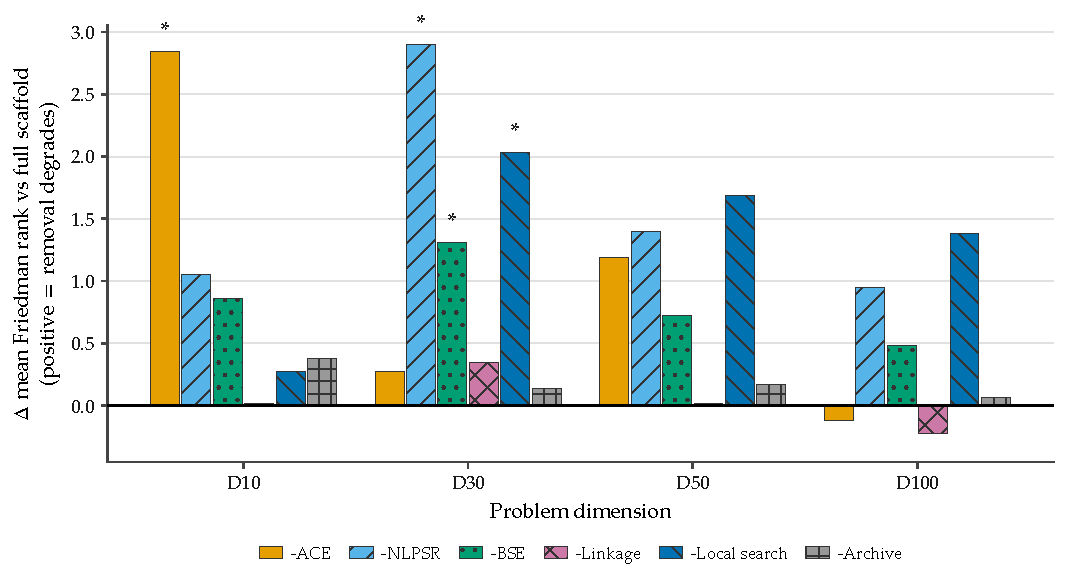
\includegraphics[width=0.92\textwidth]{figures/ablation/abl_rank_delta}
\caption{Conditional rank degradation from removing each scaffold component on
CEC2017 (\textbf{ISM off in every cell}; 51 runs; 29 functions).  Bars show
the change in mean Friedman rank versus the full-scaffold baseline; positive
means removing the component degrades rank.  Colours follow the frozen
per-cell palette; $\ast$ marks Holm-significant contrasts within a dimension
($\alpha = 0.05$).  Each bar is a conditional remove-one contribution, not an
independent causal effect, and bars are not averaged across dimensions.
}\label{fig:abl-rankdelta}
% BIND: X-ABL-01 (AB-01); ablation_matrix_rank_summary_cec2017_D{10,30,50,100}.csv; abl-rel-2026-07-20
\end{figure}

\begin{table}[H]
\caption{Scaffold remove-one ablation on CEC2017: full-vs-cell paired Wilcoxon
signed-rank test across the 29 functions~\cite{wilcoxon1945individual} with
Holm correction~\cite{holm1979simple} within each dimension's six-comparison
family ($\alpha = 0.05$), ordered by ascending raw $p$ within each dimension.
$\Delta$rank repeats the mean-rank change from Table~\ref{tab:abl-scaffold}.
Every contrast is a \emph{conditional} remove-one comparison with ISM off in
both cells and 51 runs per cell; the four Holm-significant results are all
\emph{favorable} (removing the component degrades performance).  }\label{tab:abl-wilcoxon}
% BIND: X-ABL-03 statistical family for X-ABL-01 (AB-01); Wilcoxon+Holm within dimension; abl-rel-2026-07-20
\centering
\tablesize{\footnotesize}
% AUTO-GENERATED by papers/scripts/generate_ablation_exhibits.py -- DO NOT EDIT BY HAND.
% Source (release-bound): papers/build_prompt_phases/phase_12/ablation_results/
% Promoted ablation release: benchmarks/cec_reference_results/_ablation/scaffold
% Study X-ABL-01 (scaffold remove-one); CEC2017; D10/30/50/100; 51 runs; 29 functions; ISM OFF in every cell.

\begin{tabular}{@{}lrrrc@{}}
\toprule
\textbf{Component removed} & \textbf{$\Delta$rank} & \textbf{Wilcoxon $p$} & \textbf{Holm $p$} & \textbf{Holm sig.} \\
\midrule
\multicolumn{5}{@{}l}{\textbf{$D=10$}\quad Friedman $p=1.8\times10^{-6}$; Holm family size $=6$} \\
\addlinespace[2pt]
-ACE & +2.84 & $1.84\times10^{-4}$ & 0.0011 & \textbf{yes} \\
-Local search & +0.28 & 0.044 & 0.219 & no \\
-BSE & +0.86 & 0.071 & 0.286 & no \\
-NLPSR & +1.05 & 0.226 & 0.678 & no \\
-Archive & +0.38 & 0.310 & 0.678 & no \\
-Linkage & +0.02 & 1.000 & 1.000 & no \\
\midrule
\multicolumn{5}{@{}l}{\textbf{$D=30$}\quad Friedman $p=2.5\times10^{-8}$; Holm family size $=6$} \\
\addlinespace[2pt]
-Local search & +2.03 & $2.41\times10^{-4}$ & 0.0014 & \textbf{yes} \\
-NLPSR & +2.90 & $8.77\times10^{-4}$ & 0.0044 & \textbf{yes} \\
-BSE & +1.31 & 0.0085 & 0.034 & \textbf{yes} \\
-Archive & +0.14 & 0.338 & 1.000 & no \\
-Linkage & +0.34 & 0.343 & 1.000 & no \\
-ACE & +0.28 & 0.648 & 1.000 & no \\
\midrule
\multicolumn{5}{@{}l}{\textbf{$D=50$}\quad Friedman $p=5.8\times10^{-3}$; Holm family size $=6$} \\
\addlinespace[2pt]
-BSE & +0.72 & 0.018 & 0.109 & no \\
-NLPSR & +1.40 & 0.025 & 0.123 & no \\
-Local search & +1.69 & 0.025 & 0.123 & no \\
-ACE & +1.19 & 0.054 & 0.163 & no \\
-Archive & +0.17 & 0.237 & 0.475 & no \\
-Linkage & +0.02 & 0.713 & 0.713 & no \\
\midrule
\multicolumn{5}{@{}l}{\textbf{$D=100$}\quad Friedman $p=3.5\times10^{-2}$; Holm family size $=6$} \\
\addlinespace[2pt]
-BSE & +0.48 & 0.061 & 0.368 & no \\
-Local search & +1.38 & 0.086 & 0.428 & no \\
-NLPSR & +0.95 & 0.125 & 0.499 & no \\
-Linkage & -0.22 & 0.697 & 1.000 & no \\
-ACE & -0.12 & 0.829 & 1.000 & no \\
-Archive & +0.07 & 0.856 & 1.000 & no \\
\bottomrule
\end{tabular}

\end{table}

\subsection{Findings (Conditional, ISM Off)}\label{sec:supp:ablation:findings}

% BIND: X-ABL-01 (AB-01); X-ABL-03 (Wilcoxon+Holm within dimension);
%   ablation_matrix_rank_summary_cec2017_D{10,30,50,100}.csv; abl-rel-2026-07-20
Across the four dimensions, only four of the twenty-four (cell, dimension)
contrasts survive Holm correction, and all four are \emph{favorable} ---
removing the named component degrades performance: ACE at $D=10$
(Holm $p = 1.1\times10^{-3}$) and, at $D=30$, the local search
(Holm $p = 1.4\times10^{-3}$), NLPSR (Holm $p = 4.4\times10^{-3}$), and the
budget-safe escape (Holm $p = 3.4\times10^{-2}$).  The per-mechanism
reading is dimension-structured:

% BIND: X-ABL-03 statistical family for X-ABL-01 (AB-01); per-mechanism rank
%   changes from ablation_matrix_rank_summary_cec2017_D{10,30,50,100}.csv; abl-rel-2026-07-20
\begin{itemize}
\item \textbf{ACE} is the low-dimensional backbone: the dominant and only
Holm-significant effect at $D=10$ (rank change $+2.84$), fading at mid
dimension and mildly \emph{negative} (non-significant) at $D=100$, where the
conditional delta's sign reverses.
\item \textbf{NLPSR} is the mid/upper-tier population backbone: the
largest and a Holm-significant degradation at $D=30$ (rank change $+2.90$)
and the second-largest at $D=50$ and $D=100$, though not Holm-significant
beyond $D=30$.
\item \textbf{Local search} is the most consistent mid/upper-tier
contributor: Holm-significant at $D=30$ and the single largest
degradation at both $D=50$ and $D=100$ (non-significant at either), but
negligible at $D=10$.
\item \textbf{BSE} yields a positive delta at every dimension ($+0.48$
to $+1.31$), Holm-significant at $D=30$.
\item \textbf{Linkage} and the \textbf{archive} are aggregate rank-neutral or
sign-mixed across dimensions (removing the linkage slightly \emph{improves}
rank at $D=100$); their conditional contribution has no stable sign, which is
why per-dimension reporting is mandatory and no dimension-averaged number is
quoted.
\end{itemize}

% BIND: X-ABL-01 (AB-01) D100 omnibus; X-ABL-03 (no contrast survives Holm at D100);
%   ablation_matrix_rank_summary_cec2017_D100.csv; abl-rel-2026-07-20
At $D=100$ the omnibus signal is weakest ($p = 2.7\times10^{-2}$) and
no contrast survives Holm; the $D=100$ ordering is descriptive only.  All six
disabled cells changed at least one function's per-run trajectory at every
dimension (active on 20--29 of 29 functions), so there are no null-contrast
cells and every contrast is identifiable.

\subsection{What This Study Does Not Establish}\label{sec:supp:ablation:limits}

The scaffold study is bounded on five axes, restated so that no reader
over-extends it.  (i)~It is ISM-off throughout and says nothing about the
interaction-structure memory.  (ii)~Its deltas are conditional, not causal,
and not additive.  (iii)~It covers one suite (CEC2017) and the four tested
dimensions only.  (iv)~The no\_arch and no\_bse couplings
above qualify two cells, and ARGP, the final polish, and the deep-stall
restart are untested here.  (v)~Aggregate ratios can be dominated by a few
functions and are never read alone.  Under the prespecified one-directional
correction guard, every favorable component result here is supplement-only and
does \emph{not} upgrade, strengthen, or convert any frozen main-text claim
(the main text defers all per-component attribution); no primary claim is
contradicted, and none is amended.

\subsection{ISM-Overlay Isolation: Direct Component Study}\label{sec:supp:ablation:sgsm}

The direct contribution of the interaction-structure memory is measured by a
\emph{separate} experimental design from the
scaffold matrix above, and is reported here.  Four ISM-active configurations
share one seed schedule (paired, common random numbers): the full overlay and
three single-toggle variants that disable, in turn, the interaction-structure
memory itself (no\_sgsm), its adaptive confidence gate
(no\_adaptive), and the ISM-dependent final polish
(no\_finalpolish).  Each cell runs $51$ paired repetitions ---
matching the primary panel's run count --- at the
overlay's active tiers, $D \in \{50, 100\}$, on the primary CEC2017 suite (and,
as a second suite, CEC2013 at $D = 50$).  Cells are compared on per-function
mean final error by a paired Wilcoxon signed-rank test across functions,
Holm-corrected over the prespecified three-comparison family, with Friedman
ranks over the four cells and Vargha--Delaney $A_{12}$ effect sizes computed
per function on the raw runs and averaged over functions; the four cells
differ overall (Iman--Davenport $F(3,84) = 5.59$,
$p = 1.5\times10^{-3}$; $F(3,84) = 4.87$, $p = 3.6\times10^{-3}$; and
$F(3,81) = 5.96$, $p = 1.0\times10^{-3}$ for CEC2017 $D50$, CEC2017 $D100$,
and CEC2013 $D50$).  These omnibus values use the tie-corrected Friedman
statistic with the Iman--Davenport $F$ --- the same decision criterion the
main text applies to the primary suites --- so component and primary
omnibus figures are now directly comparable.  The classical chi-square
approximation reported previously ($p = 2.4\times10^{-3}$,
$5.2\times10^{-3}$, and $3.8\times10^{-3}$) is retained as an audit
companion in the released contrasts files.  Because the tie-correction
factor satisfies $C \leq 1$, the correction can only increase the
statistic: every $p$-value decreases and no ranking or Holm decision in
this section changes.  The findings below are carried by the
Holm-corrected paired Wilcoxon tests of Table~\ref{tab:ism-isolation},
which the choice of omnibus statistic does not affect.
% BIND: X-ABL-02 overlay isolation; generate_ablation_matrix.py; _ablation/overlay evidence

\begin{table}[H]
\caption{Direct ISM-overlay isolation: the full overlay versus each
single-toggle cell, paired across functions and Holm-corrected. $\Delta$rank is
the Friedman mean-rank change when the mechanism is removed (lower rank is
better, so positive means removal \emph{hurts}); $A_{12} > 0.5$ favors the full
overlay.  Bold Holm $p < 0.05$.}\label{tab:ism-isolation}
\small\centering
\begin{tabular}{llccc}
\toprule
Suite ($D$) & Isolated mechanism & $\Delta$rank vs full & Holm $p$ & mean $A_{12}$\\
\midrule
CEC2017 ($50$)  & interaction-structure memory & $+0.05$ & $0.983$          & $0.51$\\
                & adaptive confidence gate     & $+0.47$ & $0.283$          & $0.51$\\
                & ISM-dependent final polish   & $+1.14$ & $\mathbf{0.002}$ & $0.59$\\
\addlinespace
CEC2017 ($100$) & interaction-structure memory & $+0.16$ & $0.897$          & $0.50$\\
                & adaptive confidence gate     & $+0.86$ & $0.079$          & $0.54$\\
                & ISM-dependent final polish   & $+0.98$ & $\mathbf{0.005}$ & $0.53$\\
\addlinespace
CEC2013 ($50$)  & interaction-structure memory & $+0.20$ & $0.647$          & $0.42$\\
                & adaptive confidence gate     & $+0.48$ & $0.235$          & $0.52$\\
                & ISM-dependent final polish   & $+1.18$ & $\mathbf{0.002}$ & $0.64$\\
\bottomrule
\end{tabular}
\end{table}
% BIND: benchmarks/cec_reference_results/_ablation/overlay/analysis/ablation_overlay_rank_summary_cec2017_D{50,100}.csv (CEC2017 D50/D100) + ablation_overlay_rank_summary_cec2013_D50.csv (CEC2013 D50); immutable release abl-rel-2026-07-20 (51-run rerun promoted 2026-07-16)

% BIND: X-ABL-02 overlay isolation; ablation_overlay_rank_summary_cec2017_D{50,100}.csv
%   + ablation_overlay_rank_summary_cec2013_D50.csv; ism_isolation_effects_cec2017.csv
%   + ism_isolation_effects_cec2013.csv (mean_a12; ism_runtime_overhead_pct); abl-rel-2026-07-20
Two findings are consistent across both tiers of the primary suite and the
second suite (Table~\ref{tab:ism-isolation}).  First, \textbf{the
interaction-structure memory shows no
significant standalone benefit at its active tiers}: disabling it moves the mean
rank negligibly (CEC2017 $\Delta$rank $= +0.05$ at $D50$ and $+0.16$ at $D100$),
the paired test is far from significance (Holm $p = 0.98$ and $0.90$), and the
effect size is essentially null ($A_{12} = 0.51$ and $0.50$); on CEC2013 the
rank delta is similarly negligible ($+0.20$) while the raw-run effect size
leans slightly toward the memory being off ($A_{12} = 0.42$).  Measured on the
corrected compiled backend (Section~\ref{sec:supp:ablation:caveats}), the
memory's wall-time cost is substantial at every active tier:
$\mathbf{{+}57.3\%}$ at CEC2017 $D50$, $\mathbf{{+}36.3\%}$ at $D100$, and
$+30.3\%$ on CEC2013 $D50$ --- so it costs a third to well over half again in
wall-clock and buys no measurable accuracy return.  Second,
\textbf{removing the complete final-polish phase changed performance
significantly in these cells} (Holm $p = 0.002$, $0.005$, $0.002$;
$A_{12} = 0.59$, $0.53$, $0.64$); the contrast removes the whole phase, so it
does not by itself attribute the effect among the phase's parts---the
basis-level attribution is provided by the direct isolation of
Section~\ref{sec:supp:rev:basis}---while the adaptive confidence gate helps directionally but not
significantly.  This corroborates the bundled-tier reading of the main text: the
upper-tier behavior is a property of the full tier configuration rather
than of the interaction-structure memory in isolation, and \dtgsk{}'s
family-best standing rests on the complete dimension-tiered system --- of whose
added mechanisms only the final polish carries an isolated, statistically
significant effect at these tiers (the no\_sgsm row is itself null, but it
disables the memory entirely --- removing its linkage channel as well as its
eigenbasis --- so it cannot separate the basis from the endgame;
Section~\ref{sec:supp:rev:basis} does that directly).  The interaction-structure memory's isolated
utility at $D \le 100$ therefore remains unestablished; whether its
structure-building role becomes decisive at larger scales is left to future work.
%==================================================================

%==================================================================
%==================================================================
\subsection{Conditional-Benefit Analysis by Function Class (Post-Hoc)}\label{sec:supp:ablation:subset}

The direct isolation above (Table~\ref{tab:ism-isolation}) returns a null for the
interaction-structure memory \emph{aggregated} over the CEC2017 functions.  Because a
coordinate-pair interaction memory should, if it helps at all, help most on functions
with genuine variable interaction, we ask \emph{post hoc} (this analysis was not
pre-registered) whether the aggregate null conceals a conditional benefit on those
functions.  We partition the 29 scored CEC2017 functions into the four standard
CEC2017 classes~\cite{awad2016problem} --- unimodal (F1, F3), simple multimodal
(F4--F10), hybrid (F11--F20), and composition (F21--F30) --- and, within each class,
count the per-function win/tie/loss of the full overlay against the memory-off
(no\_sgsm) cell (a win is a lower per-function mean error with the
interaction-structure memory on; tie at $|\Delta| < 10^{-8}$).  The hybrid and
composition functions, whose sub-component and rotation structure make variable
interaction explicit, are where such a memory should most plausibly help.

% BIND: Path-1 subset re-analysis of overlay_per_function_means_cec2017_D{50,100}.csv
%   (full vs no_sgsm), grouped by CEC2017 function class; read-only, no rerun; abl-rel-2026-07-20
\begin{table}[H]
\caption{Post-hoc conditional-benefit analysis: per-function win/tie/loss of the full
overlay versus the memory-off (no\_sgsm) cell, by CEC2017 function class, at
$D=50$ and $D=100$ (51 paired runs; a win is a lower per-function mean error with the
interaction-structure memory on).  Exploratory; not part of the pre-registered
isolation.}\label{tab:ism-subset}
\centering
\footnotesize
\begin{tabular}{lccc}
\toprule
\textbf{Function class} & \textbf{$n$} & \textbf{$D{=}50$ W/T/L (win-rate)} & \textbf{$D{=}100$ W/T/L (win-rate)}\\
\midrule
Unimodal (F1, F3)            & 2  & 2/0/0 (1.00) & 1/0/1 (0.50)\\
Simple multimodal (F4--F10)  & 7  & 3/0/4 (0.43) & 4/0/3 (0.57)\\
Hybrid (F11--F20)            & 10 & 7/0/3 (0.70) & 4/0/6 (0.40)\\
Composition (F21--F30)       & 10 & 3/0/7 (0.30) & 5/0/5 (0.50)\\
\midrule
Interacting (F11--F30)       & 20 & 10/0/10 (0.50) & 9/0/11 (0.45)\\
Non-interacting (F1--F10)    & 9  & 5/0/4 (0.56) & 5/0/4 (0.56)\\
All 29 (aggregate)           & 29 & 15/0/14 (0.52) & 14/0/15 (0.48)\\
\bottomrule
\end{tabular}
\end{table}

No class shows a benefit that survives even a nominal sign test (all subset
$p > 0.3$; the interacting-vs-non-interacting contrast is $0.50$ vs $0.56$ at $D=50$
and $0.45$ vs $0.56$ at $D=100$ --- the interacting classes never lead).  The only
favorable lean is on the
$D=50$ hybrids (win-rate $0.70$, median per-function $\log_{10}$-error gain $+0.026$),
and it reverses at $D=100$ (win-rate $0.40$, median $-0.002$); the
composition functions lean the other way at $D=50$ (win-rate $0.30$) and are flat
at $D=100$.  Together with the aggregate
Vargha--Delaney $A_{12}\approx 0.50$, the point estimates cluster on \emph{no}
average effect rather than on a small one --- though, absent a formal equivalence
test, this evidence is consistent with zero rather than establishing it.  The aggregate null is therefore not explained by the separable-problem
subset: no standalone benefit is detected even on the categories where variable
interaction is present by construction. This is a failure to detect an effect
under this design, not a demonstration that none exists.  We accordingly report the
interaction-structure memory as a controlled negative result on cheap accepted-move
structure-learning --- a boundary we believe is itself informative for the GSK family.
% BIND: Path-1 subset re-analysis of overlay_per_function_means_cec2017_D{50,100}.csv (full vs no_sgsm); read-only, no rerun


%==================================================================
\subsection{Implementation Caveats: Two Corrected Defects and Their Evidence Trail}\label{sec:supp:ablation:caveats}

A post-freeze code audit identified two implementation defects in the released
optimizer.  Both were disclosed, then \emph{fixed in the source} (each locked by a
regression test that fails on the pre-fix code), and the primary-panel, scaffold, and
overlay evidence in this paper was \textbf{fully regenerated with the corrected
binary at 51 runs per cell}; every number in the current release therefore reflects
the corrected implementation.  The two defects and their measured consequences are
recorded here for provenance.

% BIND: M038 (numba import path); ism_isolation_effects_cec2017.csv +
%   ism_isolation_effects_cec2013.csv, column ism_runtime_overhead_pct
%   (cec2017 D50 +57.3, D100 +36.3; cec2013 D50 +30.3) from
%   ablation_overlay_effects.py over the 51-run overlay per_run.csv runtime_seconds;
%   the pre-fix +54%/+37% are historical and superseded. Backend FP-identity: M040.
\paragraph{The interaction graph's compiled kernels were silently disabled in the
pre-fix runs.}
The interaction graph ships compiled (numba) kernels alongside \textsc{NumPy}
reference implementations, guarded by an import that silently falls back to
\textsc{NumPy} if the compiled module is unavailable.  In the pre-fix configuration
that import named the wrong module path, so the earlier runs executed the
\textsc{NumPy} path throughout.  The compiled kernels are built without fast-math and
without thread-parallel reduction precisely so that they reproduce the \textsc{NumPy}
arithmetic exactly, and we confirmed bit-identical optimization results across both
backends --- the defect inflated wall-clock only.  The overhead and runtime figures
in this paper (Section~\ref{sec:supp:ablation:sgsm} and the main-text runtime table)
were re-measured with the compiled kernels active over the full 51-run overlay:
the memory's wall-time cost is $+57.3\%$ at CEC2017 $D50$, $+36.3\%$ at $D100$,
and $+30.3\%$ on CEC2013 $D50$. These are close to the $+54\%$/$+37\%$ recorded
before the backend fix, which is expected rather than surprising: the compiled
kernels accelerated the memory-on and memory-off arms alike, so the \emph{ratio}
between them barely moved. The fix removed a wall-clock inflation common to both
arms; it did not make the interaction-structure memory cheaper relative to
running without it.

\paragraph{The final polish previously refined a one-generation-stale incumbent.}
In the pre-fix binary, the eigenframe polish was invoked with the incumbent
materialized at the end of the \emph{previous} generation, and its accept test
compared against that same stale value --- so the polish could start from, and
accept against, a point the current generation had already improved upon.  Reported
results were protected throughout by a best-ever shadow (no run could report a value
worse than the best it found), so this was a loss of polish \emph{effectiveness},
never a correctness defect.  The fix re-materializes the incumbent atomically at
polish entry.  The isolation reported above therefore measures the polish
\emph{un-handicapped}; its contribution remains Holm-significant on every suite and
tier, and the headline panel ranks are unchanged relative to the pre-fix release ---
the correction altered $D \geq 50$ trajectories without flipping any per-function
panel ordering.

%==================================================================
% S7 -- CEC2013LSGO large-scale suite (Phase W2). Every value below is
% machine-transcribed from the committed analysis bundle
% papers/analysis/lsgo-rel-2026-07-28-ff1a046ef/cec2013lsgo/ by
% w2_gen_s7s8.py; the registered tiers follow the pre-registered SAP
% addendum (signing commit 5c9bfae82) and its dated Amendments 1-2.
%==================================================================
\section{CEC2013LSGO Large-Scale Suite}\label{sec:supp:cec2013lsgo}

\subsection{Protocol, Evidential Tiers, and Scope}\label{sec:supp:lsgo:protocol}

\noindent CEC2013LSGO is the large-scale suite of this study, reported as a
family-internal comparison at the suite's native scale: 15 functions at
$D = 1000$, with the two overlapping functions F13 and F14 at their native
$D = 905$; 25 runs per function; a budget of $3 \times 10^{6}$ function
evaluations per run; and the same seven-algorithm family panel and unified
seed schedule (base seed 20240620) used throughout this
paper~\cite{li2013lsgo}.  Statistics on this suite use the raw best
objective value (CEC2011-style; the suite's error column is not populated),
so magnitudes are not comparable across functions and no error floor is
applied.  One benchmark-implementation disclosure governs every F3, F6 and
F10 value: those functions ran the \emph{transformed} Ackley variant, so
results on them are not comparable to published values obtained on the raw
variant, and no such comparison is drawn anywhere in this paper.
Every number in this section derives from the separate, non-superseding
evidence release lsgo-rel-2026-07-28-ff1a046ef and its committed analysis
bundle; the primary evidence release rel-2026-07-20-67d9345f9 is untouched
by this suite.
% BIND: RS-13; addendum Section 2; benchmark_variant.json sidecars (D-8.2);
% descriptive_stats_cec2013lsgo_native.csv (15 functions, dims 1000/905, 25 runs);
% evidence_release_manifest_cec2013lsgo.json (release_id)

Two evidential tiers apply, fixed by the pre-registered analysis-plan
addendum (statistical\_analysis\_plan\_addendum\_cec2020\_lsgo.md), signed
before any result existed and binding on every sentence of this section.
Before the addendum was signed, the family-only Friedman mean ranks, the
omnibus, the Nemenyi view and the per-function win/loss descriptives of
this suite had been informally inspected; the addendum's Section~6
declares that exposure verbatim.  Those quantities are therefore reported
here as \emph{descriptive-after-inspection}: they carry no confirmatory
weight and enter no headline.  The run-level paired Wilcoxon layer and the
effect-size layer had never been computed when the addendum was signed;
they were registered there, before computation, as the confirmatory LSGO
layer, and their first computations are recorded in the addendum's dated
Amendments 1 and 2.
% BIND: addendum Section 6 (prior-inspection disclosure); amendments 1 (A1.3) and 2 (A2.1)

The CEC2013LSGO analysis in this paper is family-internal: it ranks the
seven GSK-family variants against one another under a common protocol.
Dedicated large-scale optimizers --- for example
SHADE-ILS~\cite{molina2018shadeils} and MOS~\cite{latorre2013mos} ---
report substantially stronger published results on this suite than any
GSK-family member, and no competitiveness with such specialists is claimed
here; cross-paradigm comparison is outside this paper's scope.
% BIND: disclosure sentence (a), FINAL_PUBLICATION_PLAN 0.4, adopted 2026-07-28 (verbatim); LM-06; RS-13
For completeness: the public repository cited in the Data Availability
Statement additionally holds exploratory first-party ports of SHADE-ILS, MOS
and DECC-G, executed on this suite under the same harness and seed schedule.
They are retained there as exploratory material outside the registered
panel; they are not analysed in this paper, they enter no ranking or test
reported here, and no claim in this paper rests on them.

\subsection{Configuration Provenance on This Suite}\label{sec:supp:lsgo:config}

\dtgsk{} runs the same hash-frozen configuration here as on the
bound-constrained suites, with one disclosed exception that exists for no
other suite: the shipped dimension-tier table does not extend to the
suite's native $D = 905$ and $D = 1000$, so two linkage-block-size entries
($905 \rightarrow 50$ and $1000 \rightarrow 50$) were added for this
suite alone, while all six comparators ran with empty optimizer options.
A second configuration asymmetry is disclosed here because it is larger on
this suite than anywhere else in the paper: \dtgsk{}'s
$NP_{\mathrm{init}} = 5D$ rule gives $5{,}000$ individuals at $D = 1000$
against the comparators' reference-implementation value of $100$ --- a
fifty-fold ratio at initialization, where the corresponding ratio is
five-fold at $D = 100$ on the bound-constrained suites. The budget is
equalized on function evaluations rather than on population size, so the
larger initial population buys proportionally fewer generations; the
population rule is not a controlled variable on this suite, and the
matched-population control of Section~\ref{sec:supp:rev:np} covers
CEC2017 only.
The value 50 follows a structural rule recorded in the configuration file
at the time the entries were introduced: it matches the benchmark's own
declared group structure --- the suite builds its partially separable
functions from groups of 25, 50 and 100 variables, with F8--F11 using
twenty groups of 50 and F13/F14 using 50-dimensional overlapping groups
--- rather than any observed result, and no parameter search was run.
The timing is disclosed rather than glossed: the two entries were added on
2026-07-24, while \dtgsk{} CEC2013LSGO results had existed in the
repository since 2026-07-21, so outcome-blindness is not asserted for
them.  What is asserted is the stated structural rule, its contemporaneous
record in the configuration file, and the absence of any parameter
search; the registered run-level layer below, which found no suite-level
separation in \dtgsk{}'s favor against any comparator, is not inflated
by this choice.
% BIND: production_deviation_record.md D-8.4 (values 2026-07-24, commit 4d5c8dad4;
% results since 2026-07-21, a11641bde; configs/dtgsk_cec2013lsgo.yml rationale comment)

\subsection{Family Friedman and Nemenyi View (Descriptive After Inspection)}\label{sec:supp:lsgo:ranks}

The registered standing statement for this suite is quoted from the
addendum's pre-committed wording bank: \dtgsk{} and \agsk{} share the
best descriptive family mean rank (both 3.1333, tied-first); no member
except \egsk{} (worse) is separable by the omnibus procedure; and
\dtgsk{} is last on F7 and F15.  Table~\ref{tab:supp:lsgo:ranks} gives
the full view.  The tie-corrected Friedman omnibus over the 15 function
blocks gives $\chi^{2} = 15.314$ (df 6, tie correction $C = 1.0$, no tied
blocks), Iman--Davenport $F(6, 84) = 2.8707$, $p = 0.0136$; the Nemenyi
critical distance at $\alpha = 0.05$ is $2.326$ ($k = 7$, $N = 15$),
which separates only \egsk{} from the two tied-first members.  Under the
registered tier this entire subsection is descriptive-after-inspection:
it carries no confirmatory weight, and the mandatory median-basis re-rank
of the registered robustness family reproduces every ordinal, the
registered relative-tie-band variant leaves every win/tie/loss split
unchanged on the raw basis, while the
leave-one-function-out variant --- registered as exploratory because the
F7/F15 deletions are inspection-informed --- moves some ordinals and is
recorded in full in the released robustness digest.
% BIND: AN-OMNI-LSGO-NATIVE (friedman_ranks_cec2013lsgo_native.csv);
% AN-ROB-LSGO (robustness/robustness_cec2013lsgo.csv: mean_vs_median all agree,
% relative_tie_band all agree, loo_* exploratory); addendum Sections 6 and 9

\begin{table}[H]
\caption{CEC2013LSGO family-only tie-corrected Friedman mean ranks over
the 15 function blocks (native $D = 1000$; F13/F14 at $D = 905$; 25 runs;
raw best-objective basis) with the Nemenyi critical distance
$\mathrm{CD} = 2.326$ ($k = 7$, $N = 15$, $\alpha = 0.05$).  Lower rank
is better; \dtgsk{} and \agsk{} are exactly tied-first.  Evidential
tier: descriptive-after-inspection (addendum Section~6) --- these ranks
were informally inspected before the analysis plan was signed, carry no
confirmatory weight, and enter no confirmatory headline.
}\label{tab:supp:lsgo:ranks}
% BIND: AN-OMNI-LSGO-NATIVE (friedman_ranks_cec2013lsgo_native.csv;
% nemenyi_cd_cec2013lsgo_native.csv)
\centering
\tablesize{\footnotesize}
\zebra
\begin{tabular}{lcc}
\toprule
\textbf{Algorithm} & \textbf{Mean rank} & \textbf{Ordinal} \\
\midrule
GSK & 3.8667 & 4 \\
AGSK & 3.1333 & 1 (tied-first) \\
APGSK & 4.9333 & 6 \\
FDB-AGSK & 3.9333 & 5 \\
ATMALS-GSK & 3.5333 & 3 \\
eGSK & 5.4667 & 7 \\
DT-GSK & 3.1333 & 1 (tied-first) \\
\bottomrule
\end{tabular}
\end{table}

\subsection{Across-Function Wilcoxon (Supporting, With Disclosure)}\label{sec:supp:lsgo:pairwise}

Table~\ref{tab:supp:lsgo:wilcoxon} reports the across-function Wilcoxon
signed-rank layer: \dtgsk{} against each comparator on the 15 paired
per-function means of the raw best objective, decided by exact sign-flip
enumeration over all $2^{15}$ patterns, with the normal-approximation $p$
recorded alongside for continuity with the frozen suites and Holm
correction over the $m = 6$ comparators.  No comparator separates from
\dtgsk{} at $\alpha = 0.05$ after Holm --- the smallest Holm-adjusted
$p$ is 0.2875 (\apgsk{} and \egsk{}) --- so this layer demonstrates no
separation in either direction; in particular, paired tests do not
separate \dtgsk{} from \agsk{} (exact $p = 0.8469$, Holm-adjusted $1.0$).
Per the addendum's pre-committed power disclosure, these $N = 15$
across-function families are low-powered by construction (Nemenyi
critical distance $2.326$ against $1.673$ at the $N = 29$ CEC2017
families), so non-significance on this suite is read as no separation
demonstrated, never as equivalence.
% BIND: AN-PW-LSGO-NATIVE (wilcoxon_holm_cec2013lsgo_native.csv); amendment 1 A1.3; addendum Section 7 (power disclosure)

\begin{table}[H]
\caption{Across-function Wilcoxon signed-rank layer on CEC2013LSGO,
\dtgsk{} vs.\ each family comparator ($n = 15$ paired per-function
means of the raw best objective over 25 runs; zero differences
$|\Delta| < 10^{-8}$ discarded before ranking --- none occurred,
$n_{\mathrm{eff}} = 15$ throughout).  The decision $p$ is the exact
two-sided sign-flip enumeration over all $2^{15}$ signed-rank patterns;
the normal-approximation $p$ is recorded for continuity with the frozen
suites; Holm step-down is applied over the six comparators.  W--L is the
per-function mean win--loss split for \dtgsk{}.  No comparison is
Holm-significant: this layer demonstrates no separation in either
direction.  Evidential tier: supporting-with-disclosure (addendum
Section~4).
}\label{tab:supp:lsgo:wilcoxon}
% BIND: AN-PW-LSGO-NATIVE (wilcoxon_holm_cec2013lsgo_native.csv)
\centering
\tablesize{\footnotesize}
\zebra
\begin{tabular}{lccccc}
\toprule
\textbf{Comparator} & \textbf{W--L} & \textbf{$p$ (exact)} &
\textbf{$p$ (normal)} & \textbf{$p$ (Holm)} & \textbf{Decision} \\
\midrule
GSK & 8--7 & 0.7615 & 0.7548 & 1.0000 & no separation \\
AGSK & 9--6 & 0.8469 & 0.8424 & 1.0000 & no separation \\
APGSK & 11--4 & 0.0554 & 0.0571 & 0.2875 & no separation \\
FDB-AGSK & 11--4 & 0.0833 & 0.0832 & 0.3330 & no separation \\
ATMALS-GSK & 8--7 & 0.1688 & 0.1641 & 0.5065 & no separation \\
eGSK & 11--4 & 0.0479 & 0.0501 & 0.2875 & no separation \\
\bottomrule
\end{tabular}
\end{table}

\subsection{Run-Level Paired Wilcoxon (Registered Confirmatory Layer)}\label{sec:supp:lsgo:runlevel}

Table~\ref{tab:supp:lsgo:runlevel} reports the registered confirmatory
layer: per-function run-level Wilcoxon over the 25 seed-paired runs
(pairing key = run id; seed identity across all seven algorithms verified
with zero mismatches), exact two-sided $p$, Holm-corrected \emph{across
the 15 functions} per comparator ($m = 15$); as registered, no additional
correction is applied across the six comparators, so the six columns are
not jointly error-controlled and are never summed into one claim.  Two
cross-comparator regularities are stated in both directions: \dtgsk{} is
Holm-significantly \emph{better} than every family member on F4 and F8,
and Holm-significantly \emph{worse} than every family member on F7 and
F15.  Per comparator, the Holm-significant win/loss/no-separation counts
are 8/6/1 vs.\ GSK; 9/6/0 vs.\ AGSK; 11/3/1 vs.\ APGSK; 11/4/0 vs.\ FDB-AGSK; 7/6/2 vs.\ ATMALS-GSK; 11/4/0 vs.\ eGSK.
The binding suite-level wording, fixed by the addendum's Section~9 before
this layer was ever computed, applies verbatim: tied-first descriptive
rank; paired tests do not separate \dtgsk{} from \agsk{}.
% BIND: AN-PWRUN-LSGO-NATIVE (wilcoxon_run_cec2013lsgo_native.csv);
% amendment 1 A1.3 (first computation); addendum Section 9 (binding wording)

\begin{table}[p]
\caption{Registered confirmatory layer on CEC2013LSGO: per-function
run-level Wilcoxon over the 25 seed-paired runs, \dtgsk{} vs.\ each
family comparator, exact two-sided $p$ Holm-corrected across the 15
functions per comparator ($m = 15$; no correction across comparators, as
registered).  Cell entries are the Holm-significant outcome for \dtgsk{}
(W = win, L = loss, n.s.\ = no separation demonstrated) with the
Holm-adjusted $p$.  Zero differences $|\Delta| < 10^{-8}$ are discarded
($n_{\mathrm{eff}} = 25$ in every cell).  \dtgsk{} wins F4 and F8
against every comparator and loses F7 and F15 against every comparator.
Evidential tier: confirmatory-with-disclosure (addendum Sections 3--4;
never computed before registration).
}\label{tab:supp:lsgo:runlevel}
% BIND: AN-PWRUN-LSGO-NATIVE (wilcoxon_run_cec2013lsgo_native.csv)
\centering
\tablesize{\footnotesize}
\resizebox{\textwidth}{!}{%
\zebra
\begin{tabular}{lcccccc}
\toprule
\textbf{Func.} & \textbf{GSK} & \textbf{AGSK} & \textbf{APGSK} & \textbf{FDB-AGSK} & \textbf{ATMALS-GSK} & \textbf{eGSK} \\
\midrule
F1 & L 0.0202 & L 3.02E-05 & W 8.94E-07 & W 8.94E-07 & L 8.94E-07 & W 8.94E-07 \\
F2 & W 8.94E-07 & W 8.94E-07 & W 8.94E-07 & L 3.61E-04 & L 8.94E-07 & W 8.94E-07 \\
F3 & W 8.94E-07 & W 8.94E-07 & W 8.94E-07 & W 4.17E-06 & L 8.94E-07 & W 0.0160 \\
F4 & W 8.94E-07 & W 8.94E-07 & W 8.94E-07 & W 8.94E-07 & W 8.94E-07 & W 8.94E-07 \\
F5 & L 8.94E-07 & W 8.94E-07 & W 8.94E-07 & W 8.94E-07 & W 3.27E-05 & L 1.07E-04 \\
F6 & W 2.38E-06 & W 2.09E-06 & W 8.94E-07 & W 1.79E-06 & n.s. 0.1334 & W 1.62E-04 \\
F7 & L 8.94E-07 & L 8.94E-07 & L 8.94E-07 & L 8.94E-07 & L 8.94E-07 & L 8.94E-07 \\
F8 & W 8.94E-07 & W 8.94E-07 & W 8.94E-07 & W 8.94E-07 & W 8.94E-07 & W 8.94E-07 \\
F9 & L 8.94E-07 & W 8.94E-07 & W 8.94E-07 & W 8.94E-07 & W 2.98E-06 & L 0.0029 \\
F10 & W 8.94E-07 & W 0.0036 & n.s. 0.5424 & W 0.0056 & W 9.58E-05 & W 8.94E-07 \\
F11 & n.s. 0.9158 & L 1.67E-05 & W 8.94E-07 & W 0.0056 & W 8.94E-07 & W 8.94E-07 \\
F12 & W 8.94E-07 & W 8.94E-07 & W 8.94E-07 & W 8.94E-07 & L 8.94E-07 & W 8.94E-07 \\
F13 & L 0.0473 & L 8.94E-07 & L 0.0023 & L 8.94E-07 & n.s. 0.8325 & W 8.94E-07 \\
F14 & W 8.94E-07 & L 0.0038 & W 8.94E-07 & W 8.94E-07 & W 8.94E-07 & W 8.94E-07 \\
F15 & L 8.94E-07 & L 8.94E-07 & L 9.83E-06 & L 1.67E-05 & L 8.94E-07 & L 8.94E-07 \\
\bottomrule
\end{tabular}}
\end{table}

\subsection{Effect Sizes}\label{sec:supp:lsgo:effects}

Table~\ref{tab:supp:lsgo:effects} reports the registered effect-size
layer: run-level $A_{12}$ and Cliff's $\delta$ over the 25 seed-paired
runs per cell, with BCa 95\% confidence intervals ($B = 10{,}000$) on
the paired mean differences released in the analysis bundle.  All 90
cells are non-degenerate ($n_{\mathrm{eff}} = 25$ everywhere).  Effects
are bimodal rather than graded: 86 of 90 cells are large, and 52 are
saturated at $A_{12}$ exactly $0$ or $1$ (complete sample separation);
85 of the 90 BCa intervals exclude zero.  F4 and F8 are complete
separations in \dtgsk{}'s favor against all six comparators; F7 and F15
are near-complete separations against it.  Mean $A_{12}$ by comparator is
0.5885 vs.\ GSK, 0.6097 vs.\ AGSK, 0.7830 vs.\ APGSK, 0.7060 vs.\ FDB-AGSK, 0.4988 vs.\ ATMALS-GSK, 0.7261 vs.\ eGSK.
Against \atmals{} the mean effect favors the comparator (mean Cliff's
$\delta = -0.0025$): no superiority over \atmals{} on this suite is
supportable from the effect layer.  One divergence of estimand, not of
direction, is disclosed rather than suppressed: on F1 vs.\ GSK,
$A_{12} = 0.1456$ (large, favoring GSK) while the BCa interval on the
paired mean difference straddles zero (mean difference $2.40 \times 10^{6}$,
interval $[-1.80 \times 10^{6}, 4.23 \times 10^{6}]$), because F1's raw
distribution is heavy-tailed; both are reported.
% BIND: AN-EFF-LSGO-NATIVE (effect_sizes_cec2013lsgo_native.csv:
% 86/90 large, 52/90 saturated, mean A12 per comparator;
% bca_ci_cec2013lsgo_native.csv: 85/90 exclude zero, F1-vs-gsk interval);
% amendment 2 A2.1 (first computation)

\begin{table}[p]
\caption{Run-level effect sizes on CEC2013LSGO: $A_{12}$/Cliff's
$\delta$ for \dtgsk{} against each family comparator on each function
(25 seed-paired runs; tie band $|\Delta| < 10^{-8}$ counted half;
$A_{12} > 0.5$ and $\delta > 0$ favor \dtgsk{}).  BCa 95\% intervals
($B = 10{,}000$) on the paired mean differences accompany every cell in
the released bundle; no cell is degenerate.  Saturated cells ($A_{12}$
exactly $0.00$ or $1.00$) are complete sample separations.
}\label{tab:supp:lsgo:effects}
% BIND: AN-EFF-LSGO-NATIVE (effect_sizes_cec2013lsgo_native.csv;
% bca_ci_cec2013lsgo_native.csv)
\centering
\tablesize{\footnotesize}
\resizebox{\textwidth}{!}{%
\zebra
\begin{tabular}{lcccccc}
\toprule
\textbf{Func.} & \textbf{GSK} & \textbf{AGSK} & \textbf{APGSK} & \textbf{FDB-AGSK} & \textbf{ATMALS-GSK} & \textbf{eGSK} \\
\midrule
F1 & 0.15/-0.71 & 0.12/-0.75 & 1.00/1.00 & 1.00/1.00 & 0.00/-1.00 & 1.00/1.00 \\
F2 & 1.00/1.00 & 1.00/1.00 & 1.00/1.00 & 0.13/-0.73 & 0.00/-1.00 & 1.00/1.00 \\
F3 & 1.00/1.00 & 1.00/1.00 & 1.00/1.00 & 0.90/0.80 & 0.00/-1.00 & 0.72/0.44 \\
F4 & 1.00/1.00 & 1.00/1.00 & 1.00/1.00 & 1.00/1.00 & 1.00/1.00 & 1.00/1.00 \\
F5 & 0.00/-1.00 & 1.00/1.00 & 1.00/1.00 & 1.00/1.00 & 0.89/0.79 & 0.11/-0.78 \\
F6 & 0.96/0.92 & 0.95/0.90 & 0.95/0.90 & 0.98/0.96 & 0.34/-0.31 & 0.84/0.68 \\
F7 & 0.00/-1.00 & 0.00/-1.00 & 0.00/-1.00 & 0.00/-1.00 & 0.00/-1.00 & 0.03/-0.94 \\
F8 & 1.00/1.00 & 1.00/1.00 & 1.00/1.00 & 1.00/1.00 & 1.00/1.00 & 1.00/1.00 \\
F9 & 0.00/-0.99 & 1.00/1.00 & 1.00/1.00 & 1.00/1.00 & 0.90/0.79 & 0.21/-0.57 \\
F10 & 0.98/0.97 & 0.78/0.56 & 0.41/-0.17 & 0.81/0.62 & 0.86/0.71 & 0.97/0.95 \\
F11 & 0.45/-0.10 & 0.06/-0.88 & 1.00/1.00 & 0.72/0.45 & 1.00/0.99 & 1.00/1.00 \\
F12 & 1.00/1.00 & 1.00/1.00 & 1.00/1.00 & 1.00/1.00 & 0.00/-1.00 & 1.00/1.00 \\
F13 & 0.28/-0.43 & 0.00/-1.00 & 0.25/-0.50 & 0.01/-0.98 & 0.49/-0.01 & 1.00/1.00 \\
F14 & 1.00/1.00 & 0.23/-0.55 & 1.00/1.00 & 0.93/0.86 & 1.00/1.00 & 1.00/1.00 \\
F15 & 0.00/-1.00 & 0.00/-1.00 & 0.13/-0.74 & 0.11/-0.78 & 0.00/-1.00 & 0.01/-0.99 \\
\bottomrule
\end{tabular}}
\end{table}

\subsection{Per-Function Detail}\label{sec:supp:lsgo:detail}

Tables~\ref{tab:supp:lsgo-detail-a} and \ref{tab:supp:lsgo-detail-b}
report the five-statistic per-function record (best / median / mean /
worst / SD of the raw best objective over the 25 runs) for all seven
family algorithms on all 15 functions.  As everywhere on this suite, the
basis is the raw best objective; the F3, F6 and F10 rows are
transformed-Ackley values, not comparable to published raw-Ackley
numbers.
% BIND: descriptive_stats_cec2013lsgo_native.csv (105 rows = 15 x 7)

\begin{table}[p]
\caption{CEC2013LSGO per-function detail (F1--F8): best / median / mean /
worst / SD of the raw best objective over 25 runs for all 7 GSK-family
algorithms at the native dimension ($D = 1000$; F13/F14 at $D = 905$);
best mean per function in bold (ties all bold).  F3, F6 and F10 ran the
transformed Ackley variant and are not comparable to published
raw-Ackley values.
}\label{tab:supp:lsgo-detail-a}
% BIND: descriptive_stats_cec2013lsgo_native.csv
\centering
\tablesize{\scriptsize}
\resizebox{\textwidth}{!}{%
\zebra
\begin{tabular}{llrrrrrrr}
\toprule
\textbf{Func.} & \textbf{Stat.} & \textbf{GSK} & \textbf{AGSK} & \textbf{APGSK} & \textbf{FDB-AGSK} & \textbf{ATMALS-GSK} & \textbf{eGSK} & \textbf{DT-GSK} \\
\midrule
F1 & Best & 6.70E+05 & 5.40E+05 & 1.52E+07 & 1.06E+07 & 1.01E+04 & 2.00E+07 & 4.39E+06 \\
 & Median & 1.74E+06 & 2.25E+06 & 5.33E+07 & 3.62E+07 & 2.14E+04 & 9.23E+07 & 6.26E+06 \\
 & Mean & 4.24E+06 & 3.00E+06 & 9.61E+07 & 5.96E+07 & \bestval{2.16E+04} & 3.26E+08 & 6.64E+06 \\
 & Worst & 3.46E+07 & 7.58E+06 & 3.90E+08 & 3.14E+08 & 4.30E+04 & 1.40E+09 & 9.76E+06 \\
 & SD & 7.22E+06 & 2.23E+06 & 1.01E+08 & 6.88E+07 & 8.18E+03 & 4.12E+08 & 1.63E+06 \\
\midrule
F2 & Best & 2.01E+04 & 1.25E+04 & 1.48E+04 & 6.46E+03 & 3.48E+02 & 2.45E+04 & 9.08E+03 \\
 & Median & 2.15E+04 & 1.31E+04 & 1.59E+04 & 7.95E+03 & 4.08E+02 & 2.87E+04 & 9.79E+03 \\
 & Mean & 2.16E+04 & 1.32E+04 & 1.59E+04 & 8.34E+03 & \bestval{4.11E+02} & 2.84E+04 & 9.70E+03 \\
 & Worst & 2.31E+04 & 1.38E+04 & 1.68E+04 & 1.32E+04 & 4.61E+02 & 3.08E+04 & 1.01E+04 \\
 & SD & 7.30E+02 & 3.39E+02 & 5.08E+02 & 1.38E+03 & 3.09E+01 & 1.80E+03 & 3.11E+02 \\
\midrule
F3 & Best & 2.16E+01 & 2.13E+01 & 2.13E+01 & 2.04E+01 & 2.00E+01 & 2.03E+01 & 2.05E+01 \\
 & Median & 2.16E+01 & 2.13E+01 & 2.13E+01 & 2.11E+01 & 2.00E+01 & 2.06E+01 & 2.05E+01 \\
 & Mean & 2.16E+01 & 2.13E+01 & 2.13E+01 & 2.10E+01 & \bestval{2.00E+01} & 2.06E+01 & 2.05E+01 \\
 & Worst & 2.16E+01 & 2.14E+01 & 2.13E+01 & 2.13E+01 & 2.00E+01 & 2.08E+01 & 2.06E+01 \\
 & SD & 8.06E-03 & 7.82E-03 & 6.12E-03 & 2.81E-01 & 8.36E-04 & 1.10E-01 & 2.29E-02 \\
\midrule
F4 & Best & 1.30E+10 & 3.44E+09 & 1.01E+10 & 7.48E+09 & 1.42E+10 & 5.28E+10 & 1.05E+09 \\
 & Median & 2.88E+10 & 5.94E+09 & 1.66E+10 & 1.17E+10 & 3.68E+10 & 8.28E+10 & 1.36E+09 \\
 & Mean & 3.34E+10 & 6.50E+09 & 1.71E+10 & 1.32E+10 & 3.98E+10 & 9.40E+10 & \bestval{1.41E+09} \\
 & Worst & 7.77E+10 & 1.16E+10 & 3.39E+10 & 2.11E+10 & 8.69E+10 & 1.90E+11 & 1.91E+09 \\
 & SD & 1.51E+10 & 2.14E+09 & 4.83E+09 & 4.18E+09 & 1.79E+10 & 3.92E+10 & 2.37E+08 \\
\midrule
F5 & Best & 1.32E+06 & 5.81E+06 & 9.89E+06 & 3.34E+06 & 2.53E+06 & 1.47E+06 & 2.29E+06 \\
 & Median & 1.82E+06 & 6.79E+06 & 1.07E+07 & 6.75E+06 & 3.62E+06 & 2.23E+06 & 2.72E+06 \\
 & Mean & \bestval{1.82E+06} & 6.83E+06 & 1.07E+07 & 6.54E+06 & 3.61E+06 & 2.14E+06 & 2.71E+06 \\
 & Worst & 2.24E+06 & 7.82E+06 & 1.19E+07 & 8.57E+06 & 5.29E+06 & 3.03E+06 & 3.31E+06 \\
 & SD & 2.66E+05 & 5.38E+05 & 5.47E+05 & 1.04E+06 & 6.93E+05 & 4.13E+05 & 2.62E+05 \\
\midrule
F6 & Best & 1.06E+06 & 1.06E+06 & 1.06E+06 & 1.06E+06 & 1.05E+06 & 1.05E+06 & 1.04E+06 \\
 & Median & 1.06E+06 & 1.06E+06 & 1.06E+06 & 1.06E+06 & 1.05E+06 & 1.06E+06 & 1.06E+06 \\
 & Mean & 1.06E+06 & 1.06E+06 & 1.06E+06 & 1.06E+06 & \bestval{1.05E+06} & 1.06E+06 & 1.05E+06 \\
 & Worst & 1.06E+06 & 1.06E+06 & 1.06E+06 & 1.06E+06 & 1.06E+06 & 1.06E+06 & 1.06E+06 \\
 & SD & 1.35E+03 & 1.12E+03 & 1.34E+03 & 1.14E+03 & 3.11E+03 & 1.93E+03 & 3.91E+03 \\
\midrule
F7 & Best & 9.42E+06 & 6.70E+06 & 3.07E+07 & 1.48E+07 & 2.44E+07 & 2.33E+07 & 1.11E+08 \\
 & Median & 2.81E+07 & 1.30E+07 & 4.09E+07 & 2.59E+07 & 4.88E+07 & 4.33E+07 & 1.67E+08 \\
 & Mean & 3.05E+07 & \bestval{1.47E+07} & 4.20E+07 & 2.85E+07 & 5.00E+07 & 5.21E+07 & 1.76E+08 \\
 & Worst & 9.86E+07 & 2.77E+07 & 5.87E+07 & 5.01E+07 & 8.74E+07 & 1.86E+08 & 3.29E+08 \\
 & SD & 1.85E+07 & 5.58E+06 & 8.22E+06 & 1.05E+07 & 1.68E+07 & 3.45E+07 & 4.41E+07 \\
\midrule
F8 & Best & 2.71E+11 & 8.47E+12 & 1.55E+13 & 1.11E+13 & 1.99E+13 & 2.29E+13 & 2.37E+10 \\
 & Median & 6.98E+12 & 2.89E+13 & 5.33E+13 & 3.79E+13 & 4.01E+13 & 8.41E+13 & 3.43E+10 \\
 & Mean & 9.69E+12 & 3.57E+13 & 6.04E+13 & 4.70E+13 & 5.41E+13 & 9.66E+13 & \bestval{3.42E+10} \\
 & Worst & 3.35E+13 & 9.53E+13 & 1.23E+14 & 1.34E+14 & 2.46E+14 & 3.30E+14 & 4.51E+10 \\
 & SD & 8.90E+12 & 2.24E+13 & 3.12E+13 & 2.90E+13 & 4.61E+13 & 6.28E+13 & 5.51E+09 \\
\bottomrule
\end{tabular}}
\end{table}

\begin{table}[p]
\caption{CEC2013LSGO per-function detail (F9--F15): best / median / mean /
worst / SD of the raw best objective over 25 runs for all 7 GSK-family
algorithms at the native dimension ($D = 1000$; F13/F14 at $D = 905$);
best mean per function in bold (ties all bold).  F3, F6 and F10 ran the
transformed Ackley variant and are not comparable to published
raw-Ackley values.
}\label{tab:supp:lsgo-detail-b}
% BIND: descriptive_stats_cec2013lsgo_native.csv
\centering
\tablesize{\scriptsize}
\resizebox{\textwidth}{!}{%
\zebra
\begin{tabular}{llrrrrrrr}
\toprule
\textbf{Func.} & \textbf{Stat.} & \textbf{GSK} & \textbf{AGSK} & \textbf{APGSK} & \textbf{FDB-AGSK} & \textbf{ATMALS-GSK} & \textbf{eGSK} & \textbf{DT-GSK} \\
\midrule
F9 & Best & 1.56E+08 & 4.91E+08 & 6.80E+08 & 3.85E+08 & 2.35E+08 & 1.37E+08 & 2.36E+08 \\
 & Median & 1.91E+08 & 5.71E+08 & 7.84E+08 & 5.06E+08 & 3.45E+08 & 2.34E+08 & 2.69E+08 \\
 & Mean & \bestval{1.98E+08} & 5.76E+08 & 7.92E+08 & 5.27E+08 & 3.48E+08 & 2.37E+08 & 2.68E+08 \\
 & Worst & 2.53E+08 & 7.11E+08 & 9.18E+08 & 6.68E+08 & 5.02E+08 & 3.24E+08 & 3.05E+08 \\
 & SD & 2.28E+07 & 4.87E+07 & 6.19E+07 & 8.32E+07 & 6.68E+07 & 3.93E+07 & 1.68E+07 \\
\midrule
F10 & Best & 9.34E+07 & 9.27E+07 & 9.21E+07 & 9.15E+07 & 9.29E+07 & 9.32E+07 & 9.16E+07 \\
 & Median & 9.40E+07 & 9.34E+07 & 9.28E+07 & 9.34E+07 & 9.36E+07 & 9.39E+07 & 9.31E+07 \\
 & Mean & 9.40E+07 & 9.34E+07 & \bestval{9.28E+07} & 9.34E+07 & 9.35E+07 & 9.39E+07 & 9.29E+07 \\
 & Worst & 9.44E+07 & 9.41E+07 & 9.34E+07 & 9.39E+07 & 9.40E+07 & 9.42E+07 & 9.37E+07 \\
 & SD & 2.84E+05 & 3.42E+05 & 3.08E+05 & 5.07E+05 & 3.09E+05 & 2.62E+05 & 5.36E+05 \\
\midrule
F11 & Best & 2.72E+08 & 1.86E+08 & 8.13E+08 & 3.00E+08 & 6.14E+08 & 2.46E+10 & 3.14E+08 \\
 & Median & 4.25E+08 & 2.63E+08 & 1.82E+09 & 6.10E+08 & 3.80E+09 & 6.27E+10 & 4.36E+08 \\
 & Mean & 4.51E+08 & \bestval{2.73E+08} & 3.30E+09 & 6.01E+08 & 1.06E+10 & 7.29E+10 & 4.51E+08 \\
 & Worst & 7.67E+08 & 5.44E+08 & 1.97E+10 & 1.19E+09 & 3.95E+10 & 1.52E+11 & 6.93E+08 \\
 & SD & 1.47E+08 & 8.12E+07 & 3.86E+09 & 2.15E+08 & 1.23E+10 & 3.64E+10 & 8.96E+07 \\
\midrule
F12 & Best & 2.90E+08 & 1.68E+07 & 2.61E+09 & 3.78E+08 & 5.21E+03 & 6.04E+09 & 2.22E+05 \\
 & Median & 1.70E+09 & 8.10E+07 & 7.22E+09 & 9.35E+08 & 6.35E+03 & 1.06E+10 & 3.30E+05 \\
 & Mean & 2.22E+09 & 1.16E+08 & 7.16E+09 & 1.11E+09 & \bestval{7.32E+03} & 1.24E+10 & 3.34E+05 \\
 & Worst & 7.98E+09 & 3.91E+08 & 1.28E+10 & 4.42E+09 & 1.43E+04 & 2.36E+10 & 5.05E+05 \\
 & SD & 1.92E+09 & 1.12E+08 & 2.71E+09 & 7.64E+08 & 2.45E+03 & 5.12E+09 & 7.26E+04 \\
\midrule
F13 & Best & 1.32E+09 & 1.75E+08 & 1.39E+09 & 4.24E+08 & 1.35E+09 & 4.26E+09 & 1.68E+09 \\
 & Median & 1.99E+09 & 3.72E+08 & 1.97E+09 & 9.24E+08 & 2.52E+09 & 5.44E+09 & 2.46E+09 \\
 & Mean & 2.06E+09 & \bestval{3.80E+08} & 2.02E+09 & 9.90E+08 & 2.70E+09 & 5.59E+09 & 2.49E+09 \\
 & Worst & 3.37E+09 & 8.80E+08 & 3.13E+09 & 1.88E+09 & 5.53E+09 & 7.64E+09 & 4.26E+09 \\
 & SD & 6.04E+08 & 1.74E+08 & 4.16E+08 & 3.95E+08 & 1.13E+09 & 9.08E+08 & 5.89E+08 \\
\midrule
F14 & Best & 2.30E+09 & 1.07E+08 & 1.00E+10 & 7.72E+08 & 2.83E+10 & 4.61E+10 & 2.46E+08 \\
 & Median & 9.40E+09 & 3.13E+08 & 2.14E+10 & 1.74E+09 & 5.93E+10 & 9.58E+10 & 5.19E+08 \\
 & Mean & 1.03E+10 & \bestval{3.48E+08} & 2.33E+10 & 1.99E+09 & 6.03E+10 & 1.00E+11 & 6.84E+08 \\
 & Worst & 2.97E+10 & 7.97E+08 & 4.35E+10 & 5.92E+09 & 1.78E+11 & 1.41E+11 & 1.62E+09 \\
 & SD & 7.03E+09 & 1.77E+08 & 8.34E+09 & 1.11E+09 & 3.08E+10 & 2.61E+10 & 4.26E+08 \\
\midrule
F15 & Best & 3.54E+06 & 4.28E+06 & 6.87E+06 & 9.79E+06 & 1.75E+06 & 5.28E+06 & 8.19E+06 \\
 & Median & 4.19E+06 & 5.60E+06 & 1.16E+07 & 1.23E+07 & 2.15E+06 & 6.69E+06 & 1.87E+07 \\
 & Mean & 4.62E+06 & 5.82E+06 & 1.22E+07 & 1.28E+07 & \bestval{2.24E+06} & 6.91E+06 & 1.85E+07 \\
 & Worst & 9.26E+06 & 8.04E+06 & 2.12E+07 & 2.17E+07 & 3.26E+06 & 9.00E+06 & 2.51E+07 \\
 & SD & 1.17E+06 & 9.46E+05 & 3.46E+06 & 2.34E+06 & 3.76E+05 & 9.91E+05 & 3.79E+06 \\
\bottomrule
\end{tabular}}
\end{table}

%==================================================================
% S8 -- CEC2020 pre-registered confirmatory suite (Phase W2).
% Transplanted from the committed pre-registered skeleton
% papers/build_prompt_phases/phase_05/S8_cec2020_supplement_skeleton.tex;
% every FILL slot is machine-transcribed from the committed analysis
% bundle papers/analysis/cec2020-rel-2026-07-29-5867abe1e/cec2020/ by
% w2_gen_s7s8.py. The outcome sentence is the [AGSK first] variant of the
% pre-committed wording bank (addendum Section 9; amendment 2 A2.3),
% selected by the data, not re-drafted.
%==================================================================
\section{CEC2020 Bound-Constrained Suite}\label{sec:supp:cec2020}

\noindent CEC2020 is reported as a pre-registered confirmatory suite: the
statistical analysis plan for it was committed, with its SHA-256 recorded in
the decision log, before a single result existed.  The protocol is the
competition's own~\cite{yue2020cec2020}: 10 functions at
$D \in \{5, 10, 15, 20\}$, with F6 and F7 undefined at $D = 5$, giving 38
scored (function, dimension) cells; 30 runs per cell; and a
dimension-dependent budget of $\mathrm{MaxFES} = 5 \times 10^{4}$,
$10^{6}$, $3 \times 10^{6}$ and $10^{7}$ at $D = 5, 10, 15, 20$
respectively.  Statistics are errors against the known optimum, floored to
zero below $10^{-8}$, on the same seven-algorithm family panel and the same
unified seed schedule (base seed 20240620) used throughout this paper, so
runs are paired across algorithms within each (dimension, function, run).
The registration is commit-level and auditable in the repository: the
addendum's signing commit precedes every CEC2020 datum, and its two dated,
append-only amendments record the first computation of every registered
family together with the outcome wording selected below.  Every number in
this section derives from the separate, non-superseding evidence release
cec2020-rel-2026-07-29-5867abe1e and its committed analysis bundle; the
primary evidence release rel-2026-07-20-67d9345f9 is untouched by this
suite.
% BIND: RS-12; addendum Sections 2 and 12; signing commit 5c9bfae82;
% amendments 1-2 (append-only, addendum Section 13);
% evidence_release_manifest_cec2020.json (release_id)

\paragraph{Declared adjacency.}
AGSK was the runner-up of the CEC2020 competition~\cite{apgsk2021}, and
the CEC2020 AGSK paper is a co-author's work.  This suite is therefore a comparator's home regime, and
is reported as such.  Every dimension-gated \dtgsk{} subsystem is inactive
at $D \le 20$, so \dtgsk{} runs its adaptive scaffold tier only on this
suite; a non-leading result here is a predicted boundary condition of the
dimension-tiered design, stated in the main text, and is reported as a
finding rather than discounted.
% BIND: addendum Sections 3 and 10 (pre-committed adjacency disclosure)

\paragraph{Interim-inspection ledger.}
Every inspection of CEC2020 data during the campaign is disclosed, with
its exact scope, in the project decision log (entry D-0024) rather than
left discoverable: a first comparator-only view of the four banks complete
at the time, then four dated extensions as further banks finished.
\dtgsk{}'s partial data was deliberately not inspected while the campaign
ran, until the author surfaced the completed $D = 5$ block and directed a
comparison (the entry's third extension, the first view touching the
proposed method's data).  The registered analyses, tie rules and the
Section~9 outcome sentences had been committed before any datum existed
and could not be altered by any inspection, and the remaining campaign was
mechanically determined (unified seeds, locked configuration, overwrite
disabled), so no inspection could influence the data still being
produced.
% BIND: decision_log.md D-0024 (base entry + four dated extensions)

\subsection{Descriptive Standing}\label{sec:supp:cec2020:standing}

On AGSK's strongest suite --- the CEC2020 competition in which it was
the runner-up~\cite{apgsk2021} --- \dtgsk{} places fourth; the family
panel corroborates AGSK's published strength in this regime.  That suite
evaluates the low-dimensional boundary condition of the tiered design ---
every dimension-gated \dtgsk{} subsystem is inactive at $D \le 20$ ---
and is not affirmative evidence for the tiering choice itself.
% BIND: outcome sentence = [AGSK first] variant, pre-committed in addendum
% Section 9, selected by amendment 2 A2.3 (verbatim, slot = fourth), factual
% clause corrected per amendment 3 A3.2;
% AN-RANKAGG-2020-OVERALL (friedman_ranks_cec2020_overall.csv: agsk 2.0875
% ordinal 1, dt-gsk 4.1125 ordinal 4)
The descriptive aggregate behind that sentence is
Table~\ref{tab:supp:cec2020:ranks}: \agsk{} attains the best unweighted
mean of the four per-dimension mean ranks (2.0875) and \dtgsk{} places
fourth of seven (4.1125).  Two binding wording constraints follow from the
inferential layers below and are honored throughout this paper: \dtgsk{}
is Holm-separated in only five of the twenty-four across-function pairwise
cells (three in its favor --- \atmals{} and \egsk{} at $D = 15$,
\egsk{} at $D = 20$; two against --- \agsk{} and \fdbagsk{} at
$D = 20$), and no CEC2020 sentence claims superiority over \agsk{} or
\fdbagsk{} at any dimension.
% BIND: AN-PW-2020-D5..D20 (wilcoxon_holm_cec2020_{5,10,15,20}.csv:
% 5 Holm-separated cells of 24); amendment 2 A2.2-A2.3

\begin{table}[H]
\caption{CEC2020 tie-corrected Friedman mean ranks per dimension and the
descriptive across-dimension aggregate (unweighted mean of the four
per-dimension mean ranks; lower is better; ordinal in parentheses).
Descriptive only; no test is attached.  The four per-dimension rank
vectors are not on a common protocol: $D = 5$ uses a reduced task set of
8 of the 10 functions (F6 and F7 are undefined at $D = 5$), and MaxFES
changes by dimension ($5 \times 10^{4}$ / $10^{6}$ / $3 \times 10^{6}$
/ $10^{7}$ at $D = 5/10/15/20$), so the aggregate mixes budget regimes.
}\label{tab:supp:cec2020:ranks}
% BIND: AN-OMNI-2020-D5..D20 + AN-RANKAGG-2020-OVERALL
% (friedman_ranks_cec2020_{5,10,15,20}.csv; friedman_ranks_cec2020_overall.csv,
% incl. its caption_disclosure column, carried in this caption)
\centering
\tablesize{\footnotesize}
\zebra
\begin{tabular}{lccccc}
\toprule
\textbf{Algorithm} & \textbf{$D=5$} & \textbf{$D=10$} &
\textbf{$D=15$} & \textbf{$D=20$} & \textbf{Overall (ordinal)} \\
\midrule
GSK & 5.6250 & 6.2000 & 5.5000 & 4.5000 & 5.4562 (6) \\
AGSK & 2.7500 & 1.9000 & 2.1000 & 1.6000 & 2.0875 (1) \\
APGSK & 2.3750 & 3.0000 & 3.5000 & 3.5000 & 3.0938 (3) \\
FDB-AGSK & 2.7500 & 2.2000 & 2.3000 & 2.0000 & 2.3125 (2) \\
ATMALS-GSK & 5.3750 & 5.2000 & 5.6000 & 5.8000 & 5.4938 (7) \\
eGSK & 4.8750 & 5.4000 & 5.5000 & 6.0000 & 5.4437 (5) \\
DT-GSK & 4.2500 & 4.1000 & 3.5000 & 4.6000 & 4.1125 (4) \\
\bottomrule
\end{tabular}
\end{table}

\subsection{Omnibus Tests by Dimension}\label{sec:supp:cec2020:omnibus}

Table~\ref{tab:supp:cec2020:omnibus} reports the registered omnibus
family per dimension: tie-corrected Friedman with Iman--Davenport $F$, and
the seeded within-block Monte-Carlo permutation $p$ ($B = 100{,}000$)
that governs boundary disagreements.  All four dimensions separate the
panel decisively, and the two registered criteria agree at every
dimension, so no boundary disclosure is triggered.  Fully tied blocks are
retained with midranks to all (the tie correction $C$ absorbs them);
no test discards a block.
% BIND: AN-OMNI-2020-D5..D20 (friedman_ranks_cec2020_{5,10,15,20}.csv)

The pre-committed power disclosure applies whether or not the omnibus
reaches significance: at $k = 7$ the Nemenyi critical distance at
$\alpha = 0.05$ is $3.185$ at $N = 8$ blocks ($D = 5$) and $2.849$ at
$N = 10$ ($D = 10/15/20$), against $1.673$ at the $N = 29$ blocks of the
CEC2017 families, so these families are low-powered by construction, and
non-significance anywhere on this suite is worded as no separation
demonstrated, never as equivalence.
% BIND: addendum Section 7 (pre-committed power note);
% nemenyi_cd_cec2020_{5,10}.csv (CD 3.185 / 2.849);
% rel-2026-07-20-67d9345f9/cec2017/nemenyi_cd_cec2017_D10.csv (CD 1.673)

\begin{table}[H]
\caption{CEC2020 omnibus tests by dimension (error basis, floor
$10^{-8}$, 30 runs per cell): tie-corrected Friedman $\chi^{2}$ (df 6),
Iman--Davenport $F(6, 6(N-1))$, parametric $p$, seeded within-block
Monte-Carlo permutation $p$ ($B = 100{,}000$), tie correction $C$ and the
number of fully tied blocks (retained, midrank to all).  $N = 8$ blocks
at $D = 5$ (reduced task set; F6/F7 undefined), $N = 10$ otherwise.  The
two registered decision criteria agree at every dimension.
}\label{tab:supp:cec2020:omnibus}
% BIND: AN-OMNI-2020-D5..D20 (friedman_ranks_cec2020_{5,10,15,20}.csv)
\centering
\tablesize{\footnotesize}
\zebra
\begin{tabular}{ccccccc}
\toprule
\textbf{$D$} & \textbf{$N$} & \textbf{$\chi^{2}$} & \textbf{$F$} &
\textbf{$p$} & \textbf{$p$ (perm.)} & \textbf{$C$ (tied blocks)} \\
\midrule
5 & 8 & 23.217 & 6.558 & 6.10E-05 & 7.00E-05 & 0.821 (3) \\
10 & 10 & 40.238 & 18.325 & 1.79E-11 & 1.00E-05 & 0.900 (1) \\
15 & 10 & 37.661 & 15.173 & 4.34E-10 & 1.00E-05 & 0.800 (2) \\
20 & 10 & 42.524 & 21.899 & 7.21E-13 & 1.00E-05 & 0.900 (1) \\
\bottomrule
\end{tabular}
\end{table}

\subsection{Pairwise Comparisons Against \dtgsk{}}\label{sec:supp:cec2020:pairwise}

Two registered layers are reported, both Holm-corrected and two-sided at
$\alpha = 0.05$.  Table~\ref{tab:supp:cec2020:pairwise} is the
across-function layer: Wilcoxon signed-rank on per-function mean errors
($n = 8$ at $D = 5$, $n = 10$ otherwise), decided by exact sign-flip
enumeration ($2^{n}$) with the normal-approximation $p$ recorded for
continuity with the frozen suites, Holm over the $m = 6$ comparators per
dimension; zero differences $|\Delta| < 10^{-8}$ are discarded and
$n_{\mathrm{eff}}$ is reported per row.  Every row is decidable under
the registered decidability rule.  Five of the twenty-four cells are
Holm-separated (three wins, two losses, listed in
Section~\ref{sec:supp:cec2020:standing}); the remaining nineteen,
including every comparison at $D = 5$ and $D = 10$, demonstrate no
separation.  Table~\ref{tab:supp:cec2020:pairwise-run} is the run-level
layer: per-function Wilcoxon over the 30 paired runs, Holm across
functions per (dimension, comparator) ($m = 8$ at $D = 5$, $m = 10$
otherwise).
% BIND: AN-PW-2020-D5..D20 (wilcoxon_holm_cec2020_{5,10,15,20}.csv);
% AN-PWRUN-2020-D5..D20 (wilcoxon_run_cec2020_{5,10,15,20}.csv)

\begin{table}[p]
\caption{Across-function Wilcoxon layer on CEC2020, \dtgsk{} vs.\ each
family comparator per dimension (per-function mean errors; $n = 8$
functions at $D = 5$, $n = 10$ otherwise; zero differences
$|\Delta| < 10^{-8}$ discarded, effective $n$ reported).  The decision
$p$ is the exact two-sided sign-flip enumeration ($2^{n}$); the
normal-approximation $p$ is recorded for continuity with the frozen
suites; Holm step-down over the six comparators per dimension.  W/T/L is
the per-function mean win/tie/loss split for \dtgsk{} (tie
$|\Delta| < 10^{-8}$).  Decisions: W = Holm-significant win for
\dtgsk{}, L = Holm-significant loss, n.s.\ = no separation
demonstrated.  Every row is decidable under the registered rule.
}\label{tab:supp:cec2020:pairwise}
% BIND: AN-PW-2020-D5..D20 (wilcoxon_holm_cec2020_{5,10,15,20}.csv,
% incl. method_decision and decidability columns)
\centering
\tablesize{\footnotesize}
\zebra
\begin{tabular}{clcccccc}
\toprule
\textbf{$D$} & \textbf{Comparator} & \textbf{$n_{\mathrm{eff}}$} &
\textbf{$p$ (exact)} & \textbf{$p$ (normal)} & \textbf{$p$ (Holm)} &
\textbf{W/T/L} & \textbf{Decision} \\
\midrule
5 & GSK & 7 & 0.5781 & 0.5541 & 1.0000 & 4/1/3 & n.s. \\
5 & AGSK & 7 & 0.2188 & 0.2049 & 1.0000 & 2/1/5 & n.s. \\
5 & APGSK & 7 & 0.1562 & 0.1508 & 0.9375 & 1/1/6 & n.s. \\
5 & FDB-AGSK & 7 & 0.2188 & 0.2049 & 1.0000 & 2/1/5 & n.s. \\
5 & ATMALS-GSK & 7 & 0.6875 & 0.6726 & 1.0000 & 5/1/2 & n.s. \\
5 & eGSK & 7 & 0.4688 & 0.4469 & 1.0000 & 5/1/2 & n.s. \\
\midrule
10 & GSK & 9 & 0.0273 & 0.0330 & 0.1641 & 8/1/1 & n.s. \\
10 & AGSK & 9 & 0.0742 & 0.0756 & 0.2227 & 1/1/8 & n.s. \\
10 & APGSK & 9 & 0.2031 & 0.1925 & 0.4062 & 2/1/7 & n.s. \\
10 & FDB-AGSK & 9 & 0.0547 & 0.0580 & 0.2188 & 1/1/8 & n.s. \\
10 & ATMALS-GSK & 9 & 0.3594 & 0.3433 & 0.4062 & 6/1/3 & n.s. \\
10 & eGSK & 9 & 0.0273 & 0.0330 & 0.1641 & 8/1/1 & n.s. \\
\midrule
15 & GSK & 8 & 0.0781 & 0.0801 & 0.3125 & 7/2/1 & n.s. \\
15 & AGSK & 8 & 0.1953 & 0.1834 & 0.5859 & 2/2/6 & n.s. \\
15 & APGSK & 8 & 0.3125 & 0.2936 & 0.5859 & 2/2/6 & n.s. \\
15 & FDB-AGSK & 8 & 0.2500 & 0.2340 & 0.5859 & 2/2/6 & n.s. \\
15 & ATMALS-GSK & 8 & 0.0078 & 0.0143 & 0.0469 & 8/2/0 & W \\
15 & eGSK & 8 & 0.0078 & 0.0143 & 0.0469 & 8/2/0 & W \\
\midrule
20 & GSK & 9 & 0.9102 & 0.9057 & 0.9102 & 4/1/5 & n.s. \\
20 & AGSK & 9 & 0.0039 & 0.0092 & 0.0234 & 0/1/9 & L \\
20 & APGSK & 9 & 0.0742 & 0.0756 & 0.1484 & 2/1/7 & n.s. \\
20 & FDB-AGSK & 9 & 0.0039 & 0.0092 & 0.0234 & 0/1/9 & L \\
20 & ATMALS-GSK & 9 & 0.0273 & 0.0330 & 0.0820 & 7/1/2 & n.s. \\
20 & eGSK & 9 & 0.0117 & 0.0178 & 0.0469 & 8/1/1 & W \\
\bottomrule
\end{tabular}
\end{table}

\begin{table}[p]
\caption{Run-level Wilcoxon layer on CEC2020: per-function paired
Wilcoxon over the 30 seed-paired runs, \dtgsk{} vs.\ each family
comparator, exact two-sided $p$ Holm-corrected across functions per
(dimension, comparator) ($m = 8$ at $D = 5$, $m = 10$ otherwise).  Cell
entries: Holm-significant outcome for \dtgsk{} (W = win, L = loss,
n.s.\ = no separation demonstrated) with the Holm-adjusted $p$.  Zero
differences $|\Delta| < 10^{-8}$ are discarded per function; cells
marked $^{\ddagger}$ have $n_{\mathrm{eff}} < 6$ after zero-discard and
their released rows report verbatim: not decidable at alpha=0.05 (exact
two-sided floor 2/2\textasciicircum 5 = 0.0625).
}\label{tab:supp:cec2020:pairwise-run}
% BIND: AN-PWRUN-2020-D5..D20 (wilcoxon_run_cec2020_{5,10,15,20}.csv,
% incl. the decidability column's verbatim not-decidable string)
\centering
\tablesize{\scriptsize}
\resizebox{\textwidth}{!}{%
\zebra
\begin{tabular}{clcccccc}
\toprule
\textbf{$D$} & \textbf{Func.} & \textbf{GSK} & \textbf{AGSK} & \textbf{APGSK} & \textbf{FDB-AGSK} & \textbf{ATMALS-GSK} & \textbf{eGSK} \\
\midrule
5 & F1 & n.s. 1.0000$^{\ddagger}$ & n.s. 1.0000$^{\ddagger}$ & n.s. 1.0000$^{\ddagger}$ & n.s. 1.0000$^{\ddagger}$ & n.s. 1.0000$^{\ddagger}$ & n.s. 1.0000$^{\ddagger}$ \\
5 & F2 & W 2.24E-08 & W 7.74E-04 & W 2.27E-05 & W 4.15E-05 & W 2.76E-04 & W 1.39E-05 \\
5 & F3 & W 1.49E-08 & L 0.0026 & L 5.28E-05 & L 1.49E-08 & W 5.94E-04 & W 8.11E-06 \\
5 & F4 & W 1.49E-08 & n.s. 1.0000 & L 0.0088 & n.s. 1.0000 & W 0.0017 & n.s. 0.6318 \\
5 & F5 & n.s. 1.0000$^{\ddagger}$ & n.s. 1.0000$^{\ddagger}$ & n.s. 1.0000$^{\ddagger}$ & n.s. 1.0000$^{\ddagger}$ & W 4.40E-04 & n.s. 0.6318 \\
5 & F8 & n.s. 0.5000$^{\ddagger}$ & n.s. 0.5000$^{\ddagger}$ & n.s. 0.3750$^{\ddagger}$ & n.s. 0.5000$^{\ddagger}$ & n.s. 1.0000 & n.s. 0.6250$^{\ddagger}$ \\
5 & F9 & n.s. 1.0000 & L 7.63E-05 & L 2.38E-07 & L 4.17E-07 & n.s. 1.0000 & n.s. 1.0000 \\
5 & F10 & n.s. 0.1172 & L 0.0026 & L 8.34E-07 & L 4.77E-04 & n.s. 1.0000 & n.s. 0.3281 \\
\midrule
10 & F1 & n.s. 1.0000$^{\ddagger}$ & n.s. 1.0000$^{\ddagger}$ & n.s. 1.0000$^{\ddagger}$ & n.s. 1.0000$^{\ddagger}$ & n.s. 1.0000$^{\ddagger}$ & n.s. 1.0000$^{\ddagger}$ \\
10 & F2 & W 1.86E-08 & W 6.63E-04 & W 9.62E-04 & W 0.0310 & W 3.19E-07 & W 3.47E-06 \\
10 & F3 & W 1.86E-08 & n.s. 1.0000 & n.s. 0.2746 & L 0.0121 & W 3.73E-08 & n.s. 0.1311 \\
10 & F4 & W 1.86E-08 & L 3.60E-05 & L 1.88E-05 & L 0.0073 & W 3.54E-05 & W 1.86E-07 \\
10 & F5 & n.s. 1.0000 & n.s. 0.1539 & n.s. 1.0000 & n.s. 0.2092 & n.s. 1.0000 & n.s. 1.0000 \\
10 & F6 & W 0.0029 & L 0.0016 & n.s. 1.0000 & n.s. 0.2066 & n.s. 0.1222 & n.s. 0.0558 \\
10 & F7 & W 0.0193 & L 6.66E-06 & L 0.0010 & L 1.66E-04 & n.s. 1.0000 & W 0.0141 \\
10 & F8 & W 0.0293 & n.s. 0.1384 & n.s. 0.3630 & n.s. 0.2066 & n.s. 1.0000 & W 0.0098 \\
10 & F9 & n.s. 0.2111 & L 5.96E-07 & L 5.96E-07 & L 5.96E-07 & n.s. 0.7883 & n.s. 0.7379 \\
10 & F10 & n.s. 1.0000 & L 2.15E-06 & L 1.07E-06 & L 1.07E-06 & n.s. 1.0000 & n.s. 0.2063 \\
\midrule
15 & F1 & n.s. 1.0000$^{\ddagger}$ & n.s. 1.0000$^{\ddagger}$ & n.s. 1.0000$^{\ddagger}$ & n.s. 1.0000$^{\ddagger}$ & n.s. 1.0000$^{\ddagger}$ & n.s. 1.0000$^{\ddagger}$ \\
15 & F2 & W 6.52E-08 & W 0.0029 & W 3.73E-08 & W 0.0032 & W 1.86E-08 & W 3.03E-05 \\
15 & F3 & W 1.86E-08 & n.s. 1.0000 & n.s. 0.0952 & n.s. 1.0000 & W 1.86E-08 & W 1.86E-08 \\
15 & F4 & W 1.86E-08 & L 1.68E-07 & L 0.0087 & L 0.0040 & W 1.25E-04 & W 1.86E-08 \\
15 & F5 & n.s. 1.0000 & n.s. 1.0000 & n.s. 0.3203 & n.s. 0.8517 & n.s. 0.0618 & n.s. 0.0773 \\
15 & F6 & W 1.86E-08 & n.s. 1.0000 & W 0.0040 & W 2.49E-05 & W 1.49E-07 & W 0.0028 \\
15 & F7 & n.s. 0.2363 & L 1.66E-04 & L 0.0056 & L 3.12E-04 & n.s. 0.9256 & n.s. 1.0000 \\
15 & F8 & n.s. 0.3750 & n.s. 0.3710 & n.s. 0.3203 & n.s. 0.1990 & W 0.0055 & W 2.14E-04 \\
15 & F9 & W 1.56E-07 & L 7.45E-08 & L 4.69E-07 & L 3.73E-08 & W 1.03E-04 & n.s. 0.3842 \\
15 & F10 & n.s. 1.0000$^{\ddagger}$ & n.s. 1.0000$^{\ddagger}$ & n.s. 1.0000$^{\ddagger}$ & n.s. 1.0000$^{\ddagger}$ & n.s. 1.0000$^{\ddagger}$ & n.s. 1.0000$^{\ddagger}$ \\
\midrule
20 & F1 & n.s. 1.0000$^{\ddagger}$ & n.s. 1.0000$^{\ddagger}$ & n.s. 1.0000$^{\ddagger}$ & n.s. 1.0000$^{\ddagger}$ & n.s. 1.0000$^{\ddagger}$ & n.s. 1.0000$^{\ddagger}$ \\
20 & F2 & n.s. 1.0000 & L 1.86E-08 & L 2.61E-08 & L 1.86E-08 & W 3.35E-08 & W 0.0017 \\
20 & F3 & L 0.0049 & L 1.86E-08 & L 1.86E-08 & L 1.86E-08 & n.s. 0.5709 & n.s. 1.0000 \\
20 & F4 & W 1.64E-06 & L 1.86E-08 & L 1.86E-08 & L 1.86E-08 & L 1.86E-08 & n.s. 0.0848 \\
20 & F5 & n.s. 1.0000 & n.s. 0.1381 & n.s. 0.5174 & n.s. 0.7864 & n.s. 1.0000 & n.s. 1.0000 \\
20 & F6 & n.s. 1.0000 & L 1.86E-08 & L 1.86E-08 & L 1.86E-08 & n.s. 1.0000 & n.s. 0.9198 \\
20 & F7 & n.s. 0.6207 & L 2.79E-07 & L 2.65E-05 & L 1.83E-04 & n.s. 1.0000 & n.s. 0.9198 \\
20 & F8 & W 6.87E-05 & n.s. 1.0000$^{\ddagger}$ & n.s. 1.0000$^{\ddagger}$ & n.s. 1.0000$^{\ddagger}$ & W 1.53E-05 & W 3.05E-04 \\
20 & F9 & n.s. 0.4342 & n.s. 1.0000 & n.s. 0.6332 & n.s. 0.1869 & W 0.0057 & n.s. 0.1836 \\
20 & F10 & W 0.0434 & L 0.0036 & L 0.0202 & L 0.0086 & W 2.73E-04 & n.s. 0.4395 \\
\bottomrule
\end{tabular}}
\end{table}

\subsection{Effect Sizes}\label{sec:supp:cec2020:effects}

Table~\ref{tab:supp:cec2020:effects} reports the registered effect-size
family: run-level $A_{12}$ and Cliff's $\delta$ over the 30 seed-paired
runs per cell, with BCa 95\% confidence intervals ($B = 10{,}000$) on
the paired mean-error differences released in the analysis bundle.  Of
the 228 cells, 198 carry a BCa interval and 30 are degenerate (all paired
differences identical at the $10^{-8}$ floor); the degenerate cells are
never silently omitted --- each released row carries the registered SAP
Section~7 disclosure string verbatim, no CI (degenerate cell), and those
cells are marked $^{\dagger}$ in the table.
% BIND: AN-EFF-2020-D5..D20 (effect_sizes_cec2020_{5,10,15,20}.csv;
% bca_ci_cec2020_{5,10,15,20}.csv: 198 ok / 30 degenerate)

\begin{table}[p]
\caption{Run-level effect sizes on CEC2020: $A_{12}$/Cliff's $\delta$
for \dtgsk{} against each family comparator on each (dimension,
function) cell (30 seed-paired runs; tie band $|\Delta| < 10^{-8}$
counted half; $A_{12} > 0.5$ and $\delta > 0$ favor \dtgsk{}).  Cells
marked $^{\dagger}$ are degenerate for the BCa interval (all paired
differences identical at the floor); their released rows carry the
registered disclosure string verbatim: no CI (degenerate cell).
}\label{tab:supp:cec2020:effects}
% BIND: AN-EFF-2020-D5..D20 (effect_sizes_cec2020_{5,10,15,20}.csv;
% bca_ci_cec2020_{5,10,15,20}.csv availability column)
\centering
\tablesize{\scriptsize}
\resizebox{\textwidth}{!}{%
\zebra
\begin{tabular}{clcccccc}
\toprule
\textbf{$D$} & \textbf{Func.} & \textbf{GSK} & \textbf{AGSK} & \textbf{APGSK} & \textbf{FDB-AGSK} & \textbf{ATMALS-GSK} & \textbf{eGSK} \\
\midrule
5 & F1 & 0.50/0.00$^{\dagger}$ & 0.50/0.00$^{\dagger}$ & 0.50/0.00$^{\dagger}$ & 0.50/0.00$^{\dagger}$ & 0.50/0.00$^{\dagger}$ & 0.50/0.00$^{\dagger}$ \\
5 & F2 & 0.98/0.95 & 0.88/0.76 & 0.90/0.81 & 0.90/0.81 & 0.83/0.66 & 0.97/0.93 \\
5 & F3 & 1.00/1.00 & 0.34/-0.33 & 0.24/-0.51 & 0.04/-0.92 & 0.93/0.86 & 0.87/0.74 \\
5 & F4 & 0.99/0.97 & 0.51/0.02 & 0.21/-0.58 & 0.53/0.06 & 0.83/0.66 & 0.60/0.21 \\
5 & F5 & 0.48/-0.03 & 0.47/-0.07 & 0.47/-0.07 & 0.47/-0.07 & 0.94/0.88 & 0.58/0.17 \\
5 & F8 & 0.43/-0.13 & 0.43/-0.13 & 0.43/-0.13 & 0.43/-0.13 & 0.54/0.08 & 0.43/-0.13 \\
5 & F9 & 0.54/0.08 & 0.17/-0.66 & 0.07/-0.87 & 0.08/-0.84 & 0.50/0.00 & 0.57/0.13 \\
5 & F10 & 0.59/0.17 & 0.21/-0.59 & 0.08/-0.84 & 0.20/-0.60 & 0.59/0.18 & 0.57/0.14 \\
\midrule
10 & F1 & 0.50/0.00$^{\dagger}$ & 0.50/0.00$^{\dagger}$ & 0.50/0.00$^{\dagger}$ & 0.50/0.00$^{\dagger}$ & 0.50/0.00$^{\dagger}$ & 0.50/0.00$^{\dagger}$ \\
10 & F2 & 1.00/1.00 & 0.88/0.75 & 0.85/0.69 & 0.75/0.49 & 0.96/0.91 & 0.83/0.66 \\
10 & F3 & 1.00/1.00 & 0.64/0.28 & 0.73/0.46 & 0.35/-0.30 & 0.97/0.94 & 0.67/0.34 \\
10 & F4 & 1.00/1.00 & 0.16/-0.68 & 0.11/-0.77 & 0.20/-0.61 & 0.86/0.73 & 0.94/0.88 \\
10 & F5 & 0.50/0.01 & 0.35/-0.29 & 0.55/0.09 & 0.36/-0.28 & 0.44/-0.12 & 0.48/-0.04 \\
10 & F6 & 0.77/0.54 & 0.30/-0.40 & 0.44/-0.12 & 0.39/-0.21 & 0.70/0.39 & 0.68/0.37 \\
10 & F7 & 0.74/0.49 & 0.14/-0.72 & 0.21/-0.59 & 0.27/-0.47 & 0.43/-0.15 & 0.74/0.48 \\
10 & F8 & 0.63/0.26 & 0.37/-0.26 & 0.43/-0.14 & 0.42/-0.15 & 0.56/0.11 & 0.70/0.41 \\
10 & F9 & 0.70/0.40 & 0.07/-0.85 & 0.07/-0.85 & 0.08/-0.84 & 0.48/-0.05 & 0.67/0.35 \\
10 & F10 & 0.37/-0.26 & 0.09/-0.81 & 0.10/-0.81 & 0.10/-0.80 & 0.46/-0.08 & 0.54/0.08 \\
\midrule
15 & F1 & 0.50/0.00$^{\dagger}$ & 0.50/0.00$^{\dagger}$ & 0.50/0.00$^{\dagger}$ & 0.50/0.00$^{\dagger}$ & 0.50/0.00$^{\dagger}$ & 0.50/0.00$^{\dagger}$ \\
15 & F2 & 0.93/0.86 & 0.86/0.72 & 0.94/0.88 & 0.82/0.65 & 1.00/1.00 & 0.90/0.80 \\
15 & F3 & 1.00/1.00 & 0.58/0.16 & 0.85/0.69 & 0.59/0.19 & 1.00/1.00 & 1.00/1.00 \\
15 & F4 & 1.00/1.00 & 0.08/-0.85 & 0.34/-0.32 & 0.27/-0.45 & 0.77/0.55 & 1.00/1.00 \\
15 & F5 & 0.67/0.34 & 0.67/0.34 & 0.77/0.54 & 0.72/0.44 & 0.79/0.59 & 0.76/0.52 \\
15 & F6 & 1.00/1.00 & 0.55/0.09 & 0.77/0.53 & 0.87/0.73 & 0.91/0.83 & 0.76/0.52 \\
15 & F7 & 0.73/0.45 & 0.16/-0.67 & 0.32/-0.37 & 0.16/-0.67 & 0.58/0.17 & 0.50/0.00 \\
15 & F8 & 0.56/0.13 & 0.34/-0.31 & 0.40/-0.19 & 0.38/-0.25 & 0.71/0.43 & 0.77/0.53 \\
15 & F9 & 0.95/0.90 & 0.04/-0.91 & 0.12/-0.77 & 0.02/-0.97 & 0.91/0.82 & 0.63/0.26 \\
15 & F10 & 0.50/0.00$^{\dagger}$ & 0.50/0.00$^{\dagger}$ & 0.50/0.00$^{\dagger}$ & 0.50/0.00$^{\dagger}$ & 0.50/0.00$^{\dagger}$ & 0.50/0.00$^{\dagger}$ \\
\midrule
20 & F1 & 0.50/0.00$^{\dagger}$ & 0.50/0.00$^{\dagger}$ & 0.50/0.00$^{\dagger}$ & 0.50/0.00$^{\dagger}$ & 0.50/0.00$^{\dagger}$ & 0.50/0.00$^{\dagger}$ \\
20 & F2 & 0.52/0.03 & 0.00/-1.00 & 0.02/-0.97 & 0.00/-1.00 & 0.94/0.88 & 0.75/0.51 \\
20 & F3 & 0.22/-0.55 & 0.00/-1.00 & 0.00/-1.00 & 0.00/-1.00 & 0.61/0.22 & 0.52/0.03 \\
20 & F4 & 0.91/0.83 & 0.00/-1.00 & 0.00/-1.00 & 0.00/-1.00 & 0.00/-1.00 & 0.25/-0.50 \\
20 & F5 & 0.38/-0.23 & 0.34/-0.31 & 0.62/0.25 & 0.41/-0.19 & 0.59/0.19 & 0.59/0.18 \\
20 & F6 & 0.44/-0.12 & 0.00/-1.00 & 0.00/-1.00 & 0.00/-1.00 & 0.43/-0.14 & 0.38/-0.24 \\
20 & F7 & 0.39/-0.21 & 0.06/-0.88 & 0.15/-0.70 & 0.13/-0.75 & 0.41/-0.18 & 0.55/0.10 \\
20 & F8 & 0.79/0.58 & 0.50/-0.00 & 0.50/0.00 & 0.50/-0.00 & 0.82/0.65 & 0.76/0.52 \\
20 & F9 & 0.38/-0.24 & 0.64/0.29 & 0.60/0.20 & 0.52/0.04 & 0.76/0.52 & 0.68/0.37 \\
20 & F10 & 0.69/0.37 & 0.16/-0.68 & 0.23/-0.54 & 0.19/-0.63 & 0.78/0.55 & 0.57/0.15 \\
\bottomrule
\end{tabular}}
\end{table}

\subsection{Robustness}\label{sec:supp:cec2020:robustness}

All three registered robustness variants were computed.  The binding
instability rule of the analysis plan --- if either across-dimension
aggregate variant flips \dtgsk{}'s ordinal relative to the primary
aggregate, the main-text headline carries an instability disclosure ---
did \emph{not} fire: under both registered variants (the $D = 10/15/20$-only
mean and the common-8-function-subset mean at all four dimensions)
\dtgsk{}'s ordinal is stable at fourth
(Table~\ref{tab:supp:cec2020:robustness}), so the headline carries no
instability disclosure.  The mean-vs-median re-rank does move several
per-dimension ordinals among the comparators (including the $D = 15$
\dtgsk{} ordinal, third on the mean basis and second on the median
basis); every movement is recorded in full in the released robustness
digest, and none touches the aggregate standing.  The floor-sensitivity
variant ($10^{-6}$ against the registered $10^{-8}$) reproduces every
per-dimension rank and ordinal exactly.
% BIND: AN-ROB-2020 (robustness/robustness_cec2020.csv:
% aggregate variants agree for dt-gsk; floor_1e-06 all agree;
% mean_vs_median divergences enumerated in robustness_cec2020_digest.md)

\begin{table}[H]
\caption{CEC2020 registered across-dimension aggregate robustness: the
primary descriptive aggregate (unweighted mean of the four per-dimension
mean ranks) against the two registered variants --- the $D = 10/15/20$-only
mean and the common-8-function-subset mean at all four dimensions
(ordinals in parentheses).  \dtgsk{}'s ordinal is stable across both
variants, so the binding instability rule does not fire.
}\label{tab:supp:cec2020:robustness}
% BIND: AN-ROB-2020 (robustness/robustness_cec2020.csv rows
% aggregate_D10_15_20_only + aggregate_common8_all_dims)
\centering
\tablesize{\footnotesize}
\zebra
\begin{tabular}{lccc}
\toprule
\textbf{Algorithm} & \textbf{Primary} & \textbf{$D=10/15/20$ only} &
\textbf{Common-8 subset} \\
\midrule
GSK & 5.4562 (6) & 5.4000 (5) & 5.4375 (6) \\
AGSK & 2.0875 (1) & 1.8667 (1) & 2.2188 (1) \\
APGSK & 3.0938 (3) & 3.3333 (3) & 3.1250 (3) \\
FDB-AGSK & 2.3125 (2) & 2.1667 (2) & 2.3125 (2) \\
ATMALS-GSK & 5.4938 (7) & 5.5333 (6) & 5.4688 (7) \\
eGSK & 5.4437 (5) & 5.6333 (7) & 5.3438 (5) \\
DT-GSK & 4.1125 (4) & 4.0667 (4) & 4.0938 (4) \\
\bottomrule
\end{tabular}
\end{table}

\subsection{Per-Function Detail}\label{sec:supp:cec2020:detail}

Tables~\ref{tab:supp:cec2020-detail-d5}--\ref{tab:supp:cec2020-detail-d20}
report the five-statistic per-function record (best / median / mean /
worst / SD of the final error over the 30 runs, floor $10^{-8}$) for all
seven family algorithms on all 38 scored cells, one table per dimension
(8 functions at $D = 5$; 10 at $D = 10/15/20$).
% BIND: descriptive_stats_cec2020_{5,10,15,20}.csv (38 x 7 cells, 30 runs)

\begin{table}[p]
\caption{CEC2020 at $D = 5$: best / median / mean / worst / SD of
the final error over 30 runs for all 7 GSK-family algorithms
on the reduced 8-function task set (F6/F7 undefined at $D = 5$);
$\mathrm{MaxFES}$ per the dimension-dependent budget; success floor
$10^{-8}$; best mean per function in bold (ties all bold).
}\label{tab:supp:cec2020-detail-d5}
% BIND: descriptive_stats_cec2020_5.csv
\centering
\tablesize{\scriptsize}
\resizebox{\textwidth}{!}{%
\zebra
\begin{tabular}{llrrrrrrr}
\toprule
\textbf{Func.} & \textbf{Stat.} & \textbf{GSK} & \textbf{AGSK} & \textbf{APGSK} & \textbf{FDB-AGSK} & \textbf{ATMALS-GSK} & \textbf{eGSK} & \textbf{DT-GSK} \\
\midrule
F1 & Best & 0.00E+00 & 0.00E+00 & 0.00E+00 & 0.00E+00 & 0.00E+00 & 0.00E+00 & 0.00E+00 \\
 & Median & 0.00E+00 & 0.00E+00 & 0.00E+00 & 0.00E+00 & 0.00E+00 & 0.00E+00 & 0.00E+00 \\
 & Mean & \bestval{0.00E+00} & \bestval{0.00E+00} & \bestval{0.00E+00} & \bestval{0.00E+00} & \bestval{0.00E+00} & \bestval{0.00E+00} & \bestval{0.00E+00} \\
 & Worst & 0.00E+00 & 0.00E+00 & 0.00E+00 & 0.00E+00 & 0.00E+00 & 0.00E+00 & 0.00E+00 \\
 & SD & 0.00E+00 & 0.00E+00 & 0.00E+00 & 0.00E+00 & 0.00E+00 & 0.00E+00 & 0.00E+00 \\
\midrule
F2 & Best & 4.20E+01 & 4.79E-01 & 0.00E+00 & 9.75E-01 & 1.69E-01 & 6.95E+00 & 2.10E-01 \\
 & Median & 9.56E+01 & 7.75E+00 & 1.28E+01 & 1.03E+01 & 1.05E+01 & 3.21E+01 & 7.62E-01 \\
 & Mean & 1.06E+02 & 1.41E+01 & 2.72E+01 & 1.68E+01 & 2.20E+01 & 4.28E+01 & \bestval{5.99E+00} \\
 & Worst & 2.80E+02 & 1.24E+02 & 1.43E+02 & 8.84E+01 & 1.24E+02 & 1.22E+02 & 1.26E+02 \\
 & SD & 5.07E+01 & 2.23E+01 & 3.83E+01 & 2.17E+01 & 2.85E+01 & 3.19E+01 & 2.28E+01 \\
\midrule
F3 & Best & 5.94E+00 & 0.00E+00 & 0.00E+00 & 1.75E-07 & 1.95E+00 & 5.15E+00 & 2.28E+00 \\
 & Median & 7.07E+00 & 2.11E+00 & 2.12E+00 & 1.43E+00 & 6.12E+00 & 5.61E+00 & 5.15E+00 \\
 & Mean & 7.01E+00 & 2.76E+00 & 2.56E+00 & \bestval{1.65E+00} & 6.09E+00 & 5.66E+00 & 5.00E+00 \\
 & Worst & 8.47E+00 & 5.53E+00 & 5.92E+00 & 5.27E+00 & 8.69E+00 & 6.35E+00 & 5.40E+00 \\
 & SD & 6.67E-01 & 2.32E+00 & 2.12E+00 & 1.39E+00 & 1.39E+00 & 4.14E-01 & 6.55E-01 \\
\midrule
F4 & Best & 1.12E-01 & 1.00E-02 & 0.00E+00 & 1.01E-02 & 1.00E-02 & 5.80E-08 & 2.94E-05 \\
 & Median & 3.43E-01 & 9.44E-02 & 4.92E-02 & 1.05E-01 & 1.67E-01 & 1.20E-01 & 1.02E-01 \\
 & Mean & 3.39E-01 & 9.97E-02 & \bestval{5.21E-02} & 1.06E-01 & 1.63E-01 & 1.23E-01 & 9.57E-02 \\
 & Worst & 4.96E-01 & 1.98E-01 & 2.11E-01 & 2.20E-01 & 3.22E-01 & 2.83E-01 & 1.78E-01 \\
 & SD & 1.02E-01 & 4.93E-02 & 4.74E-02 & 7.01E-02 & 6.87E-02 & 8.25E-02 & 3.87E-02 \\
\midrule
F5 & Best & 0.00E+00 & 0.00E+00 & 0.00E+00 & 0.00E+00 & 8.82E-03 & 0.00E+00 & 0.00E+00 \\
 & Median & 0.00E+00 & 0.00E+00 & 0.00E+00 & 0.00E+00 & 6.35E-02 & 0.00E+00 & 0.00E+00 \\
 & Mean & 2.08E-02 & \bestval{0.00E+00} & \bestval{0.00E+00} & \bestval{0.00E+00} & 1.53E-01 & 1.46E-01 & 4.16E-02 \\
 & Worst & 6.24E-01 & 0.00E+00 & 0.00E+00 & 0.00E+00 & 7.50E-01 & 6.24E-01 & 6.24E-01 \\
 & SD & 1.14E-01 & 0.00E+00 & 0.00E+00 & 0.00E+00 & 2.20E-01 & 2.68E-01 & 1.58E-01 \\
\midrule
F8 & Best & 0.00E+00 & 0.00E+00 & 0.00E+00 & 0.00E+00 & 0.00E+00 & 0.00E+00 & 0.00E+00 \\
 & Median & 0.00E+00 & 0.00E+00 & 0.00E+00 & 0.00E+00 & 0.00E+00 & 0.00E+00 & 0.00E+00 \\
 & Mean & \bestval{0.00E+00} & \bestval{0.00E+00} & \bestval{0.00E+00} & \bestval{0.00E+00} & 3.37E+00 & \bestval{0.00E+00} & 7.24E+00 \\
 & Worst & 0.00E+00 & 0.00E+00 & 0.00E+00 & 0.00E+00 & 1.01E+02 & 0.00E+00 & 1.00E+02 \\
 & SD & 0.00E+00 & 0.00E+00 & 0.00E+00 & 0.00E+00 & 1.84E+01 & 0.00E+00 & 2.54E+01 \\
\midrule
F9 & Best & 1.00E+02 & 0.00E+00 & 0.00E+00 & 0.00E+00 & 1.00E+02 & 5.28E+01 & 0.00E+00 \\
 & Median & 1.00E+02 & 0.00E+00 & 0.00E+00 & 0.00E+00 & 1.00E+02 & 1.00E+02 & 1.00E+02 \\
 & Mean & 1.00E+02 & 2.67E+01 & \bestval{3.33E+00} & 6.67E+00 & 1.00E+02 & 9.84E+01 & 1.03E+02 \\
 & Worst & 1.03E+02 & 1.00E+02 & 1.00E+02 & 1.00E+02 & 1.00E+02 & 1.00E+02 & 3.00E+02 \\
 & SD & 6.02E-01 & 4.50E+01 & 1.83E+01 & 2.54E+01 & 1.83E-09 & 8.62E+00 & 5.57E+01 \\
\midrule
F10 & Best & 3.35E+02 & 0.00E+00 & 0.00E+00 & 0.00E+00 & 1.19E+00 & 3.00E+02 & 0.00E+00 \\
 & Median & 3.47E+02 & 3.00E+02 & 2.99E+02 & 3.00E+02 & 3.47E+02 & 3.47E+02 & 3.47E+02 \\
 & Mean & 3.47E+02 & 2.23E+02 & \bestval{1.92E+02} & 2.61E+02 & 3.28E+02 & 3.44E+02 & 3.28E+02 \\
 & Worst & 3.47E+02 & 3.47E+02 & 3.47E+02 & 3.47E+02 & 3.47E+02 & 3.47E+02 & 3.47E+02 \\
 & SD & 2.25E+00 & 1.35E+02 & 1.29E+02 & 1.02E+02 & 6.43E+01 & 1.20E+01 & 6.45E+01 \\
\bottomrule
\end{tabular}}
\end{table}

\begin{table}[p]
\caption{CEC2020 at $D = 10$: best / median / mean / worst / SD of
the final error over 30 runs for all 7 GSK-family algorithms
on all 10 functions;
$\mathrm{MaxFES}$ per the dimension-dependent budget; success floor
$10^{-8}$; best mean per function in bold (ties all bold).
}\label{tab:supp:cec2020-detail-d10}
% BIND: descriptive_stats_cec2020_10.csv
\centering
\tablesize{\scriptsize}
\resizebox{\textwidth}{!}{%
\zebra
\begin{tabular}{llrrrrrrr}
\toprule
\textbf{Func.} & \textbf{Stat.} & \textbf{GSK} & \textbf{AGSK} & \textbf{APGSK} & \textbf{FDB-AGSK} & \textbf{ATMALS-GSK} & \textbf{eGSK} & \textbf{DT-GSK} \\
\midrule
F1 & Best & 0.00E+00 & 0.00E+00 & 0.00E+00 & 0.00E+00 & 0.00E+00 & 0.00E+00 & 0.00E+00 \\
 & Median & 0.00E+00 & 0.00E+00 & 0.00E+00 & 0.00E+00 & 0.00E+00 & 0.00E+00 & 0.00E+00 \\
 & Mean & \bestval{0.00E+00} & \bestval{0.00E+00} & \bestval{0.00E+00} & \bestval{0.00E+00} & \bestval{0.00E+00} & \bestval{0.00E+00} & \bestval{0.00E+00} \\
 & Worst & 0.00E+00 & 0.00E+00 & 0.00E+00 & 0.00E+00 & 0.00E+00 & 0.00E+00 & 0.00E+00 \\
 & SD & 0.00E+00 & 0.00E+00 & 0.00E+00 & 0.00E+00 & 0.00E+00 & 0.00E+00 & 0.00E+00 \\
\midrule
F2 & Best & 2.43E+02 & 3.73E+00 & 5.47E+00 & 2.50E-01 & 3.66E+00 & 3.79E+00 & 2.64E-01 \\
 & Median & 6.29E+02 & 2.84E+01 & 3.26E+01 & 1.82E+01 & 2.62E+02 & 1.33E+02 & 1.04E+01 \\
 & Mean & 6.07E+02 & 4.06E+01 & 5.04E+01 & 3.23E+01 & 2.99E+02 & 1.58E+02 & \bestval{1.69E+01} \\
 & Worst & 8.52E+02 & 1.35E+02 & 1.97E+02 & 1.75E+02 & 8.08E+02 & 6.26E+02 & 2.02E+02 \\
 & SD & 1.55E+02 & 3.82E+01 & 5.02E+01 & 3.81E+01 & 1.97E+02 & 1.57E+02 & 3.56E+01 \\
\midrule
F3 & Best & 1.49E+01 & 1.99E+00 & 1.99E+00 & 5.09E-01 & 1.09E+01 & 1.04E+01 & 3.49E+00 \\
 & Median & 1.85E+01 & 1.16E+01 & 1.34E+01 & 7.79E+00 & 1.60E+01 & 1.15E+01 & 1.10E+01 \\
 & Mean & 1.88E+01 & 1.00E+01 & 1.22E+01 & \bestval{7.95E+00} & 1.57E+01 & 1.16E+01 & 1.08E+01 \\
 & Worst & 2.19E+01 & 1.41E+01 & 1.66E+01 & 1.29E+01 & 2.13E+01 & 1.35E+01 & 1.23E+01 \\
 & SD & 1.80E+00 & 3.83E+00 & 3.99E+00 & 3.73E+00 & 2.65E+00 & 7.73E-01 & 1.70E+00 \\
\midrule
F4 & Best & 8.57E-01 & 2.73E-04 & 1.20E-02 & 1.13E-02 & 1.40E-01 & 1.54E-01 & 1.00E-01 \\
 & Median & 1.28E+00 & 8.84E-02 & 1.00E-01 & 1.02E-01 & 2.94E-01 & 3.89E-01 & 2.02E-01 \\
 & Mean & 1.25E+00 & 1.08E-01 & \bestval{1.03E-01} & 1.23E-01 & 3.19E-01 & 3.86E-01 & 1.89E-01 \\
 & Worst & 1.53E+00 & 2.83E-01 & 2.61E-01 & 3.12E-01 & 6.98E-01 & 7.04E-01 & 2.52E-01 \\
 & SD & 1.77E-01 & 7.16E-02 & 5.94E-02 & 8.53E-02 & 1.23E-01 & 1.19E-01 & 3.50E-02 \\
\midrule
F5 & Best & 0.00E+00 & 0.00E+00 & 0.00E+00 & 0.00E+00 & 0.00E+00 & 0.00E+00 & 0.00E+00 \\
 & Median & 4.16E-01 & 4.16E-01 & 4.16E-01 & 2.08E-01 & 4.16E-01 & 4.16E-01 & 4.16E-01 \\
 & Mean & 7.68E-01 & 2.97E-01 & 5.47E-01 & \bestval{2.76E-01} & 1.11E+00 & 1.81E+00 & 2.40E+00 \\
 & Worst & 1.16E+01 & 1.20E+00 & 1.62E+00 & 9.24E-01 & 1.14E+01 & 1.14E+01 & 3.90E+01 \\
 & SD & 2.05E+00 & 2.43E-01 & 4.23E-01 & 2.17E-01 & 2.81E+00 & 3.82E+00 & 7.46E+00 \\
\midrule
F6 & Best & 2.11E-01 & 8.01E-03 & 2.09E-02 & 1.67E-02 & 2.11E-02 & 1.96E-02 & 3.70E-04 \\
 & Median & 4.44E-01 & 4.15E-02 & 2.07E-01 & 1.35E-01 & 4.36E-01 & 4.39E-01 & 2.38E-01 \\
 & Mean & 4.82E-01 & \bestval{1.07E-01} & 2.25E-01 & 1.83E-01 & 4.61E-01 & 4.37E-01 & 2.74E-01 \\
 & Worst & 9.28E-01 & 3.65E-01 & 9.20E-01 & 4.97E-01 & 1.43E+00 & 9.06E-01 & 6.48E-01 \\
 & SD & 2.03E-01 & 1.12E-01 & 2.07E-01 & 1.49E-01 & 3.23E-01 & 2.31E-01 & 2.05E-01 \\
\midrule
F7 & Best & 1.04E-05 & 3.34E-07 & 1.90E-06 & 5.96E-05 & 1.21E-04 & 8.31E-04 & 9.22E-06 \\
 & Median & 5.90E-01 & 4.17E-04 & 4.89E-04 & 1.83E-03 & 1.48E-02 & 4.99E-01 & 3.14E-01 \\
 & Mean & 5.81E-01 & \bestval{8.58E-04} & 2.31E-02 & 2.54E-03 & 1.43E-01 & 5.60E-01 & 2.96E-01 \\
 & Worst & 1.12E+00 & 4.02E-03 & 3.13E-01 & 8.55E-03 & 6.35E-01 & 1.12E+00 & 1.12E+00 \\
 & SD & 3.12E-01 & 1.01E-03 & 7.88E-02 & 2.40E-03 & 1.96E-01 & 2.78E-01 & 3.16E-01 \\
\midrule
F8 & Best & 1.00E+02 & 0.00E+00 & 0.00E+00 & 0.00E+00 & 0.00E+00 & 1.00E+02 & 0.00E+00 \\
 & Median & 1.00E+02 & 4.64E+01 & 7.01E+01 & 4.59E+01 & 1.00E+02 & 1.00E+02 & 1.00E+02 \\
 & Mean & 1.00E+02 & 5.79E+01 & 6.08E+01 & \bestval{5.74E+01} & 8.75E+01 & 1.00E+02 & 7.94E+01 \\
 & Worst & 1.00E+02 & 1.00E+02 & 1.00E+02 & 1.01E+02 & 1.00E+02 & 1.01E+02 & 1.00E+02 \\
 & SD & 5.28E-02 & 3.90E+01 & 4.08E+01 & 4.22E+01 & 3.27E+01 & 1.60E-01 & 3.58E+01 \\
\midrule
F9 & Best & 1.00E+02 & 0.00E+00 & 0.00E+00 & 0.00E+00 & 1.00E+02 & 1.00E+02 & 1.00E+02 \\
 & Median & 3.27E+02 & 1.00E+02 & 1.00E+02 & 1.00E+02 & 3.00E+02 & 3.27E+02 & 3.19E+02 \\
 & Mean & 3.13E+02 & \bestval{9.00E+01} & 9.00E+01 & 9.33E+01 & 2.20E+02 & 2.86E+02 & 2.80E+02 \\
 & Worst & 3.32E+02 & 1.00E+02 & 2.00E+02 & 1.00E+02 & 3.34E+02 & 3.33E+02 & 3.30E+02 \\
 & SD & 4.23E+01 & 3.05E+01 & 4.03E+01 & 2.54E+01 & 1.14E+02 & 8.52E+01 & 8.27E+01 \\
\midrule
F10 & Best & 3.98E+02 & 1.00E+02 & 1.00E+02 & 1.00E+02 & 3.98E+02 & 3.98E+02 & 3.98E+02 \\
 & Median & 3.98E+02 & 3.98E+02 & 3.98E+02 & 3.98E+02 & 3.98E+02 & 3.99E+02 & 3.98E+02 \\
 & Mean & 4.03E+02 & \bestval{3.38E+02} & 3.48E+02 & 3.58E+02 & 4.03E+02 & 4.02E+02 & 4.00E+02 \\
 & Worst & 4.46E+02 & 3.98E+02 & 3.98E+02 & 3.98E+02 & 4.43E+02 & 4.43E+02 & 4.43E+02 \\
 & SD & 1.41E+01 & 1.21E+02 & 1.13E+02 & 1.03E+02 & 1.38E+01 & 1.14E+01 & 8.29E+00 \\
\bottomrule
\end{tabular}}
\end{table}

\begin{table}[p]
\caption{CEC2020 at $D = 15$: best / median / mean / worst / SD of
the final error over 30 runs for all 7 GSK-family algorithms
on all 10 functions;
$\mathrm{MaxFES}$ per the dimension-dependent budget; success floor
$10^{-8}$; best mean per function in bold (ties all bold).
}\label{tab:supp:cec2020-detail-d15}
% BIND: descriptive_stats_cec2020_15.csv
\centering
\tablesize{\scriptsize}
\resizebox{\textwidth}{!}{%
\zebra
\begin{tabular}{llrrrrrrr}
\toprule
\textbf{Func.} & \textbf{Stat.} & \textbf{GSK} & \textbf{AGSK} & \textbf{APGSK} & \textbf{FDB-AGSK} & \textbf{ATMALS-GSK} & \textbf{eGSK} & \textbf{DT-GSK} \\
\midrule
F1 & Best & 0.00E+00 & 0.00E+00 & 0.00E+00 & 0.00E+00 & 0.00E+00 & 0.00E+00 & 0.00E+00 \\
 & Median & 0.00E+00 & 0.00E+00 & 0.00E+00 & 0.00E+00 & 0.00E+00 & 0.00E+00 & 0.00E+00 \\
 & Mean & \bestval{0.00E+00} & \bestval{0.00E+00} & \bestval{0.00E+00} & \bestval{0.00E+00} & \bestval{0.00E+00} & \bestval{0.00E+00} & \bestval{0.00E+00} \\
 & Worst & 0.00E+00 & 0.00E+00 & 0.00E+00 & 0.00E+00 & 0.00E+00 & 0.00E+00 & 0.00E+00 \\
 & SD & 0.00E+00 & 0.00E+00 & 0.00E+00 & 0.00E+00 & 0.00E+00 & 0.00E+00 & 0.00E+00 \\
\midrule
F2 & Best & 3.33E-01 & 5.16E+00 & 8.99E+00 & 1.31E+00 & 1.53E+02 & 4.64E+00 & 1.25E-01 \\
 & Median & 1.33E+03 & 2.55E+01 & 1.28E+02 & 2.04E+01 & 5.03E+02 & 1.36E+02 & 2.74E+00 \\
 & Mean & 8.99E+02 & 4.54E+01 & 1.03E+02 & 3.75E+01 & 4.97E+02 & 2.16E+02 & \bestval{1.63E+01} \\
 & Worst & 1.71E+03 & 1.37E+02 & 1.60E+02 & 1.45E+02 & 9.45E+02 & 1.13E+03 & 1.27E+02 \\
 & SD & 6.83E+02 & 4.48E+01 & 5.23E+01 & 4.44E+01 & 2.26E+02 & 2.70E+02 & 3.63E+01 \\
\midrule
F3 & Best & 1.65E+01 & 1.99E+00 & 2.16E+00 & 0.00E+00 & 1.71E+01 & 1.67E+01 & 1.56E+01 \\
 & Median & 3.66E+01 & 1.56E+01 & 1.70E+01 & 1.56E+01 & 2.50E+01 & 1.91E+01 & 1.56E+01 \\
 & Mean & 3.27E+01 & 1.52E+01 & 1.56E+01 & \bestval{1.40E+01} & 2.48E+01 & 2.01E+01 & 1.56E+01 \\
 & Worst & 4.54E+01 & 1.65E+01 & 2.00E+01 & 1.68E+01 & 3.11E+01 & 2.62E+01 & 1.62E+01 \\
 & SD & 1.05E+01 & 2.51E+00 & 4.49E+00 & 5.03E+00 & 3.68E+00 & 2.44E+00 & 1.62E-01 \\
\midrule
F4 & Best & 7.80E-01 & 4.15E-02 & 7.26E-02 & 2.28E-02 & 2.35E-01 & 4.03E-01 & 2.13E-01 \\
 & Median & 2.99E+00 & 1.34E-01 & 2.38E-01 & 2.25E-01 & 4.39E-01 & 7.32E-01 & 3.31E-01 \\
 & Mean & 2.86E+00 & \bestval{1.59E-01} & 2.36E-01 & 2.29E-01 & 4.36E-01 & 7.64E-01 & 3.16E-01 \\
 & Worst & 3.46E+00 & 3.90E-01 & 5.03E-01 & 4.20E-01 & 8.60E-01 & 1.47E+00 & 3.77E-01 \\
 & SD & 6.20E-01 & 8.38E-02 & 1.23E-01 & 1.07E-01 & 1.34E-01 & 2.34E-01 & 3.90E-02 \\
\midrule
F5 & Best & 3.12E-01 & 4.68E-01 & 3.12E-01 & 1.59E+00 & 2.15E+00 & 3.12E-01 & 1.56E-01 \\
 & Median & 3.45E+00 & 5.29E+00 & 1.25E+01 & 7.76E+00 & 1.25E+01 & 1.06E+01 & 1.31E+00 \\
 & Mean & 1.28E+01 & \bestval{5.48E+00} & 1.37E+01 & 9.04E+00 & 3.33E+01 & 3.97E+01 & 2.24E+01 \\
 & Worst & 1.25E+02 & 1.27E+01 & 4.25E+01 & 3.45E+01 & 2.53E+02 & 1.59E+02 & 1.35E+02 \\
 & SD & 3.01E+01 & 3.43E+00 & 9.39E+00 & 6.92E+00 & 5.69E+01 & 5.53E+01 & 4.58E+01 \\
\midrule
F6 & Best & 4.98E-01 & 7.35E-03 & 8.48E-02 & 8.12E-02 & 1.62E-01 & 1.11E-04 & 1.52E-03 \\
 & Median & 1.06E+00 & 2.56E-01 & 4.29E-01 & 6.26E-01 & 1.12E+00 & 4.69E-01 & 2.80E-01 \\
 & Mean & 3.43E+00 & 3.25E-01 & 9.53E-01 & 6.39E-01 & 3.91E+00 & 3.20E+00 & \bestval{2.54E-01} \\
 & Worst & 1.73E+01 & 1.21E+00 & 8.73E+00 & 1.53E+00 & 1.68E+01 & 3.02E+01 & 6.39E-01 \\
 & SD & 4.85E+00 & 2.91E-01 & 2.10E+00 & 3.24E-01 & 4.60E+00 & 6.16E+00 & 1.46E-01 \\
\midrule
F7 & Best & 3.57E-02 & 2.10E-02 & 6.52E-02 & 3.29E-02 & 1.69E-01 & 2.39E-04 & 4.68E-02 \\
 & Median & 7.46E-01 & 2.29E-01 & 3.56E-01 & 2.49E-01 & 5.87E-01 & 5.17E-01 & 4.88E-01 \\
 & Mean & 5.72E+00 & \bestval{2.42E-01} & 3.76E-01 & 2.54E-01 & 1.68E+01 & 1.73E+01 & 4.84E+00 \\
 & Worst & 1.20E+02 & 7.17E-01 & 9.04E-01 & 6.24E-01 & 1.30E+02 & 1.19E+02 & 1.19E+02 \\
 & SD & 2.19E+01 & 1.59E-01 & 2.17E-01 & 1.51E-01 & 4.21E+01 & 4.06E+01 & 2.17E+01 \\
\midrule
F8 & Best & 1.00E+02 & 0.00E+00 & 1.58E+01 & 0.00E+00 & 1.00E+02 & 1.00E+02 & 1.24E+01 \\
 & Median & 1.00E+02 & 1.00E+02 & 1.00E+02 & 1.00E+02 & 1.00E+02 & 1.00E+02 & 1.00E+02 \\
 & Mean & 1.00E+02 & \bestval{7.05E+01} & 8.06E+01 & 7.69E+01 & 1.00E+02 & 1.04E+02 & 9.27E+01 \\
 & Worst & 1.01E+02 & 1.00E+02 & 1.00E+02 & 1.00E+02 & 1.01E+02 & 1.51E+02 & 1.01E+02 \\
 & SD & 1.77E-01 & 3.72E+01 & 3.31E+01 & 3.44E+01 & 3.75E-01 & 1.05E+01 & 2.28E+01 \\
\midrule
F9 & Best & 3.00E+02 & 1.00E+02 & 0.00E+00 & 0.00E+00 & 1.00E+02 & 3.00E+02 & 1.00E+02 \\
 & Median & 3.90E+02 & 1.00E+02 & 1.00E+02 & 1.00E+02 & 3.92E+02 & 3.00E+02 & 3.00E+02 \\
 & Mean & 3.87E+02 & 1.13E+02 & 1.32E+02 & \bestval{9.67E+01} & 3.77E+02 & 3.35E+02 & 3.11E+02 \\
 & Worst & 3.94E+02 & 3.00E+02 & 3.91E+02 & 1.00E+02 & 4.03E+02 & 3.95E+02 & 3.90E+02 \\
 & SD & 1.67E+01 & 5.07E+01 & 9.55E+01 & 1.83E+01 & 5.76E+01 & 4.26E+01 & 5.33E+01 \\
\midrule
F10 & Best & 4.00E+02 & 4.00E+02 & 4.00E+02 & 4.00E+02 & 4.00E+02 & 4.00E+02 & 4.00E+02 \\
 & Median & 4.00E+02 & 4.00E+02 & 4.00E+02 & 4.00E+02 & 4.00E+02 & 4.00E+02 & 4.00E+02 \\
 & Mean & \bestval{4.00E+02} & \bestval{4.00E+02} & \bestval{4.00E+02} & \bestval{4.00E+02} & \bestval{4.00E+02} & \bestval{4.00E+02} & \bestval{4.00E+02} \\
 & Worst & 4.00E+02 & 4.00E+02 & 4.00E+02 & 4.00E+02 & 4.00E+02 & 4.00E+02 & 4.00E+02 \\
 & SD & 0.00E+00 & 0.00E+00 & 0.00E+00 & 0.00E+00 & 0.00E+00 & 0.00E+00 & 0.00E+00 \\
\bottomrule
\end{tabular}}
\end{table}

\begin{table}[p]
\caption{CEC2020 at $D = 20$: best / median / mean / worst / SD of
the final error over 30 runs for all 7 GSK-family algorithms
on all 10 functions;
$\mathrm{MaxFES}$ per the dimension-dependent budget; success floor
$10^{-8}$; best mean per function in bold (ties all bold).
}\label{tab:supp:cec2020-detail-d20}
% BIND: descriptive_stats_cec2020_20.csv
\centering
\tablesize{\scriptsize}
\resizebox{\textwidth}{!}{%
\zebra
\begin{tabular}{llrrrrrrr}
\toprule
\textbf{Func.} & \textbf{Stat.} & \textbf{GSK} & \textbf{AGSK} & \textbf{APGSK} & \textbf{FDB-AGSK} & \textbf{ATMALS-GSK} & \textbf{eGSK} & \textbf{DT-GSK} \\
\midrule
F1 & Best & 0.00E+00 & 0.00E+00 & 0.00E+00 & 0.00E+00 & 0.00E+00 & 0.00E+00 & 0.00E+00 \\
 & Median & 0.00E+00 & 0.00E+00 & 0.00E+00 & 0.00E+00 & 0.00E+00 & 0.00E+00 & 0.00E+00 \\
 & Mean & \bestval{0.00E+00} & \bestval{0.00E+00} & \bestval{0.00E+00} & \bestval{0.00E+00} & \bestval{0.00E+00} & \bestval{0.00E+00} & \bestval{0.00E+00} \\
 & Worst & 0.00E+00 & 0.00E+00 & 0.00E+00 & 0.00E+00 & 0.00E+00 & 0.00E+00 & 0.00E+00 \\
 & SD & 0.00E+00 & 0.00E+00 & 0.00E+00 & 0.00E+00 & 0.00E+00 & 0.00E+00 & 0.00E+00 \\
\midrule
F2 & Best & 6.99E+00 & 6.25E-02 & 1.88E-01 & 9.43E-02 & 1.68E+02 & 7.81E+00 & 9.46E+00 \\
 & Median & 8.24E+01 & 1.81E+00 & 3.53E+00 & 2.06E+00 & 6.27E+02 & 4.43E+02 & 1.32E+02 \\
 & Mean & 3.54E+02 & \bestval{1.90E+00} & 4.78E+00 & 2.45E+00 & 6.20E+02 & 4.33E+02 & 1.60E+02 \\
 & Worst & 2.51E+03 & 7.99E+00 & 1.68E+01 & 7.50E+00 & 1.33E+03 & 1.03E+03 & 6.43E+02 \\
 & SD & 7.01E+02 & 2.01E+00 & 3.97E+00 & 2.14E+00 & 2.69E+02 & 3.12E+02 & 1.75E+02 \\
\midrule
F3 & Best & 2.26E+01 & 2.04E+01 & 5.57E+00 & 9.95E-01 & 2.24E+01 & 2.42E+01 & 2.34E+01 \\
 & Median & 2.48E+01 & 2.04E+01 & 2.14E+01 & 2.04E+01 & 2.78E+01 & 2.69E+01 & 2.71E+01 \\
 & Mean & 2.60E+01 & 2.04E+01 & 2.10E+01 & \bestval{1.93E+01} & 2.85E+01 & 2.77E+01 & 2.71E+01 \\
 & Worst & 5.94E+01 & 2.07E+01 & 2.32E+01 & 2.08E+01 & 3.63E+01 & 4.10E+01 & 3.14E+01 \\
 & SD & 6.43E+00 & 7.82E-02 & 2.97E+00 & 4.25E+00 & 3.55E+00 & 3.41E+00 & 2.23E+00 \\
\midrule
F4 & Best & 1.05E+00 & 6.62E-02 & 1.26E-01 & 7.66E-02 & 2.87E-01 & 4.83E-01 & 8.92E-01 \\
 & Median & 4.91E+00 & 2.17E-01 & 3.69E-01 & 2.58E-01 & 6.48E-01 & 1.10E+00 & 1.38E+00 \\
 & Mean & 4.31E+00 & \bestval{2.33E-01} & 3.50E-01 & 2.76E-01 & 6.38E-01 & 1.11E+00 & 1.63E+00 \\
 & Worst & 5.72E+00 & 4.40E-01 & 5.02E-01 & 5.33E-01 & 9.17E-01 & 1.82E+00 & 4.21E+00 \\
 & SD & 1.38E+00 & 9.24E-02 & 1.05E-01 & 1.28E-01 & 1.44E-01 & 3.16E-01 & 8.26E-01 \\
\midrule
F5 & Best & 4.16E-01 & 1.10E+00 & 7.89E+00 & 1.04E-01 & 2.01E+01 & 1.31E+00 & 6.58E+00 \\
 & Median & 1.21E+02 & 1.22E+02 & 1.36E+02 & 1.04E+02 & 1.32E+02 & 1.38E+02 & 1.27E+02 \\
 & Mean & 1.05E+02 & \bestval{8.17E+01} & 1.44E+02 & 9.32E+01 & 1.42E+02 & 1.36E+02 & 1.16E+02 \\
 & Worst & 2.59E+02 & 1.78E+02 & 3.03E+02 & 2.60E+02 & 3.64E+02 & 2.52E+02 & 2.48E+02 \\
 & SD & 8.99E+01 & 6.60E+01 & 7.64E+01 & 7.44E+01 & 7.61E+01 & 8.02E+01 & 5.30E+01 \\
\midrule
F6 & Best & 4.82E-01 & 8.57E-02 & 6.11E-02 & 6.34E-02 & 2.04E-01 & 2.46E-01 & 3.68E-01 \\
 & Median & 8.36E-01 & 1.60E-01 & 1.95E-01 & 1.76E-01 & 1.15E+00 & 7.20E-01 & 9.04E-01 \\
 & Mean & 1.15E+00 & \bestval{1.69E-01} & 1.90E-01 & 1.76E-01 & 1.44E+00 & 1.94E+00 & 1.44E+00 \\
 & Worst & 7.02E+00 & 2.98E-01 & 4.22E-01 & 3.29E-01 & 1.17E+01 & 1.30E+01 & 7.21E+00 \\
 & SD & 1.19E+00 & 4.91E-02 & 8.03E-02 & 6.24E-02 & 2.29E+00 & 3.21E+00 & 1.55E+00 \\
\midrule
F7 & Best & 2.04E-01 & 6.81E-02 & 1.95E-01 & 2.40E-01 & 3.01E-02 & 4.88E-01 & 6.75E-01 \\
 & Median & 9.05E+00 & 4.81E-01 & 6.74E-01 & 5.79E-01 & 8.80E+00 & 2.92E+01 & 1.24E+01 \\
 & Mean & 2.69E+01 & \bestval{2.45E+00} & 4.96E+00 & 4.28E+00 & 4.26E+01 & 5.94E+01 & 4.25E+01 \\
 & Worst & 1.55E+02 & 2.98E+01 & 1.71E+01 & 2.98E+01 & 1.65E+02 & 2.15E+02 & 1.43E+02 \\
 & SD & 4.63E+01 & 5.78E+00 & 5.75E+00 & 7.07E+00 & 5.92E+01 & 6.67E+01 & 5.13E+01 \\
\midrule
F8 & Best & 1.00E+02 & 5.91E+01 & 8.24E+01 & 6.98E+01 & 1.00E+02 & 1.00E+02 & 7.83E+01 \\
 & Median & 1.01E+02 & 1.00E+02 & 1.00E+02 & 1.00E+02 & 1.01E+02 & 1.01E+02 & 1.00E+02 \\
 & Mean & 1.01E+02 & \bestval{9.86E+01} & 9.94E+01 & 9.90E+01 & 1.01E+02 & 1.12E+02 & 9.93E+01 \\
 & Worst & 1.03E+02 & 1.00E+02 & 1.00E+02 & 1.00E+02 & 1.03E+02 & 4.29E+02 & 1.00E+02 \\
 & SD & 8.81E-01 & 7.48E+00 & 3.21E+00 & 5.52E+00 & 8.45E-01 & 5.99E+01 & 3.95E+00 \\
\midrule
F9 & Best & 3.00E+02 & 1.00E+02 & 1.00E+02 & 1.00E+02 & 3.00E+02 & 3.00E+02 & 3.00E+02 \\
 & Median & 3.81E+02 & 4.07E+02 & 4.22E+02 & 4.01E+02 & 4.04E+02 & 4.02E+02 & 3.88E+02 \\
 & Mean & 3.59E+02 & 3.09E+02 & 3.04E+02 & \bestval{2.72E+02} & 3.98E+02 & 3.99E+02 & 3.79E+02 \\
 & Worst & 4.05E+02 & 4.31E+02 & 4.61E+02 & 4.28E+02 & 4.36E+02 & 4.93E+02 & 4.09E+02 \\
 & SD & 4.44E+01 & 1.51E+02 & 1.70E+02 & 1.58E+02 & 2.51E+01 & 4.49E+01 & 2.92E+01 \\
\midrule
F10 & Best & 3.99E+02 & 3.99E+02 & 3.99E+02 & 3.99E+02 & 4.01E+02 & 3.99E+02 & 3.99E+02 \\
 & Median & 4.14E+02 & 3.99E+02 & 3.99E+02 & 3.99E+02 & 4.14E+02 & 4.08E+02 & 4.10E+02 \\
 & Mean & 4.15E+02 & \bestval{4.03E+02} & 4.04E+02 & 4.04E+02 & 4.21E+02 & 4.19E+02 & 4.09E+02 \\
 & Worst & 4.53E+02 & 4.14E+02 & 4.14E+02 & 4.14E+02 & 4.92E+02 & 5.03E+02 & 4.14E+02 \\
 & SD & 1.09E+01 & 5.74E+00 & 6.36E+00 & 6.26E+00 & 1.98E+01 & 2.52E+01 & 5.70E+00 \\
\bottomrule
\end{tabular}}
\end{table}

%==================================================================
%==================================================================

%==================================================================
% S9 -- Revision experiments (E1-E5). Every value in this section is
% machine-transcribed by papers/scripts/generate_revision_exhibits.py from the
% release-bound bundle papers/analysis/rev2-rel-2026-08-28-203c78744/, which is
% generated strict-source from the promoted evidence releases
% rev-rel-2026-08-26-dd42d37eb (E1-E4 runs) and rev2-rel-2026-08-28-203c78744
% (E5 runs) with seed-verified pairing and fail-closed known-answer pins,
% under the canonical near-zero rule of Amendments A5-A6.  Designs and
% reporting constraints were fixed in
% papers/review_2026_08_24/revision_experiments_preregistration.md, signed
% 2026-08-25 (E1-E4) and 2026-08-28, Amendment A4 (E5), before any result
% from the respective experiments existed.
%==================================================================
\section{Mechanism-Isolation and Sensitivity Experiments}\label{sec:supp:revision}

\noindent The five experiments in this section isolate design choices that
the original design introduced together --- the refinement basis, the
population rule, the tier profiles, and the sensitivity of the
configuration's constants (Section~\ref{sec:supp:rev:sensitivity}) and of
its tier boundaries (Section~\ref{sec:supp:rev:boundary}).
Their designs, estimands, statistical conventions and the wording to
be used for each unfavourable outcome were registered in a signed addendum
before any of them produced a result; the deviations discovered during
post-hoc verification are recorded there as dated amendments and are
disclosed at the point of use below.  That addendum is published with the code
and data, as revision\_experiments\_preregistration.md in the repository
named in the Data Availability Statement, so a reader can
check that the unfavourable-outcome wording predates the outcomes rather than
take it on trust.
% BIND: pre-registration made checkable (D-0049; published 2026-08-27)
The evidence for this section is compound, and is named here because no
single release carries it: the arms of the first four experiments come from
the separate, non-superseding release rev-rel-2026-08-26-dd42d37eb; the boundary arms of
Section~\ref{sec:supp:rev:boundary} come from the further additive release
rev2-rel-2026-08-28-203c78744; the comparator columns
against which they are read come from the primary release; and the
no-refinement arm of Section~\ref{sec:supp:rev:basis} comes from the frozen
ablation release.  Nothing in any of them is re-minted by this section.
Across-function Wilcoxon tests in this section apply the manuscript's stated
$10^{-8}$ tie rule before ranking; the first analysis release of E1-E3 used
the exact-zero convention instead, and that deviation, its correction, and its
one decision-level consequence are recorded as pre-registration Amendments
A5-A6 and restated at the point of use below.
The experiments ran under the same
unified Threefry seed schedule, base seed and protocol budget as the primary
panel, so every new cell pairs with the frozen evidence at matched
(dimension, function, run); pairing was verified by seed identity before any
statistic was computed, with no mismatch in any comparison.  Nothing in the
primary release was re-run or re-minted.
% BIND: rev-rel-2026-08-26-dd42d37eb; prereg papers/review_2026_08_24/revision_experiments_preregistration.md

\subsection{Refinement Basis: Eigenframe, Coordinate Axes, or None}\label{sec:supp:rev:basis}

The final polish was previously evaluated only as a whole: the released
component study removed the entire final search procedure rather than testing
the contribution of the basis it searches along
(Section~\ref{sec:supp:ablation:sgsm}).  This experiment separates the two.
Three arms differ in the direction set alone --- no refinement, the coordinate
axes, and the learned eigenframe --- at the shipped configuration in every
other respect, with the interaction-structure memory and the linkage channel
live, at $D \in \{50, 100\}$ with $51$ paired repetitions.

The coordinate arm is produced by supplying the identity matrix through a
keyword-only research parameter of the optimizer core.  That parameter is
deliberately unreachable from every configuration, profile, command-line and
adapter path in the shipped package, and a regression test asserts as much;
it is exercised here from a driver outside that package, with no shipped
source modified.  The identity basis reproduces exactly the fallback the polish
already uses whenever the interaction graph carries no signal, so the contrast
isolates the basis and nothing else.

\begin{table}[H]
\caption{Refinement-basis contrast on CEC2017 at the two dimensions where the
polish is active.  Paired Wilcoxon signed-rank across the 29 scored functions on
per-function mean error, Holm-corrected within dimension over the registered
two-contrast family; $A_{12}$ over the paired runs of all scored functions
pooled --- not the per-function-averaged $A_{12}$ of Section~S6.5 --- computed with the first-named
arm as reference, so $A_{12} < 0.5$ favours the second.  W/T/L counts functions,
ties at a tolerance of $10^{-8}$; the same band is applied before ranking, and
$n_{\mathrm{eff}}$ reports the functions remaining in each ranking
(Amendments A5-A6).  $^{\dagger}$The coordinate-versus-none row is a
supplementary single-test contrast added after verification, outside the registered
family, so its Holm value equals its raw value; it is reported because the value of
the axes endgame would otherwise rest only on a transitive
argument.}\label{tab:rev-e1}
\resizebox{\textwidth}{!}{% AUTO-GENERATED by papers/scripts/generate_revision_exhibits.py -- DO NOT EDIT BY HAND.
% Source: papers/analysis/rev2-rel-2026-08-28-203c78744/ (release-bound; regenerate, never retype).
% Revision experiments E1-E5; pre-registered 2026-08-25 (E1-E4) and
% 2026-08-28 Amendment A4 (E5) in
% papers/review_2026_08_24/revision_experiments_preregistration.md;
% statistics under the canonical near-zero rule of Amendments A5/A6.
\begin{tabular}{@{}llcccccc@{}}
\toprule
\textbf{$D$} & \textbf{Contrast} & \textbf{raw $p$} & \textbf{Holm $p$} & \textbf{Sig.} & \textbf{W/T/L} & \textbf{$n_{\mathrm{eff}}$} & \textbf{$A_{12}$} \\
\midrule
$50$ & Eigenframe vs. coordinate axes & $6.9\times10^{-5}$ & $1.4\times10^{-4}$ & \textbf{yes} & 4/0/25 & 29 & 0.493 \\
$50$ & Eigenframe vs. no refinement & $6.8\times10^{-4}$ & $6.8\times10^{-4}$ & \textbf{yes} & 22/2/5 & 27 & 0.511 \\
$50$ & Coordinate axes vs. no refinement$^{\dagger}$ & $4.0\times10^{-6}$ & $4.0\times10^{-6}$ & \textbf{yes} & 28/1/0 & 28 & 0.518 \\
$100$ & Eigenframe vs. coordinate axes & 0.0489 & 0.0489 & \textbf{yes} & 11/1/17 & 28 & 0.497 \\
$100$ & Eigenframe vs. no refinement & 0.0017 & 0.0035 & \textbf{yes} & 23/1/5 & 28 & 0.503 \\
$100$ & Coordinate axes vs. no refinement$^{\dagger}$ & 0.0015 & 0.0015 & \textbf{yes} & 25/1/3 & 28 & 0.506 \\
\bottomrule
\end{tabular}
}
\end{table}
% BIND: E1 (rev-rel-2026-08-26-dd42d37eb; e1_basis_contrast.json); R2.3

Two findings follow, and they point in opposite directions.  The refinement
itself is confirmed: against no refinement it wins on 22 of 29 functions at
$D = 50$ and 23 of 29 at $D = 100$, and the coordinate arm alone wins on 28 of
29 and 25 of 29 respectively.  The learned basis, however, does not merely fail
to add value --- at $D = 50$ it is beaten by the plain coordinate axes on 25 of
29 functions at $p_{\mathrm{Holm}} = 1.4\times10^{-4}$, and the single worst
function shows the eigenframe arm two orders of magnitude behind.  At $D = 100$
the same direction holds and, under the stated tie rule, is separated
($p_{\mathrm{Holm}} = 0.0489$, $n_{\mathrm{eff}} = 28$; the exact-zero
convention of the first analysis release gave $0.054$, and the correction is
recorded as Amendments A5-A6).  The conclusion the paper draws is
restricted to what was tested: at both active dimensions on this suite ---
sharply at $D = 50$, marginally at $D = 100$ --- with this estimator and
this exploitation channel, the learned eigenbasis degrades a refinement that
works without it.  This is consistent with the configuration record noting that
the learned basis matches the coordinate axes to $5\times10^{-5}$ --- an
estimator carrying almost no information, whose residual rotations subtract from
a search that the axes serve well.  Contribution~C1 is accordingly stated in
basis-neutral terms throughout: the mechanism that earns its place is the
deterministic, budget-exact compass endgame, not the geometry it was given.
% BIND: E1 headline; C1 basis-neutral restatement

\subsection{Matched Population Size}\label{sec:supp:rev:np}

\dtgsk{} initializes $NP = 5D$ while the six comparators run their
reference-implementation value of $100$, a five-fold difference at $D = 100$
that the submitted manuscript disclosed but did not control.  This experiment
controls it: \dtgsk{} is re-run at $NP = 100$ across all four dimensions with
$51$ repetitions, and the panel is re-ranked with the six frozen comparator
columns reused unchanged.

The single-factor scope is declared.  Only the initial population size changes:
the nonlinear reduction floor keeps its tier value, the high-dimension floor
governor is untouched, and the diversity archive --- contrary to a statement in the
registration, corrected there by amendment --- is capped at a fixed size in both
arms rather than scaling with $NP$, which makes the contrast cleaner than
registered rather than wider.  Because $NP = 5D$ is a declared component of the
dimension-tiered method and not an incidental setting, this experiment is an
ablation of that component; it is not a correction to a mis-specified baseline.

\begin{table}[H]
\caption{\dtgsk{} at the comparators' population value.  Mean ranks and ordinal
positions are computed over the seven-algorithm panel with only the \dtgsk{}
column substituted.  The paired test compares \dtgsk{} against itself across the
29 functions, Holm-corrected across the four dimensions; $A_{12}$ takes the
$NP = 5D$ arm as reference.}\label{tab:rev-e2}
\resizebox{\textwidth}{!}{% AUTO-GENERATED by papers/scripts/generate_revision_exhibits.py -- DO NOT EDIT BY HAND.
% Source: papers/analysis/rev2-rel-2026-08-28-203c78744/ (release-bound; regenerate, never retype).
% Revision experiments E1-E5; pre-registered 2026-08-25 (E1-E4) and
% 2026-08-28 Amendment A4 (E5) in
% papers/review_2026_08_24/revision_experiments_preregistration.md;
% statistics under the canonical near-zero rule of Amendments A5/A6.
\begin{tabular}{@{}lcccccccc@{}}
\toprule
\textbf{Dim.} & \textbf{Rank $NP = 5D$} & \textbf{Rank $NP = 100$} & \textbf{Ordinal $5D$} & \textbf{Ordinal $100$} & \textbf{Holm $p$} & \textbf{Sig.} & \textbf{W/T/L} & \textbf{$A_{12}$} \\
\midrule
$10$ & 2.879 & 2.724 & 1 & 1 & 0.517 & no & 10/4/15 & 0.495 \\
$30$ & 2.500 & 2.707 & 2 & 2 & 0.517 & no & 16/4/9 & 0.504 \\
$50$ & 2.207 & 2.621 & 1 & 2 & 0.0064 & \textbf{yes} & 23/0/6 & 0.527 \\
$100$ & 2.345 & 3.069 & 1 & 2 & 0.0051 & \textbf{yes} & 23/0/6 & 0.566 \\
\bottomrule
\end{tabular}
}
\end{table}
% BIND: E2 (rev-rel-2026-08-26-dd42d37eb; e2_np100.json); R1.3/R2.2

The matched-initial-population control shows the $5D$ rule does not wholly
explain the reported standing, but contributes materially to part of it.  At the
comparators' value \dtgsk{} still places first at $D = 10$ and second at the
three remaining dimensions, so it remains within the top two of the panel at
every dimension tested.  The rule does contribute, and it does so exactly where
a dimension-dependent rule should: the paired difference is indistinguishable
from zero at $D = 10$ and $D = 30$ and significant at $D = 50$ and $D = 100$,
where holding $NP$ at the panel constant costs \dtgsk{} first place.  The rank
claims for those two dimensions are therefore configuration-dependent in the
sense that they rest in part on a component of the method, and the main text
records this where the asymmetry is introduced and again in its discussion.
  Friedman ranks are relative:
substituting the \dtgsk{} column re-ranks the whole panel, so the six
comparator columns move as well.  No entry here may be differenced against the
corresponding entry in the main-text rank table, and no descriptive aggregate
formed from this table is comparable with the one reported there.  $D = 10$ is
also the one dimension at which $NP = 5D$ falls below the panel constant, so
the control raises rather than lowers \dtgsk{}'s initial population there; the
paired difference at that dimension is nonetheless indistinguishable from zero
(Holm $p = 0.517$).
% BIND: E2 headline; rank-claim qualification

\subsection{Tiered Versus Tier-Constant Configuration}\label{sec:supp:rev:tiering}

The manuscript attributes its standing to resolving configuration by dimension,
but the submitted evidence never compared the tiered configuration against an
otherwise identical one that does not vary.  This experiment supplies that
comparison by transplant: the $D = 10$ tier's parameter dictionary, and separately
the $D = 100$ tier's dictionary, are applied unchanged at every dimension and
compared against the frozen tiered leg.  Both dictionaries are generated
programmatically from the shipped profile rather than transcribed; 88 keys
differ between them.
% BIND: E3 design (rev-rel-2026-08-26-dd42d37eb; _dt_profiles.pub_overrides key diff, generated not transcribed)

A transplant is not a component removal, and the reading is bounded accordingly.
Carrying a tier's dictionary verbatim also carries the dimension-keyed gates
inside it, so an arm may have mechanisms switched on or off relative to the
tiered baseline at a given dimension --- that change in activation is the
treatment, not a confound.  The experiment therefore licenses exactly one class
of statement, that the tiered configuration does or does not outperform a
tier-constant one at a given dimension.  No difference reported here may be
attributed to any individual subsystem; the component studies of
Section~\ref{sec:supp:ablation} and Section~\ref{sec:supp:rev:basis} exist for
that purpose.  No arm is described as dimension-independent, since some scaling
is irreducible: the population rule, the junior--senior split and the
$1/\sqrt{D}$ scaling vary with dimension in every arm.

\begin{table}[H]
\caption{Tiered configuration versus the two tier-constant transplants on
CEC2017.  Paired Wilcoxon across the 29 functions, Holm-corrected across the four
dimensions within each arm; W/T/L is counted from the tiered arm, and
$A_{12}$ takes it as reference.  At $D = 10$ the U-low arm and at $D = 100$ the
U-high arm carry the tiered configuration by construction and serve as the
design's internal control.  Below the $D \ge 50$ gate the $D = 10$ arm ties
throughout; at $D = 100$ it does not.  A promoted re-execution (release
g1-rel-2026-08-28-65b3d39e6) resolves that residual as a build difference:
the current build reproduces the transplant arm on all 26 divergent cells and
the archived values on none, and reproduces both wherever the two legs
agree.}\label{tab:rev-e3}
\resizebox{\textwidth}{!}{% AUTO-GENERATED by papers/scripts/generate_revision_exhibits.py -- DO NOT EDIT BY HAND.
% Source: papers/analysis/rev2-rel-2026-08-28-203c78744/ (release-bound; regenerate, never retype).
% Revision experiments E1-E5; pre-registered 2026-08-25 (E1-E4) and
% 2026-08-28 Amendment A4 (E5) in
% papers/review_2026_08_24/revision_experiments_preregistration.md;
% statistics under the canonical near-zero rule of Amendments A5/A6.
\begin{tabular}{@{}llcccl@{}}
\toprule
\textbf{Arm} & \textbf{$D$} & \textbf{Holm $p$} & \textbf{Tiered W/T/L} & \textbf{$A_{12}$} & \textbf{Reading} \\
\midrule
U-low & $10$ & 1.000 & 0/29/0 & 0.500 & not separated \\
U-low & $30$ & 0.0055 & 6/3/20 & 0.490 & \textbf{tier-constant better} \\
U-low & $50$ & 1.000 & 17/0/12 & 0.505 & not separated \\
U-low & $100$ & 1.000 & 14/0/15 & 0.513 & not separated \\
U-high & $10$ & 0.006 & 22/4/3 & 0.534 & \textbf{tiered better} \\
U-high & $30$ & 1.000 & 13/2/14 & 0.497 & not separated \\
U-high & $50$ & 0.0284 & 19/0/10 & 0.524 & \textbf{tiered better} \\
U-high & $100$ & 1.000 & 2/25/2 & 0.500 & not separated \\
\bottomrule
\end{tabular}
}
\end{table}
% BIND: E3 (rev-rel-2026-08-26-dd42d37eb; e3_uniform_vs_tiered.json); R2.1

The result is mixed and is reported as such.  Tiering is demonstrated against
the high-dimension transplant at $D = 10$ and at $D = 50$, where the tiered
configuration wins on 22 and 19 of 29 functions respectively.  Against the
low-dimension transplant it is not separated at three of four dimensions, and at
$D = 30$ it is beaten: the parameter set that \dtgsk{} resolves at $D = 10$
outperforms the set it actually ships at $D = 30$, on 20 of 29 functions at
$p_{\mathrm{Holm}} = 5.5\times10^{-3}$.  Contribution~C2 is narrowed to match:
the evidence supports resolving configuration by dimension at the dimensions
where it was demonstrated, and it identifies the shipped $20 \le D < 50$
configuration as inferior to the tested transplant at that dimension --- a
configuration-level weakness, claimed neither for nor against the tiering
principle itself.  This localizes a
weakness the submitted manuscript already disclosed descriptively --- $D = 30$
is \dtgsk{}'s weakest tier on both general suites --- and attributes it to that
tier's values.  Which of the 88 differing keys carries the effect is not
resolved by this design and is stated as open.
% BIND: E3 headline; C2 narrowed; D30 tier mis-specification

\subsection{Selected-Constant Sensitivity (Exploratory)}\label{sec:supp:rev:sensitivity}

This study is exploratory by registration.  It is reported descriptively; no
hypothesis test is performed on it, no corrected $p$-value is computed from it,
and it is deliberately kept apart from the component-contribution material of
Section~\ref{sec:supp:ablation}, whose conclusions it neither supports nor
qualifies.  Seven constants spanning the adaptive selector, its pruning gate,
the escape trigger, the population floor, and the local-search budget and elite
count were perturbed one at a time at two levels each, at $D = 30$ and
$D = 100$, over all 29 functions with 15 repetitions per cell: 27 cells in all,
one of the 28 combinations being unreachable because its perturbation coincides
with the shipped value.  Runs were reduced rather than functions, so every cell
spans the full scored set.
% BIND: E4 design (rev-rel-2026-08-26-dd42d37eb; e4_sensitivity.csv 27 cells, 15 runs); prereg section 3.4

One deviation from the registered design was found after execution and is
disclosed rather than smoothed.  The driver derived one perturbation pair per
real-valued constant from the $D = 30$ tier values and applied that same pair at
both dimensions.  For three constants whose shipped value differs at $D = 100$,
the executed levels are consequently larger than the registered twenty per cent
and lie on one side of the shipped value only.  Those rows are marked in the
table, which prints the levels actually executed rather than the registered
formula.  Stability under a larger perturbation implies stability under a
smaller one, so the robustness reading holds for those cells in magnitude; what
is absent is coverage on the untested side, and no claim is made there.

\begin{table}[H]
\caption{Exploratory one-factor sensitivity of \dtgsk{}'s panel standing.
Descriptive only: no test is performed and no $p$-value is reported.  Rank and
ordinal are recomputed over the seven-algorithm panel with only the \dtgsk{}
column substituted, so the whole panel re-ranks and no rank here may be
differenced against the main-text rank table; W/T/L counts functions where the
shipped configuration beats the perturbed one; Ratio is the median across
functions of perturbed over
shipped mean error.  Perturbed cells use 15 repetitions against the frozen
panel's 51.  $^{\ast}$Executed levels at $D = 100$ exceed the registered
twenty per cent and are one-sided (registration amendment
A1).}\label{tab:rev-e4}
\resizebox{\textwidth}{!}{% AUTO-GENERATED by papers/scripts/generate_revision_exhibits.py -- DO NOT EDIT BY HAND.
% Source: papers/analysis/rev-rel-2026-08-26-dd42d37eb/ (release-bound; regenerate, never retype).
% Round-one revision experiments E1-E4; pre-registered 2026-08-25 in
% papers/review_2026_08_24/revision_experiments_preregistration.md
\begin{tabular}{@{}llllcccc@{}}
\toprule
\textbf{Parameter} & \textbf{D} & \textbf{Level} & \textbf{Value} & \textbf{Rank} & \textbf{Ordinal} & \textbf{W/T/L} & \textbf{Ratio} \\
\midrule
ace\_learning\_rate & $30$ & hi & 0.12 & 2.448 & unchanged & 11/3/15 & 0.993 \\
ace\_learning\_rate & $30$ & lo & 0.08 & 2.517 & unchanged & 8/4/17 & 0.990 \\
ace\_learning\_rate & $100$ & hi & 0.12 & 2.414 & unchanged & 19/0/10 & 1.016 \\
ace\_learning\_rate & $100$ & lo & 0.08 & 2.276 & unchanged & 12/0/17 & 0.990 \\
argp\_threshold & $30$ & hi & 0.024 & 2.638 & unchanged & 14/3/12 & 1.000 \\
argp\_threshold & $30$ & lo & 0.016 & 2.431 & unchanged & 10/3/16 & 0.996 \\
argp\_threshold$^{\ast}$ & $100$ & hi & 0.024 & 2.345 & unchanged & 20/0/9 & 1.014 \\
argp\_threshold$^{\ast}$ & $100$ & lo & 0.016 & 2.448 & unchanged & 18/0/11 & 1.010 \\
bse\_restart\_frac & $30$ & hi & 0.36 & 2.569 & unchanged & 10/3/16 & 0.994 \\
bse\_restart\_frac & $30$ & lo & 0.24 & 2.603 & unchanged & 10/3/16 & 0.996 \\
bse\_restart\_frac$^{\ast}$ & $100$ & hi & 0.36 & 2.379 & unchanged & 11/0/18 & 0.982 \\
bse\_restart\_frac$^{\ast}$ & $100$ & lo & 0.24 & 2.379 & unchanged & 12/0/17 & 0.995 \\
interaction\_update\_period & $30$ & hi & 2 & 2.672 & unchanged & 14/3/12 & 1.001 \\
interaction\_update\_period & $100$ & hi & 11 & 2.414 & unchanged & 14/0/15 & 0.998 \\
interaction\_update\_period & $100$ & lo & 9 & 2.345 & unchanged & 14/0/15 & 0.997 \\
local\_search\_elite\_count & $30$ & hi & 4 & 2.638 & unchanged & 11/3/15 & 0.998 \\
local\_search\_elite\_count & $30$ & lo & 2 & 2.707 & unchanged & 12/3/14 & 0.997 \\
local\_search\_elite\_count & $100$ & hi & 3 & 2.310 & unchanged & 9/0/20 & 0.986 \\
local\_search\_elite\_count & $100$ & lo & 1 & 2.414 & unchanged & 21/0/8 & 1.016 \\
local\_search\_eval\_budget\_frac & $30$ & hi & 0.012 & 2.672 & unchanged & 13/3/13 & 1.000 \\
local\_search\_eval\_budget\_frac & $30$ & lo & 0.008 & 2.707 & unchanged & 18/3/8 & 1.010 \\
local\_search\_eval\_budget\_frac$^{\ast}$ & $100$ & hi & 0.012 & 2.379 & unchanged & 12/0/17 & 0.992 \\
local\_search\_eval\_budget\_frac$^{\ast}$ & $100$ & lo & 0.008 & 2.379 & unchanged & 12/0/17 & 0.992 \\
n\_min & $30$ & hi & 13 & 2.276 & \textbf{2$\rightarrow$1} & 12/3/14 & 1.000 \\
n\_min & $30$ & lo & 11 & 2.603 & unchanged & 11/2/16 & 0.996 \\
n\_min & $100$ & hi & 26 & 2.345 & unchanged & 15/0/14 & 1.000 \\
n\_min & $100$ & lo & 24 & 2.345 & unchanged & 11/0/18 & 0.992 \\
\bottomrule
\end{tabular}
}
\end{table}
% BIND: E4 (rev-rel-2026-08-26-dd42d37eb; e4_sensitivity.csv); R2.7; EXPLORATORY

The registered headline form is an ordinal statement, and it holds: \dtgsk{}'s
position within the family panel is unchanged in 26 of the 27 cells, with median
error ratios within roughly two per cent of unity throughout.  The single
exception is favourable and instructive --- raising the population floor by one
at $D = 30$ moves \dtgsk{} from second to first at that dimension --- and it
falls on the same tier that the transplant experiment of
Section~\ref{sec:supp:rev:tiering} identifies as mis-specified.  The two
observations are consistent, and neither is a test of the other.  No constant
tested here is knife-edge in magnitude under the levels executed; that
includes the one constant the project's own configuration record had
previously flagged as sensitive on a different suite.
% BIND: E4 headline (ordinal-stability wording, as registered)

\subsection{Dimension-Boundary Sensitivity}\label{sec:supp:rev:boundary}

Registered before execution as pre-registration Amendment A4: the study of
Section~\ref{sec:supp:rev:sensitivity} varies constants within tiers; this
one varies the tier boundaries themselves.  Each cell shifts one boundary of the frozen
profile just far enough to change the profile assigned to the nearest official
CEC2017 dimension, and re-runs \dtgsk{} at that dimension under the
transplanted profile --- mechanically a single-dimension transplant of the
Section~\ref{sec:supp:rev:tiering} kind, so a shift changes the complete
resolved profile and, by the registered rule, no difference is attributed to
any individual mechanism.  Four cells were executed at 15 paired runs on the
unified schedule, against the frozen tiered leg restricted to the same runs;
the fifth registered cell (boundary $20 \to 31$ at $D = 30$) coincides by
construction with the U-low transplant at $D = 30$ and reuses those 51 runs
rather than re-executing them.  The T2/T3 boundary admits only the upper-side
shift: no official dimension lies between 50 and 100.  The new arms are
carried by the separate additive release rev2-rel-2026-08-28-203c78744;
nothing earlier is re-minted.
% BIND: E5 (rev2-rel-2026-08-28-203c78744; e5_threshold_sensitivity.json); A4 registered before execution

\begin{table}[H]
\caption{Dimension-boundary sensitivity on CEC2017 (E5).  One Holm family
across the five registered boundary contrasts; paired Wilcoxon on
per-function means under the stated $10^{-8}$ tie rule, against the frozen
tiered leg restricted to the same runs; W/T/L counted from the tiered side;
the ordinal column re-ranks the panel with only the \dtgsk{} column
substituted.  $^{\ddagger}$The $20 \to 31$ cell reuses the U-low arm (51
runs).}\label{tab:rev-e5}
\resizebox{\textwidth}{!}{% AUTO-GENERATED by papers/scripts/generate_revision_exhibits.py -- DO NOT EDIT BY HAND.
% Source: papers/analysis/rev2-rel-2026-08-28-203c78744/ (release-bound; regenerate, never retype).
% Revision experiments E1-E5; pre-registered 2026-08-25 (E1-E4) and
% 2026-08-28 Amendment A4 (E5) in
% papers/review_2026_08_24/revision_experiments_preregistration.md;
% statistics under the canonical near-zero rule of Amendments A5/A6.
\begin{tabular}{@{}lccccccccl@{}}
\toprule
\textbf{Boundary} & \textbf{$D$} & \textbf{Runs} & \textbf{Holm $p$} & \textbf{Sig.} & \textbf{Tiered W/T/L} & \textbf{$n_{\mathrm{eff}}$} & \textbf{$A_{12}$} & \textbf{Ordinal} & \textbf{Reading} \\
\midrule
T0/T1~20$\rightarrow$10 & $10$ & 15 & 0.112 & no & 20/4/5 & 25 & 0.524 & 1$\rightarrow$4 & not separated \\
T0/T1~20$\rightarrow$31$^{\ddagger}$ & $30$ & 51 & 0.0055 & \textbf{yes} & 6/3/20 & 26 & 0.490 & 2$\rightarrow$1 & \textbf{transplant better} \\
T1/T2~50$\rightarrow$30 & $30$ & 15 & 0.0022 & \textbf{yes} & 5/2/22 & 27 & 0.478 & 2$\rightarrow$1 & \textbf{transplant better} \\
T1/T2~50$\rightarrow$51 & $50$ & 15 & 0.411 & no & 16/0/13 & 29 & 0.529 & 1 & not separated \\
T2/T3~100$\rightarrow$101 & $100$ & 15 & 0.0148 & \textbf{yes} & 7/0/22 & 29 & 0.483 & 1 & \textbf{transplant better} \\
\bottomrule
\end{tabular}
}
\end{table}
% BIND: E5 (rev2-rel-2026-08-28-203c78744); R2.7 boundary half

The result is mixed in an informative way, and the adverse cells are reported
first.  At $D = 30$ the shipped middle profile is beaten from \emph{both}
sides --- by the low-tier set ($p_{\mathrm{Holm}} = 5.5\times10^{-3}$; the
Section~\ref{sec:supp:rev:tiering} finding restated in boundary terms) and by
the structure-tier set ($p_{\mathrm{Holm}} = 2.2\times10^{-3}$, 22 of 29
functions), each lifting the descriptive ordinal from second to first.  At
$D = 100$ the $50 \leq D < 100$ set beats the shipped upper profile on paired
means ($p_{\mathrm{Holm}} = 1.5\times10^{-2}$, 22 of 29) while the family
ordinal is unchanged at first.  The boundaries are insensitive where the
narrowed contribution claims them: at $D = 10$ the shift is not separated
($p_{\mathrm{Holm}} = 0.11$, the tiered arm ahead on 20 of 29 and the
transplant dropping the descriptive ordinal to fourth), and at $D = 50$ it is
not separated ($p_{\mathrm{Holm}} = 0.41$).  Contribution C2, as narrowed to
$D = 10$ and $D = 50$, is therefore untouched by every cell; the $D = 30$ and
$D = 100$ findings extend the disclosed profile mis-specification and enter
the limitations, not the claims.
% BIND: E5 headline; adverse-first reporting; C2 scope intact

%%%%%%%%%%%%%%%%%%%%%%%%%%%%%%%%%%%%%%%%%%
% Flush all deferred floats (the S8.6 per-function detail tables A39-A42)
% BEFORE the bibliography opens, so the reference list renders as one
% contiguous block instead of being interrupted mid-list by a four-page
% float backlog (panel round-2 finding S6-PDF-001).
\clearpage
\reftitle{References}
\externalbibliography{yes}
\bibliography{references}

\end{document}
